\documentclass{beamer}
\usetheme{Boadilla}
\usefonttheme{professionalfonts}
\usepackage{lmodern}
\usepackage{graphicx}
\usepackage[space]{grffile}
\usepackage{multicol}


\title{Exploring the Ameriflux Data}
\subtitle{Trends and Relationships}
\author{Igor Markelov}
\institute{Upscaling Group Meeting}
\date{June 16, 2017}

\graphicspath{ {../img/} }
\beamertemplatenavigationsymbolsempty

\begin{document}

\begin{frame}
\titlepage
\end{frame}


\begin{frame}
\frametitle{Sites}
\begin{figure}
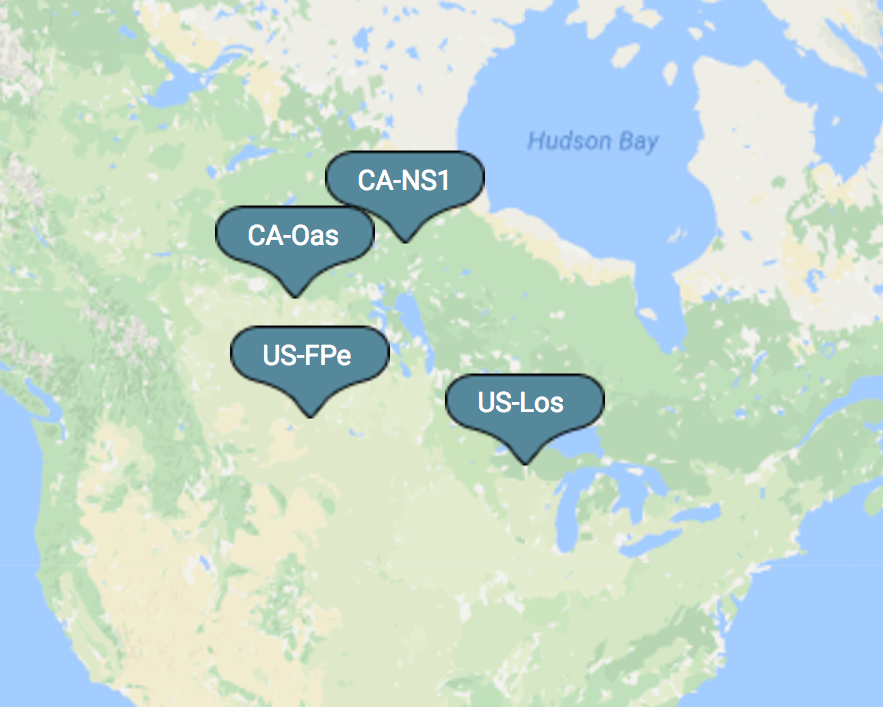
\includegraphics[width=\textwidth]{sites.png}
\end{figure}
\end{frame}


\begin{frame}
\frametitle{Sites}

\begin{center}
\begin{tabular}{| c | c | c | c | c |}
\hline
Name & Climate & Type & Mean T, C & Mean P, mm \\ \hline
CA-NS1 & Dfc & ENF & -2.89 & 500.29 \\\hline
CA-NS6 & Dfc & OSH & -3.08 & 495.37 \\\hline
CA-Oas & Dfc & DBF & 0.34 & 428.53 \\\hline
US-FPe & Bsk & GRA & 5.48 & 334.8 \\\hline
US-Los &  Dfb& WET &   4.08 & 828\\\hline

\hline
\end{tabular}
\end{center}


\textbf{Climate}:
Dfc - Subarctic: severe winter, no dry season, cool summer;
Bsk - Cold semi-arid climate, steppe, warm winter;
Dfb - Warm Summer Continental: significant precipitation in all seasons.

\textbf{Vegetation}:
ENF - Evergreen Needleleaf Forests;
OSH - Open Shrublands;
DBF - Deciduous Broadleaf Forests;
GRA - grassland;
WET - Permanent Wetlands.


\end{frame}


\begin{frame}
\frametitle{Flux in Time}

\begin{columns}[t]
\column{.35\textwidth}
\centering
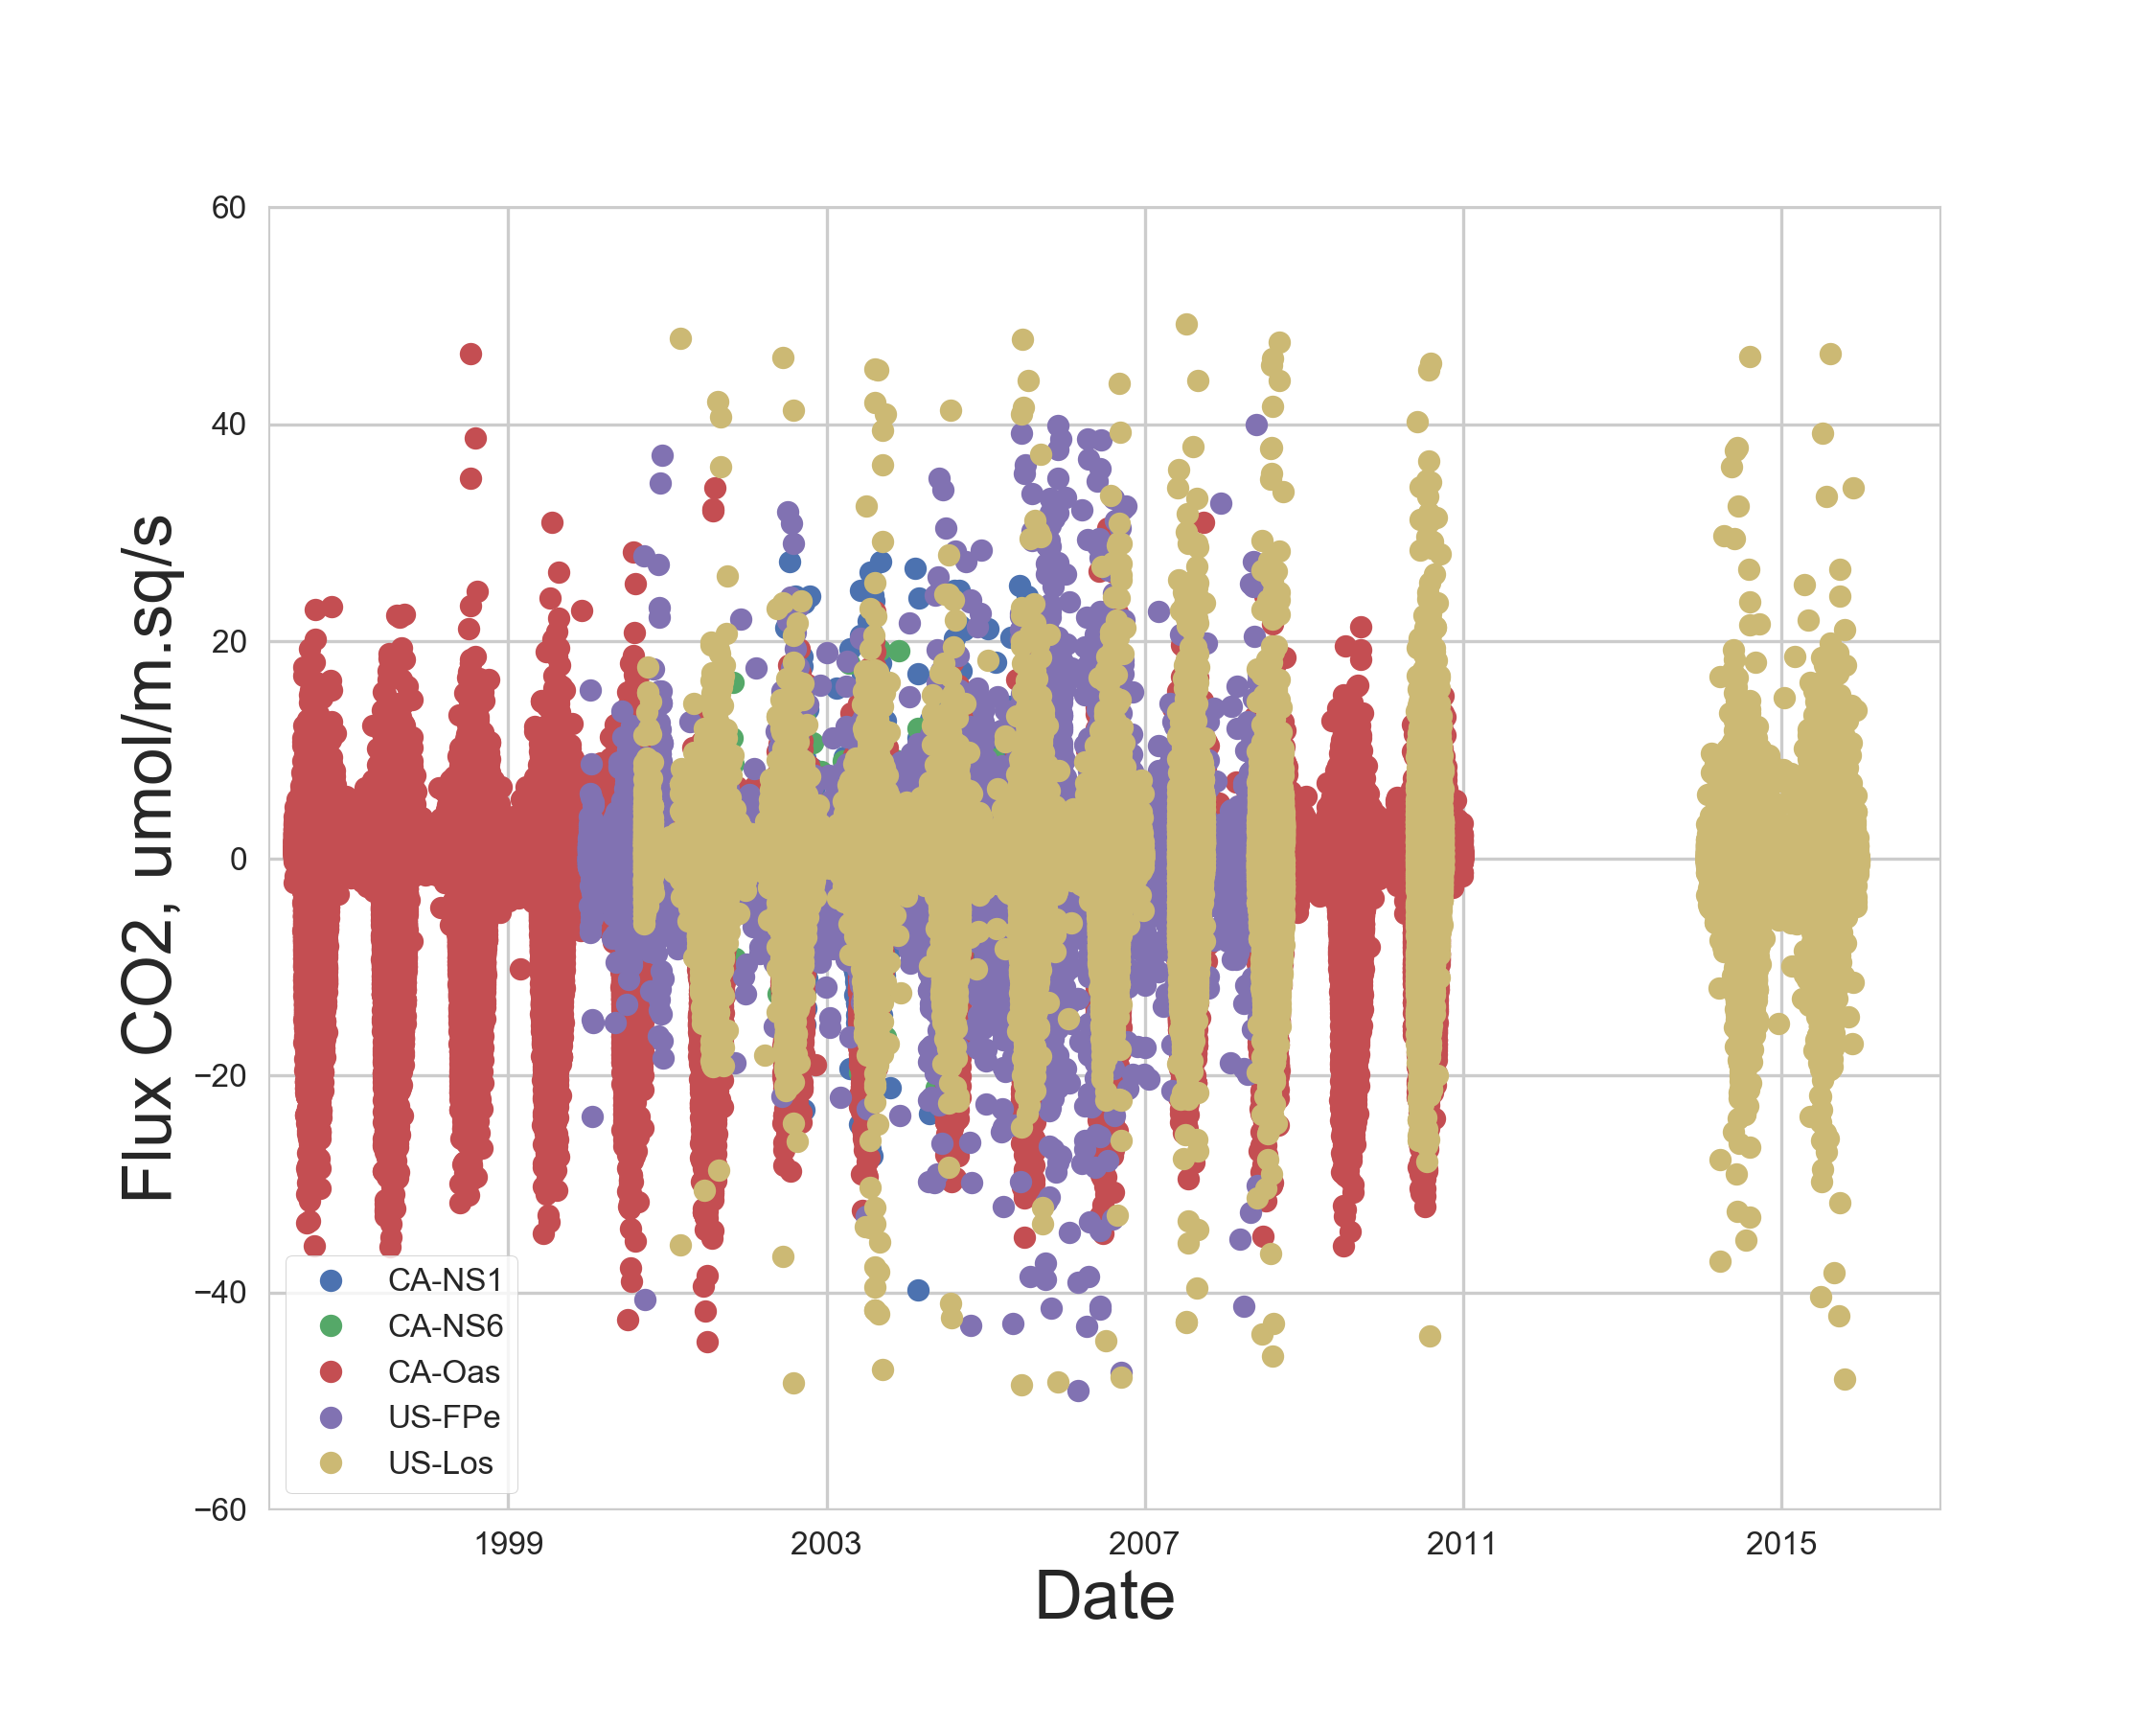
\includegraphics[width=\textwidth]{FvsTime/all.png}\\
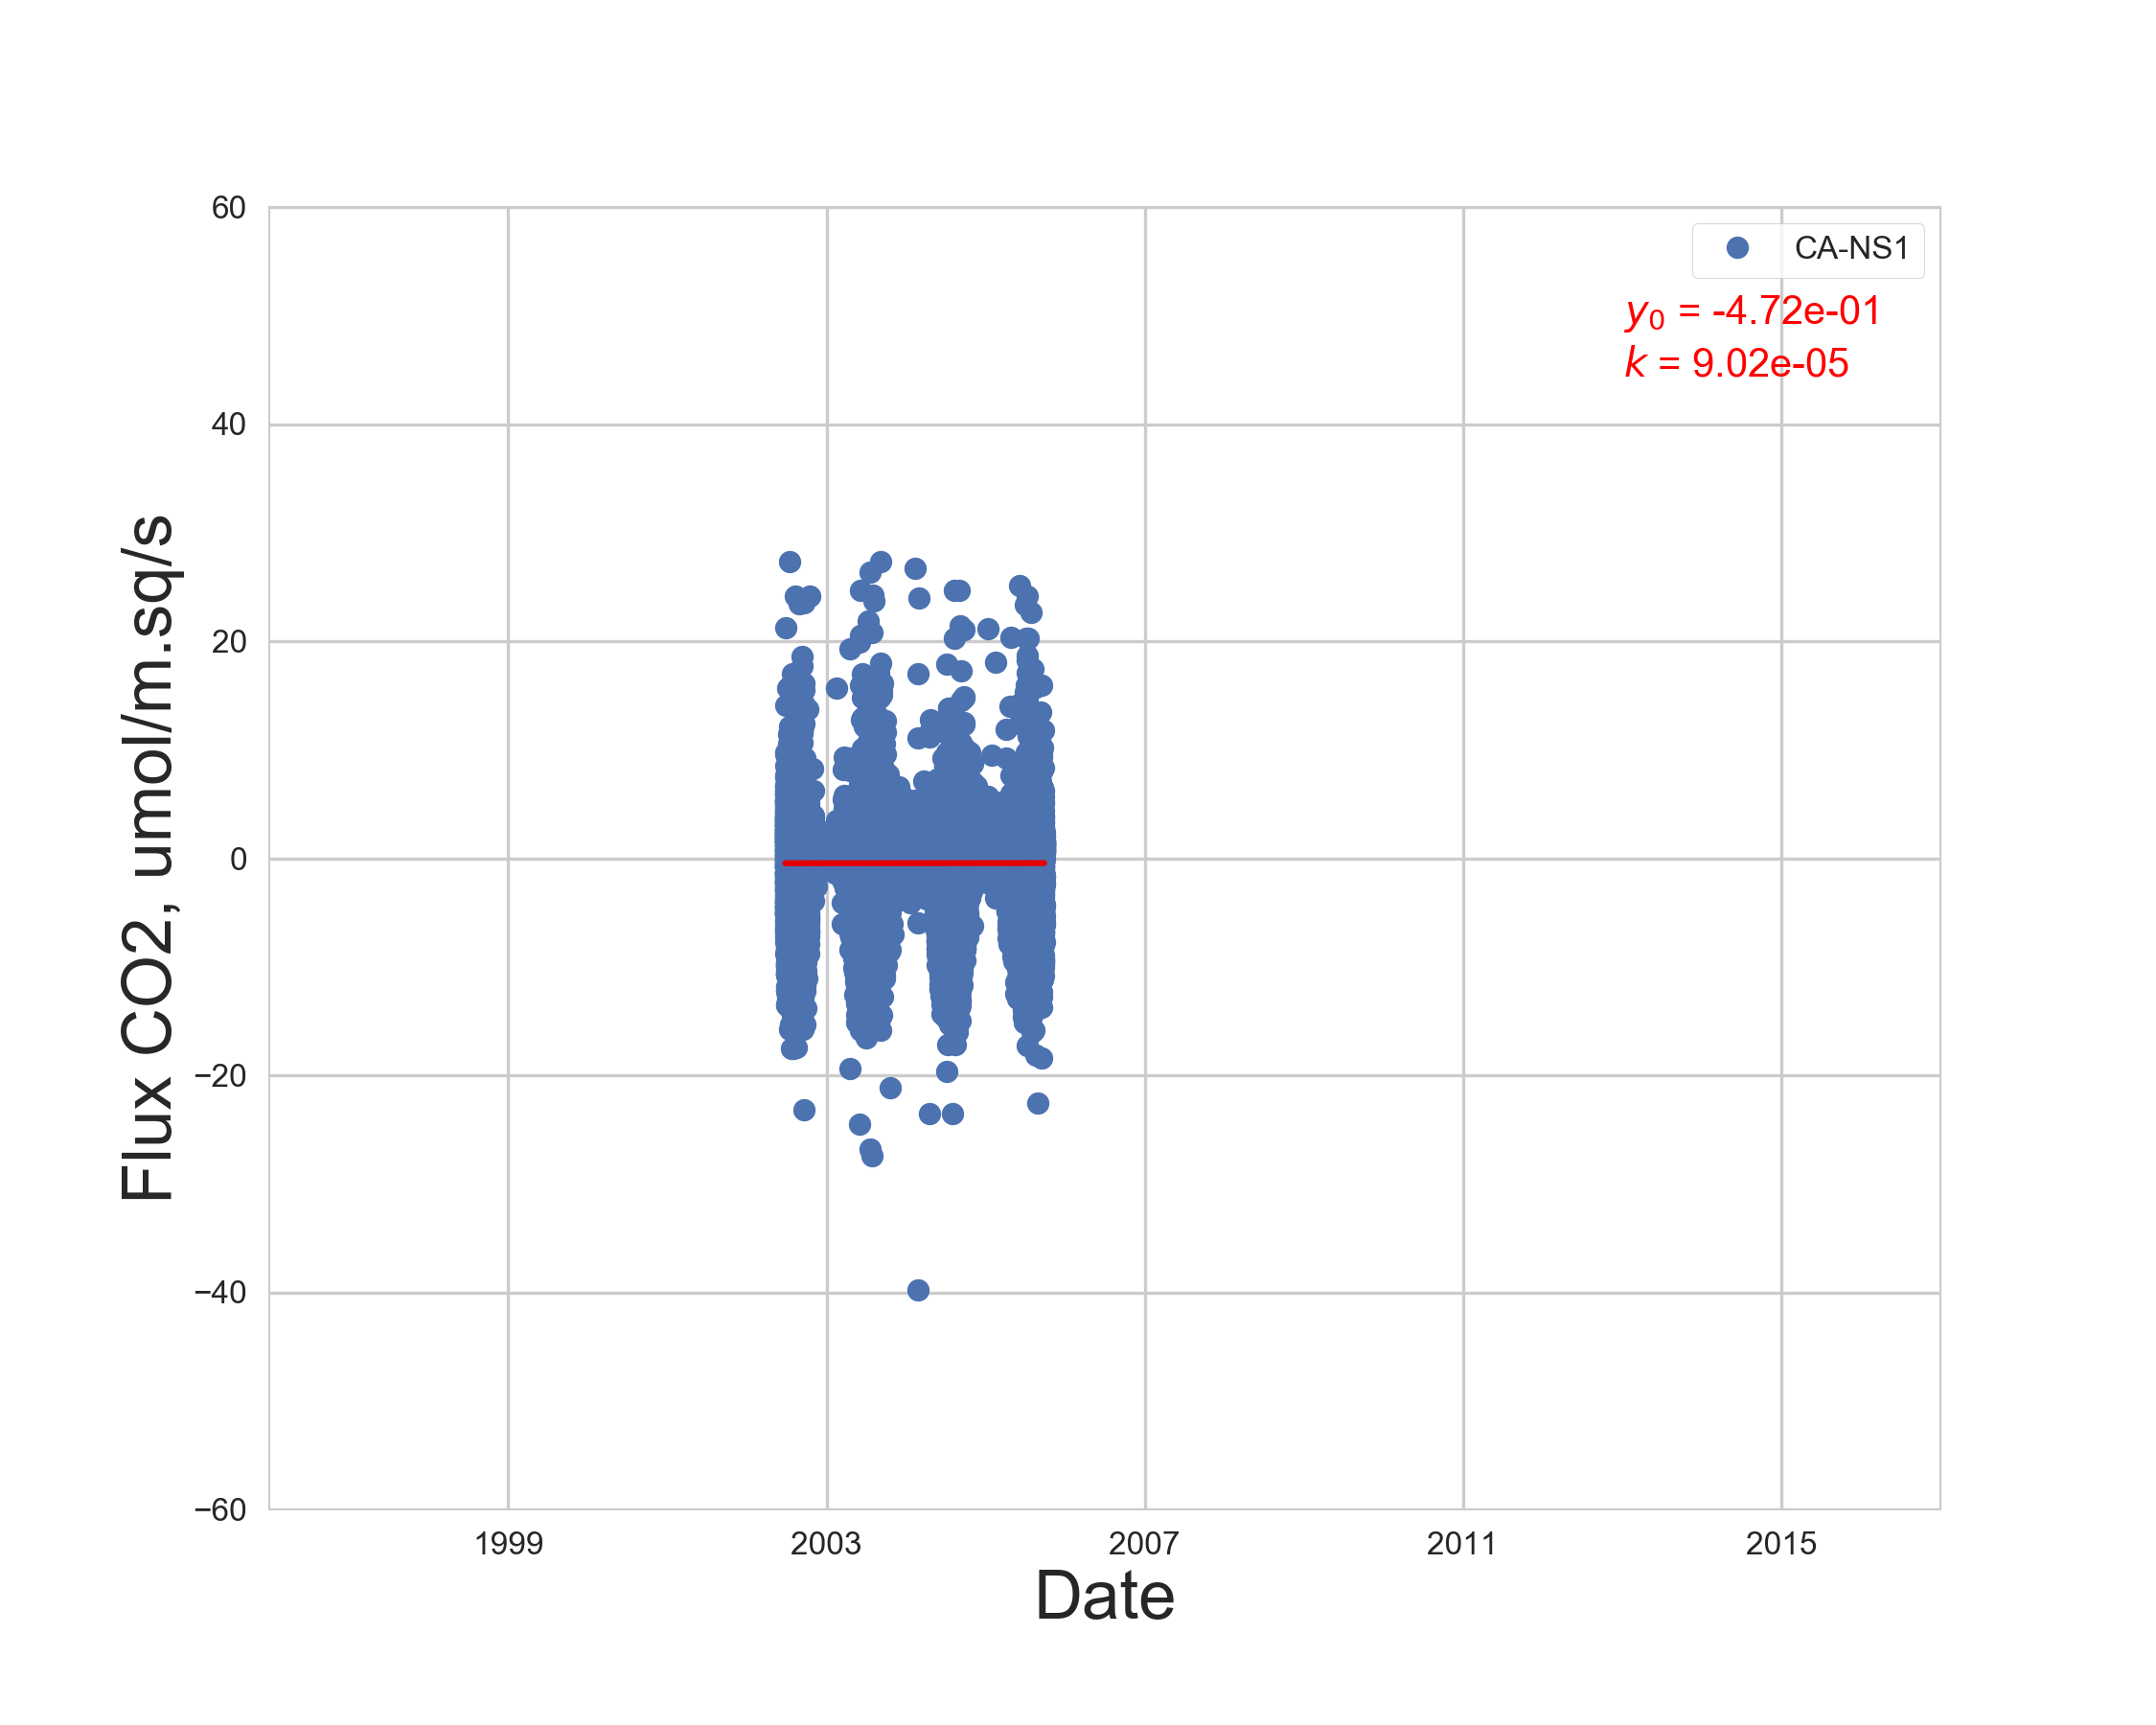
\includegraphics[width=\textwidth]{FvsTime/CA-NS1.png}
\column{.35\textwidth}
\centering
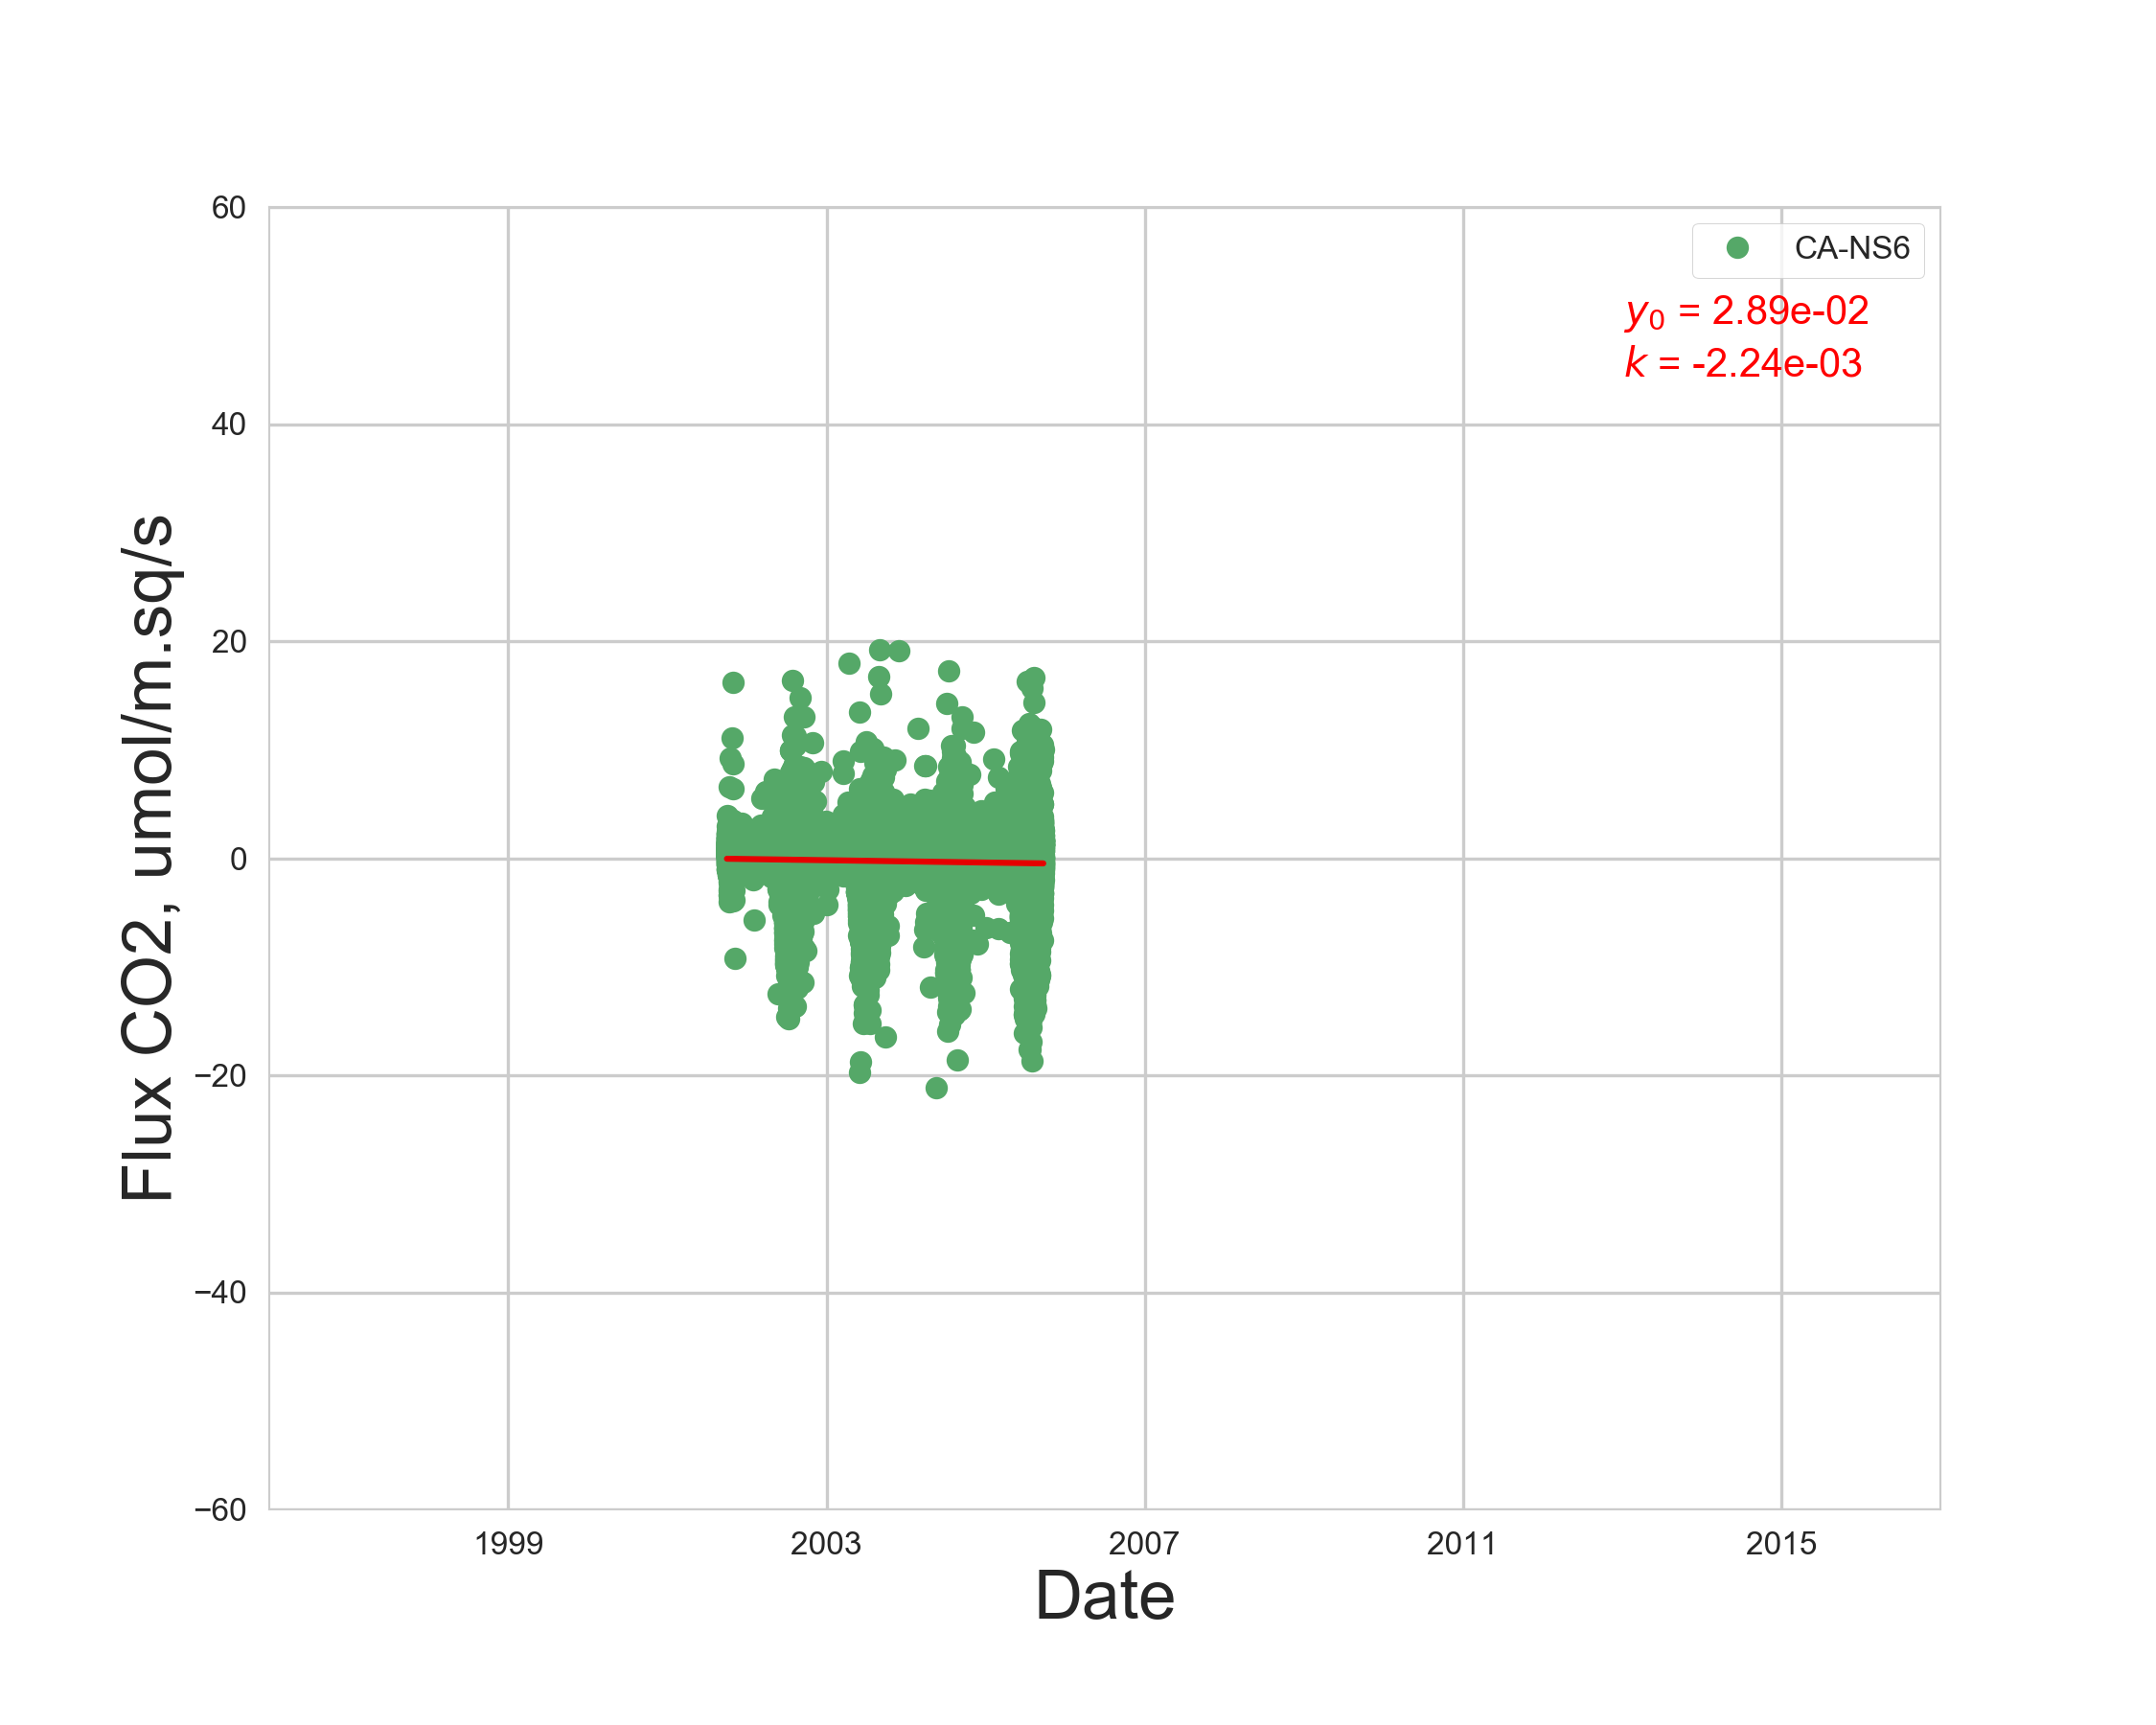
\includegraphics[width=\textwidth]{FvsTime/CA-NS6.png}\\
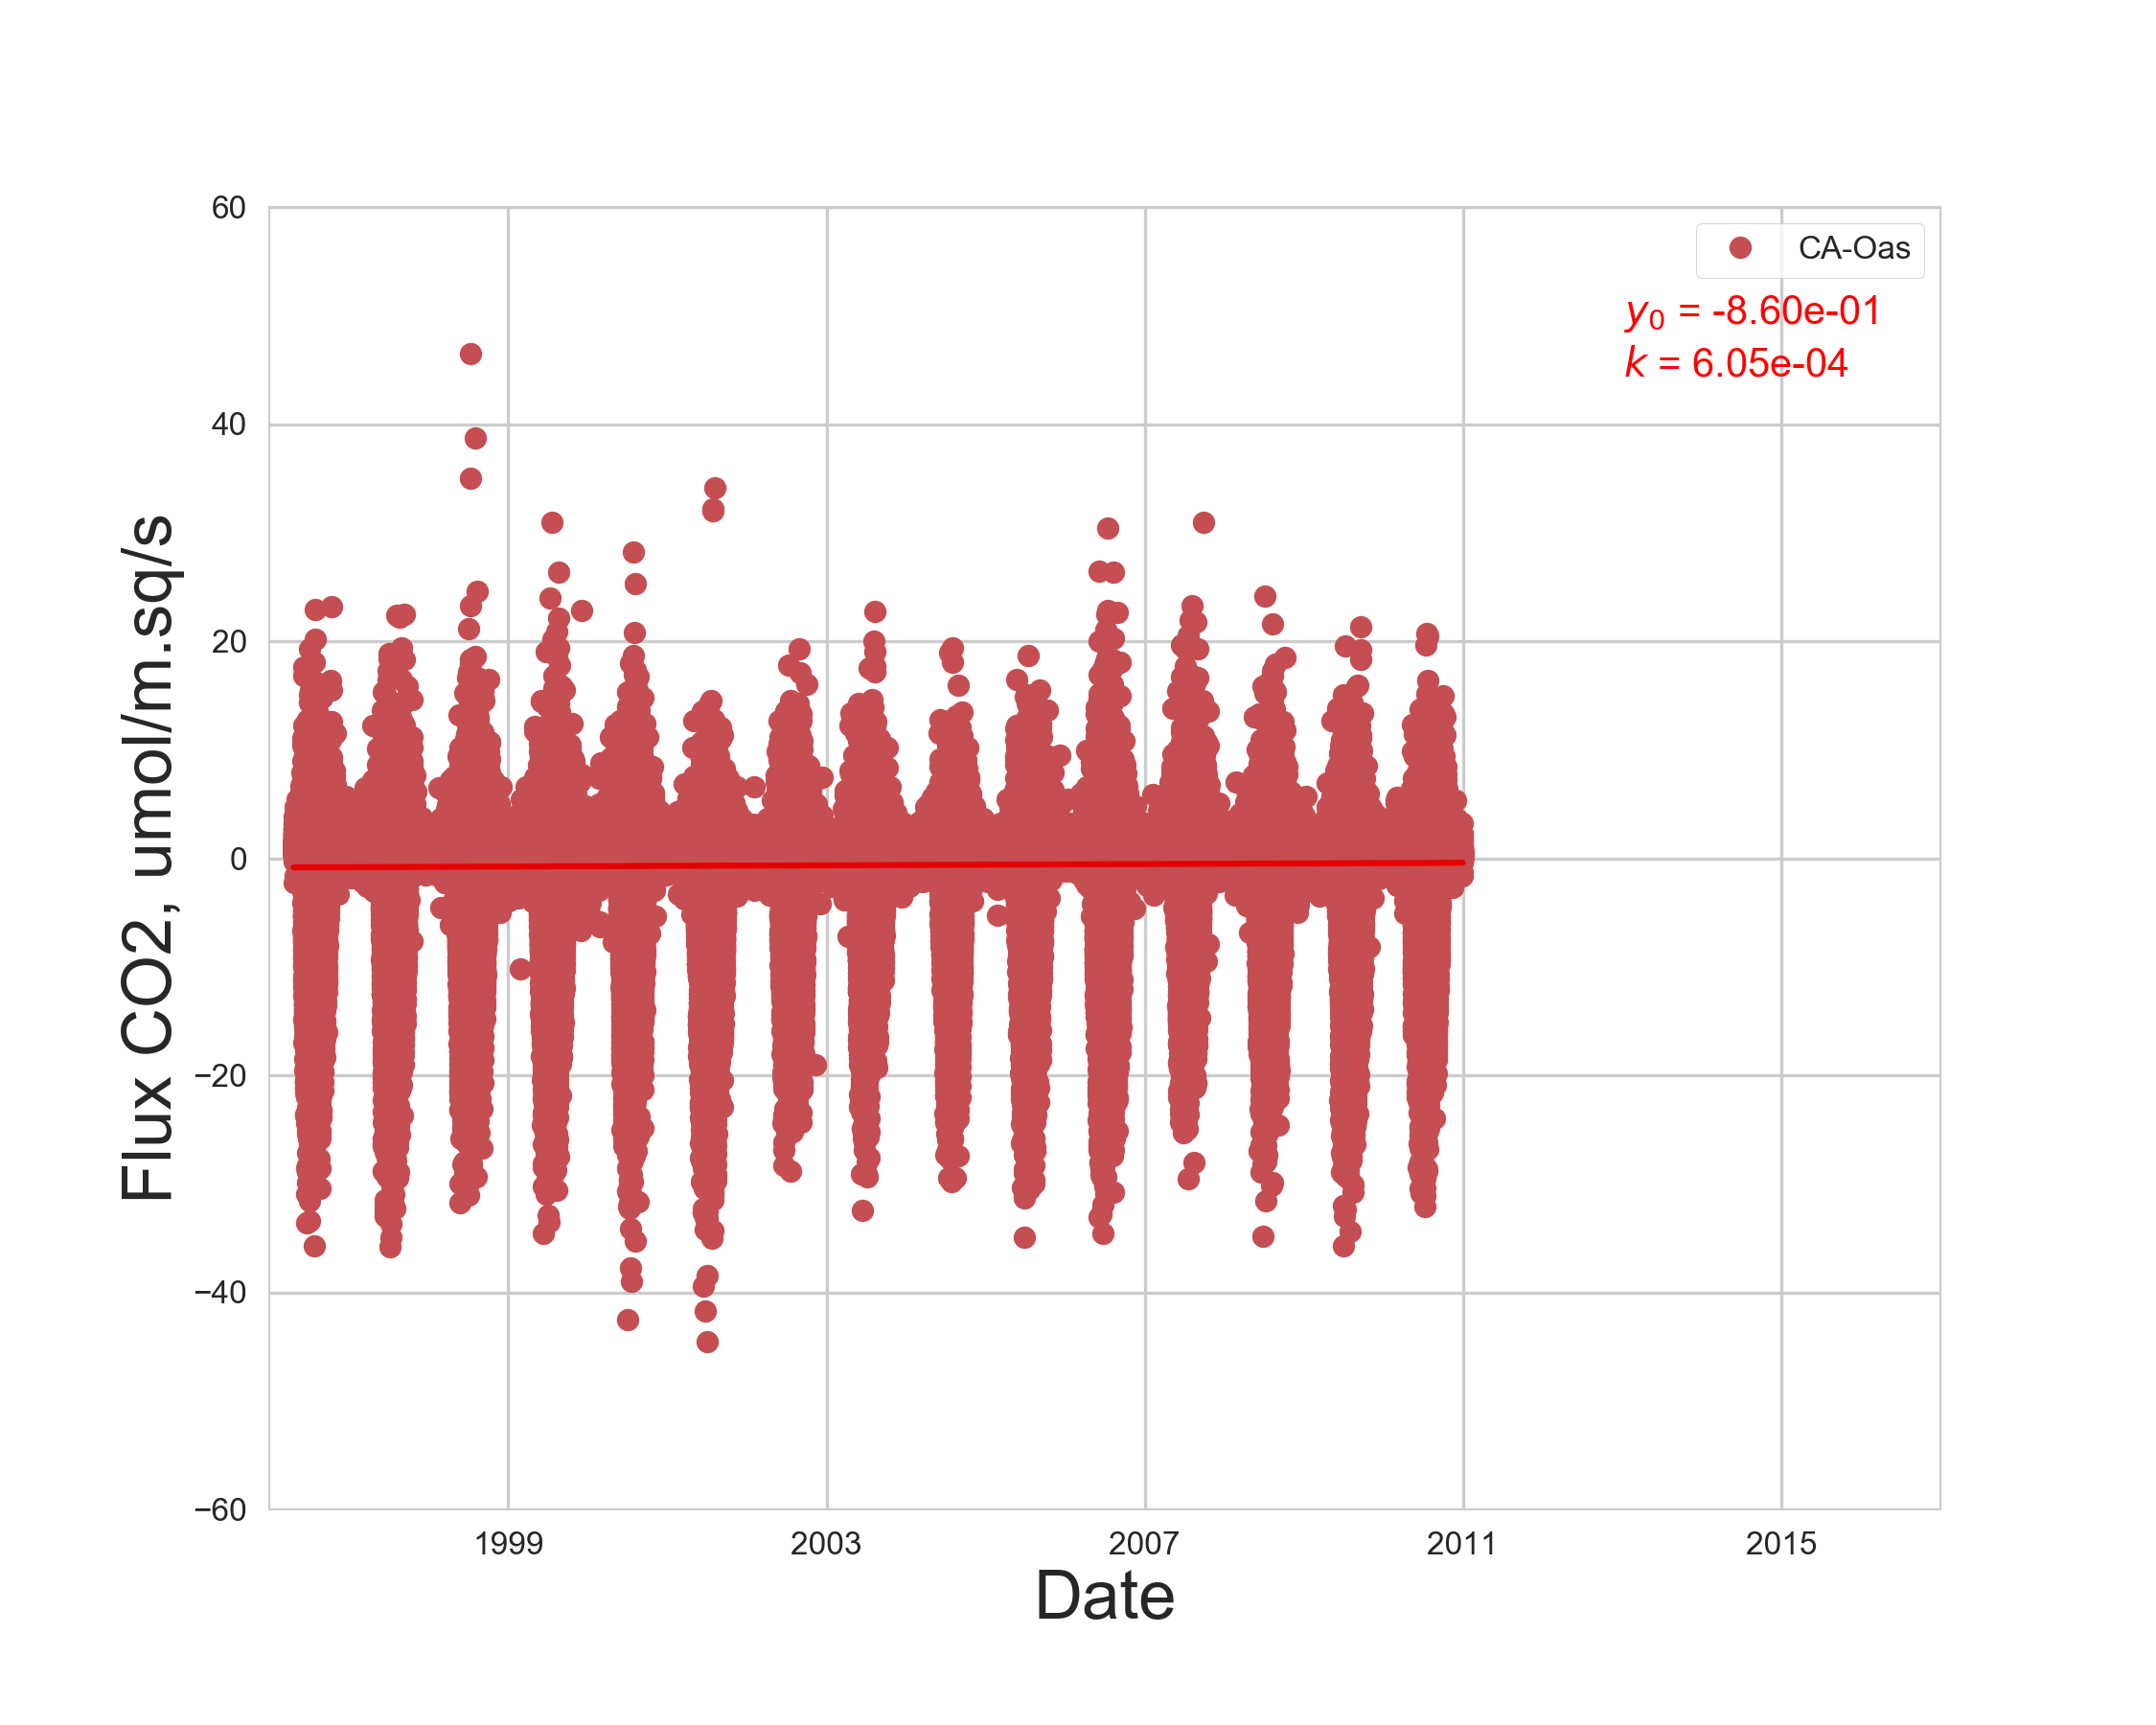
\includegraphics[width=\textwidth]{FvsTime/CA-Oas.png}
\column{.35\textwidth}
\centering
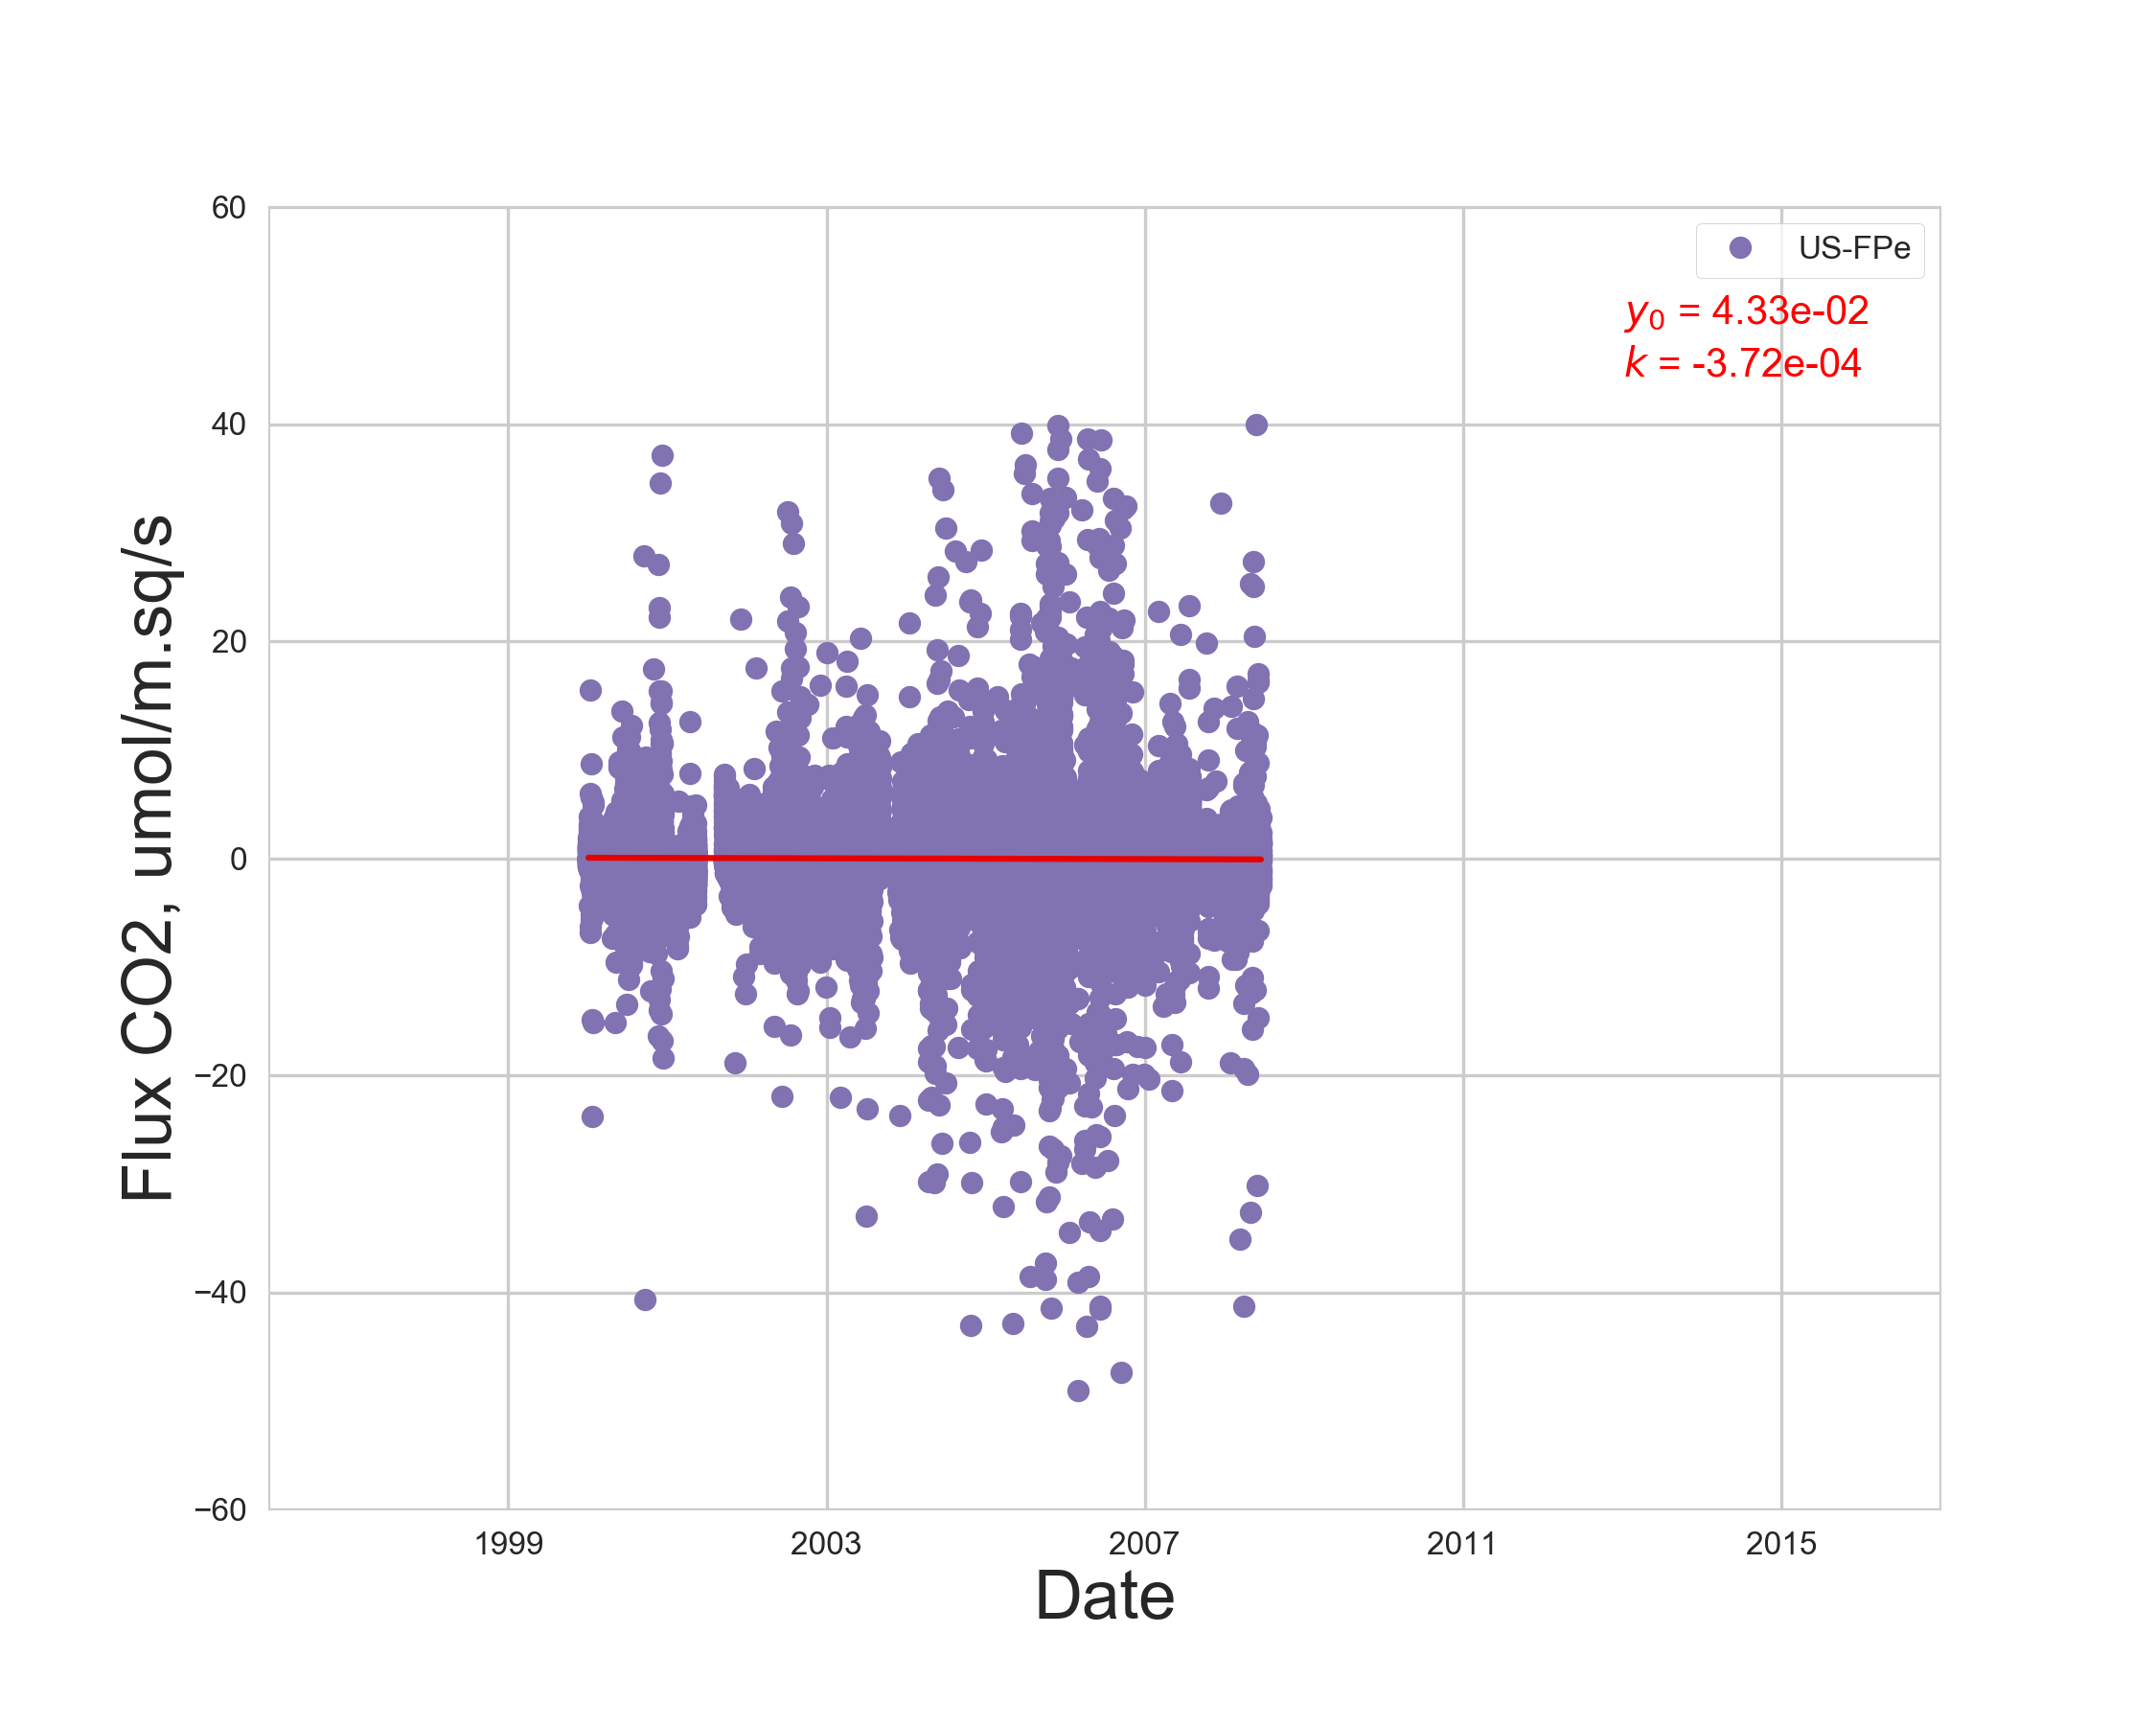
\includegraphics[width=\textwidth]{FvsTime/US-FPe.png}\\
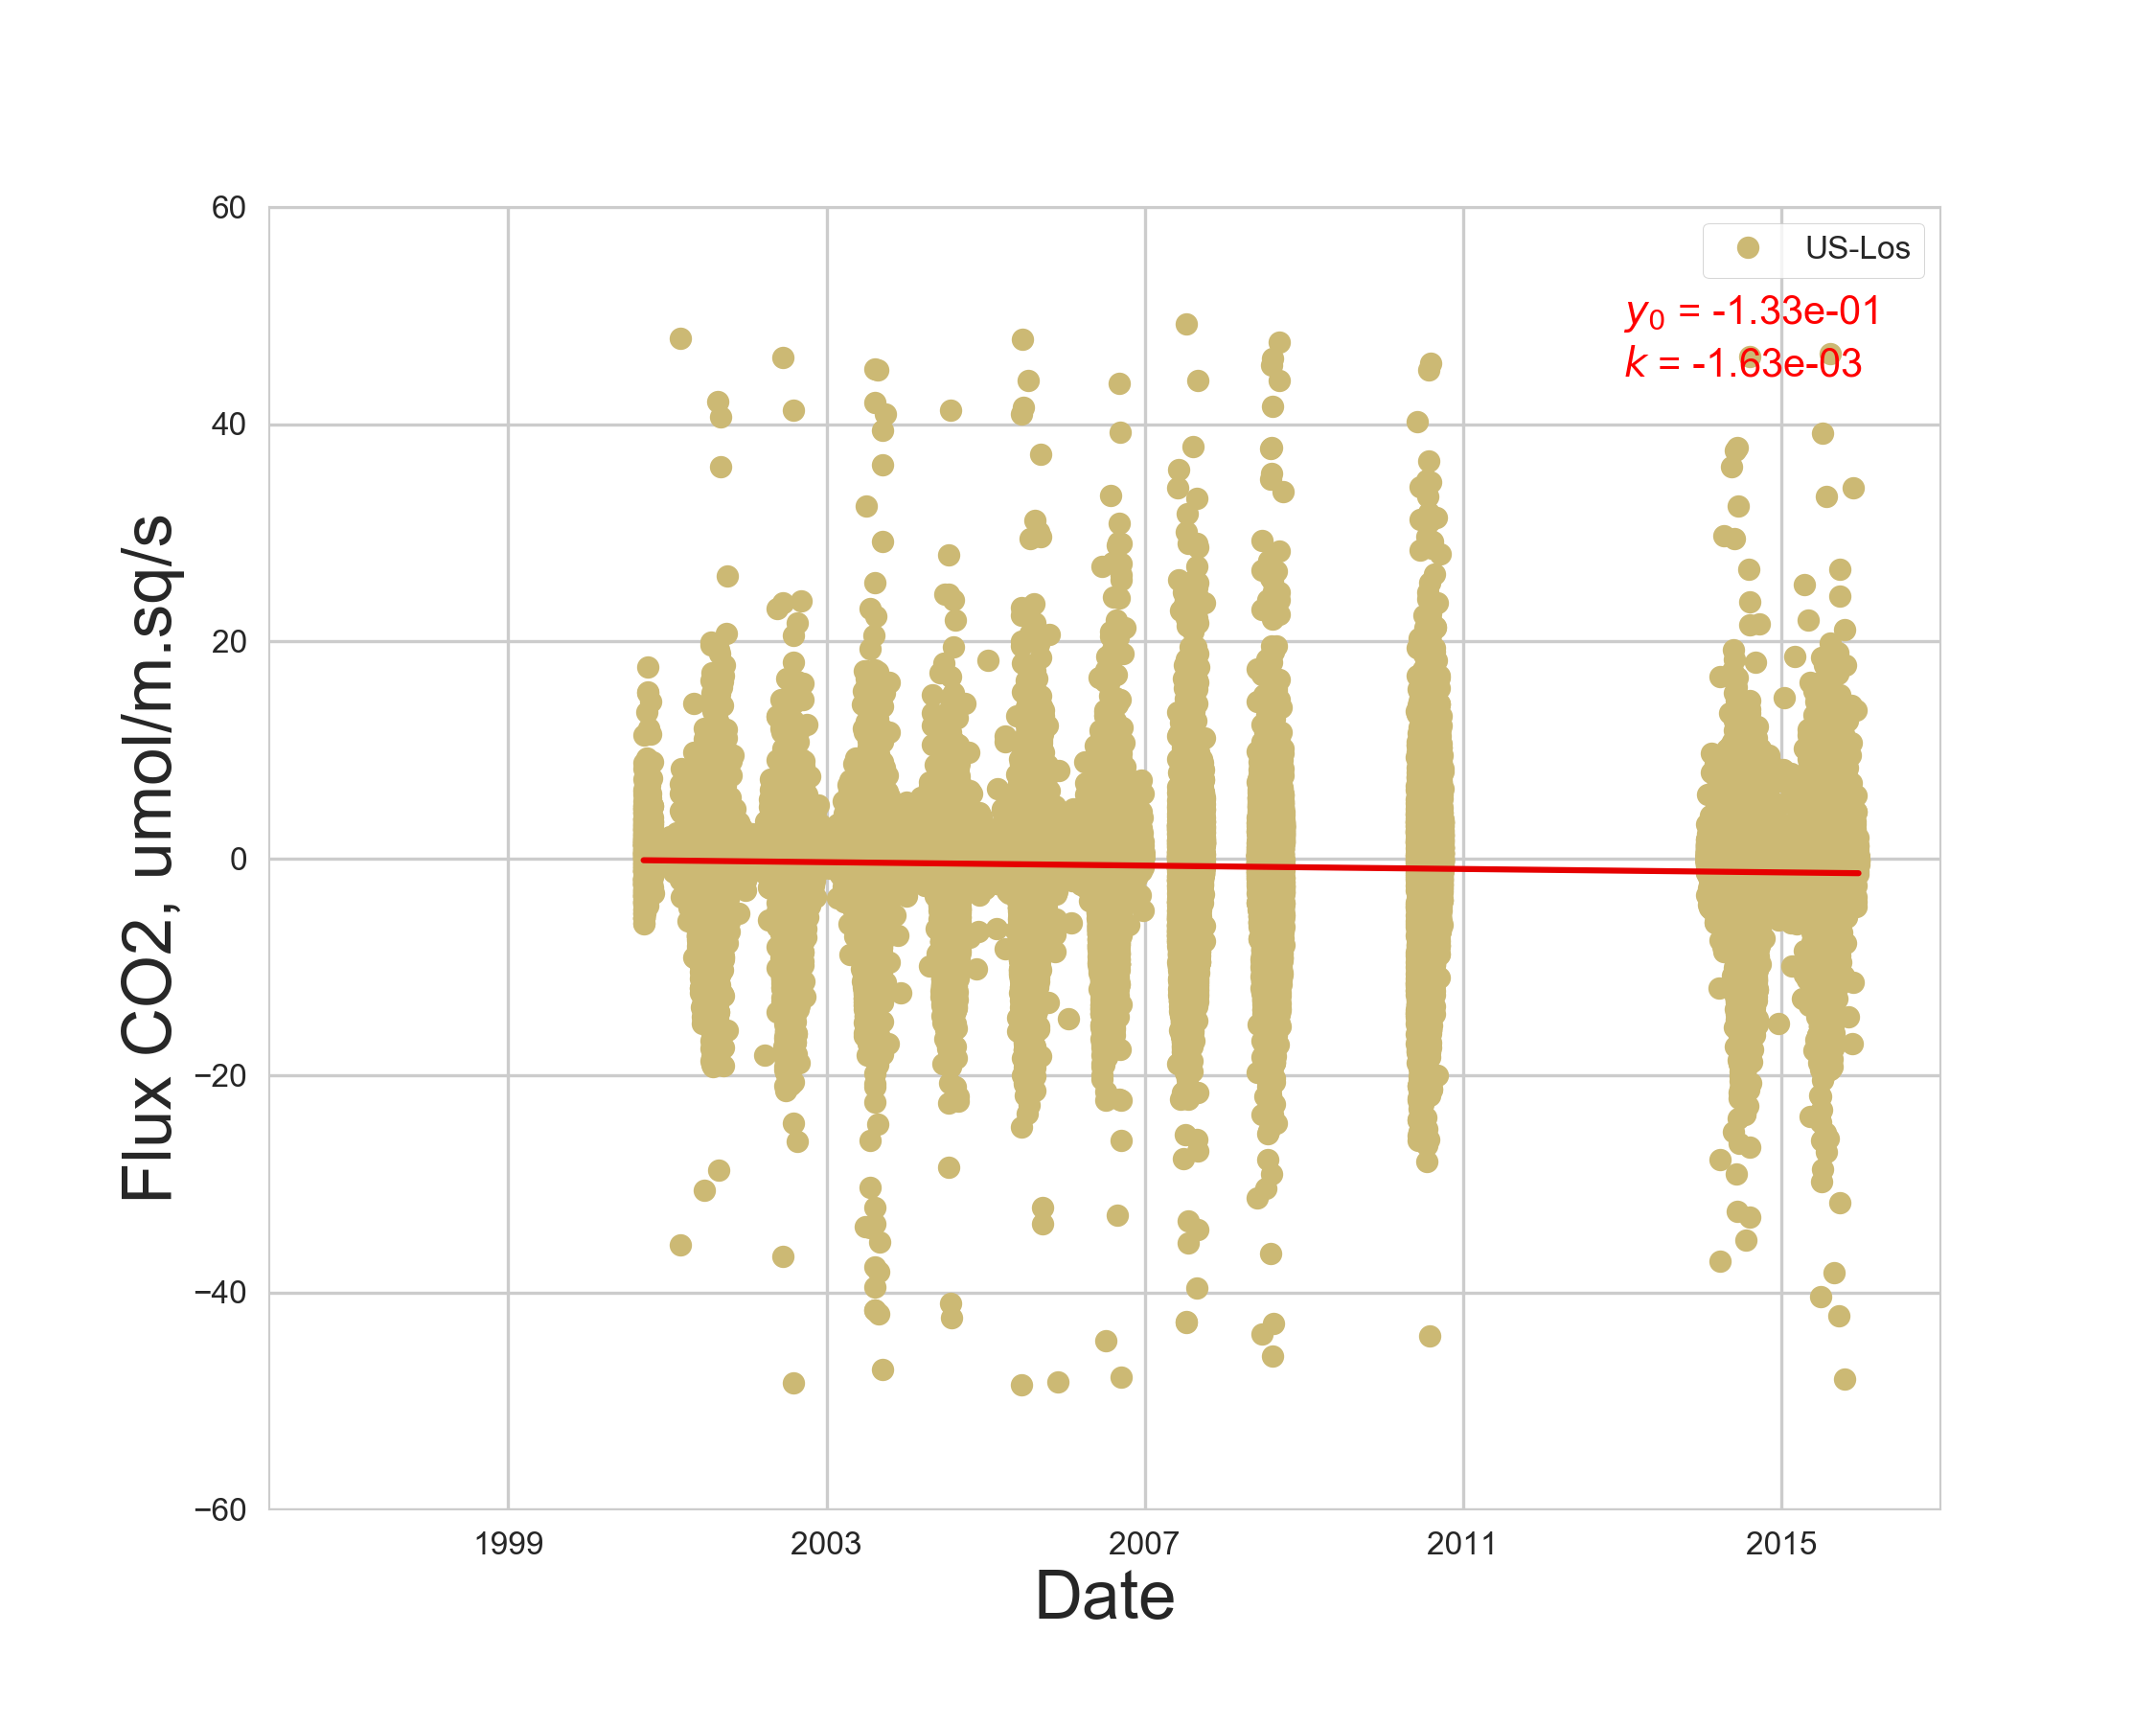
\includegraphics[width=\textwidth]{FvsTime/US-Los.png}
\end{columns}

\end{frame}


\begin{frame}
\frametitle{Density of Measurements}

\begin{columns}[t]
\column{.35\textwidth}
\centering
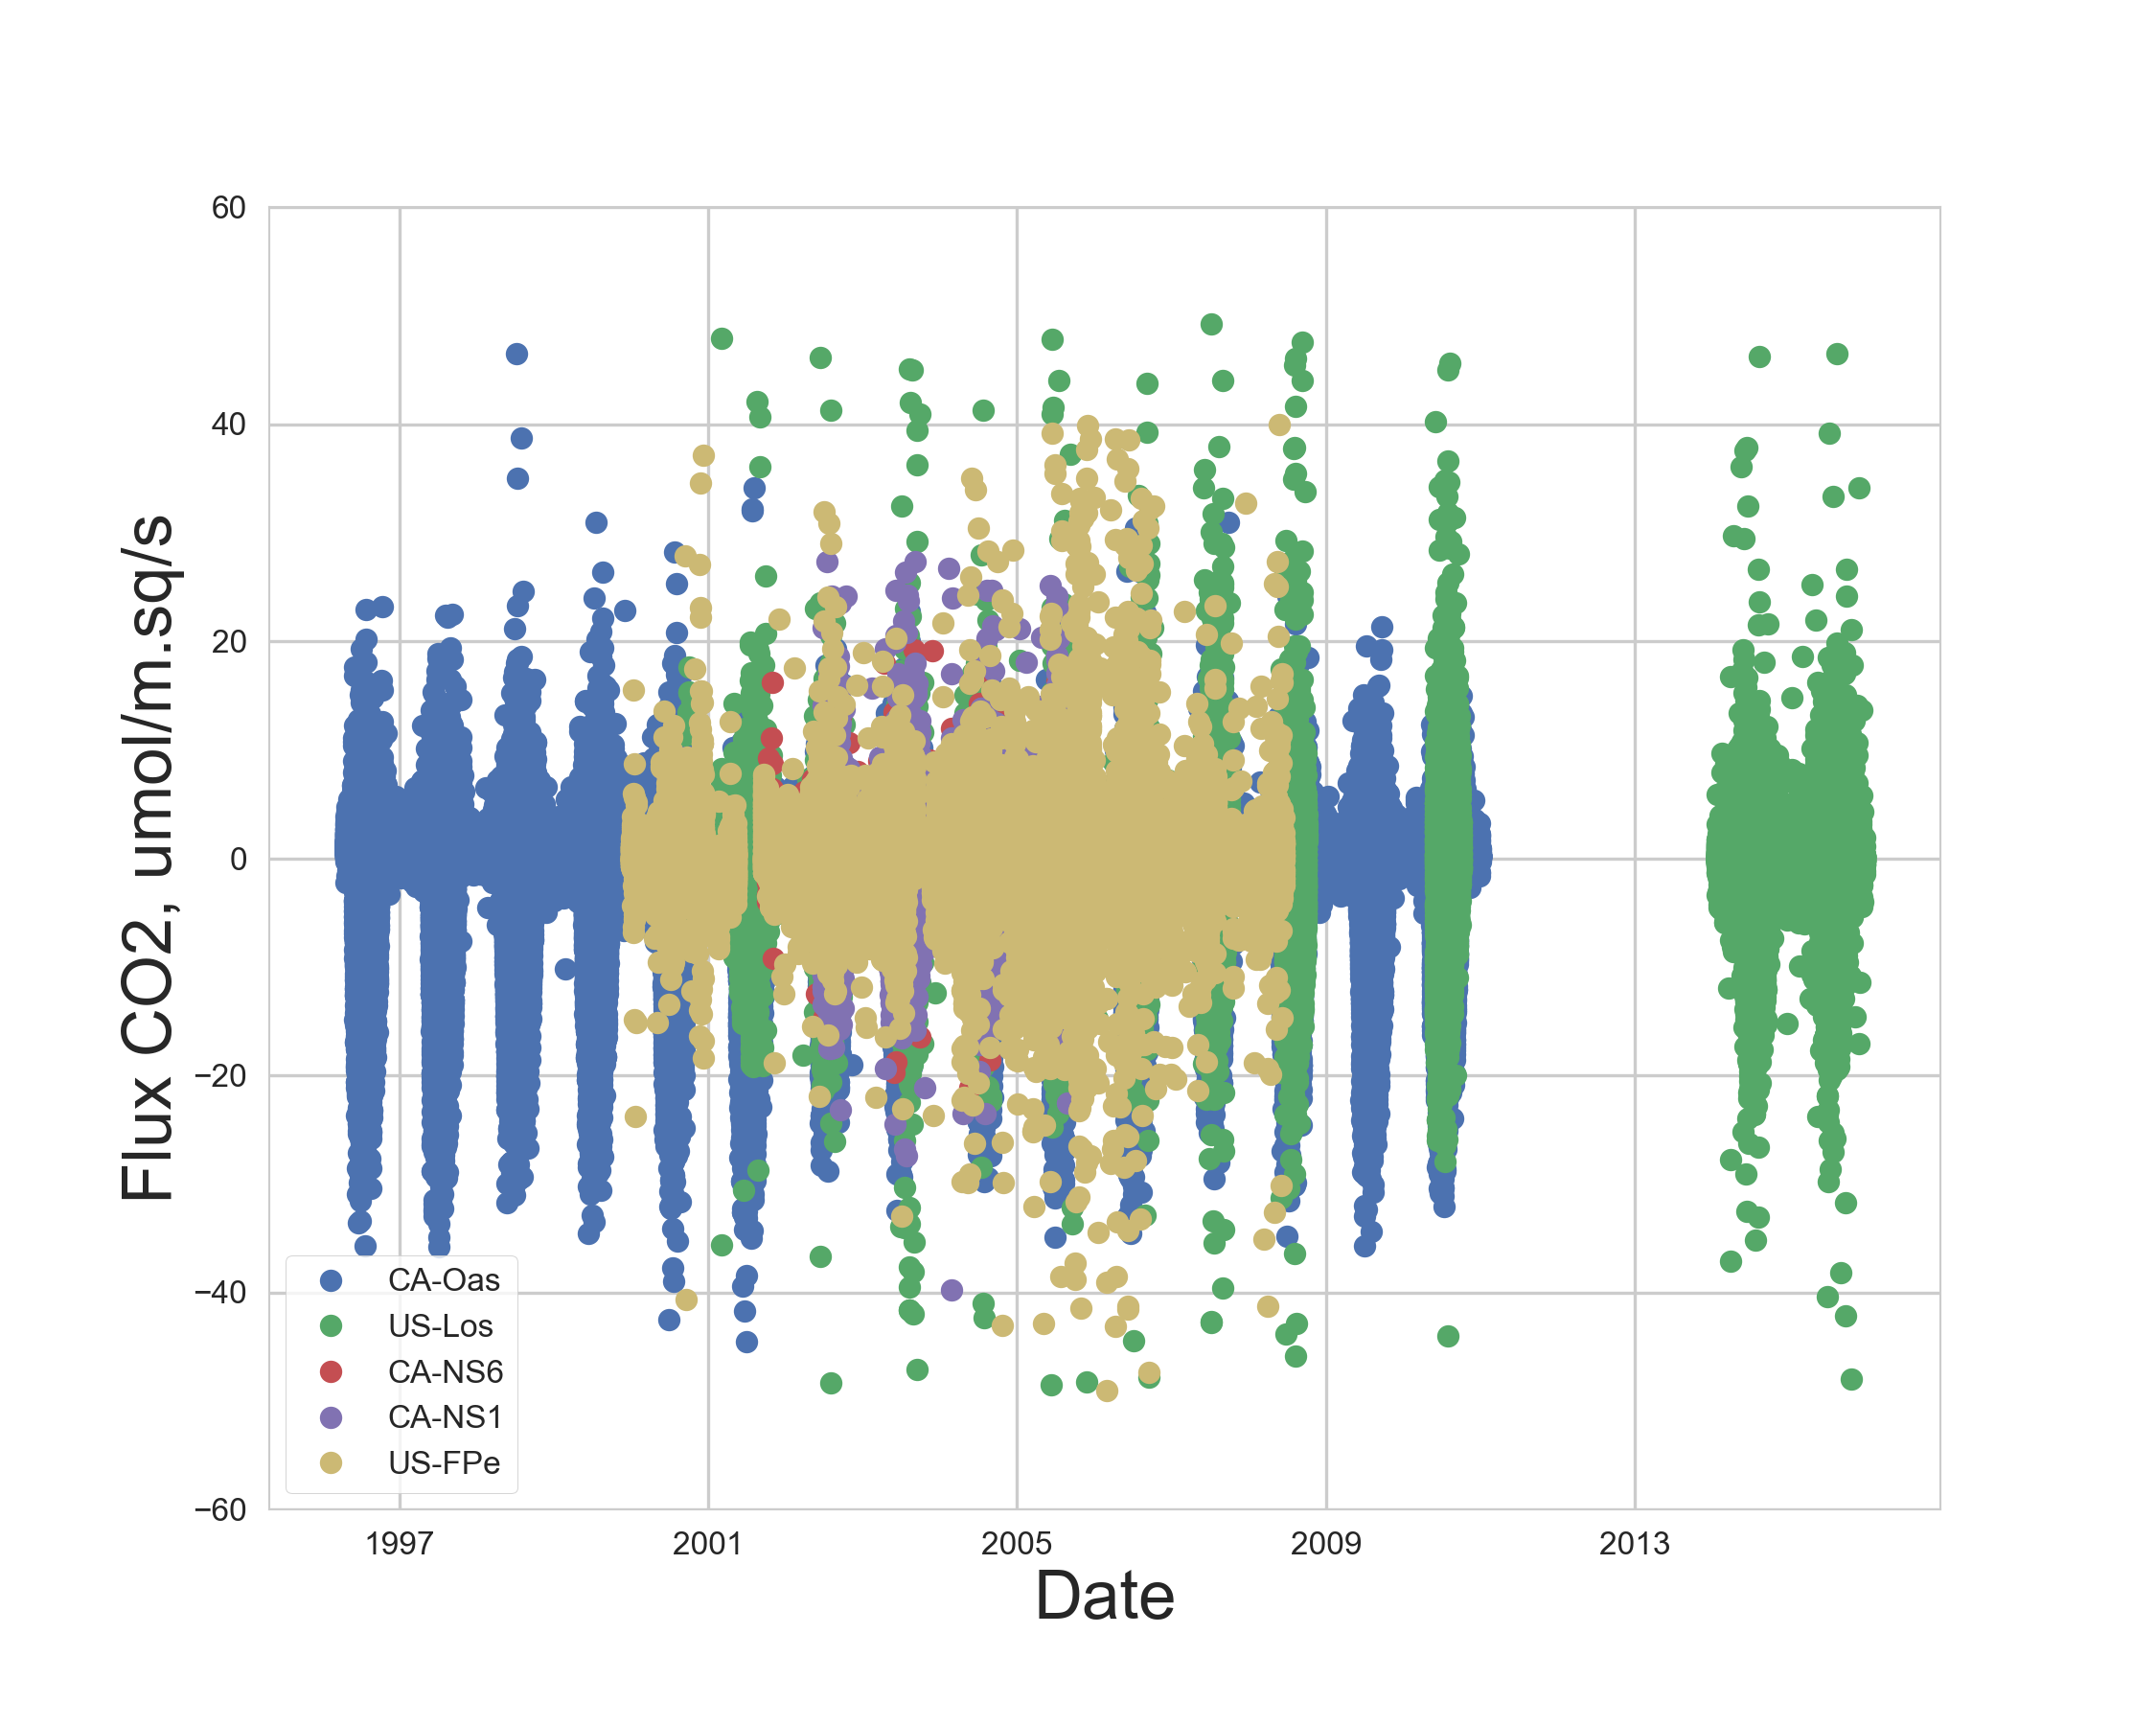
\includegraphics[width=\textwidth]{FvsTimeDen/all.png}\\
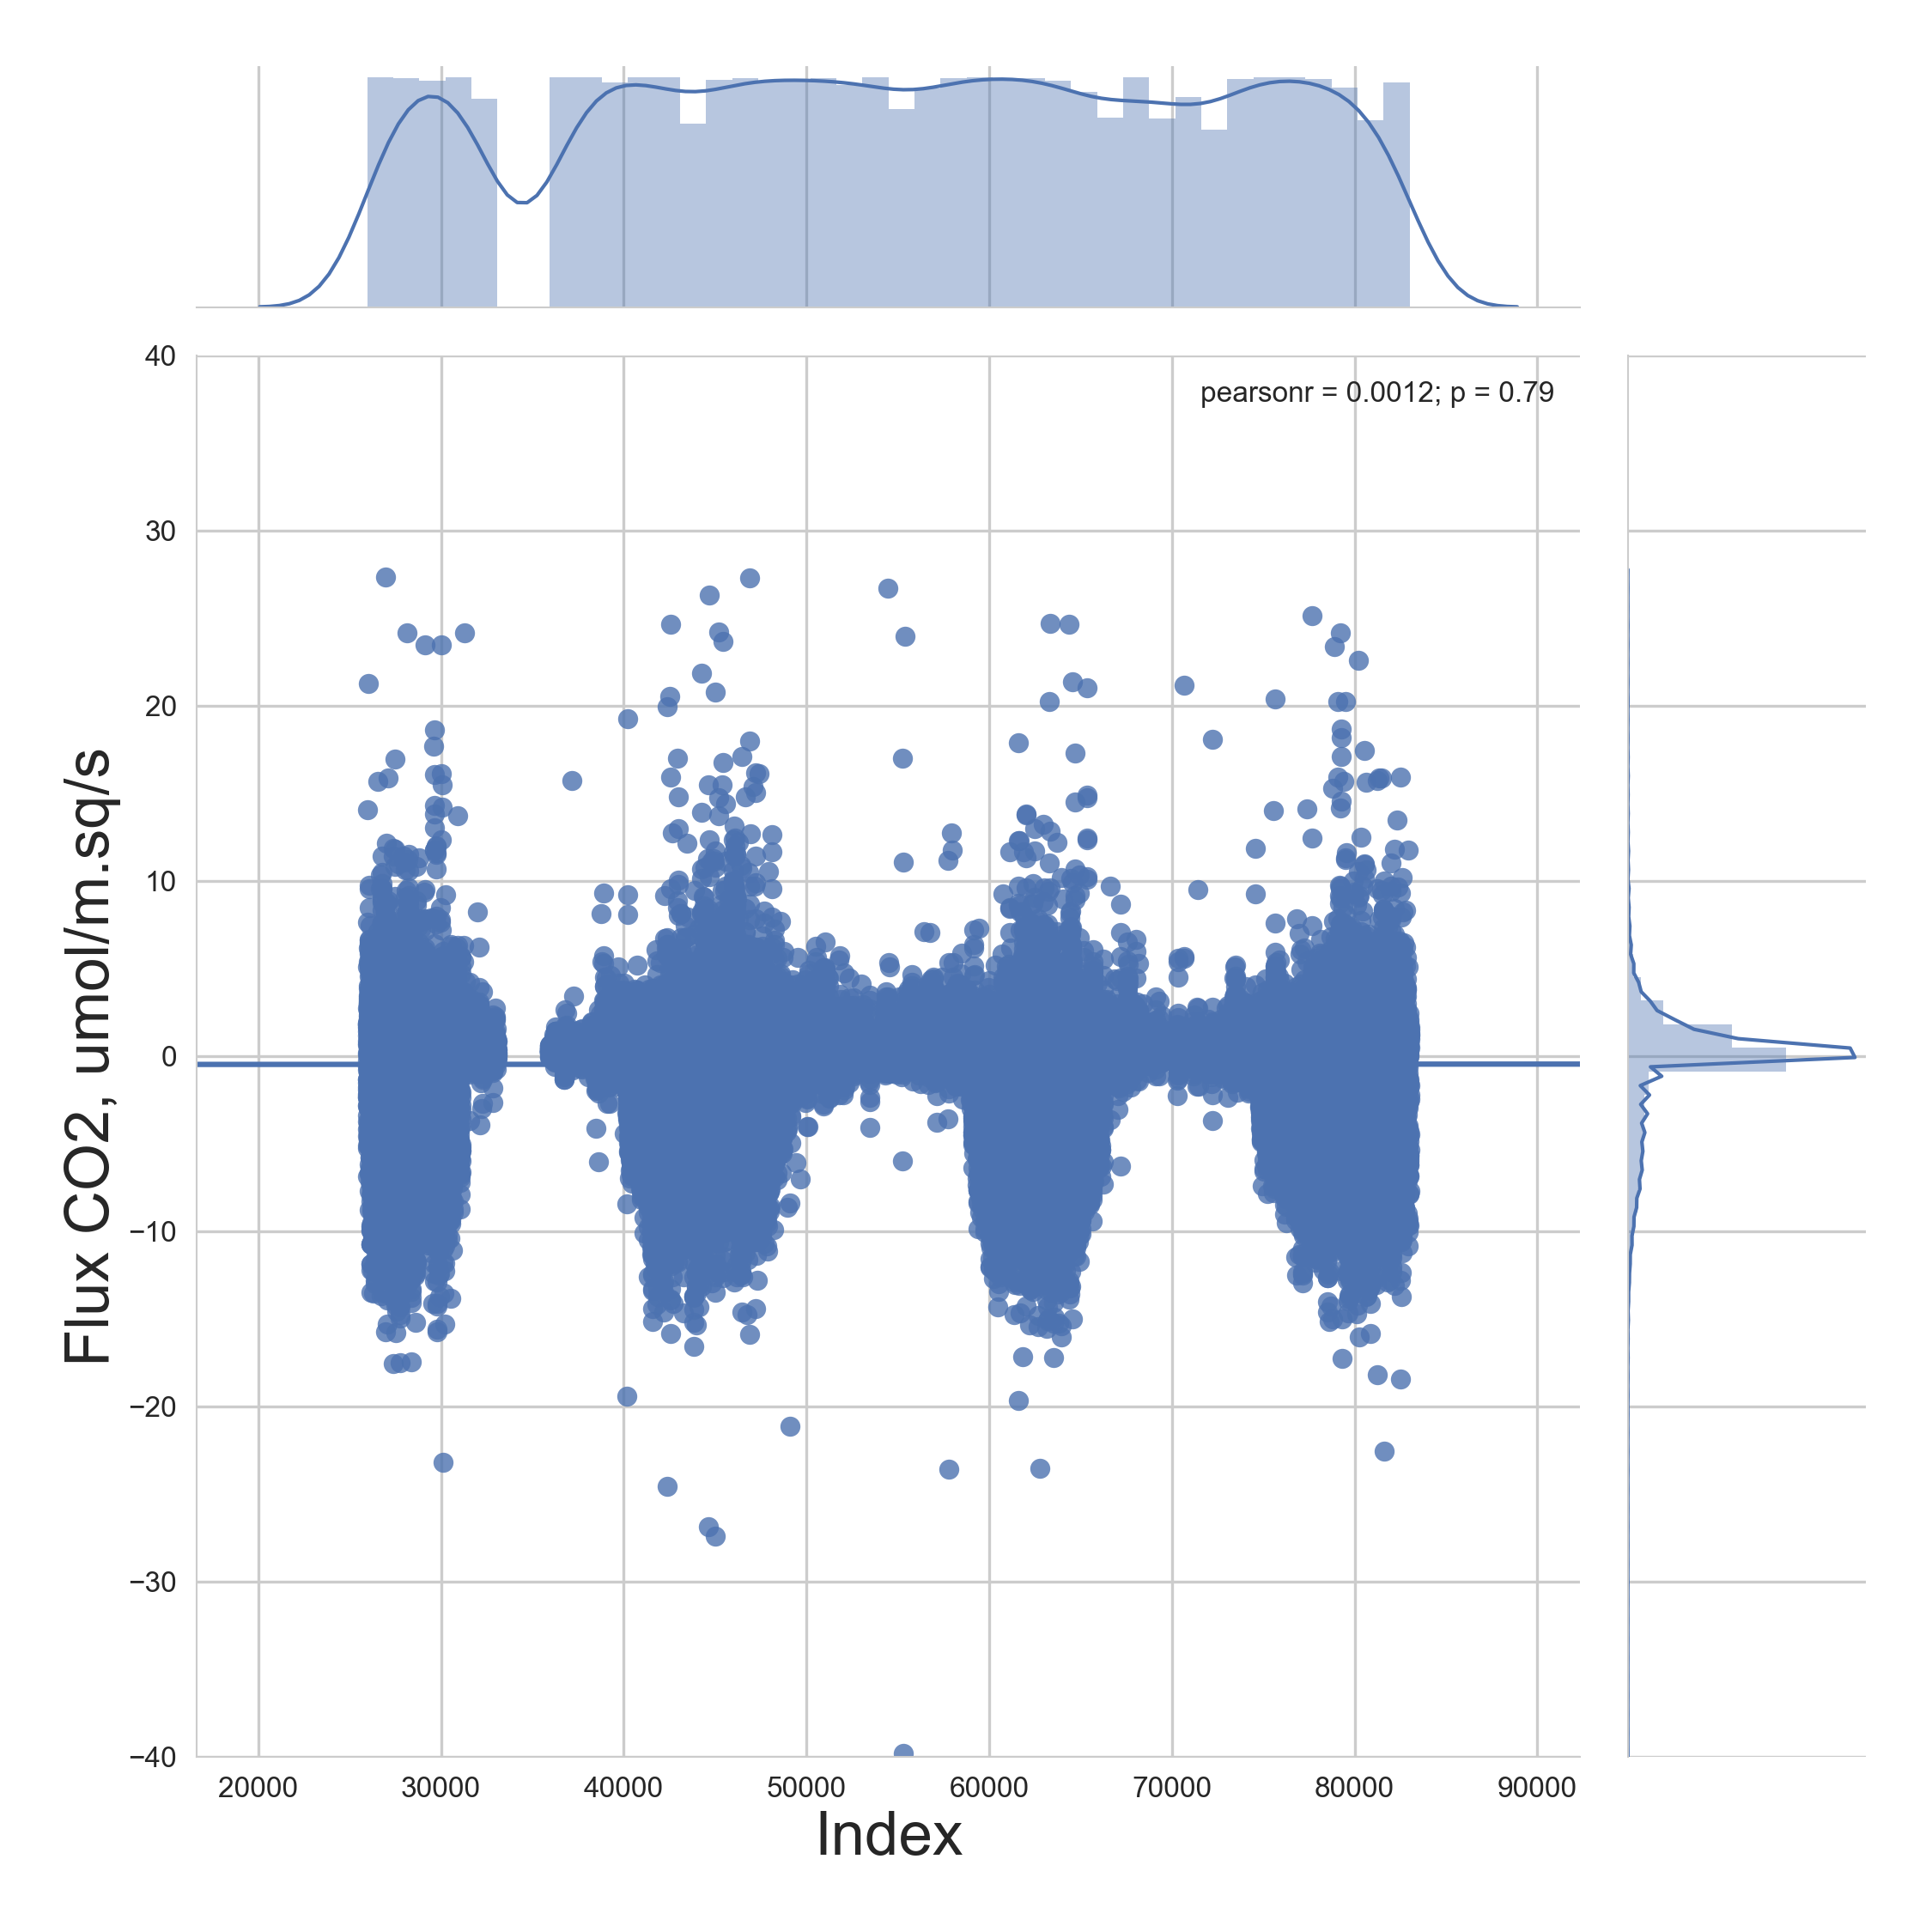
\includegraphics[width=\textwidth]{FvsTimeDen/CA-NS1.png}
\column{.35\textwidth}
\centering
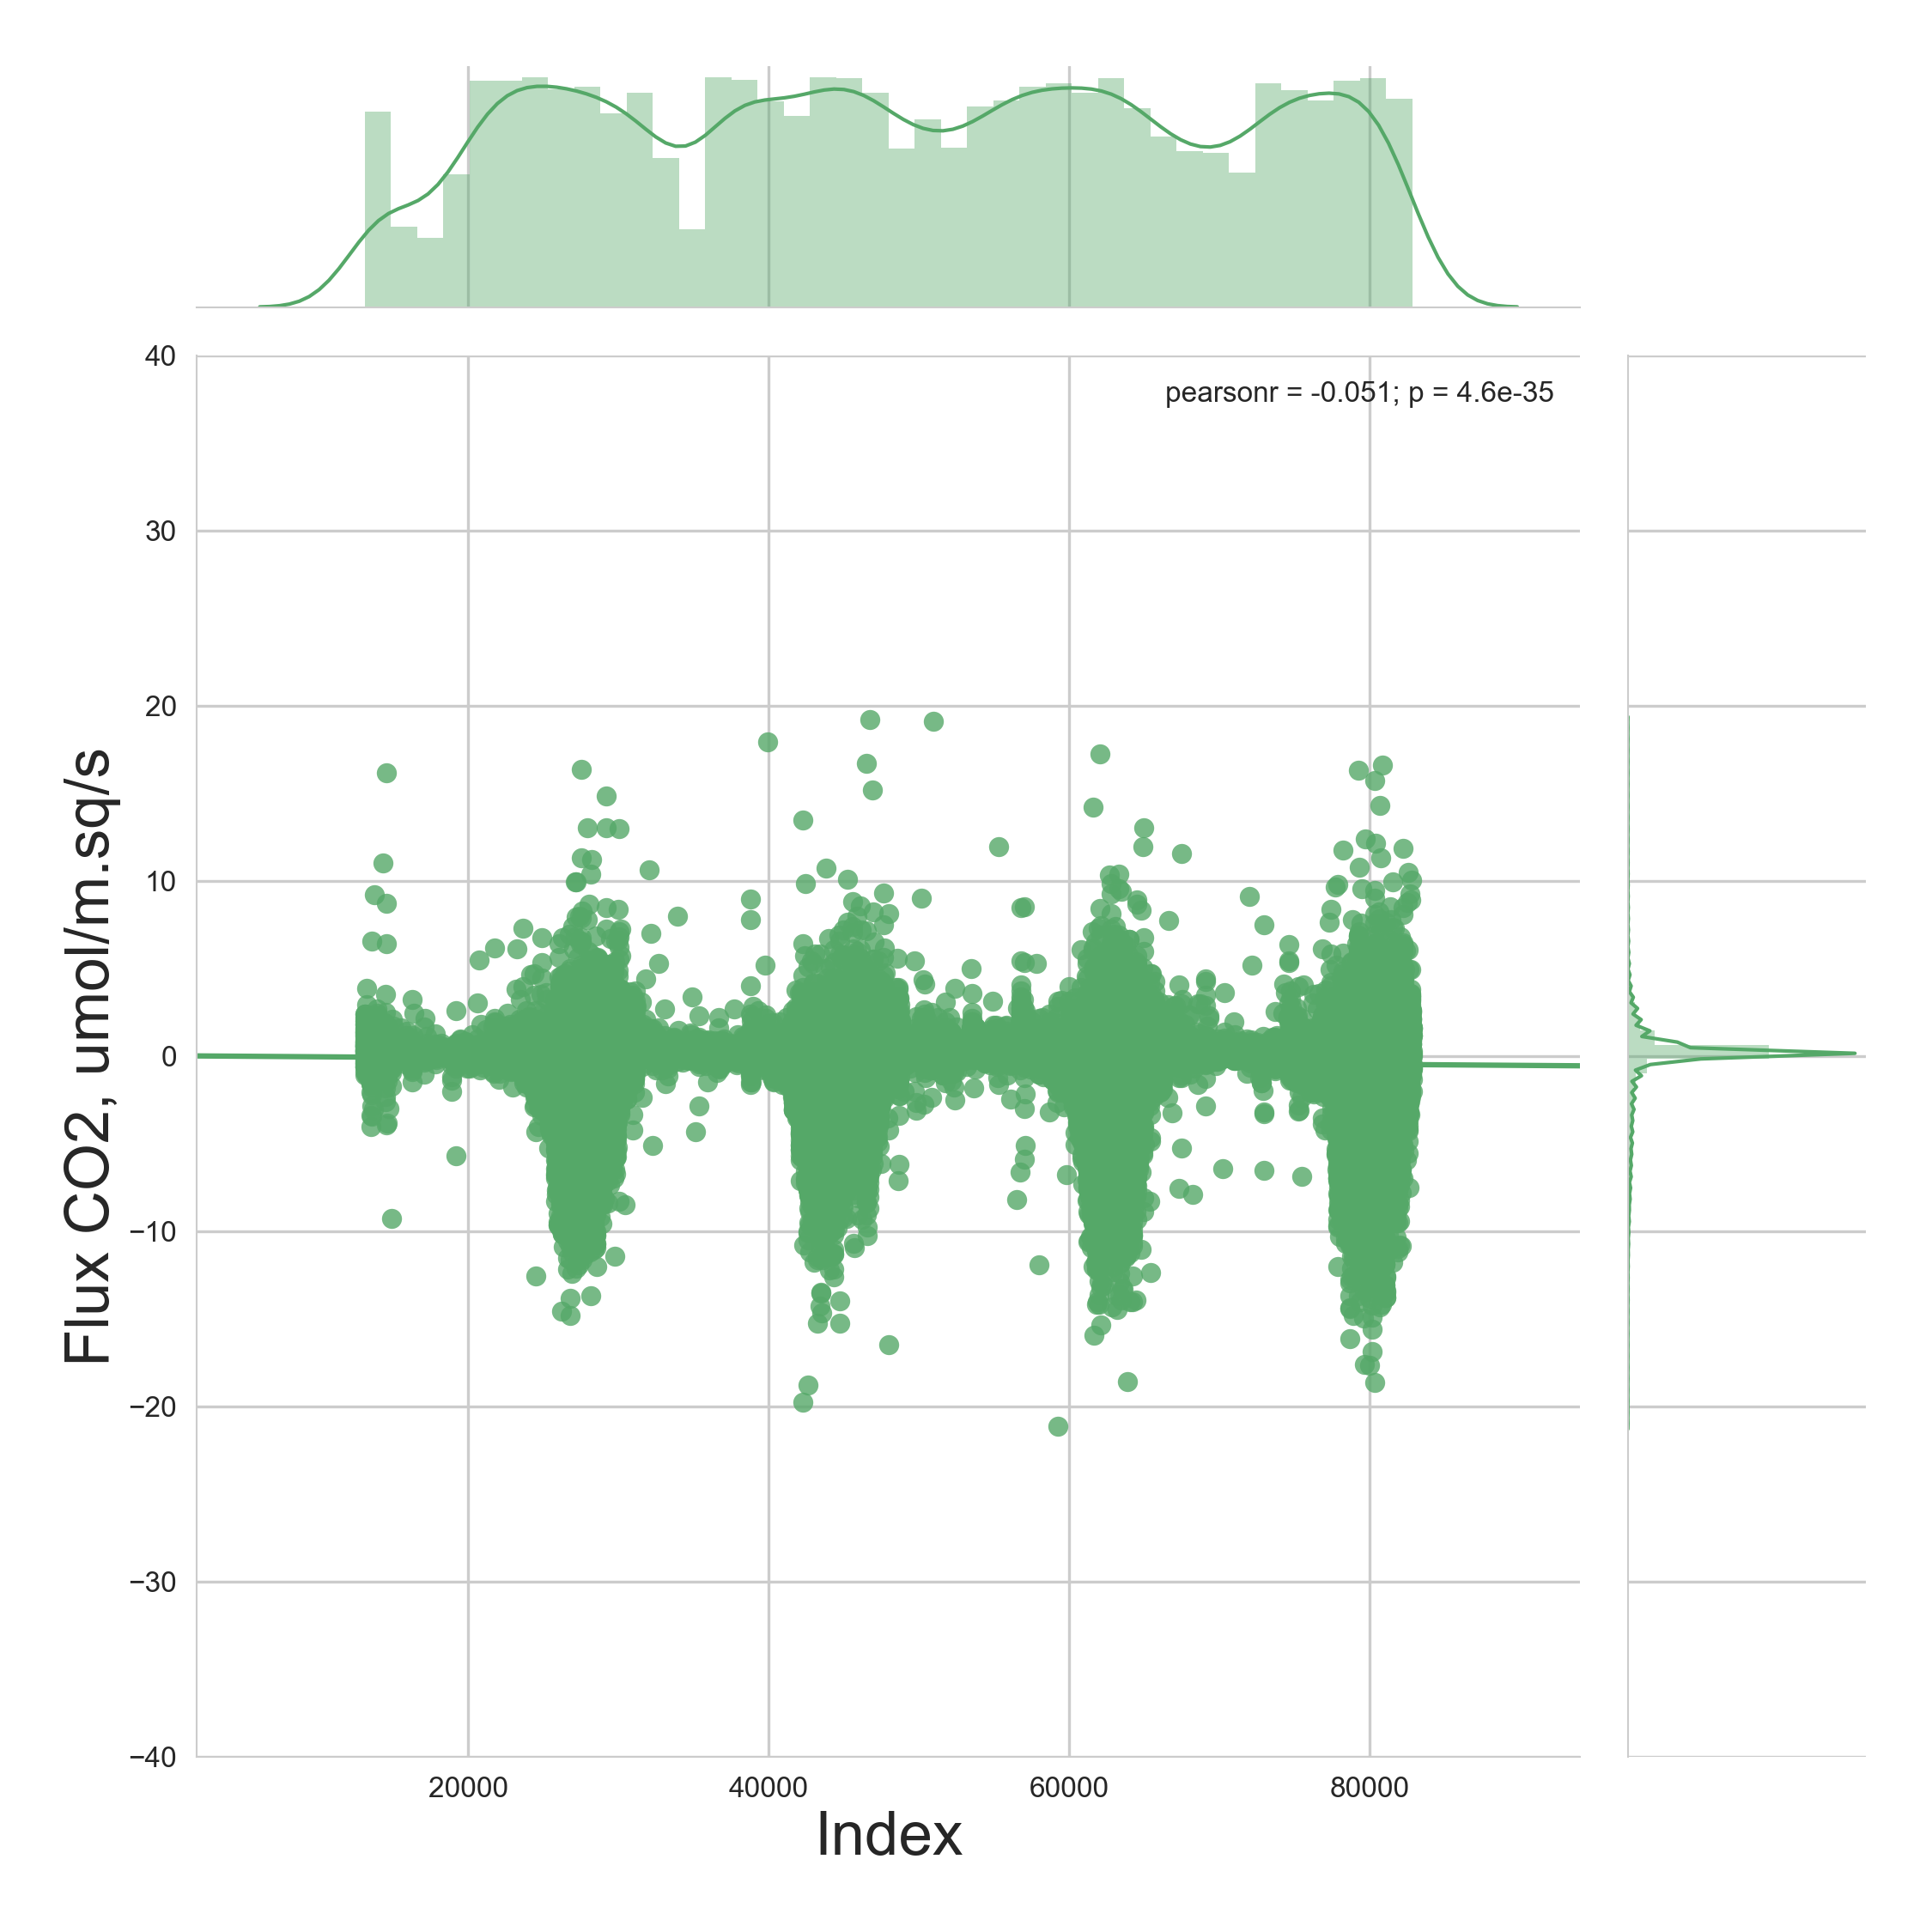
\includegraphics[width=\textwidth]{FvsTimeDen/CA-NS6.png}\\
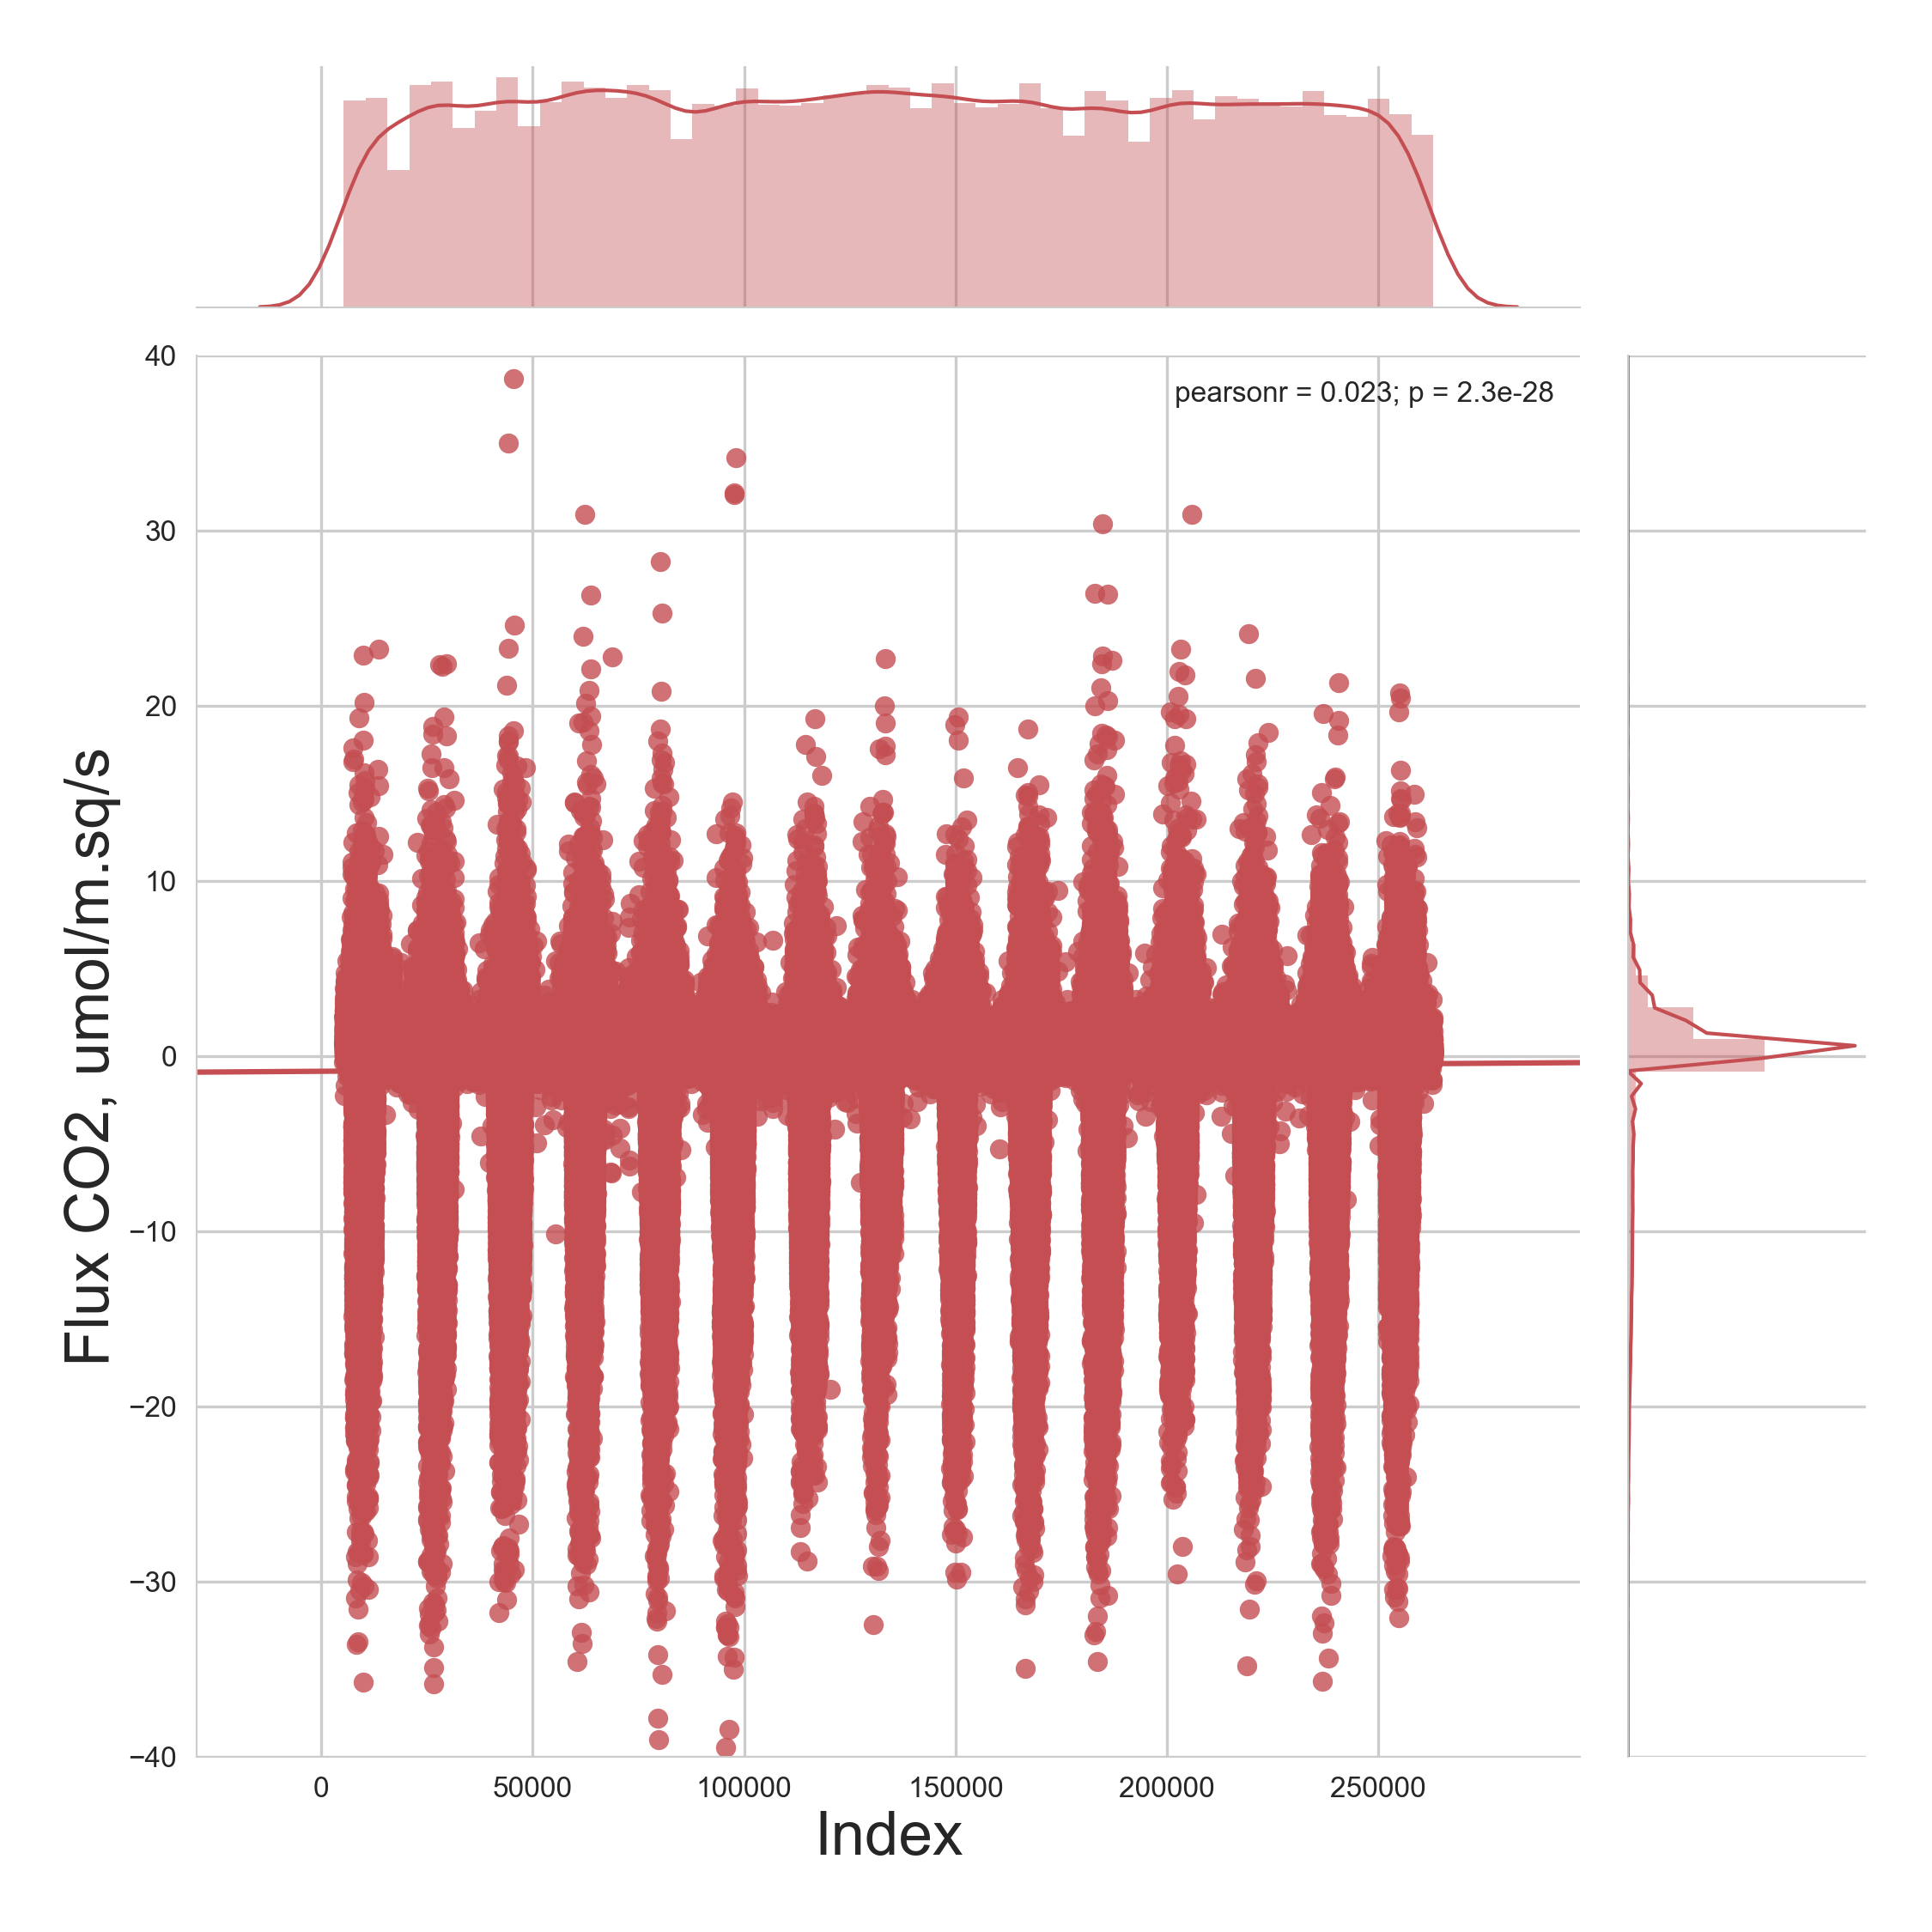
\includegraphics[width=\textwidth]{FvsTimeDen/CA-Oas.png}
\column{.35\textwidth}
\centering
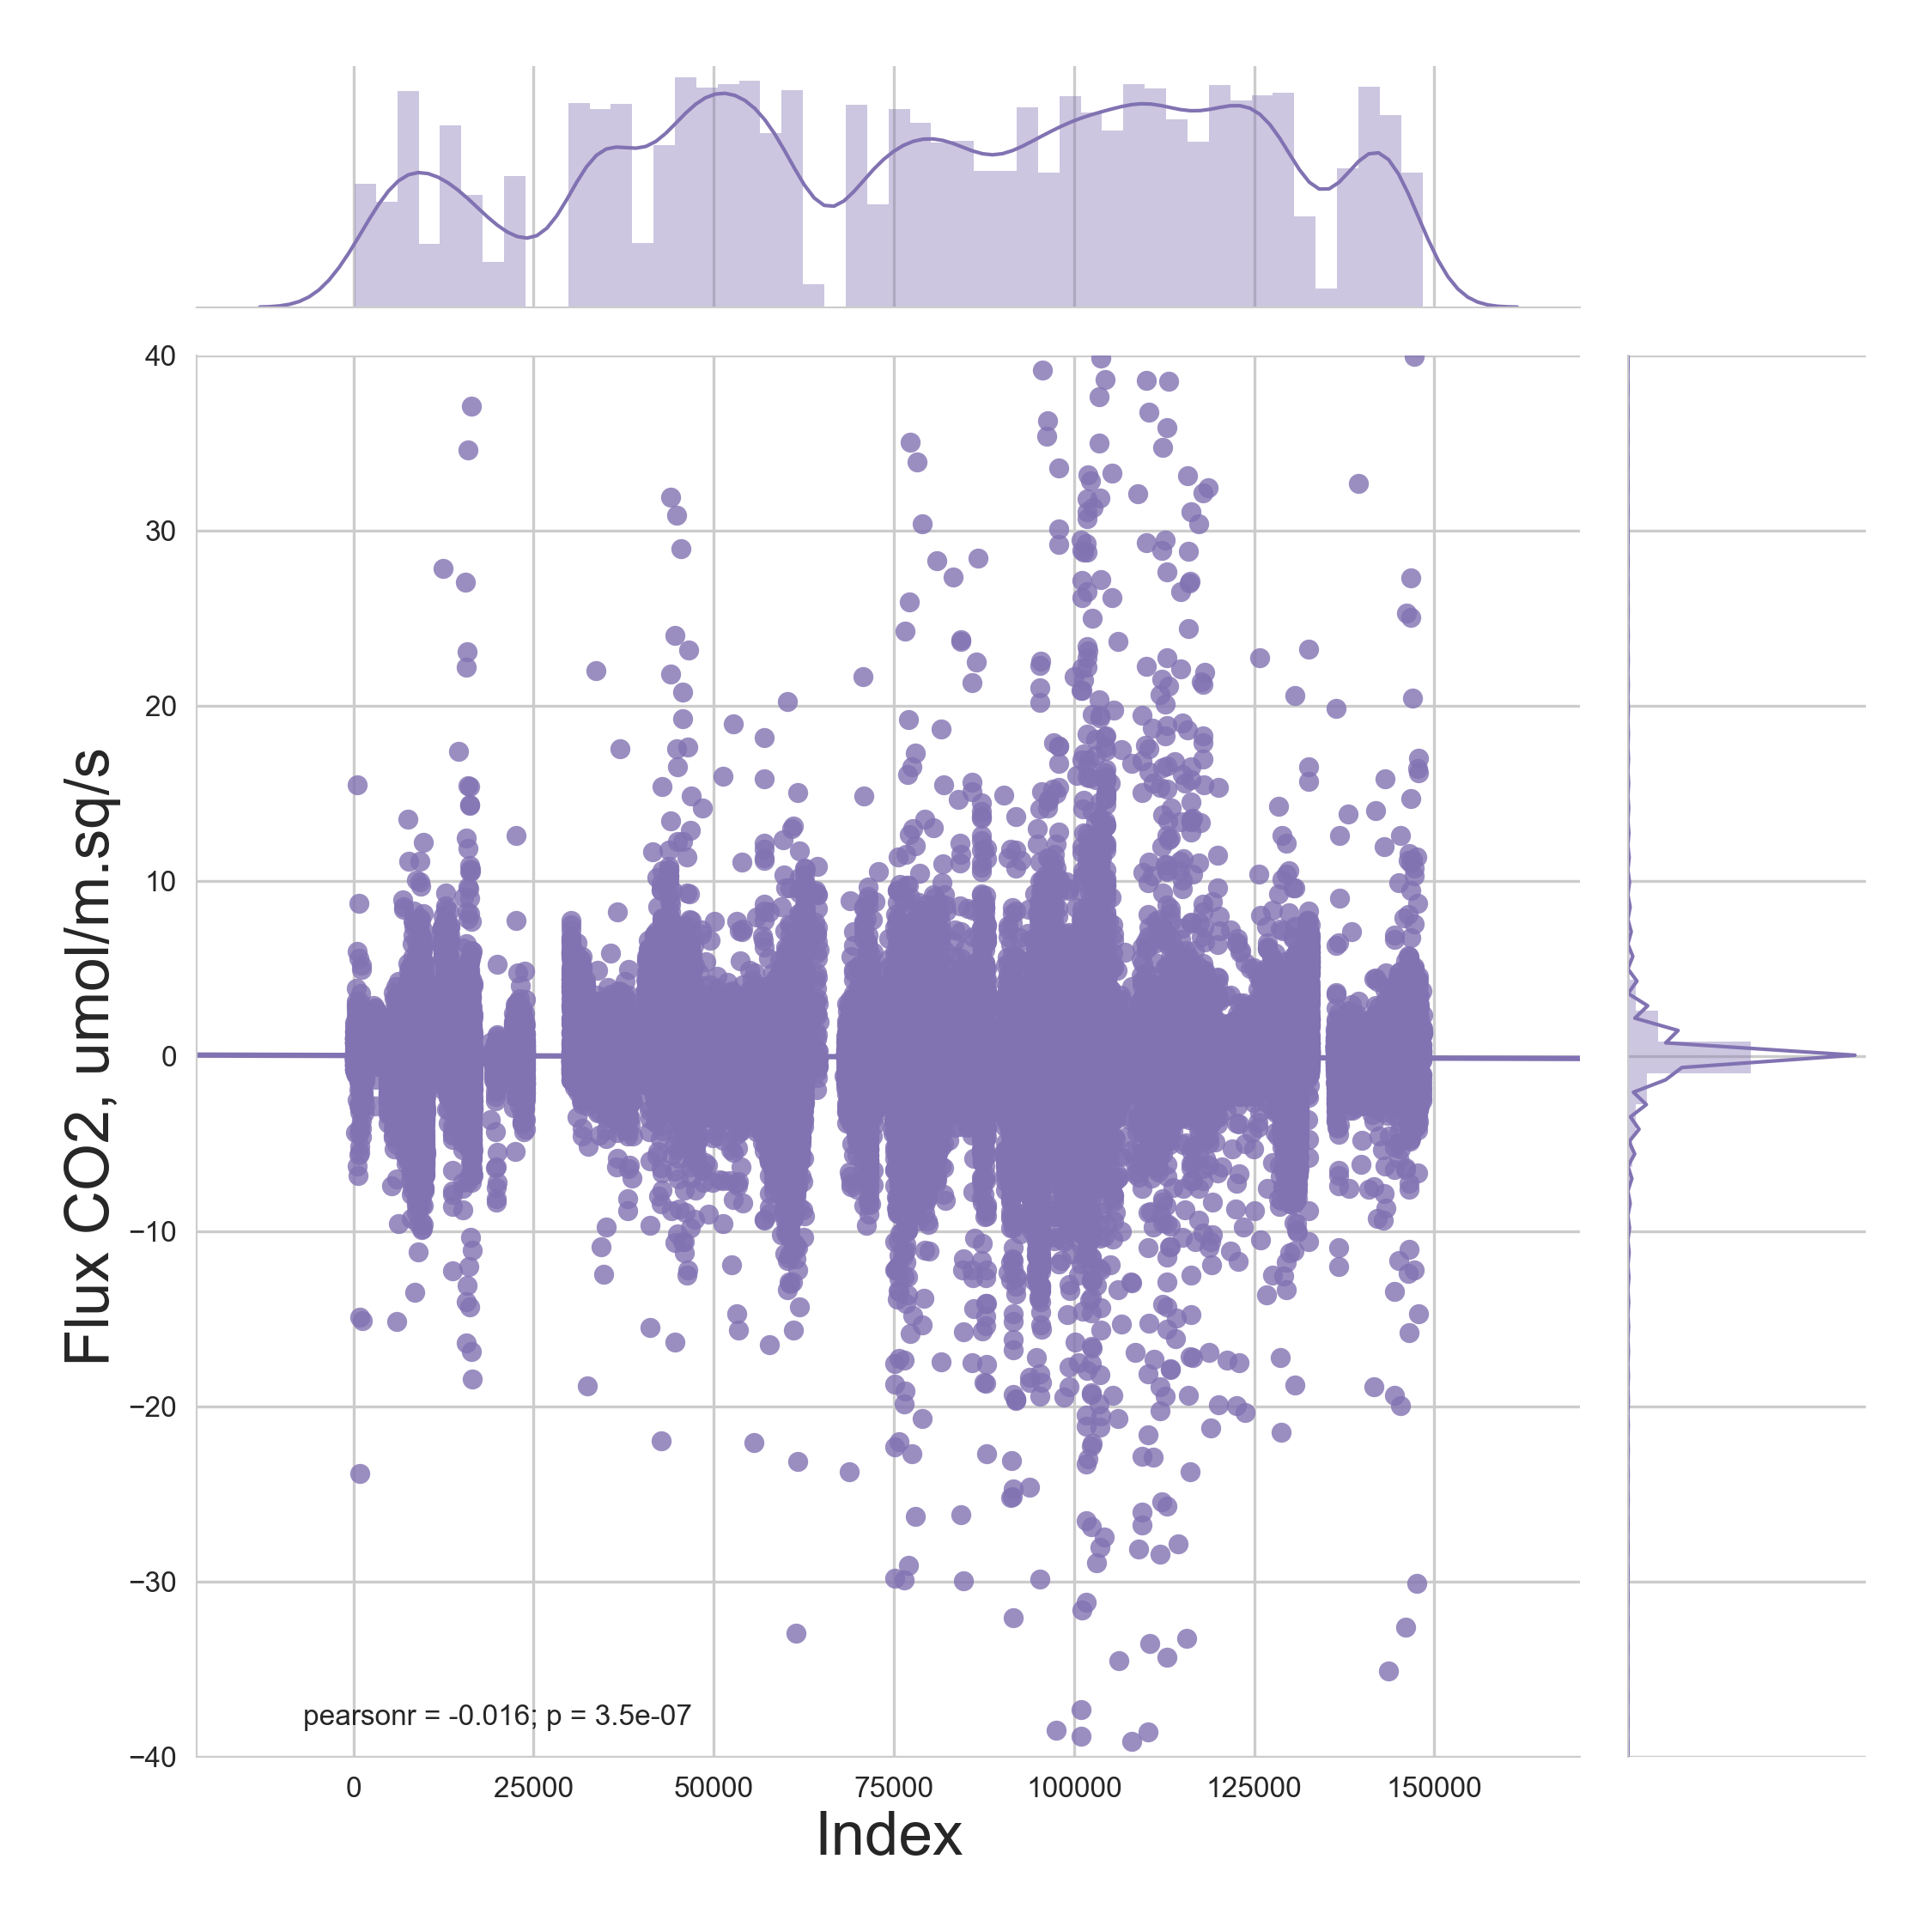
\includegraphics[width=\textwidth]{FvsTimeDen/US-FPe.png}\\
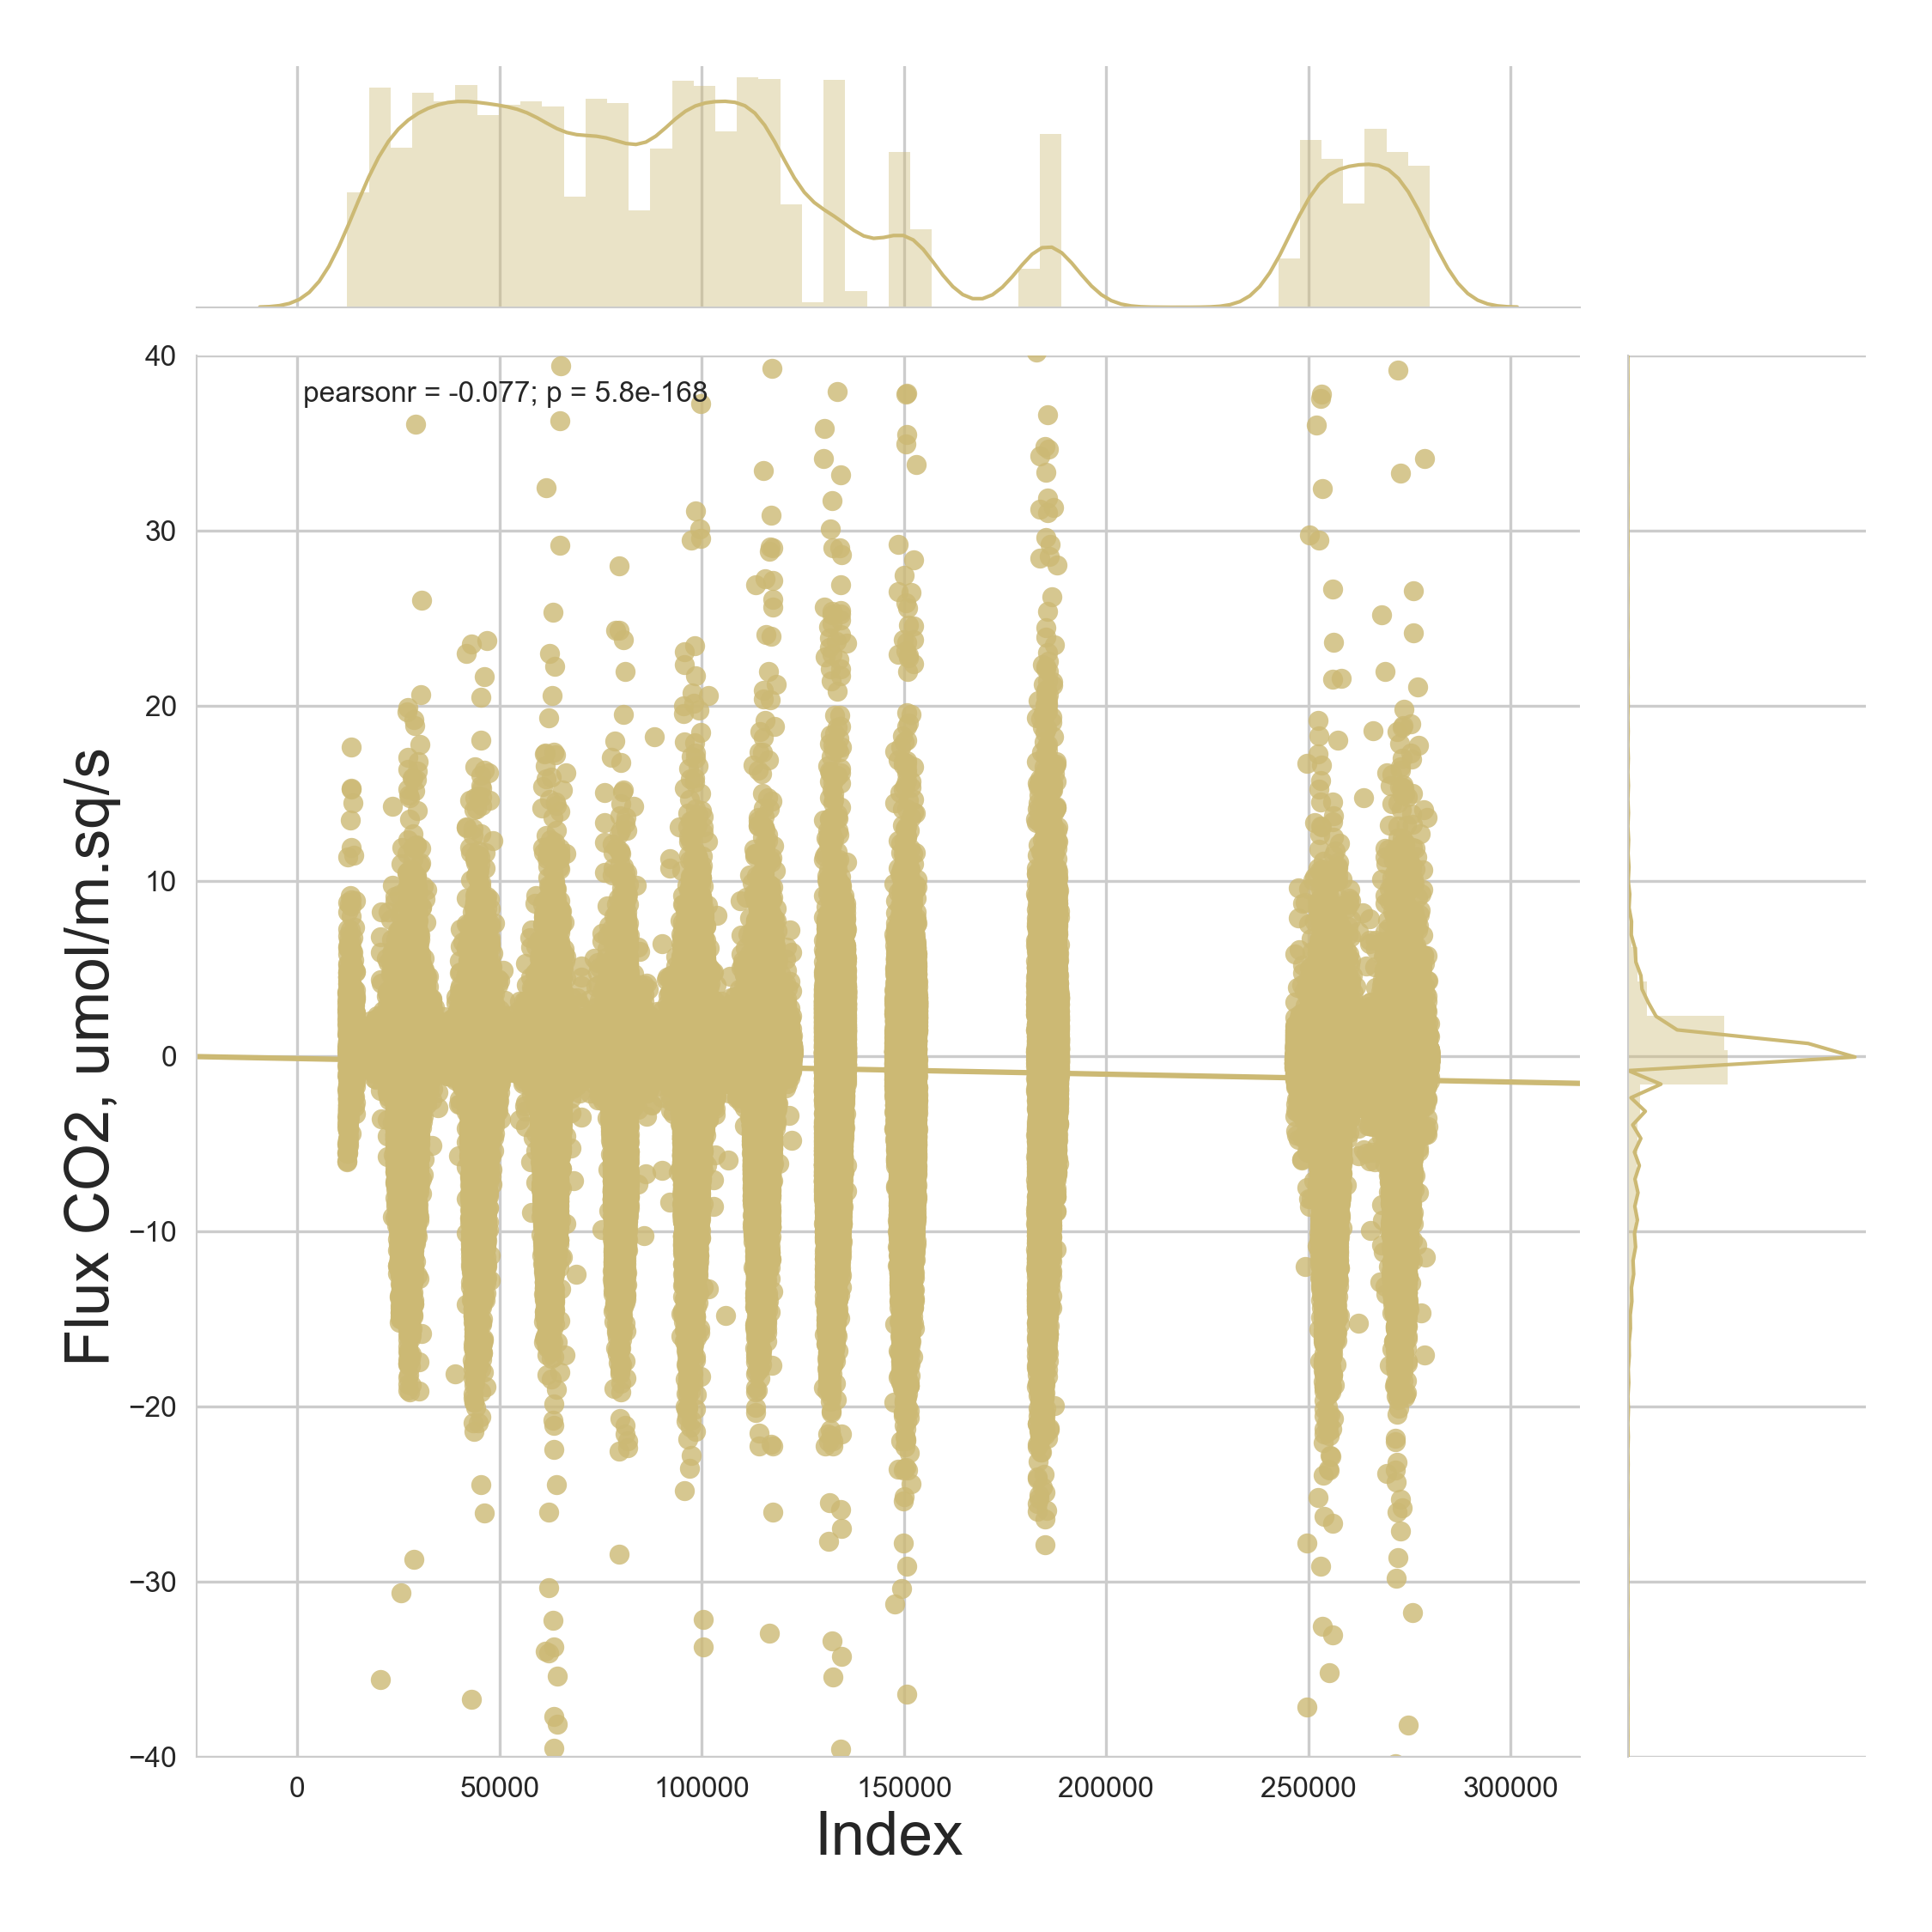
\includegraphics[width=\textwidth]{FvsTimeDen/US-Los.png}
\end{columns}

\end{frame}

\begin{frame}
\frametitle{Flux vs Soil Temperature}

\begin{columns}[t]
\column{.35\textwidth}
\centering
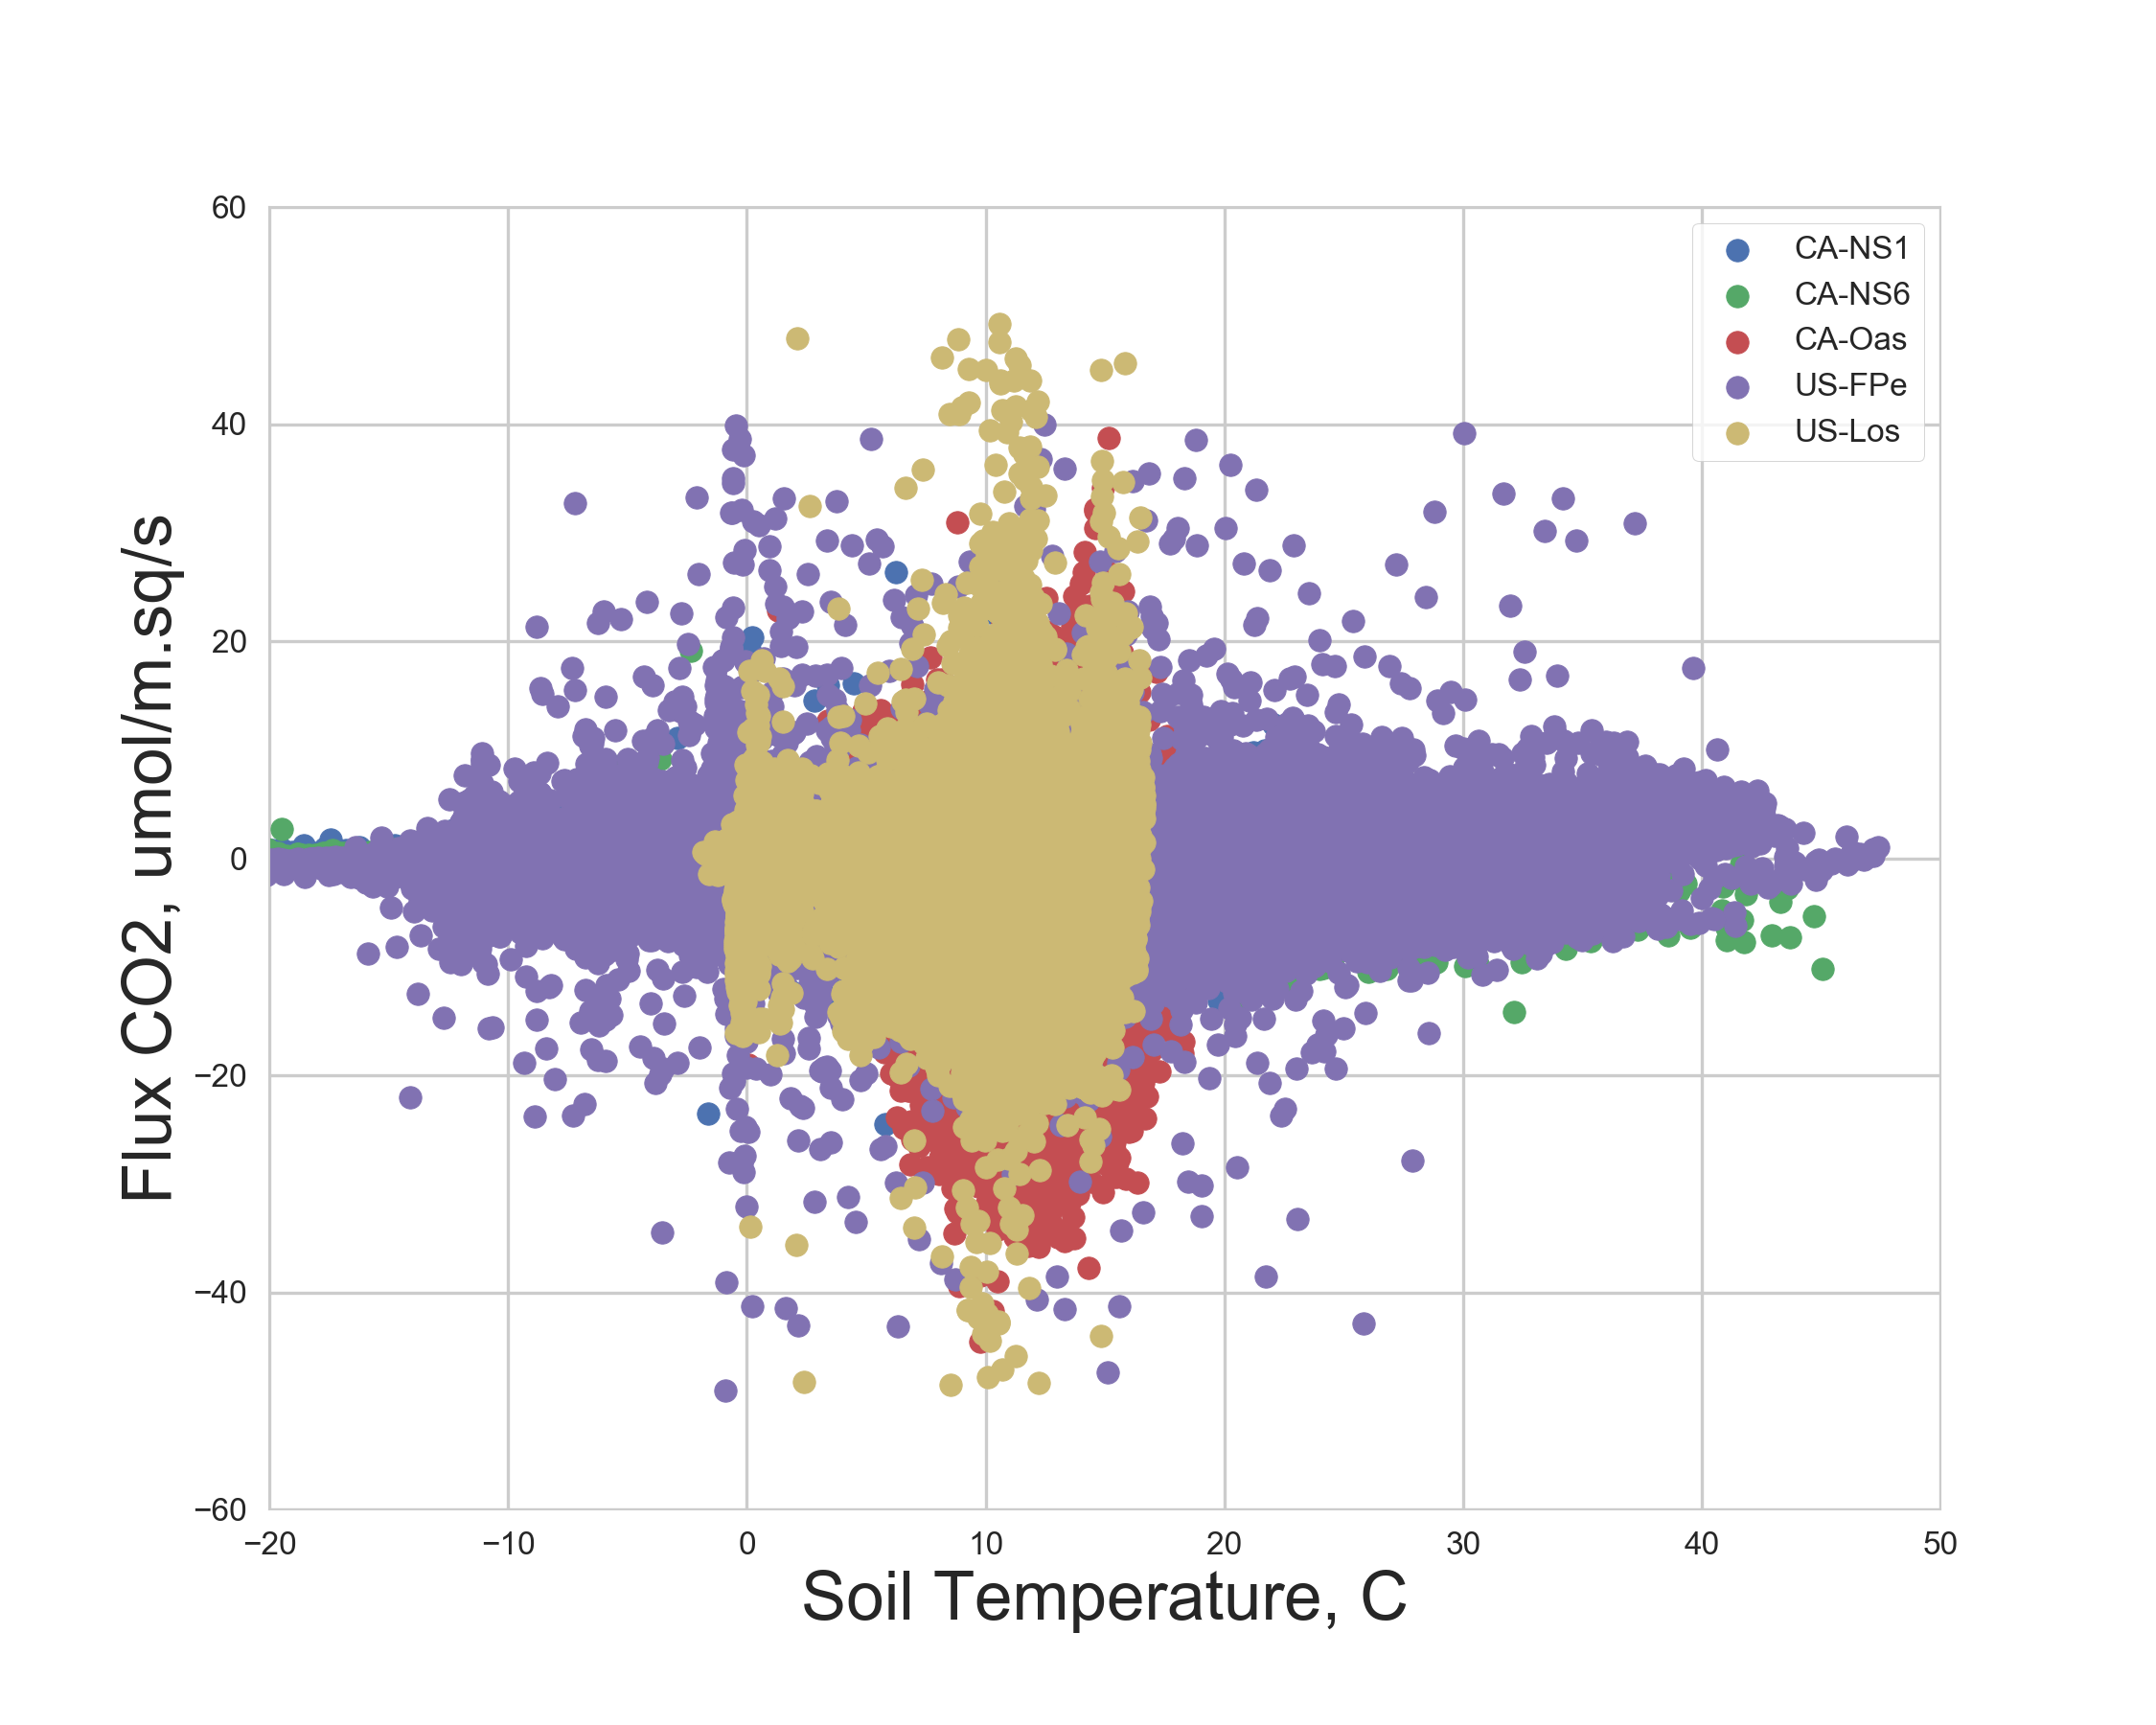
\includegraphics[width=\textwidth]{FvsT/all.png}\\
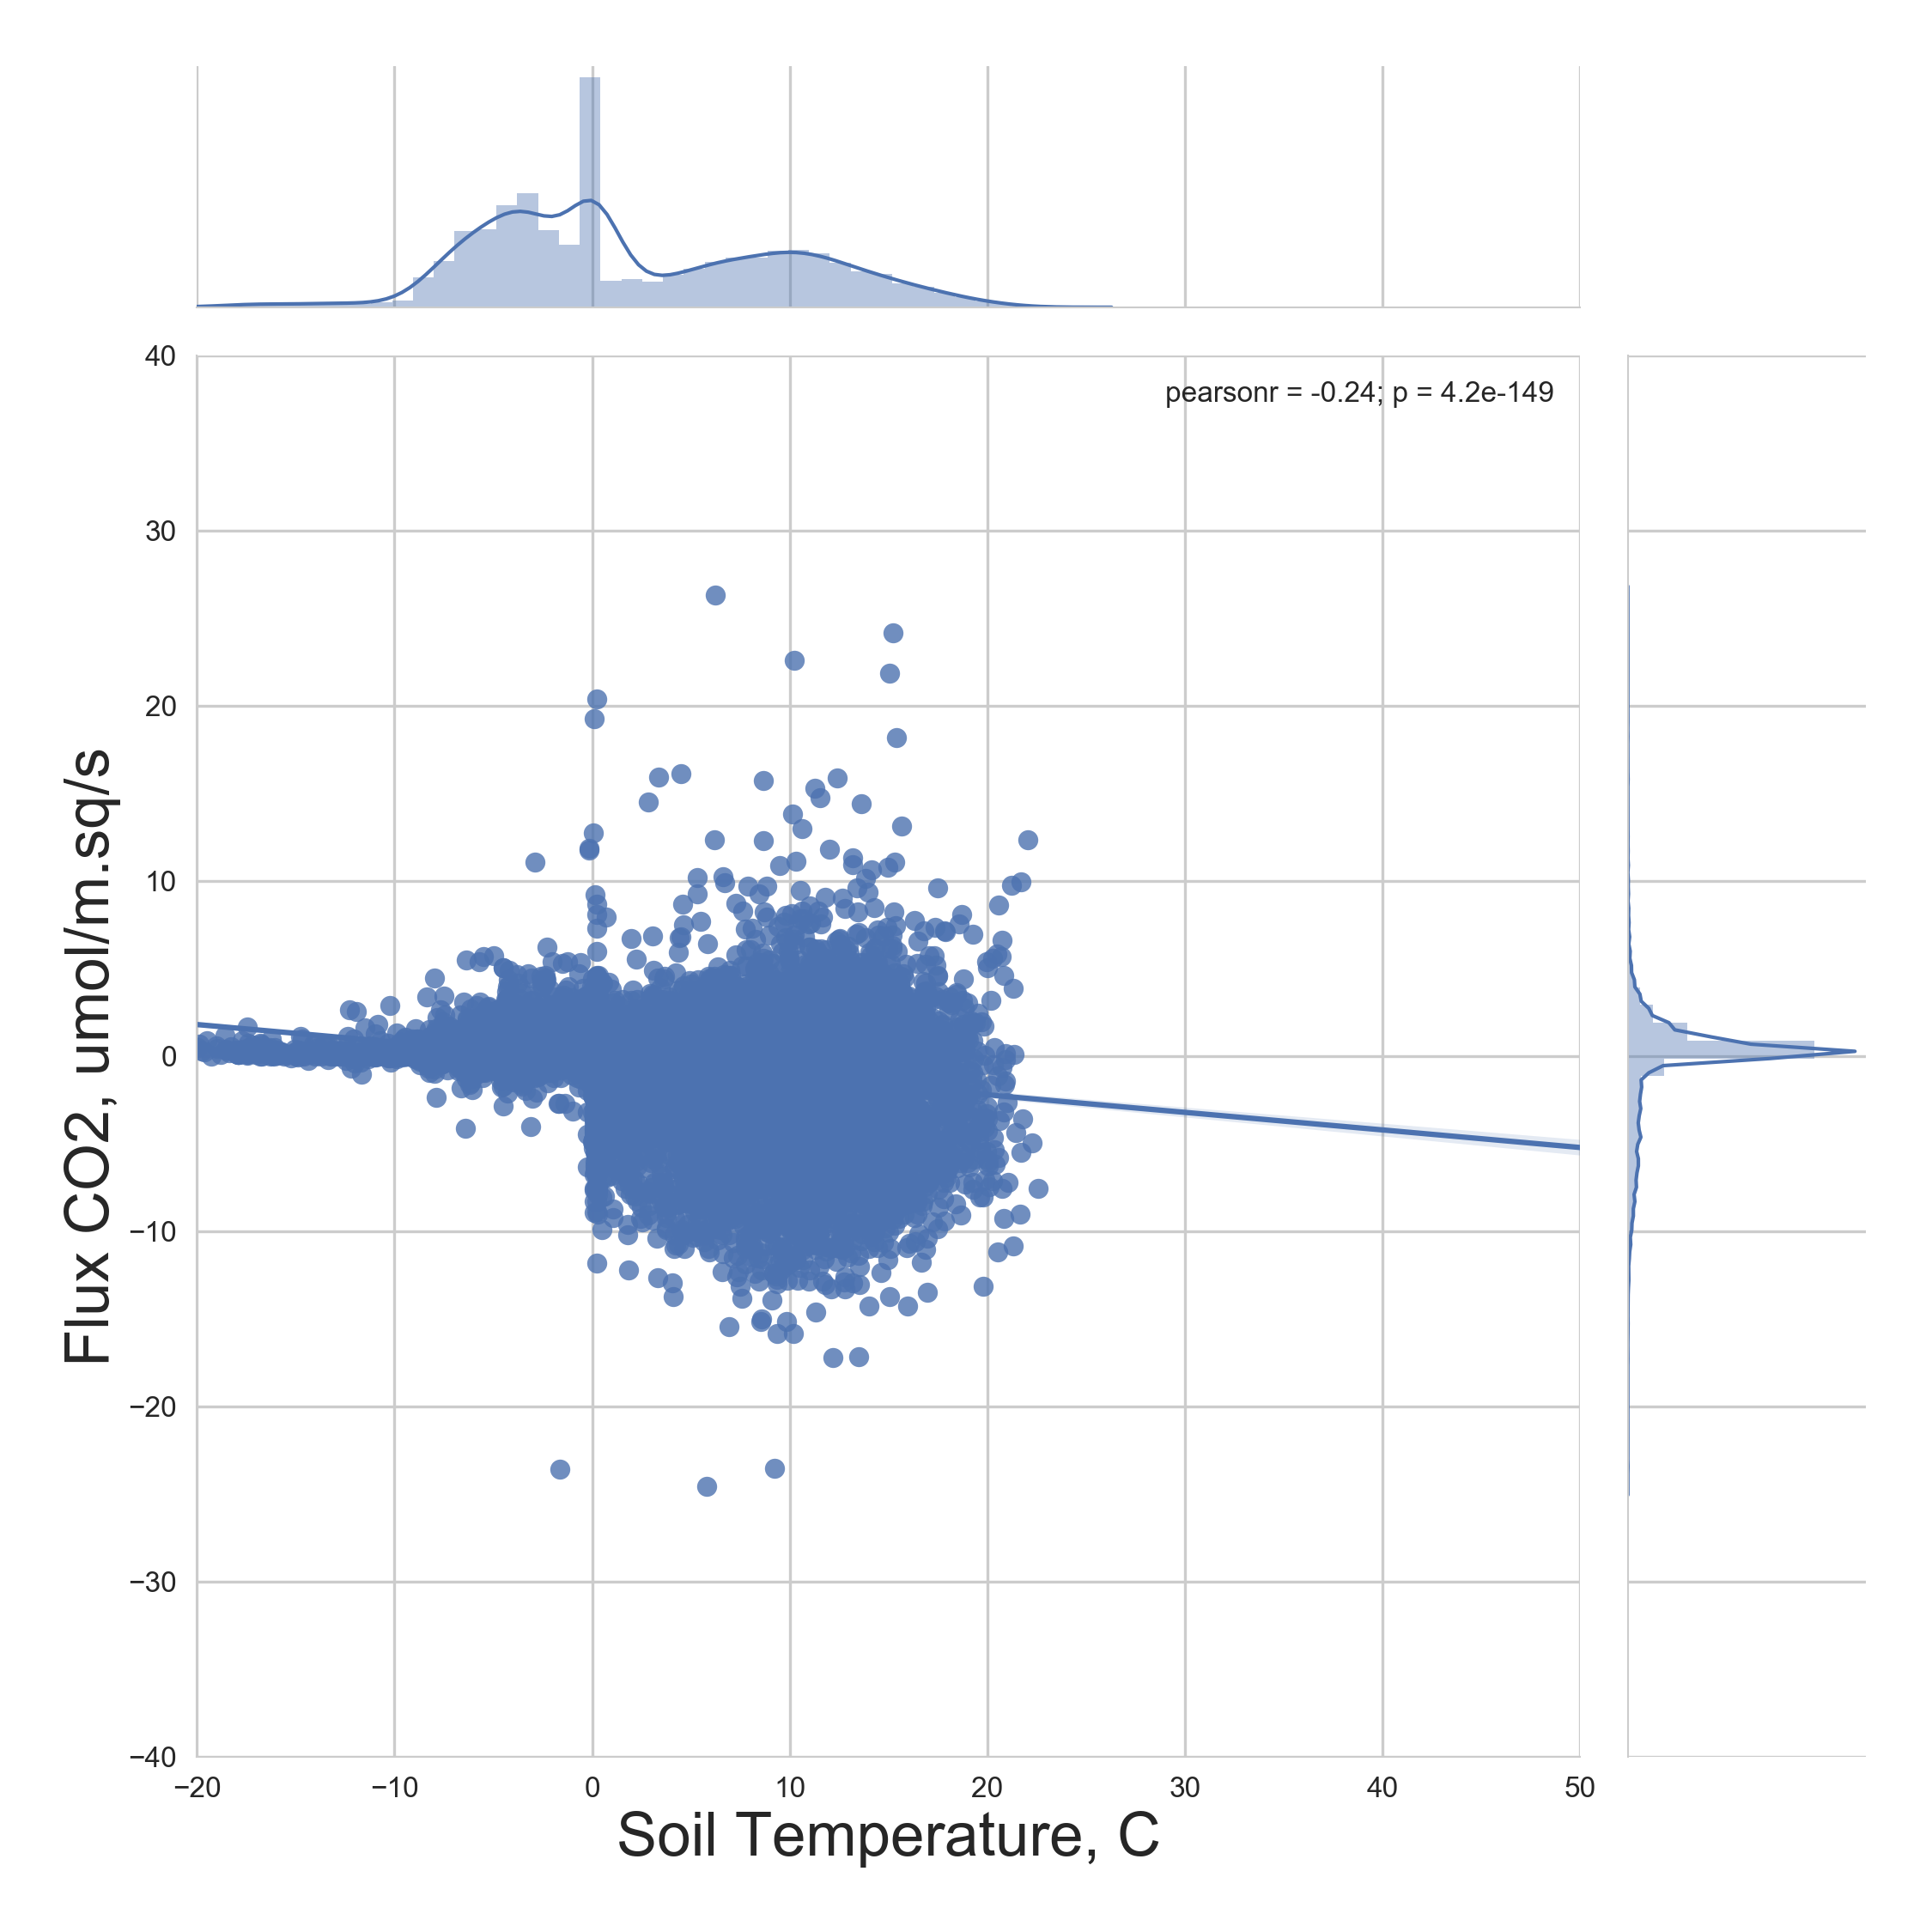
\includegraphics[width=\textwidth]{FvsT/CA-NS1.png}
\column{.35\textwidth}
\centering
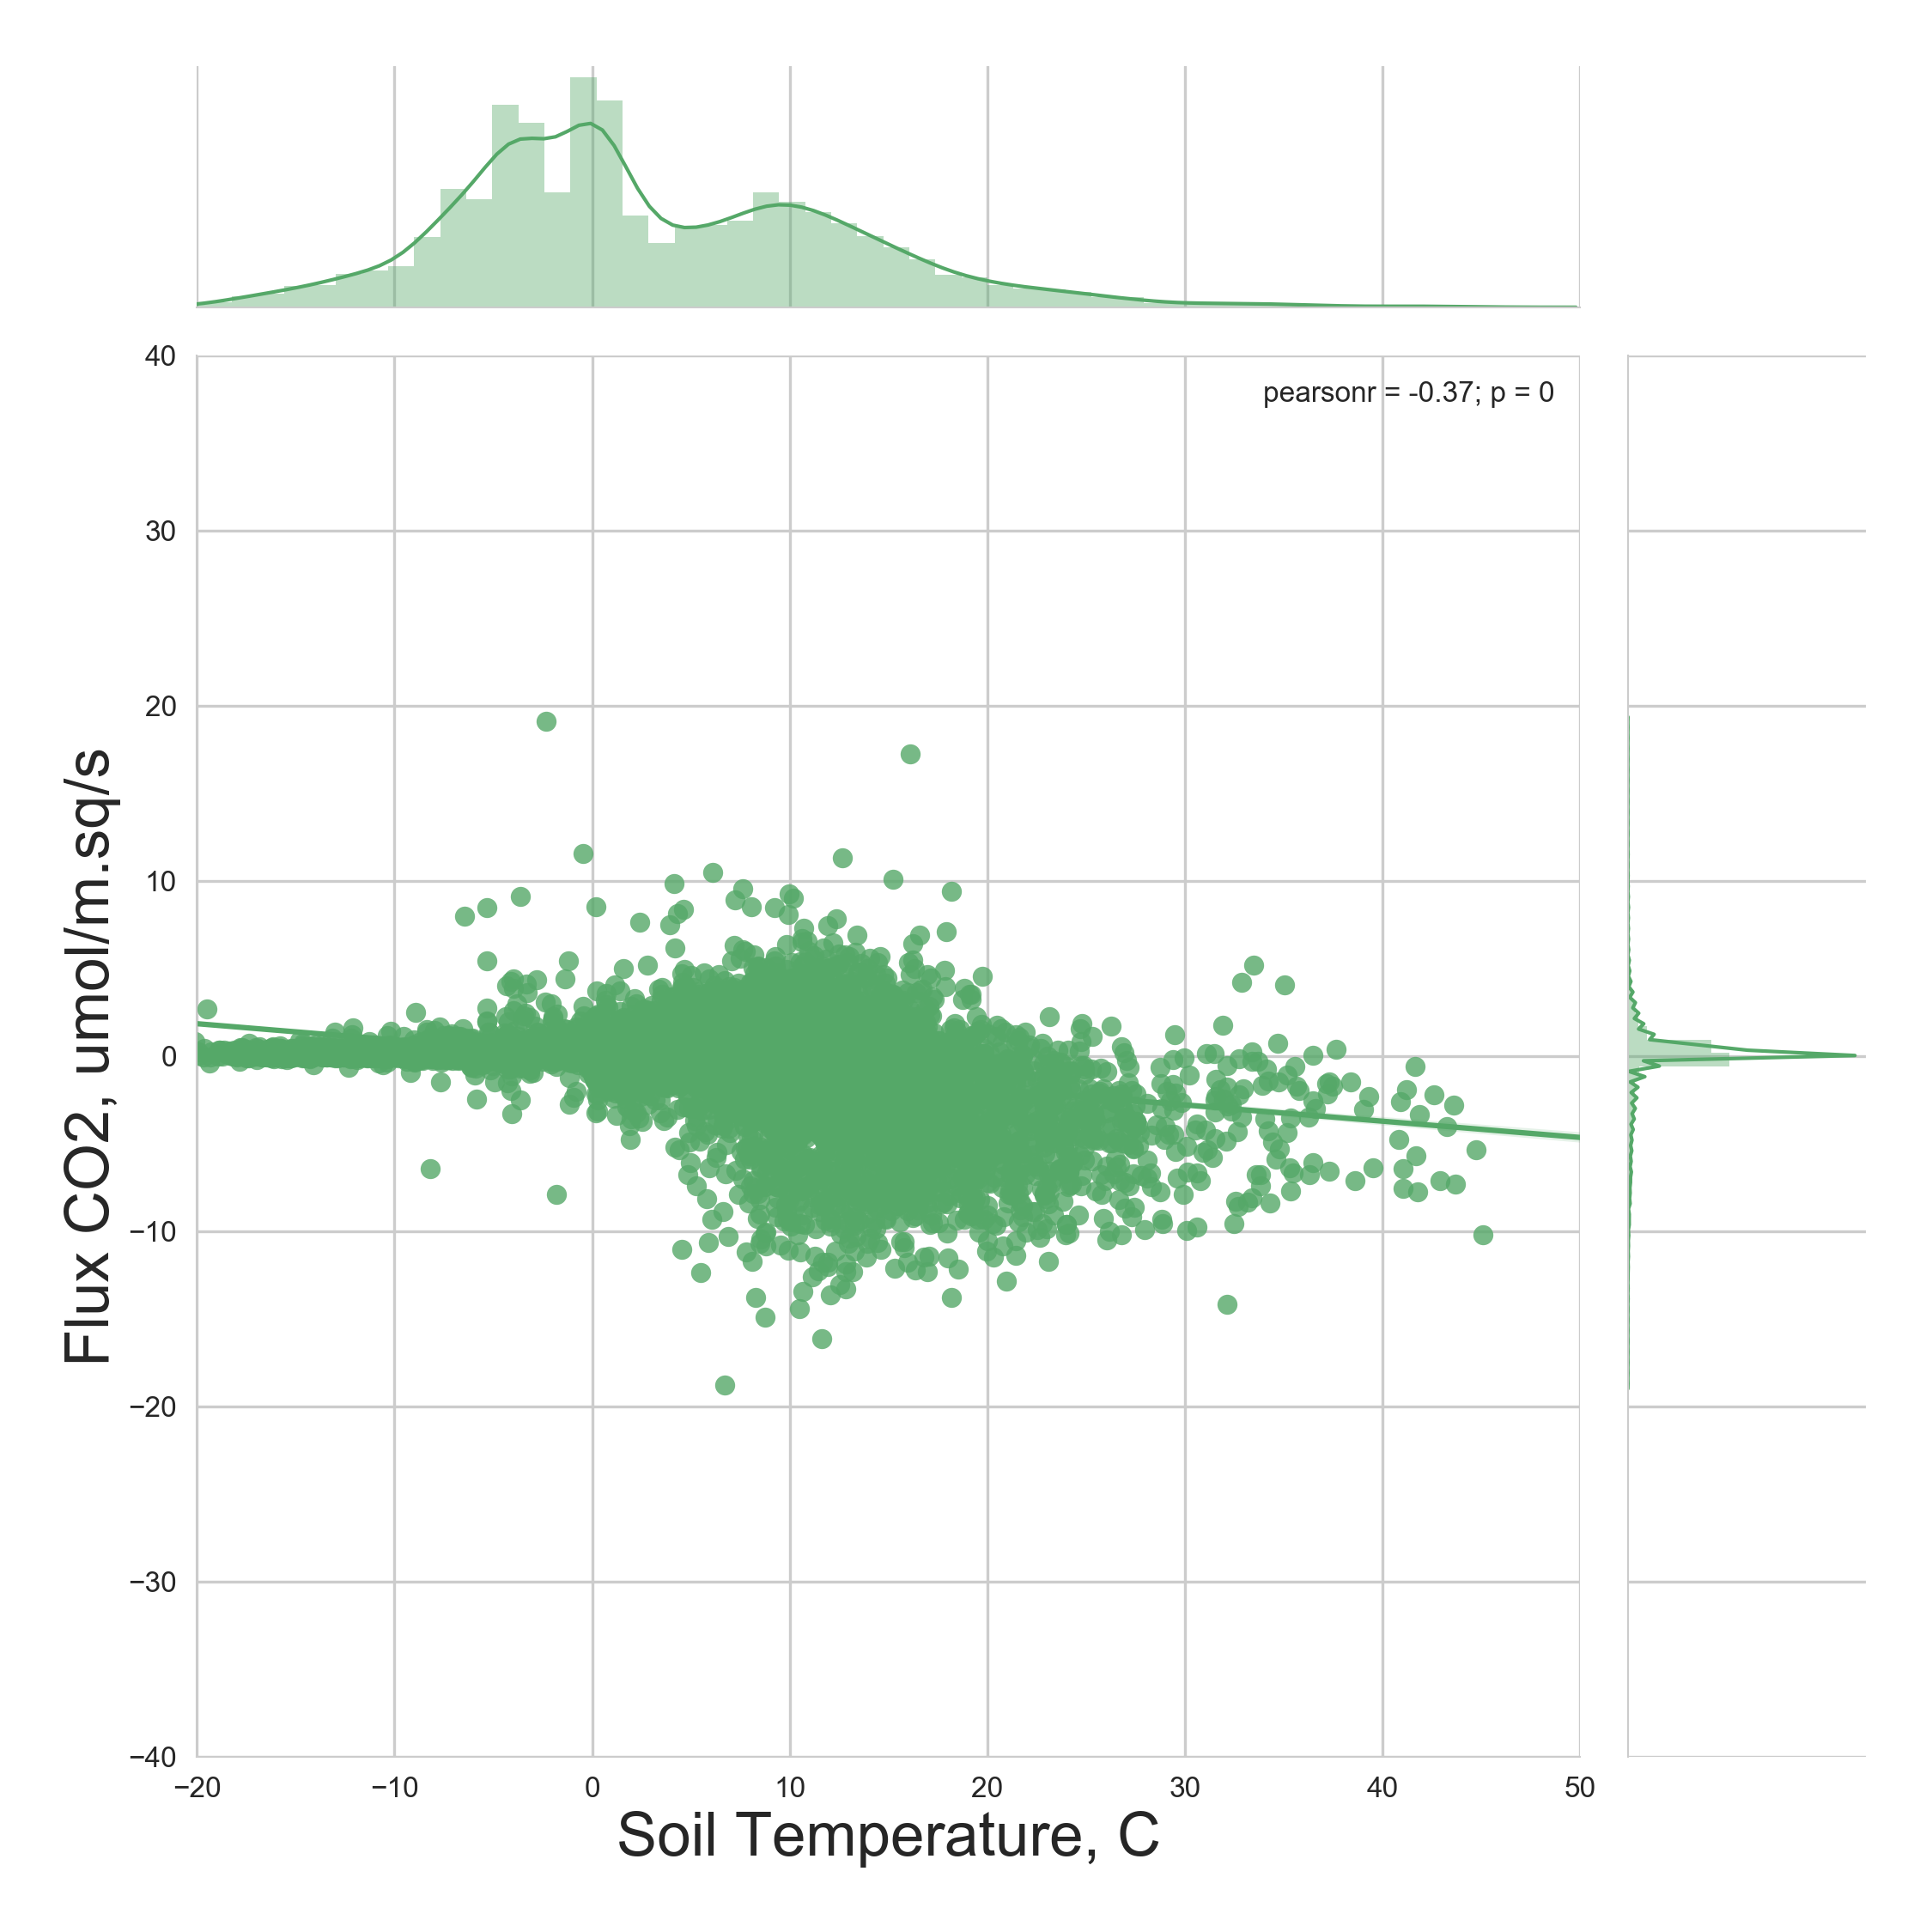
\includegraphics[width=\textwidth]{FvsT/CA-NS6.png}\\
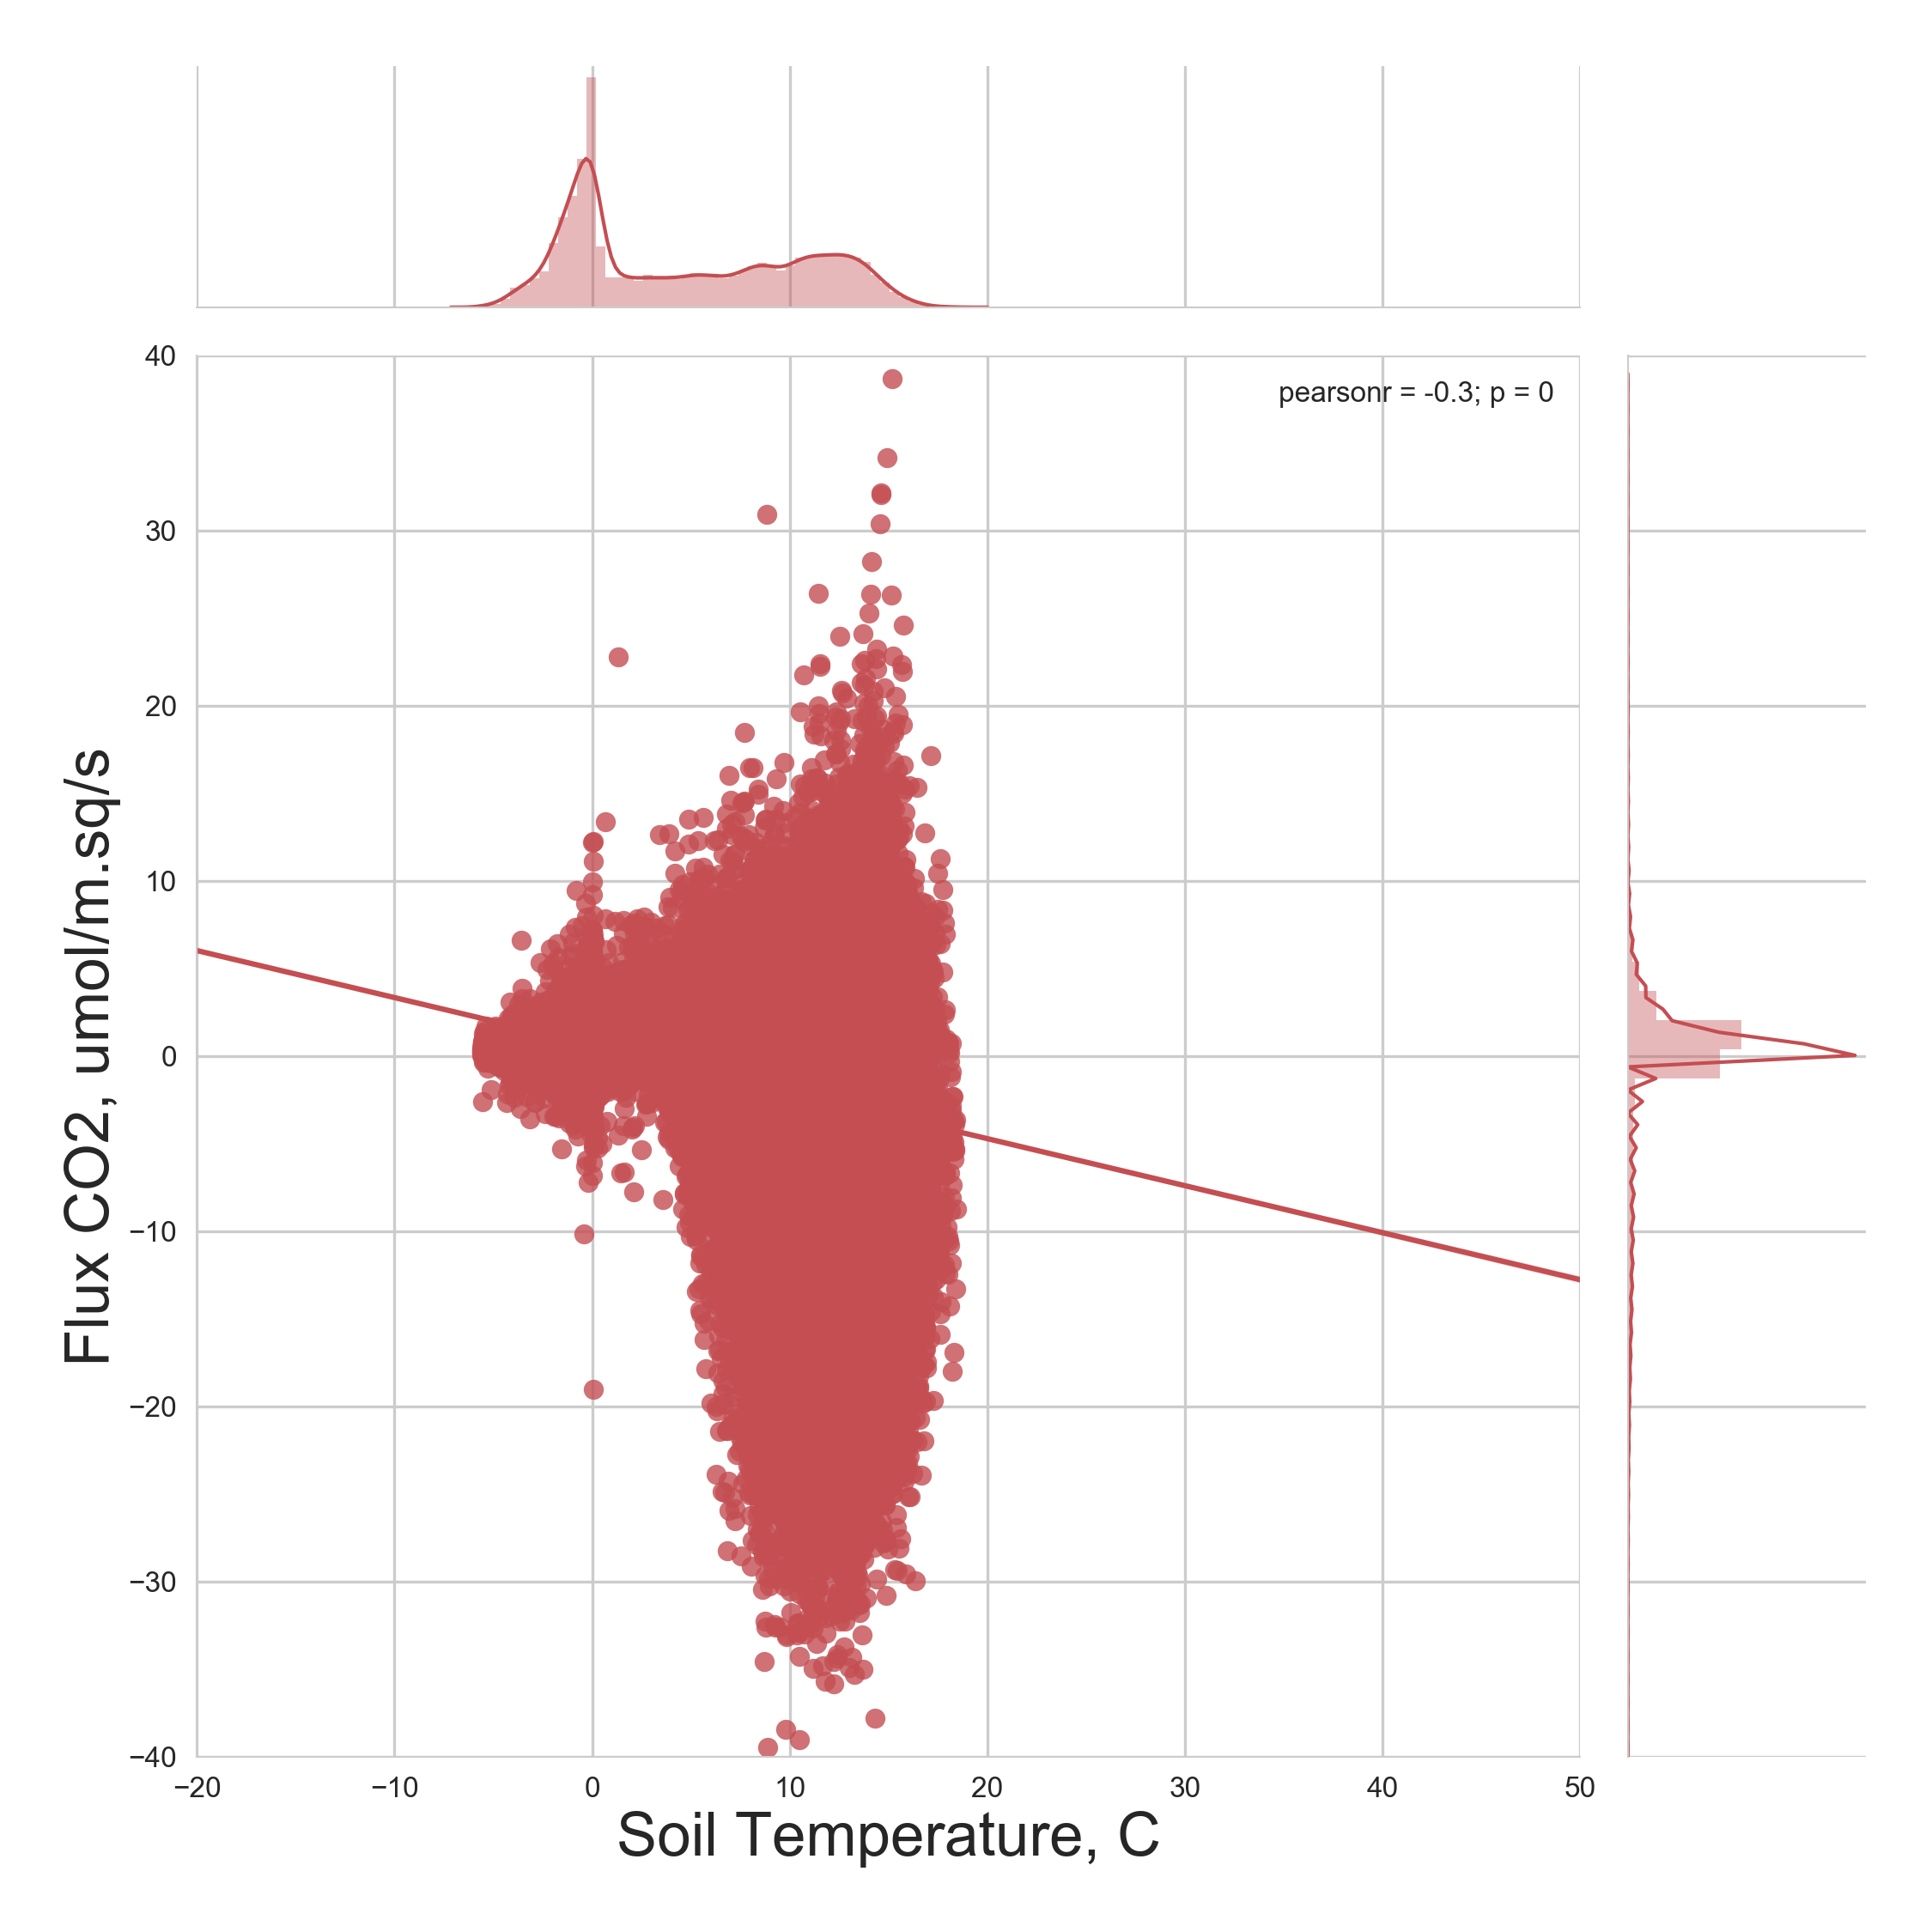
\includegraphics[width=\textwidth]{FvsT/CA-Oas.png}
\column{.35\textwidth}
\centering
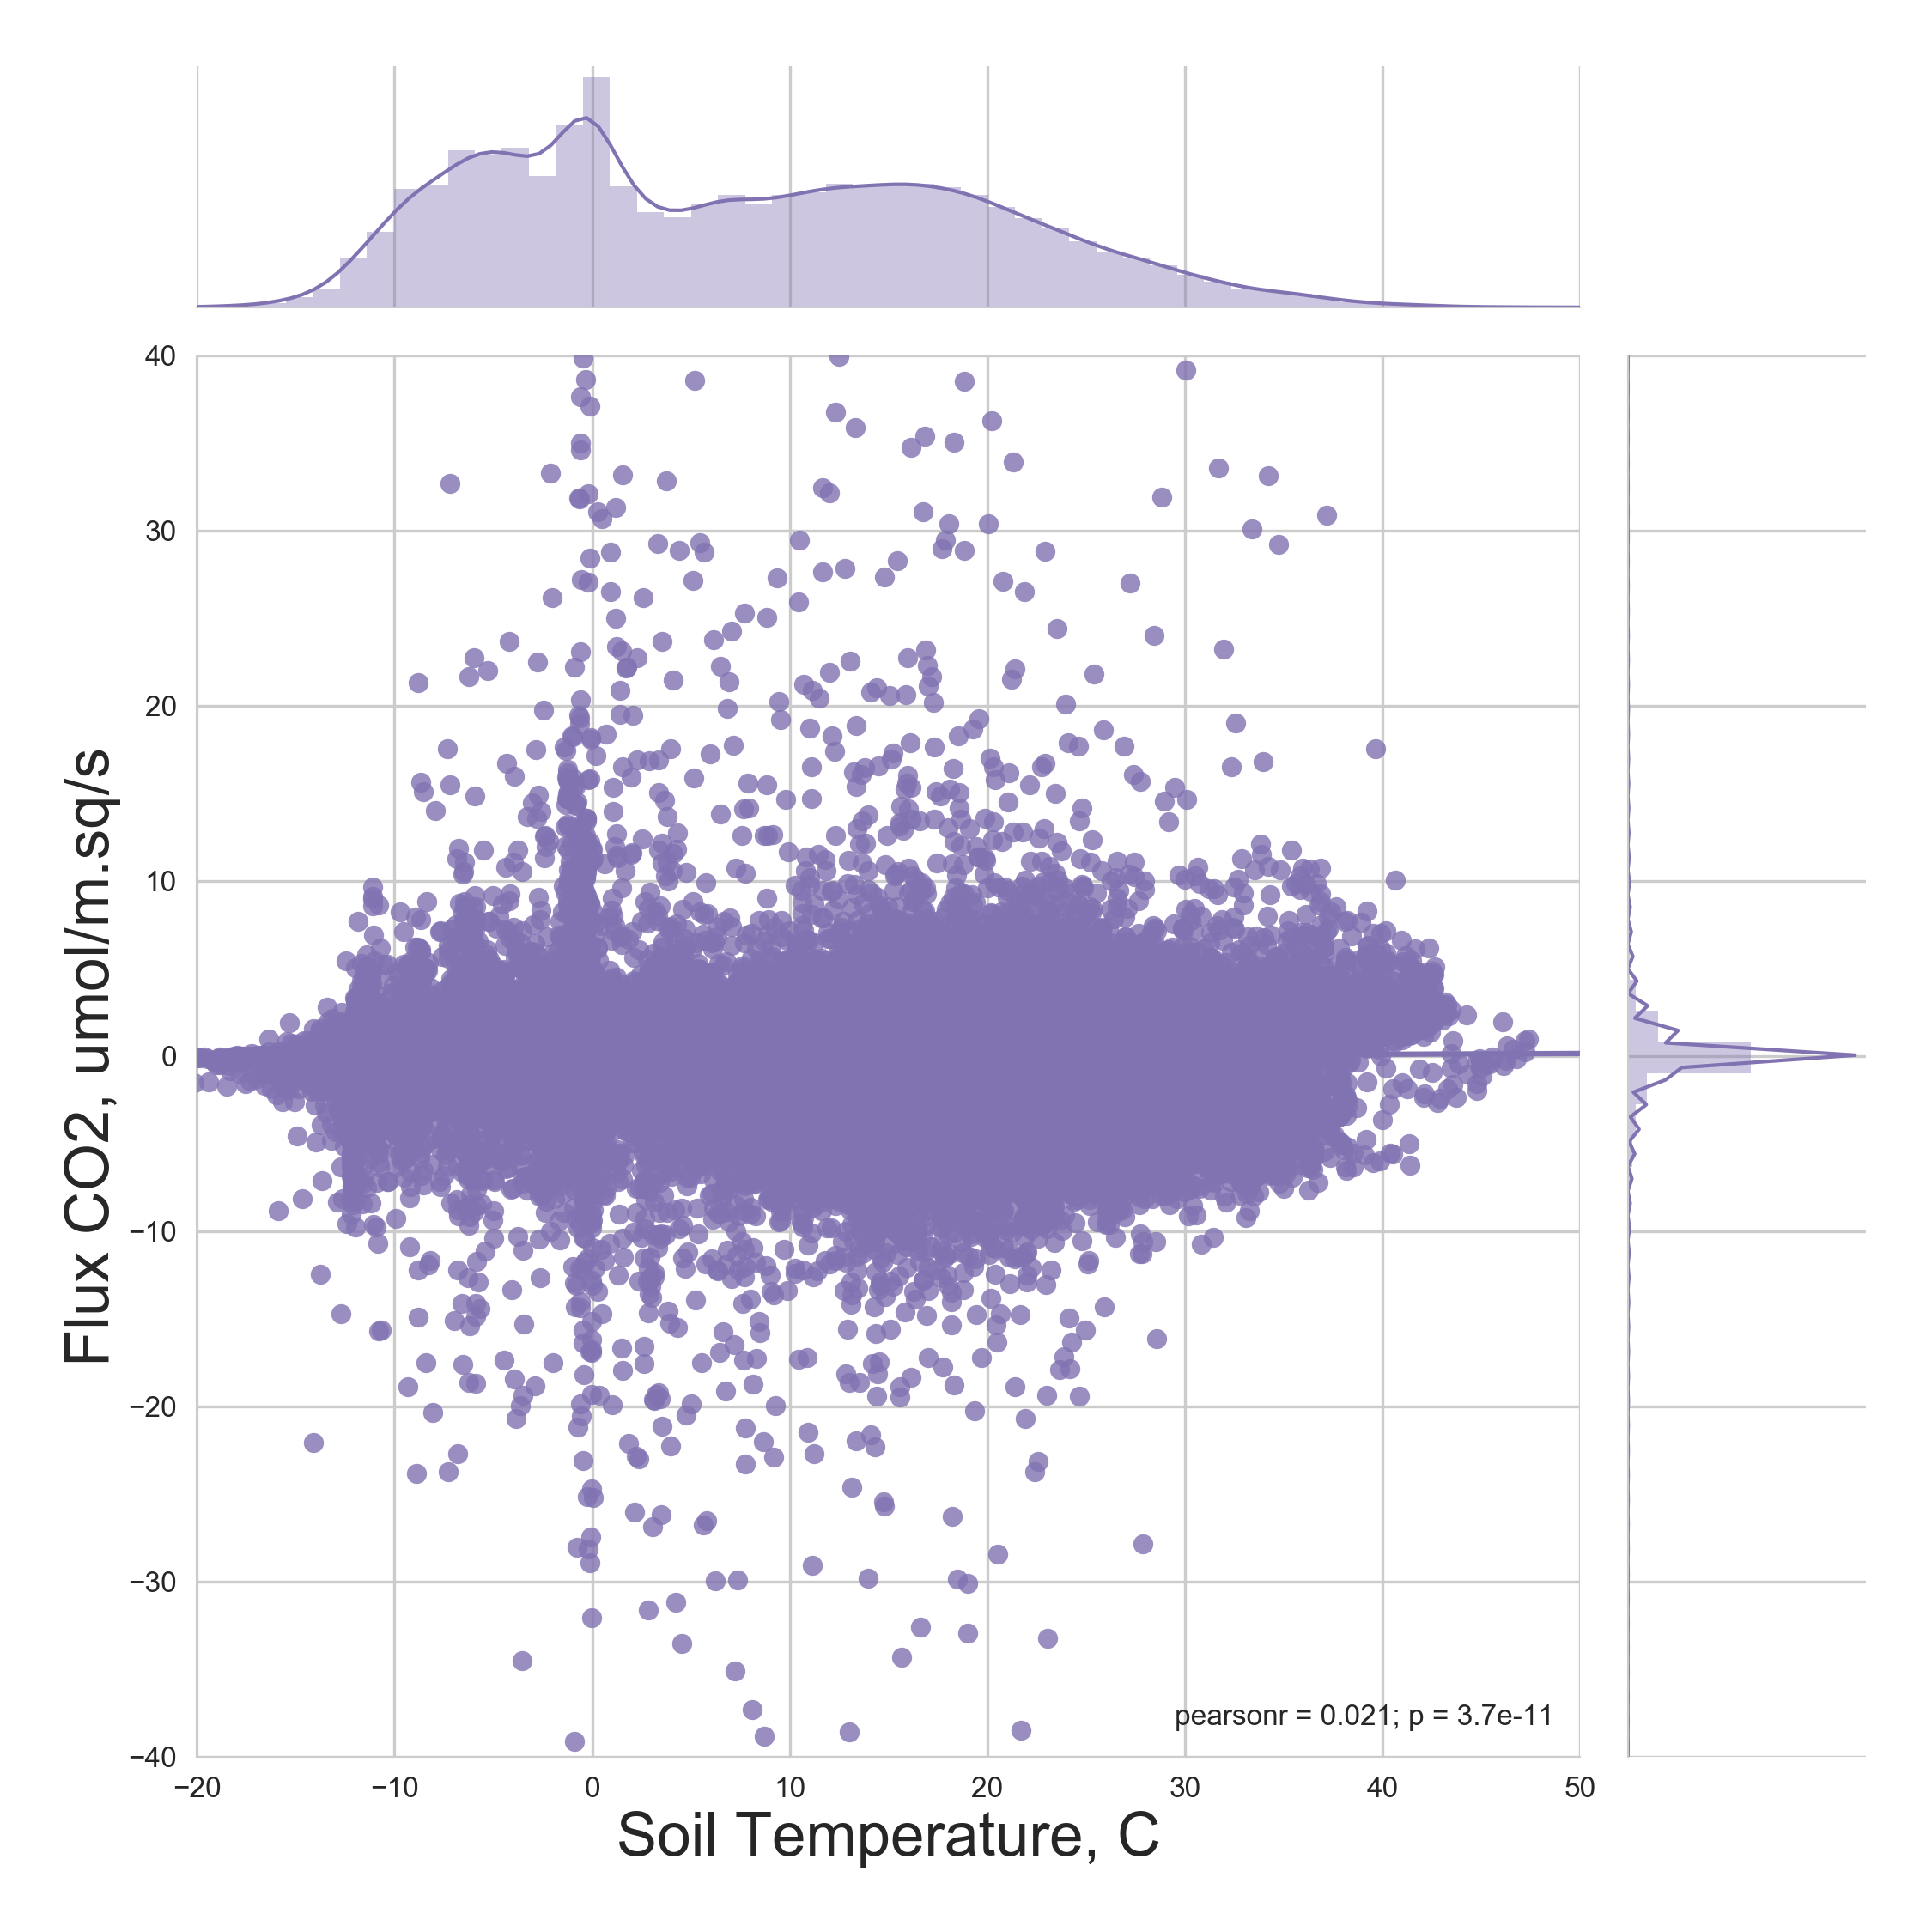
\includegraphics[width=\textwidth]{FvsT/US-FPe.png}\\
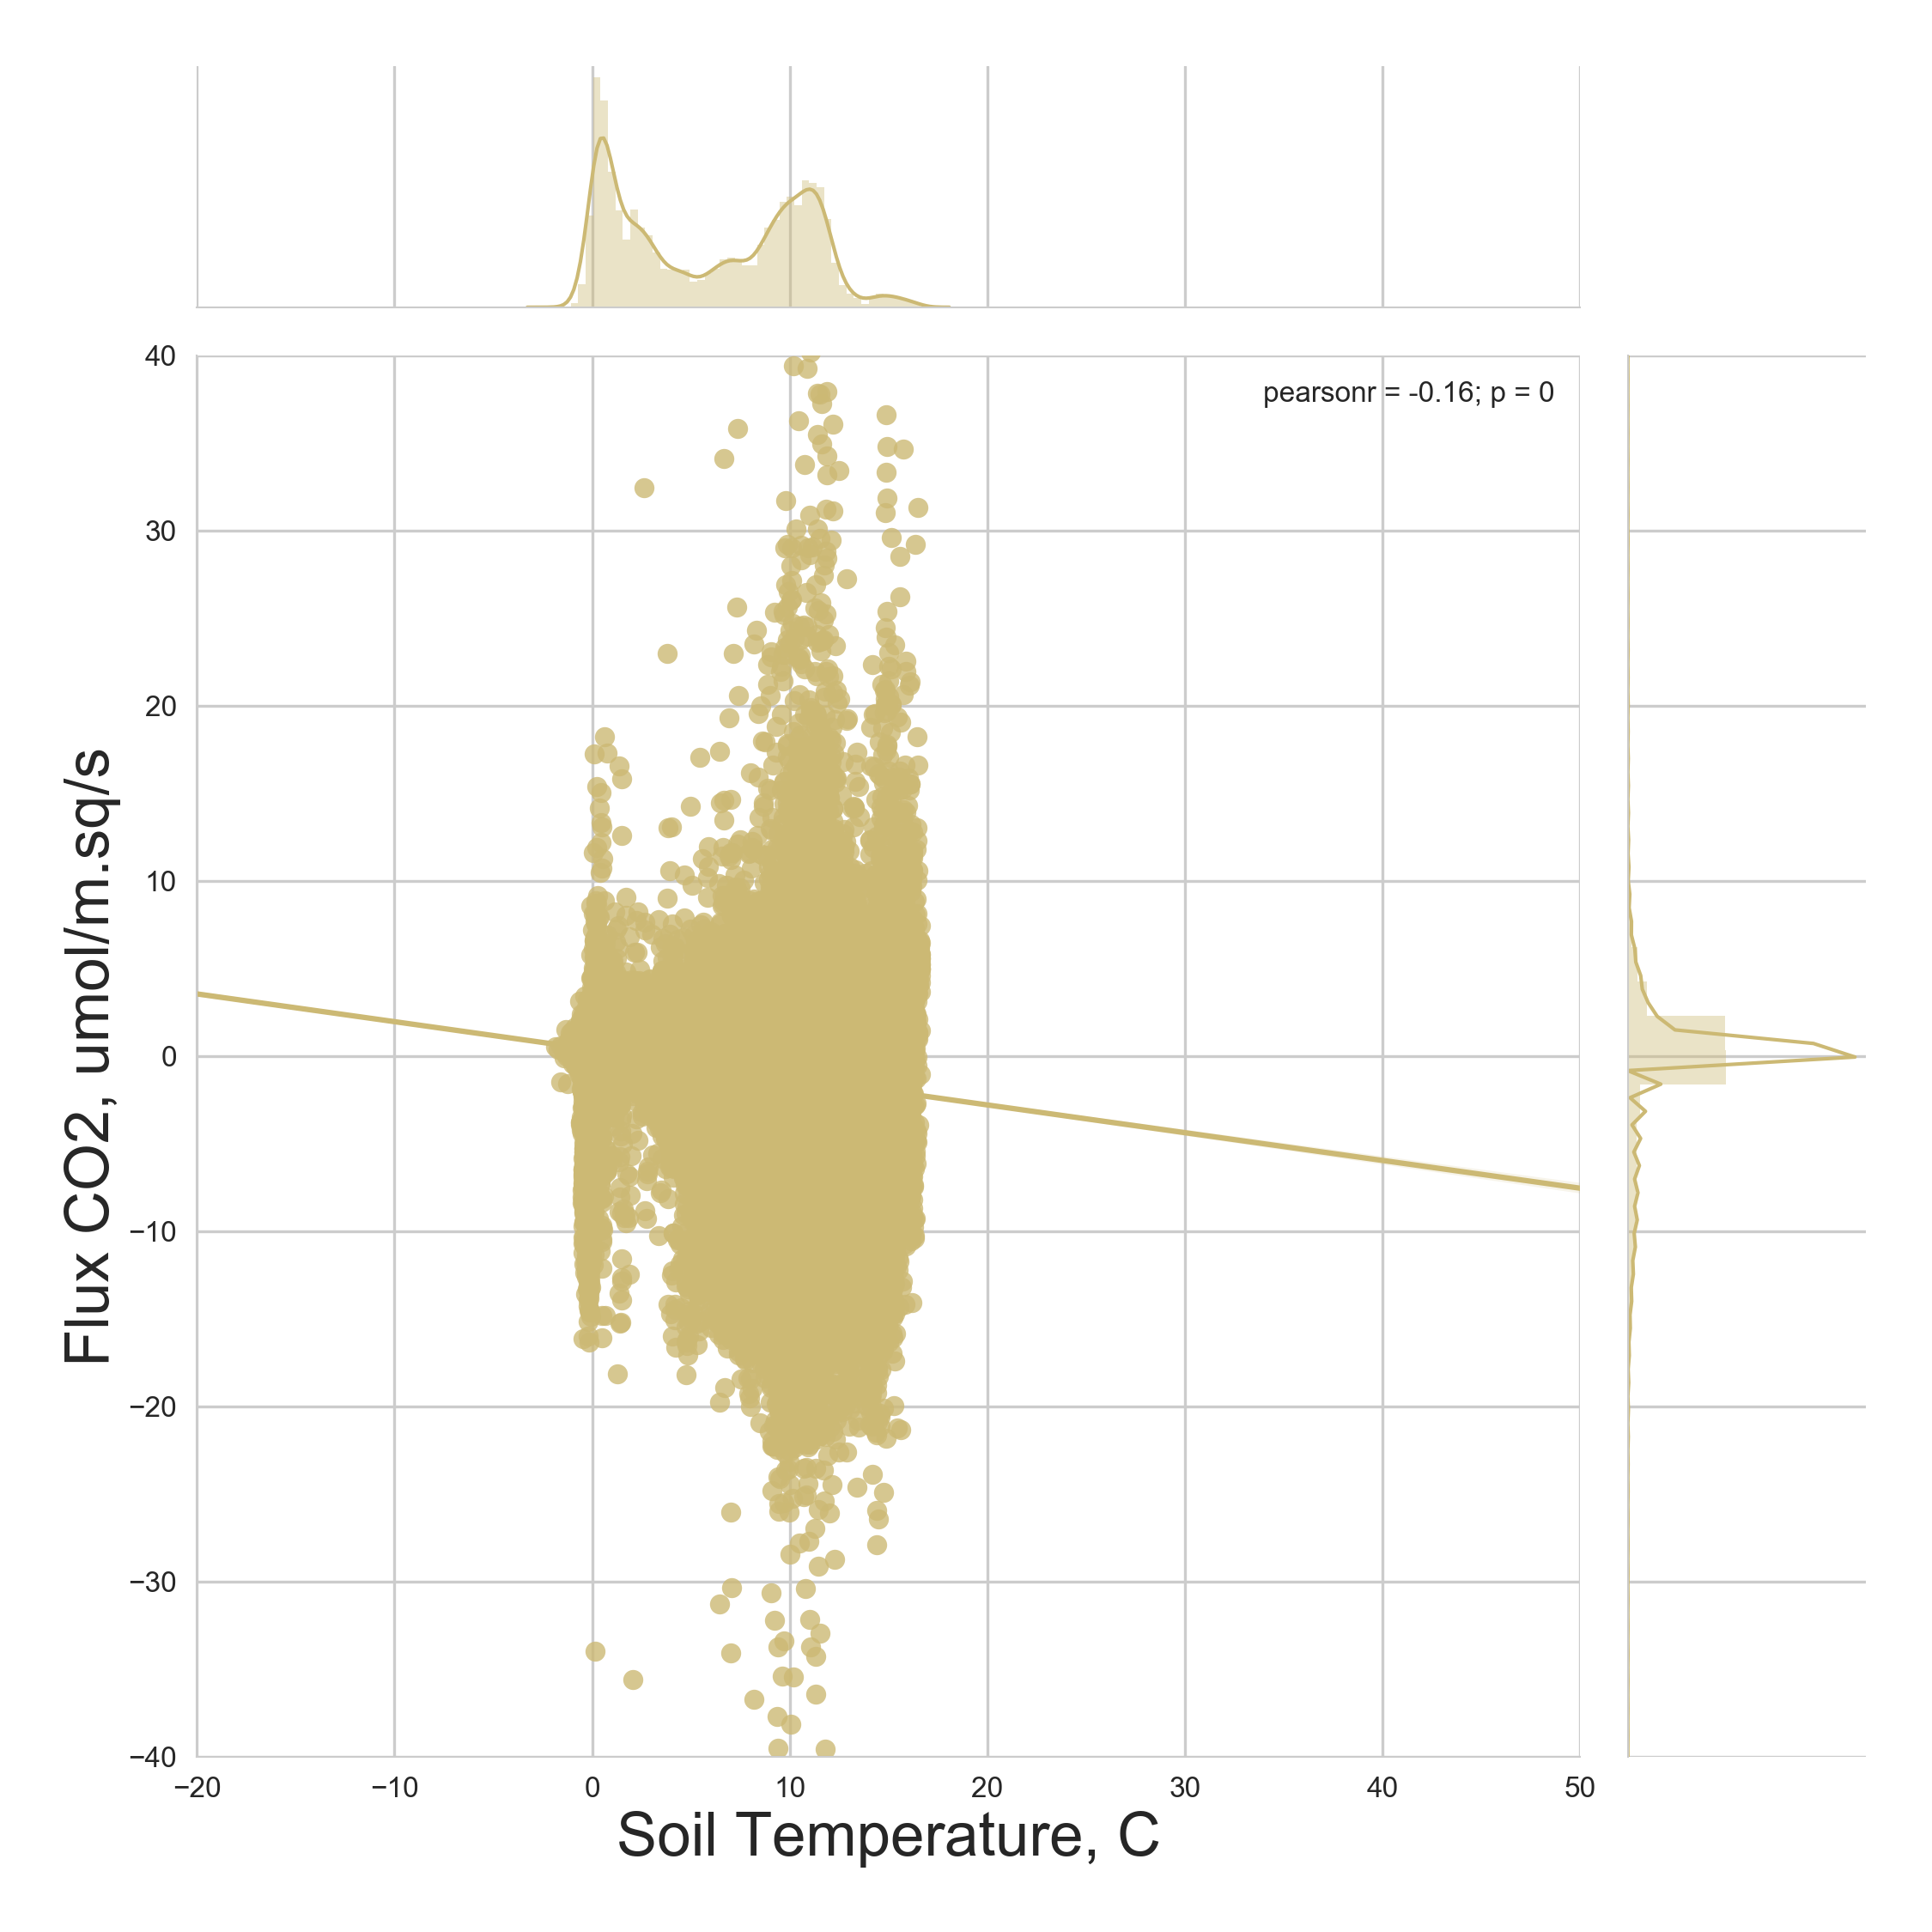
\includegraphics[width=\textwidth]{FvsT/US-Los.png}
\end{columns}

\end{frame}

\begin{frame}
\frametitle{Flux vs Precipitation}

\begin{columns}[t]
\column{.35\textwidth}
\centering
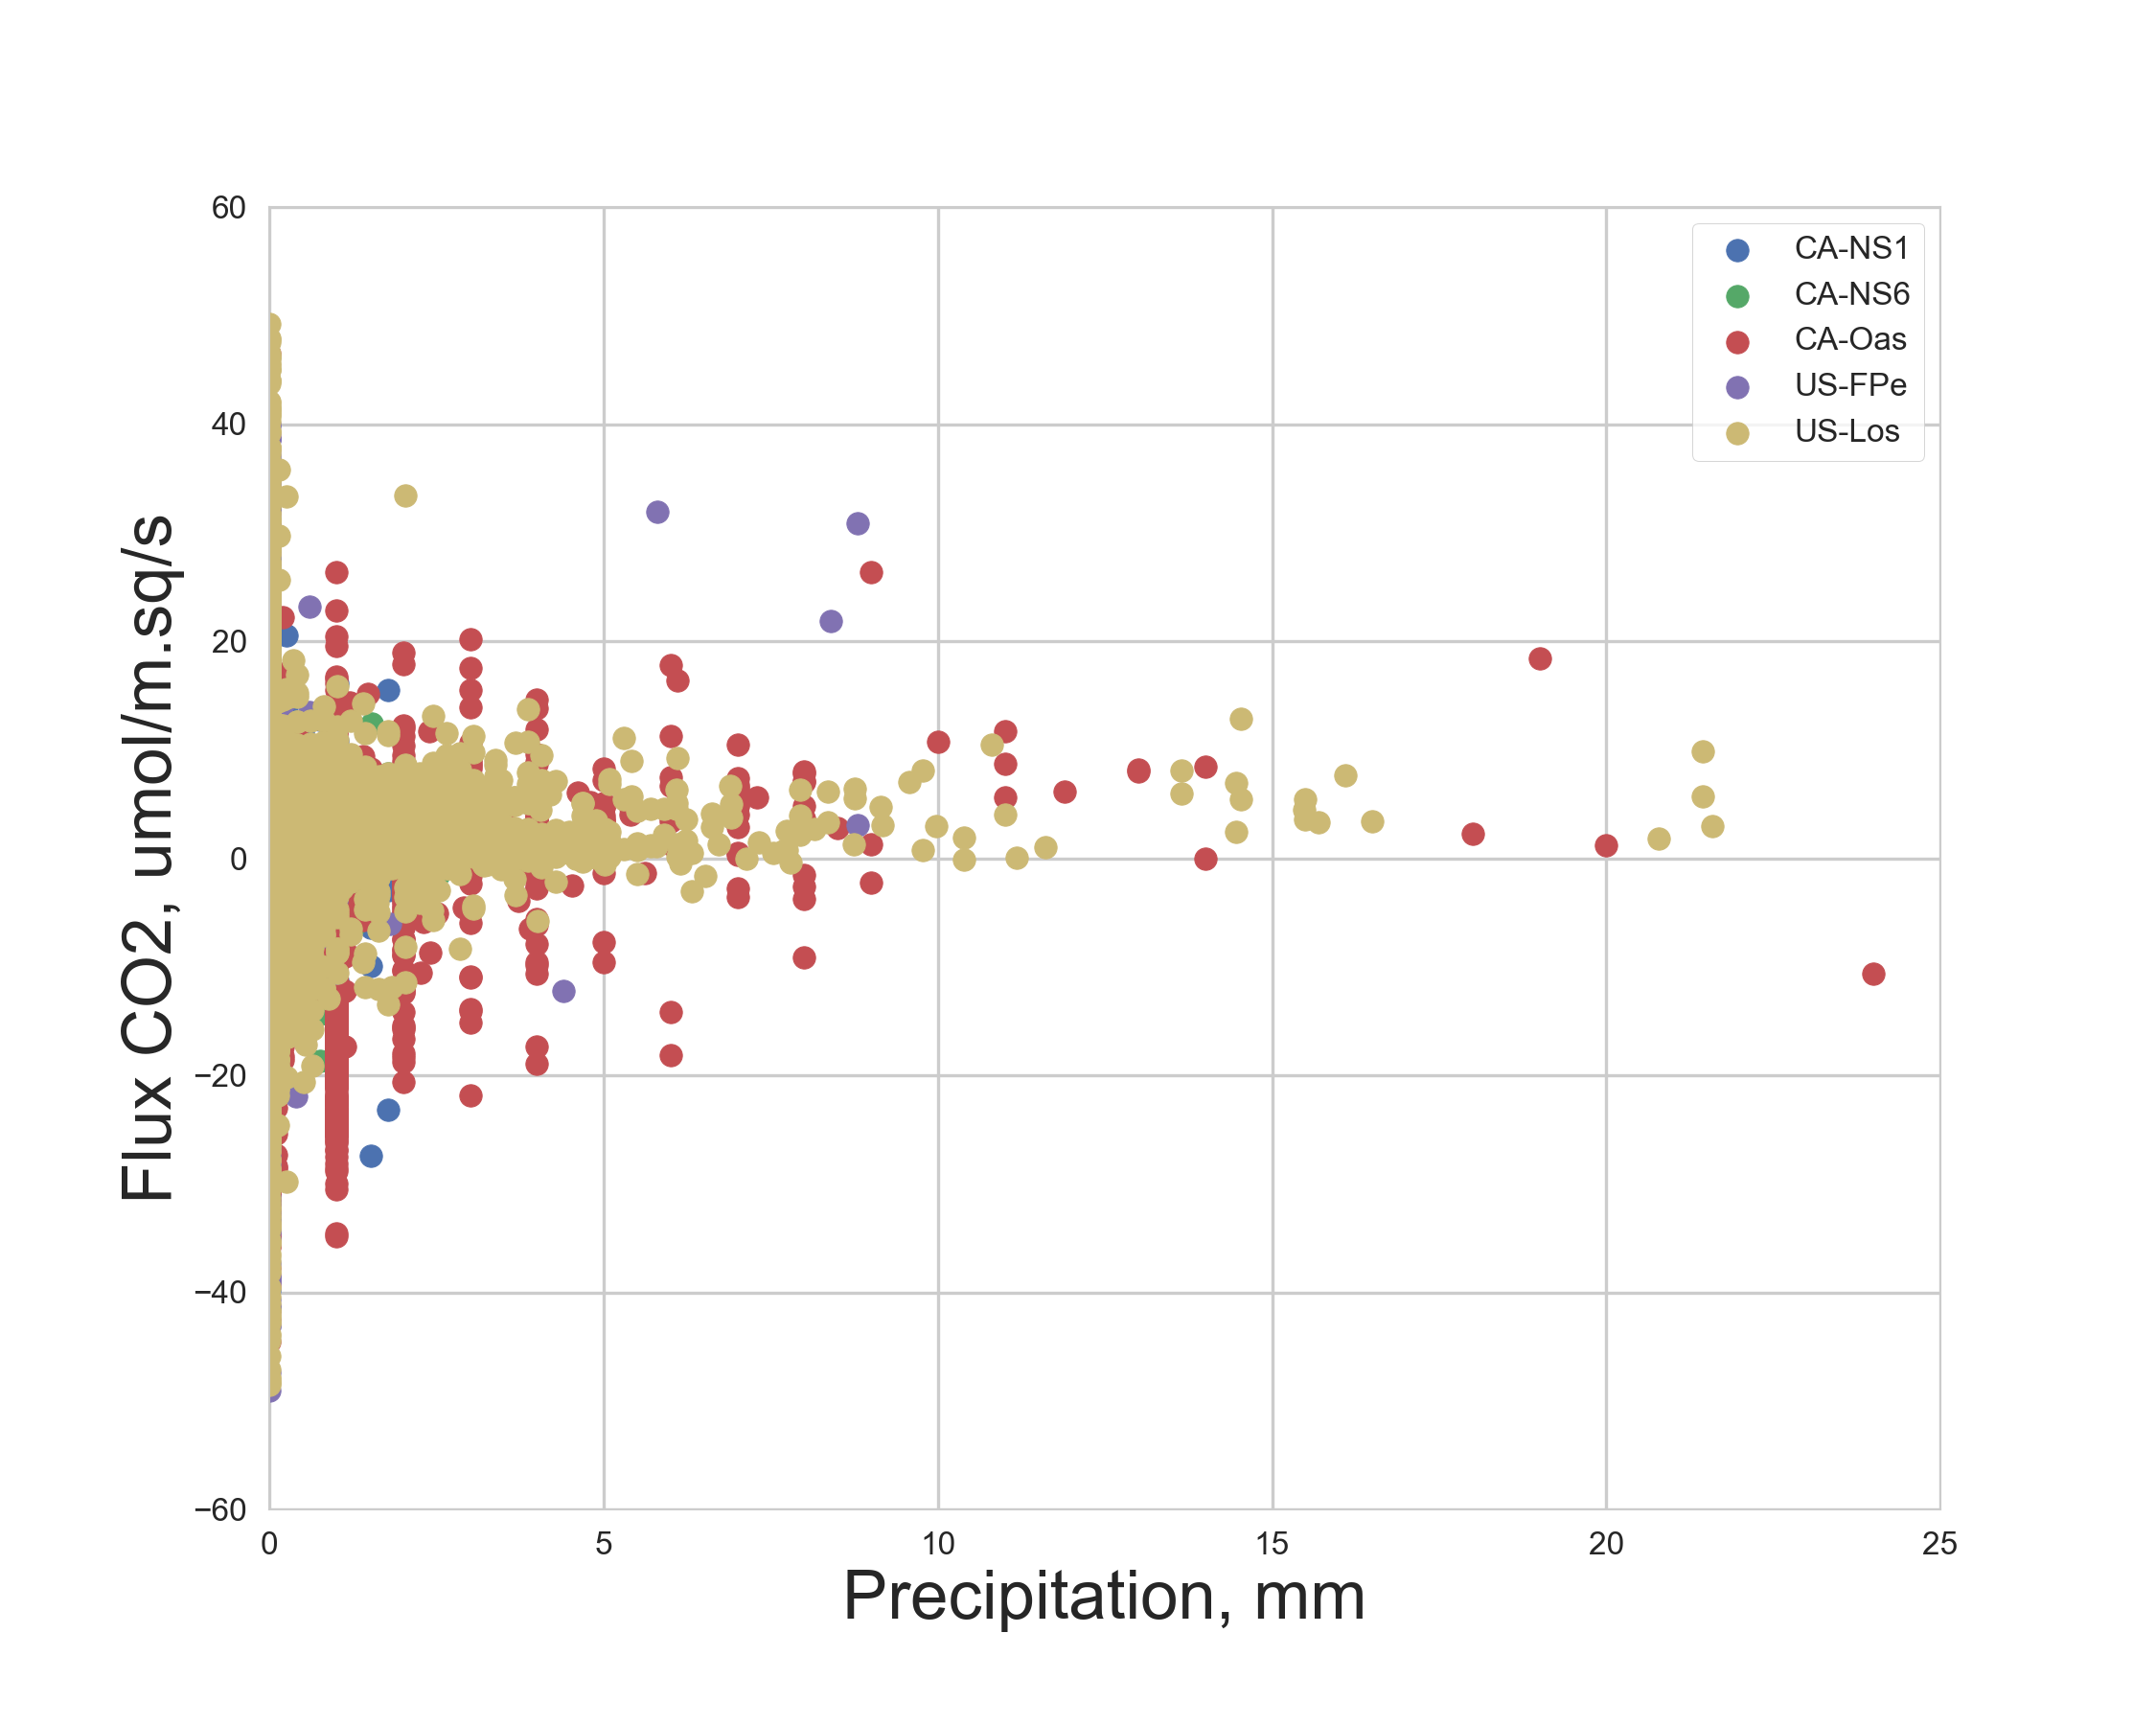
\includegraphics[width=\textwidth]{FvsP/all.png}\\
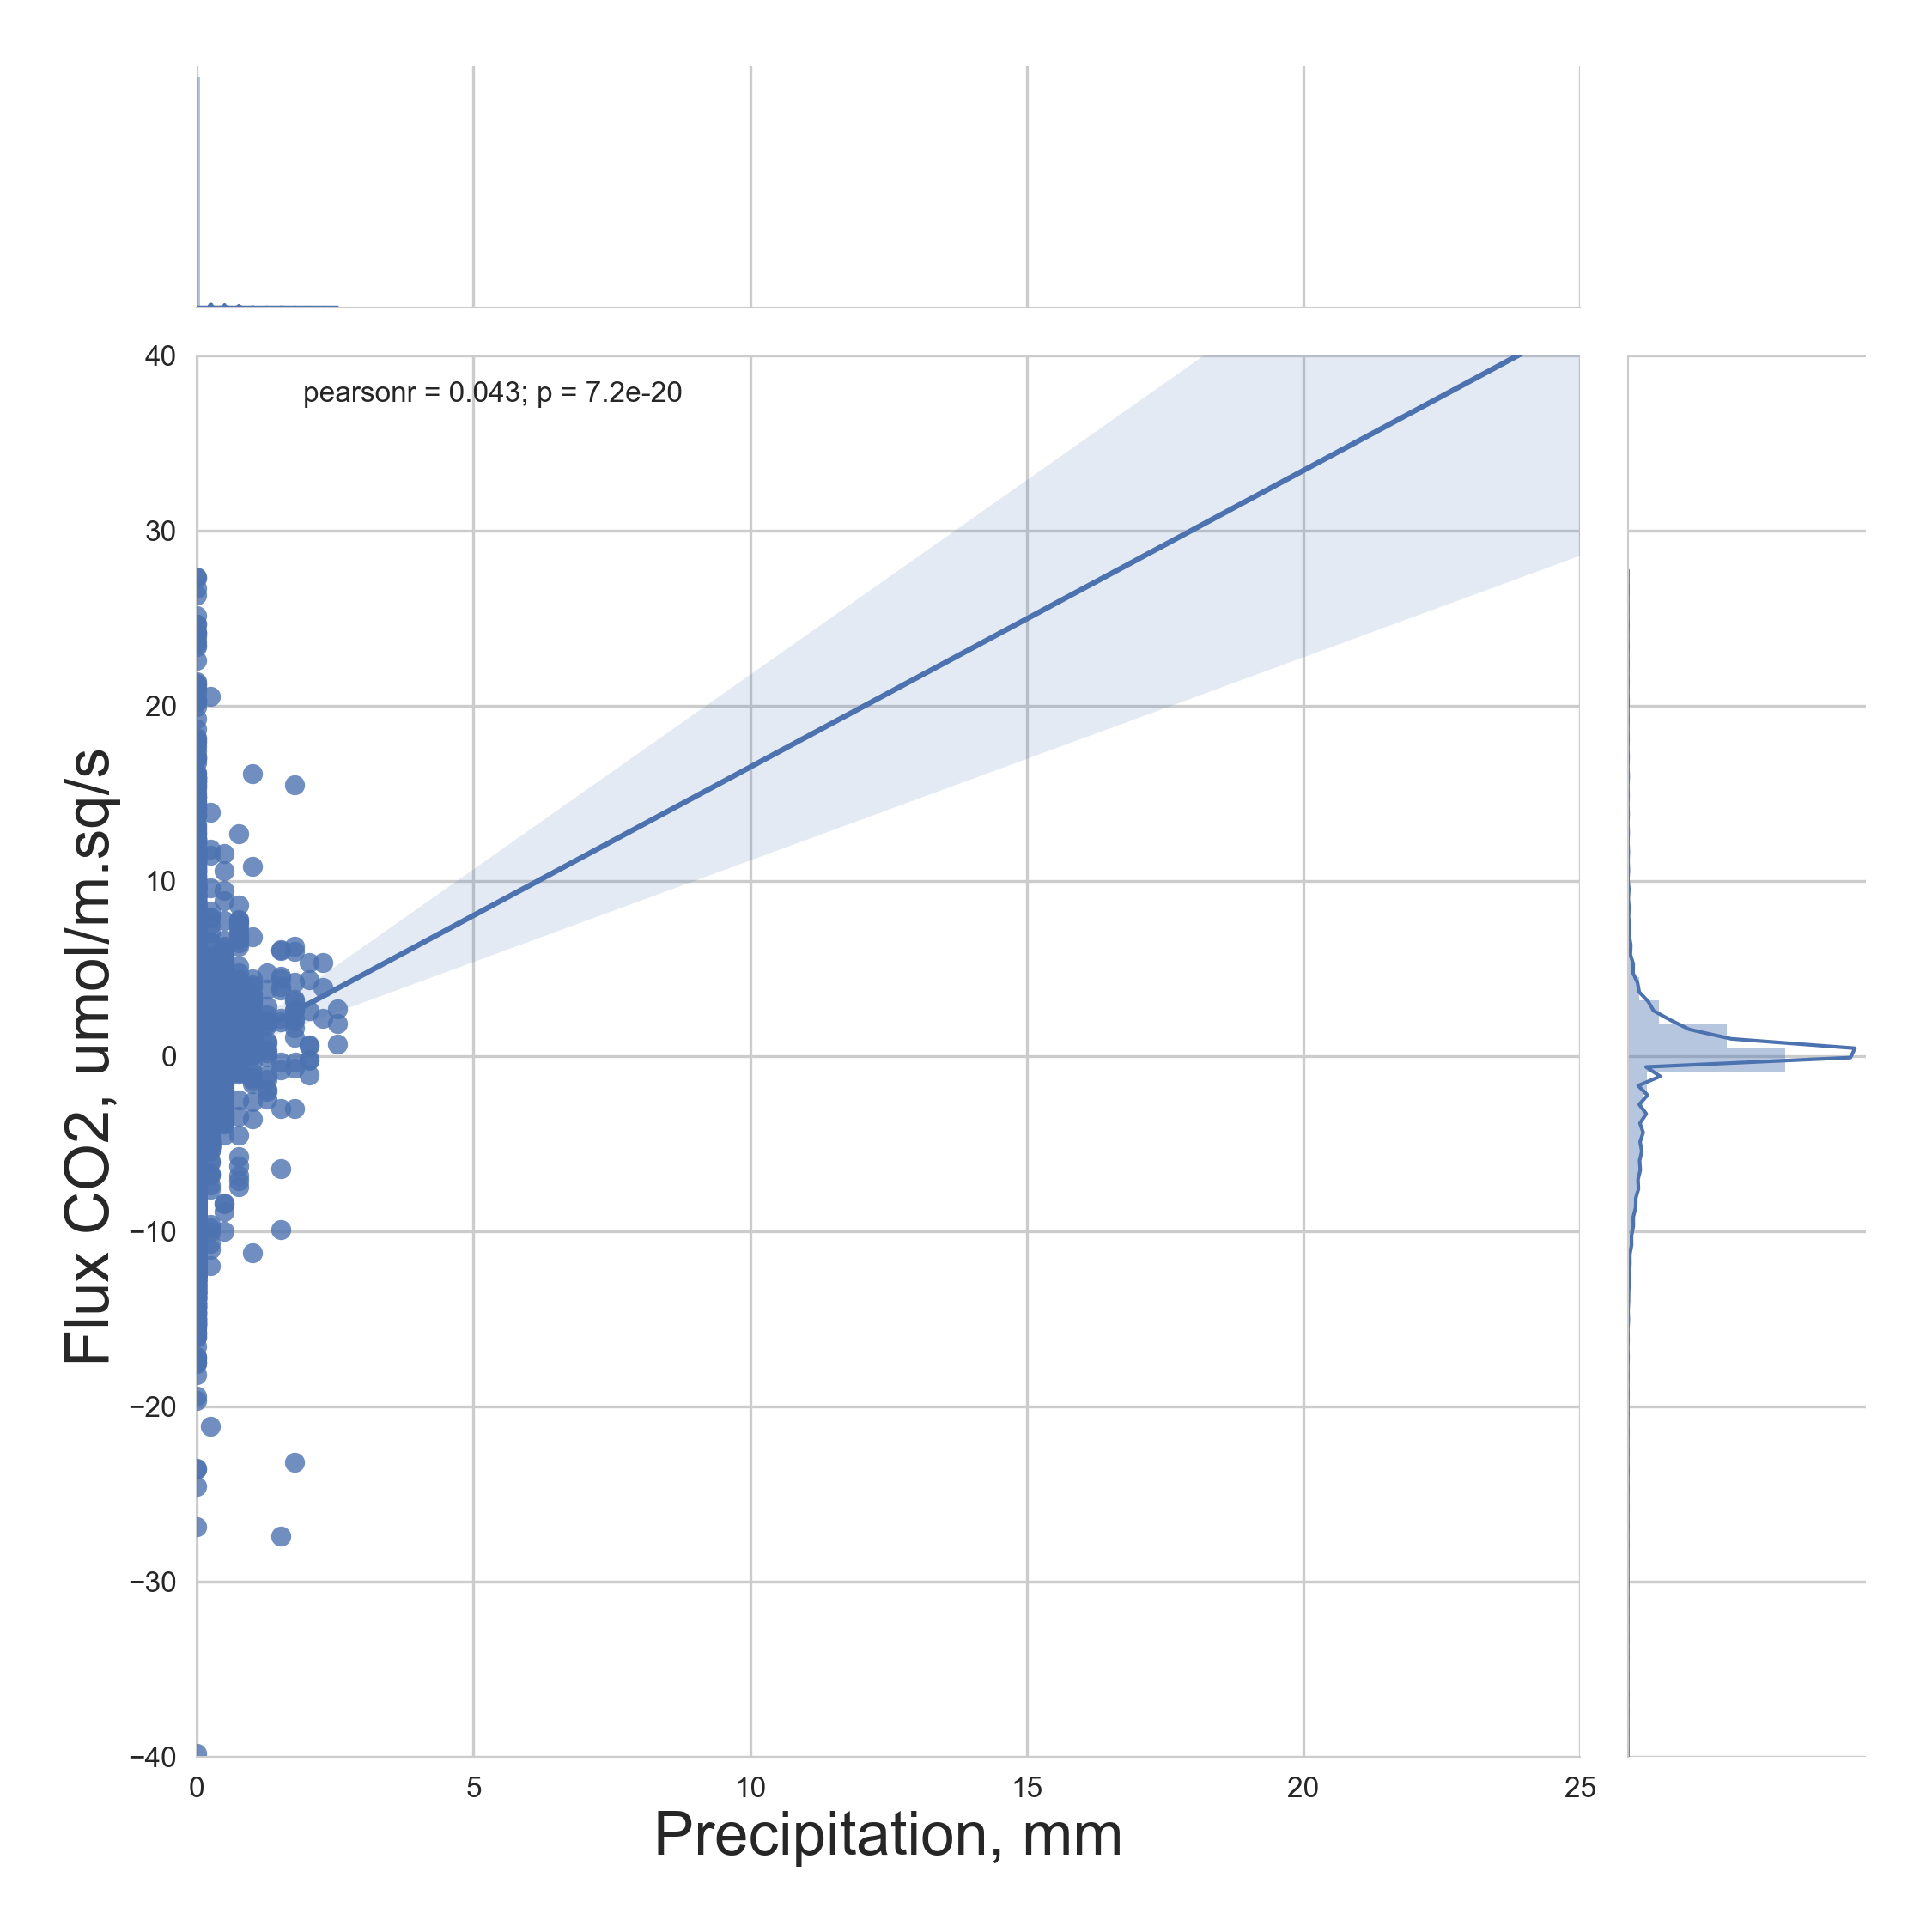
\includegraphics[width=\textwidth]{FvsP/CA-NS1.png}
\column{.35\textwidth}
\centering
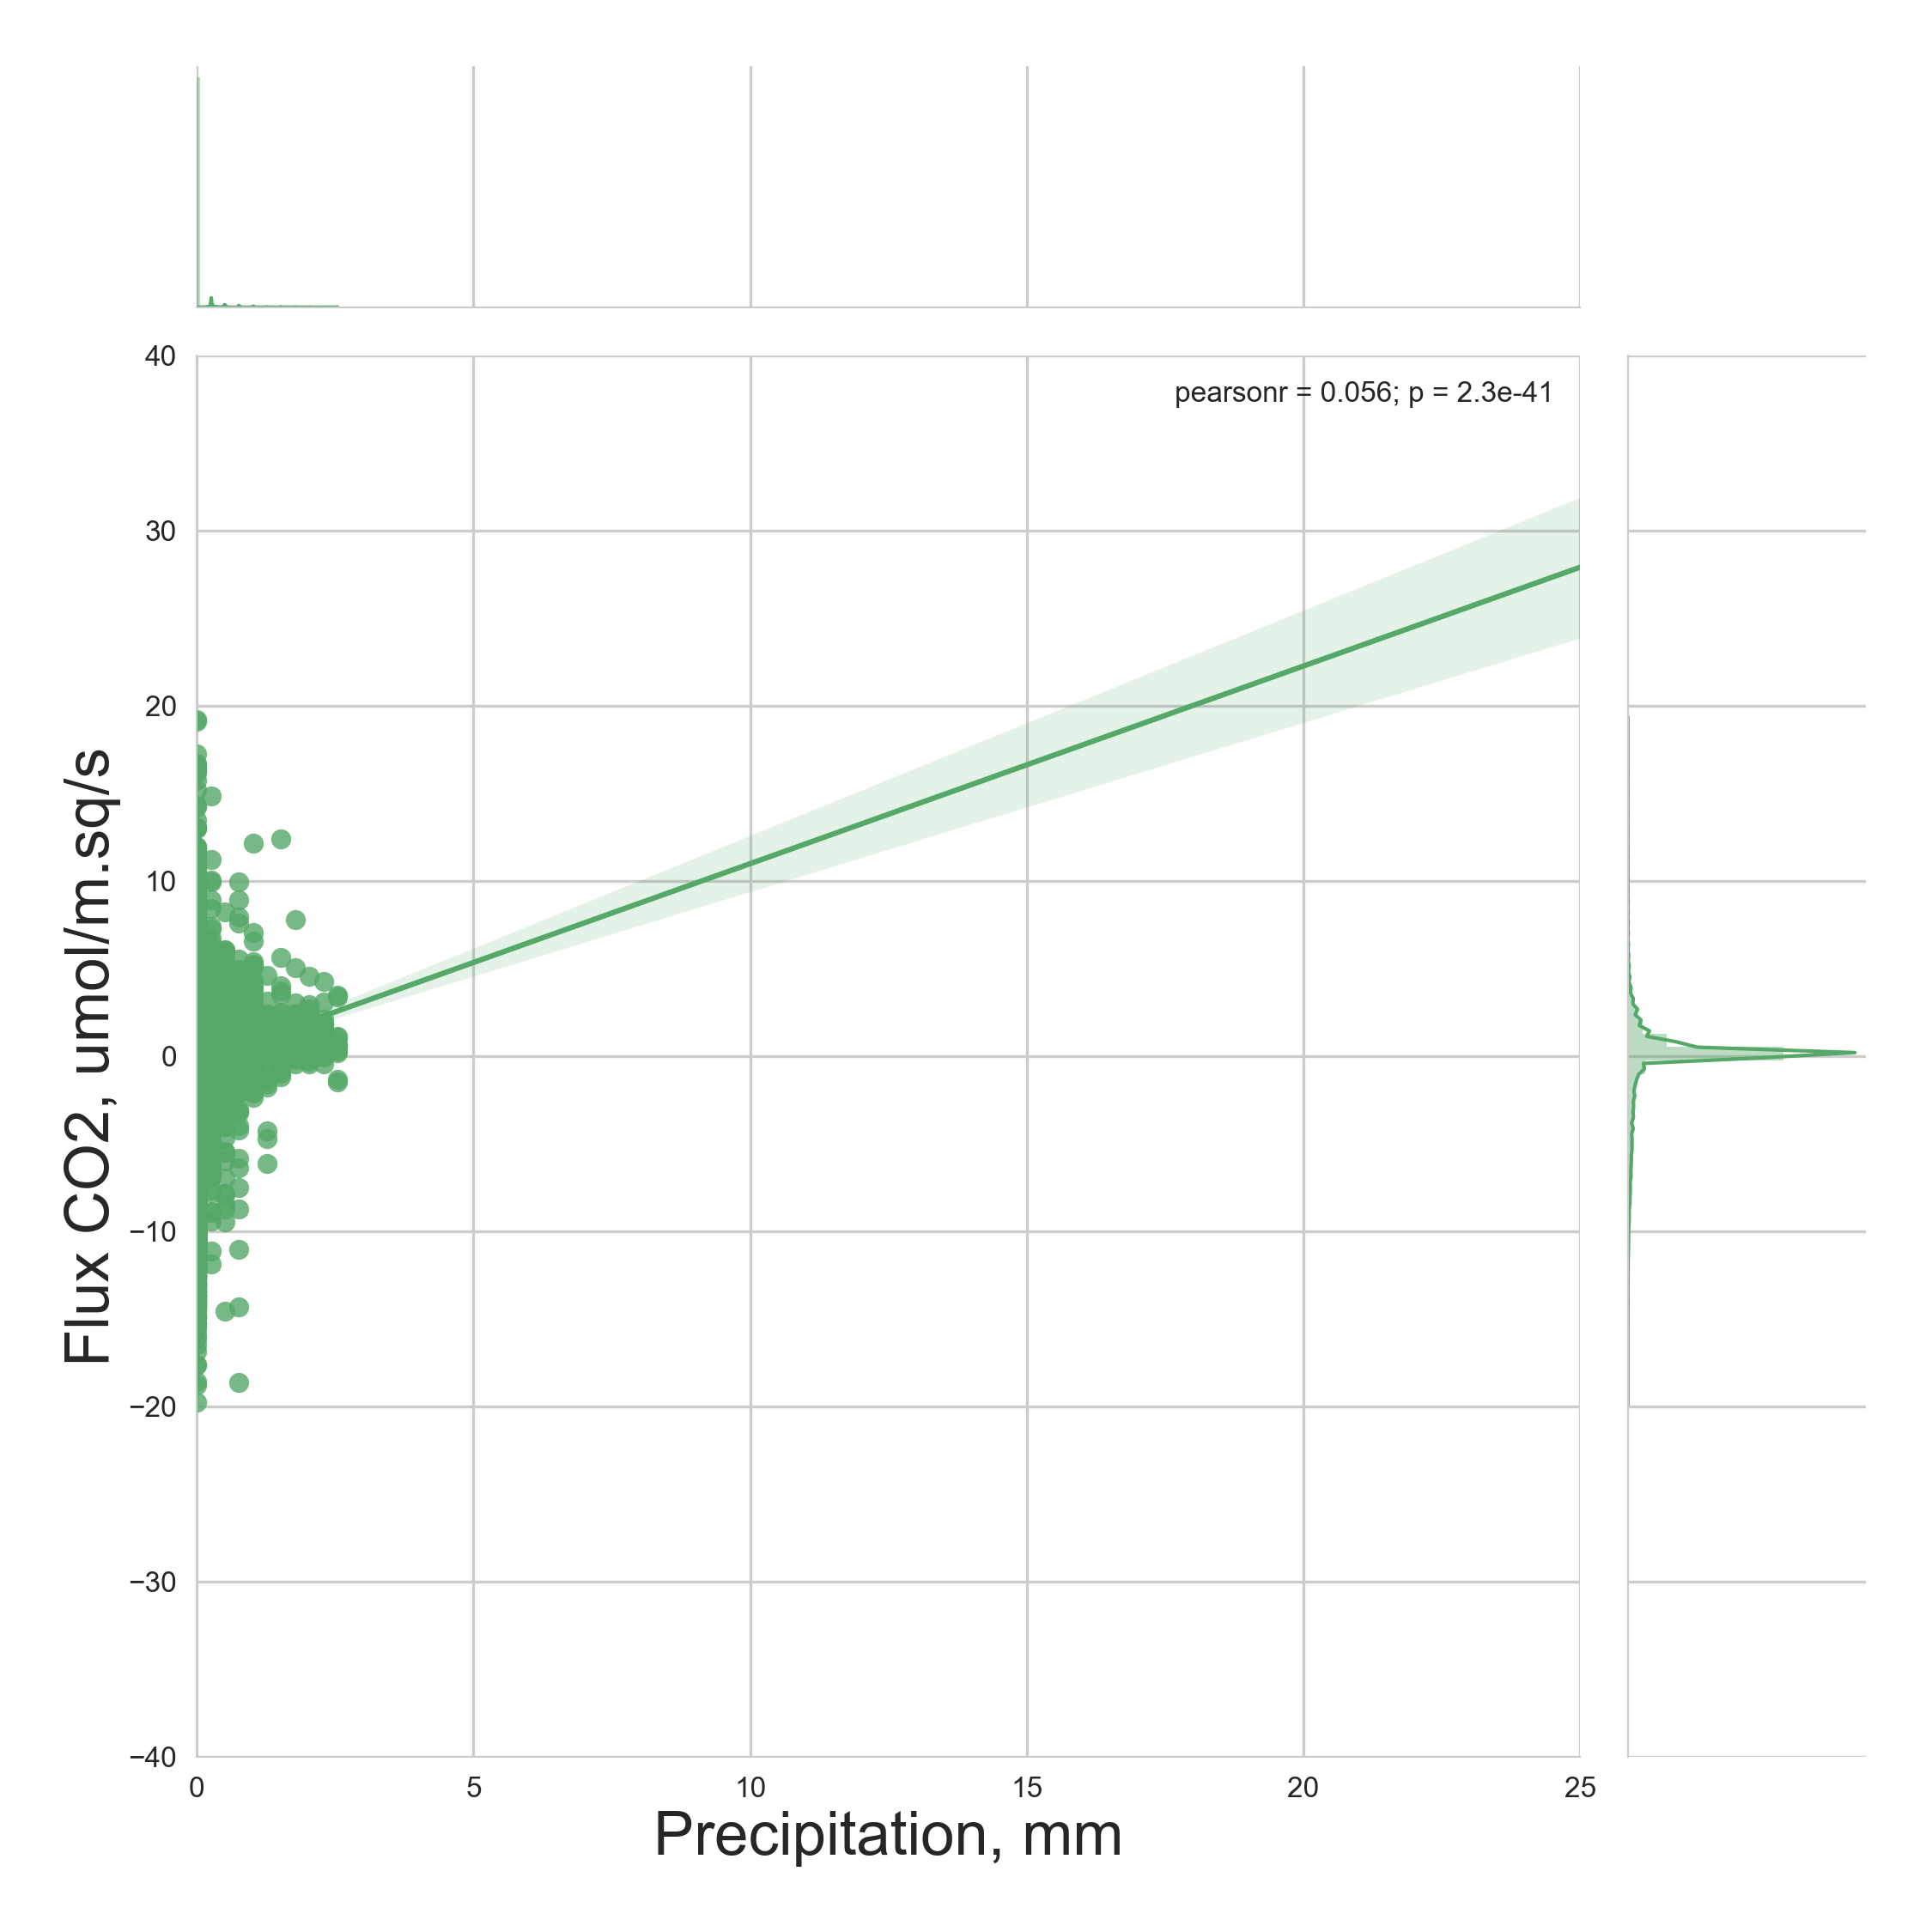
\includegraphics[width=\textwidth]{FvsP/CA-NS6.png}\\
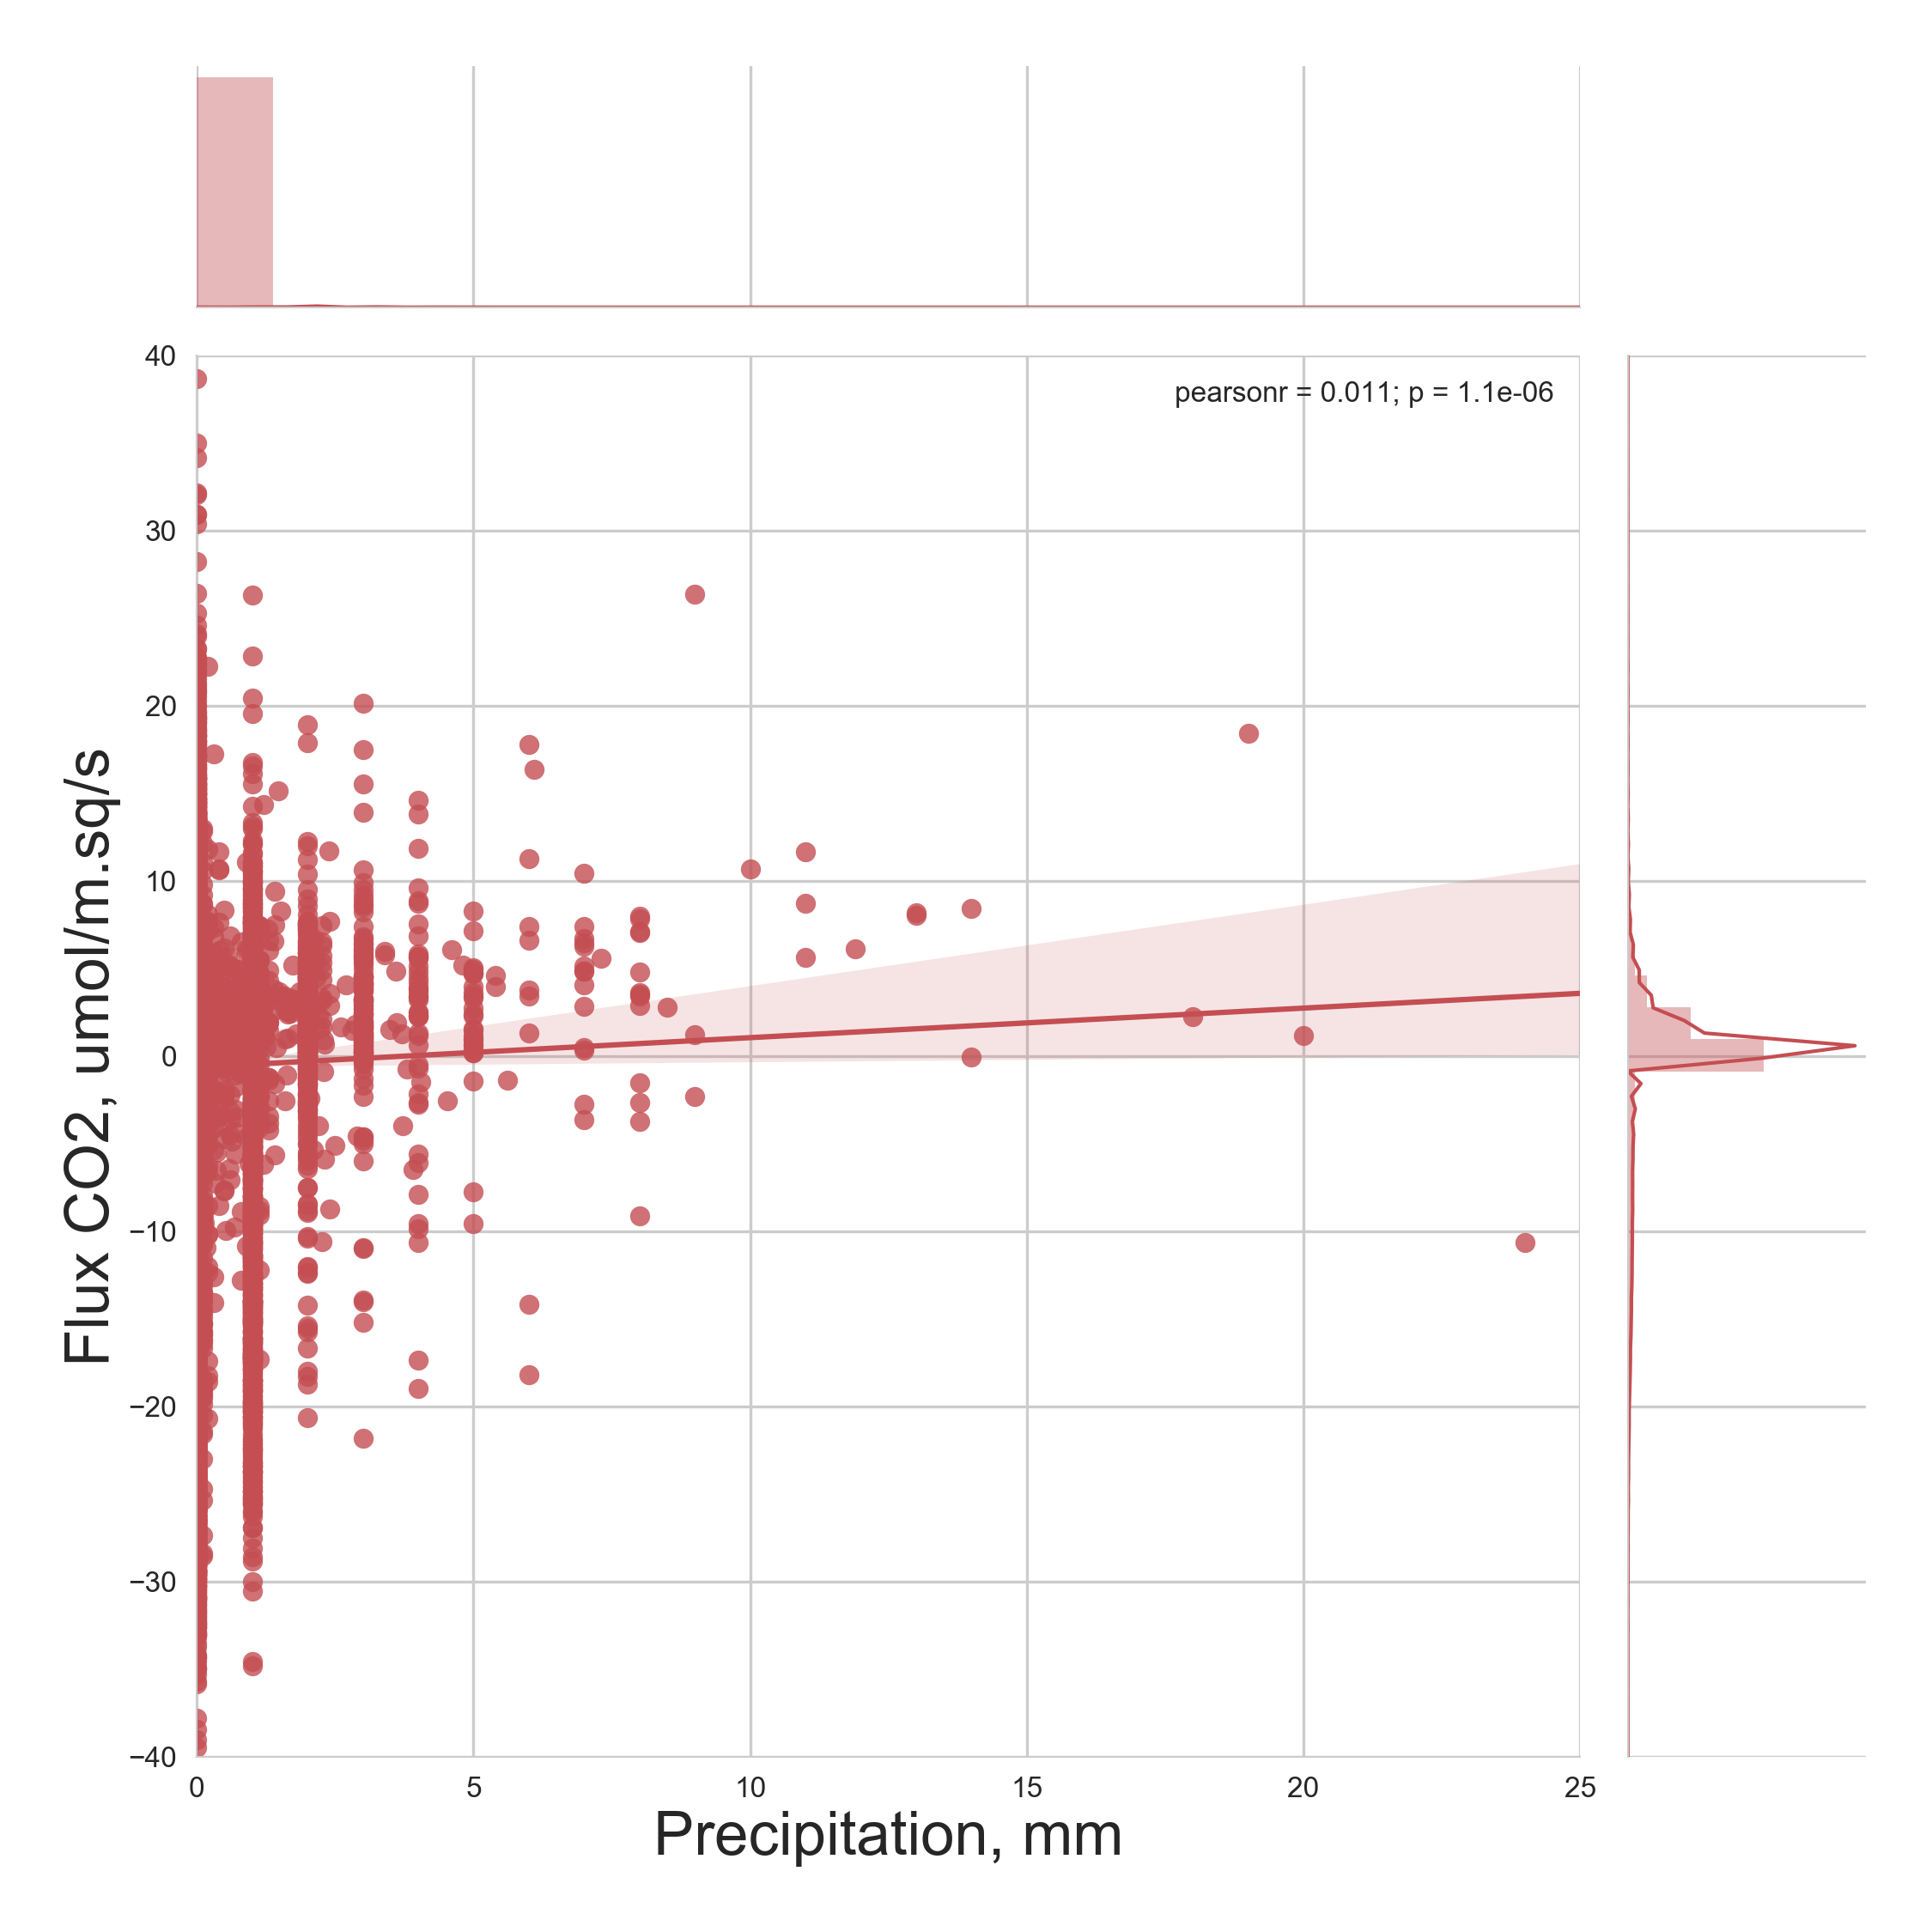
\includegraphics[width=\textwidth]{FvsP/CA-Oas.png}
\column{.35\textwidth}
\centering
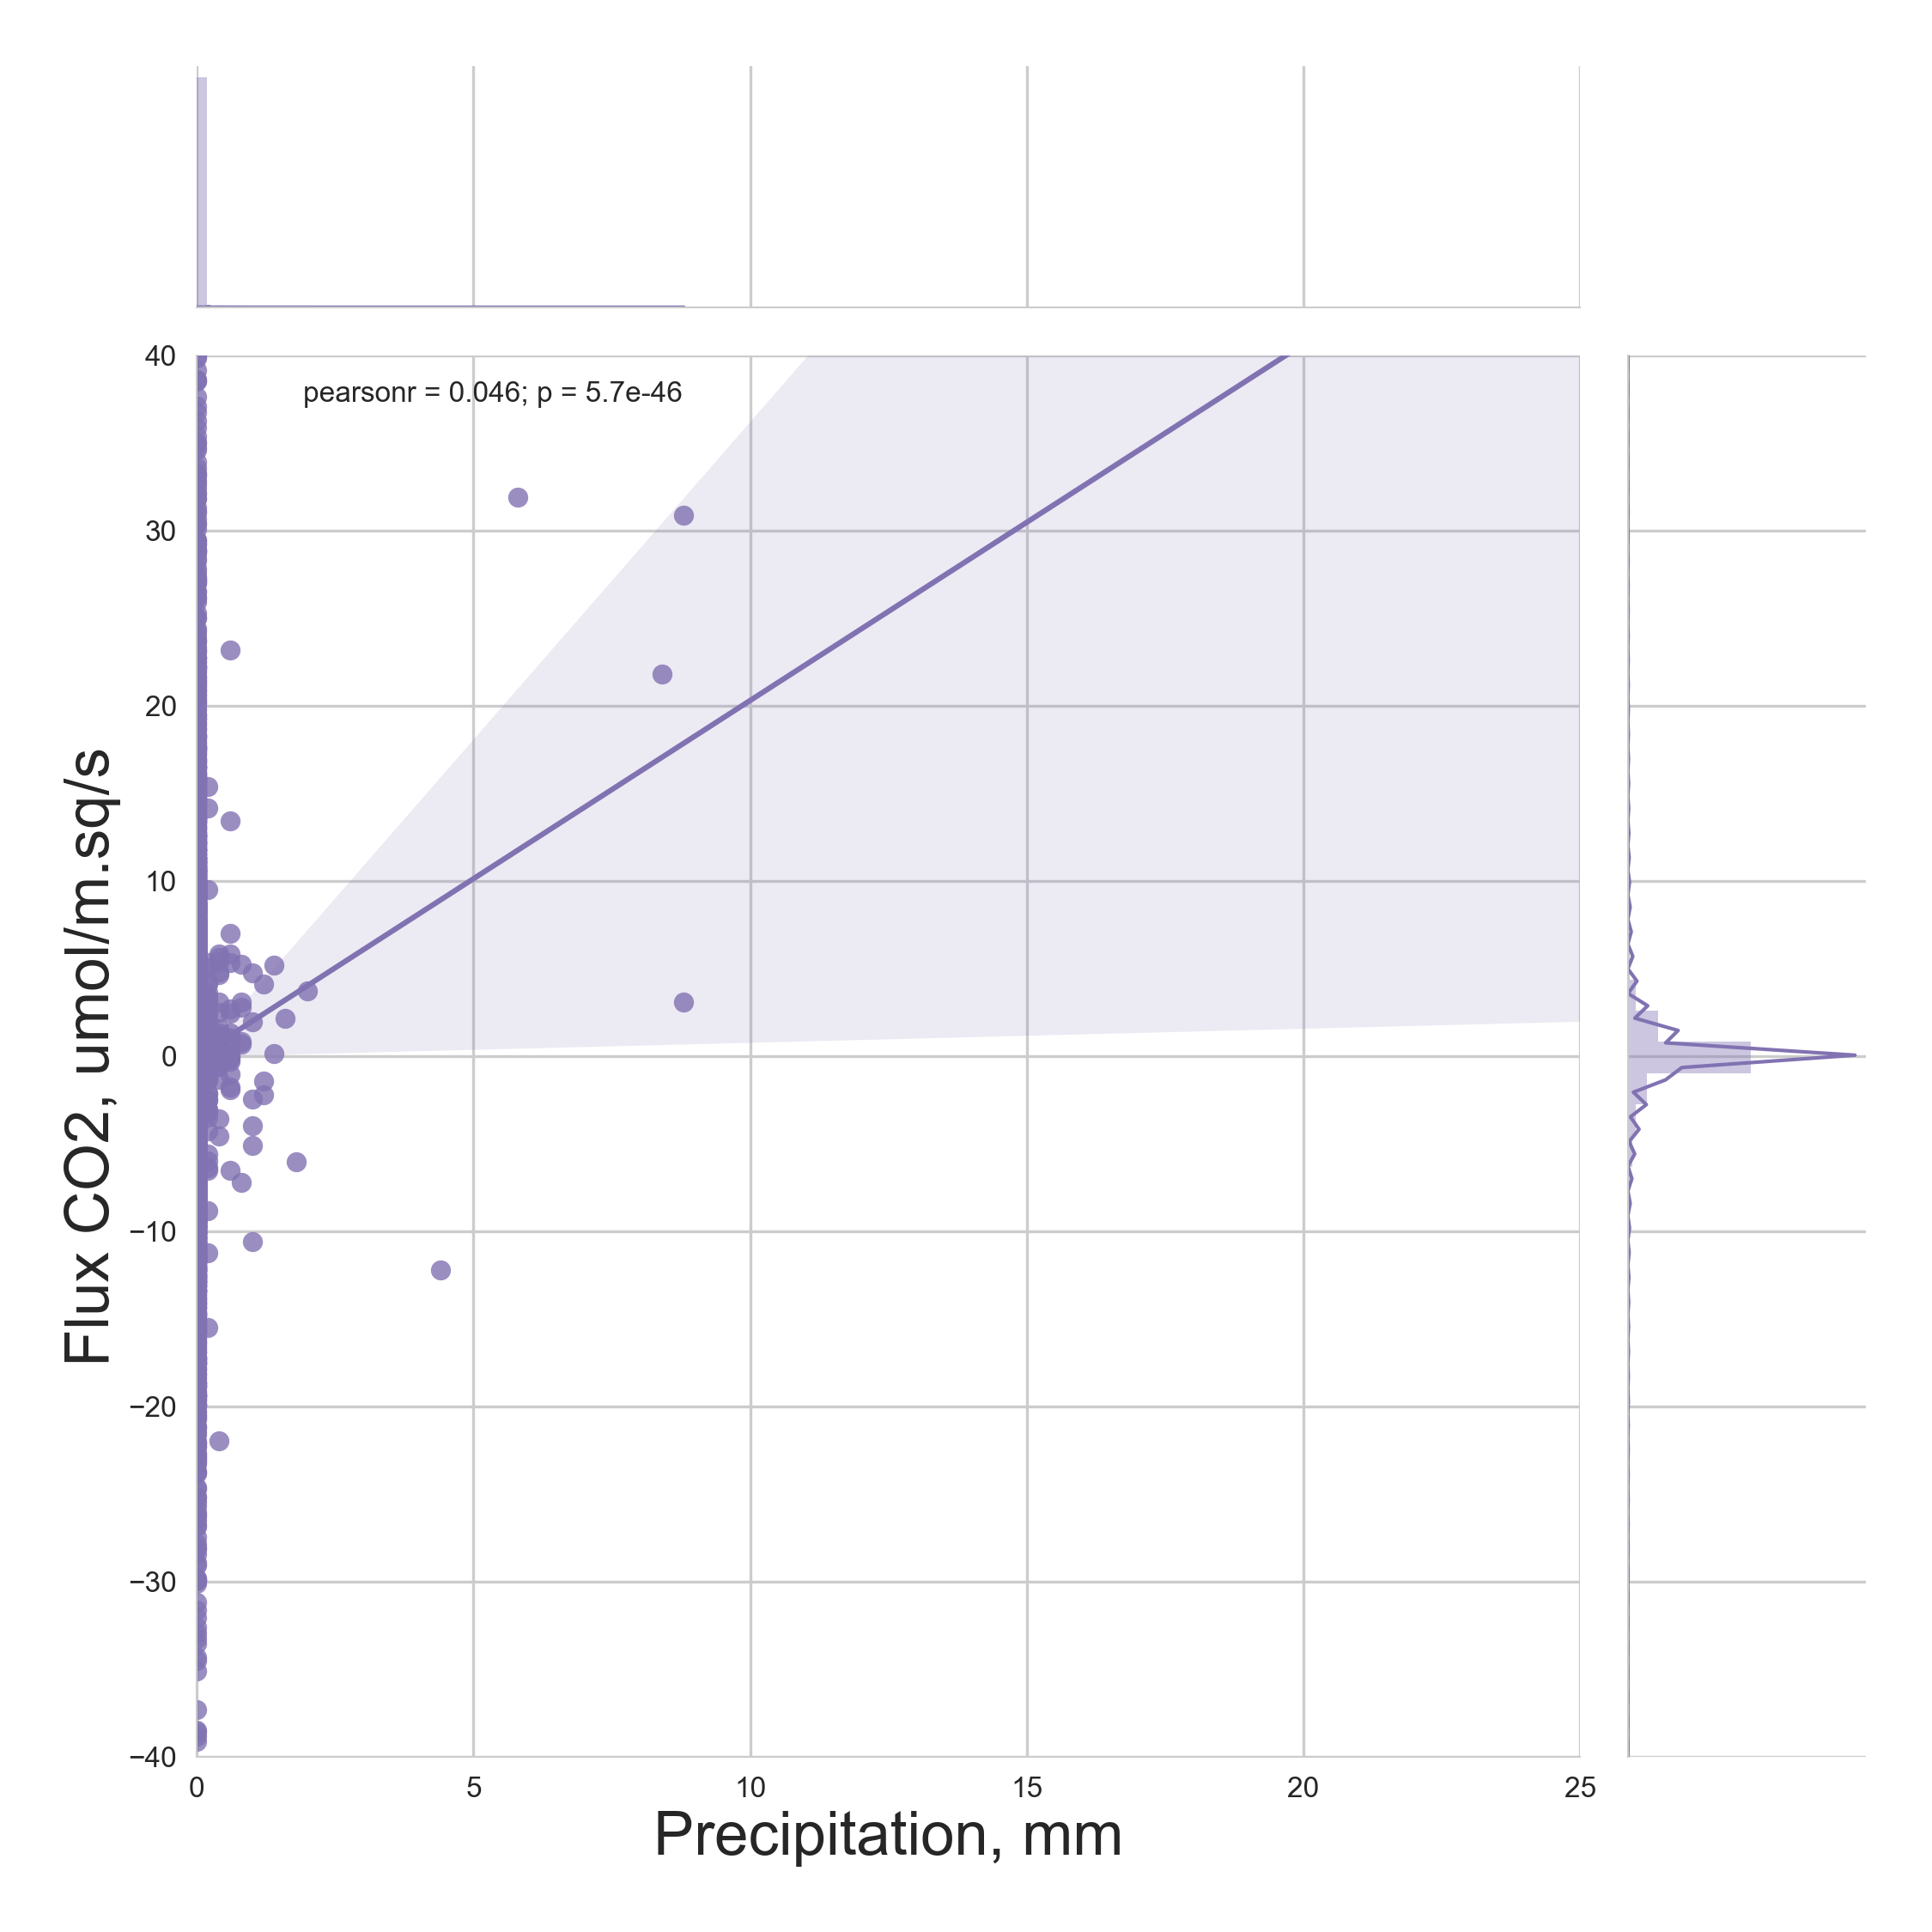
\includegraphics[width=\textwidth]{FvsP/US-FPe.png}\\
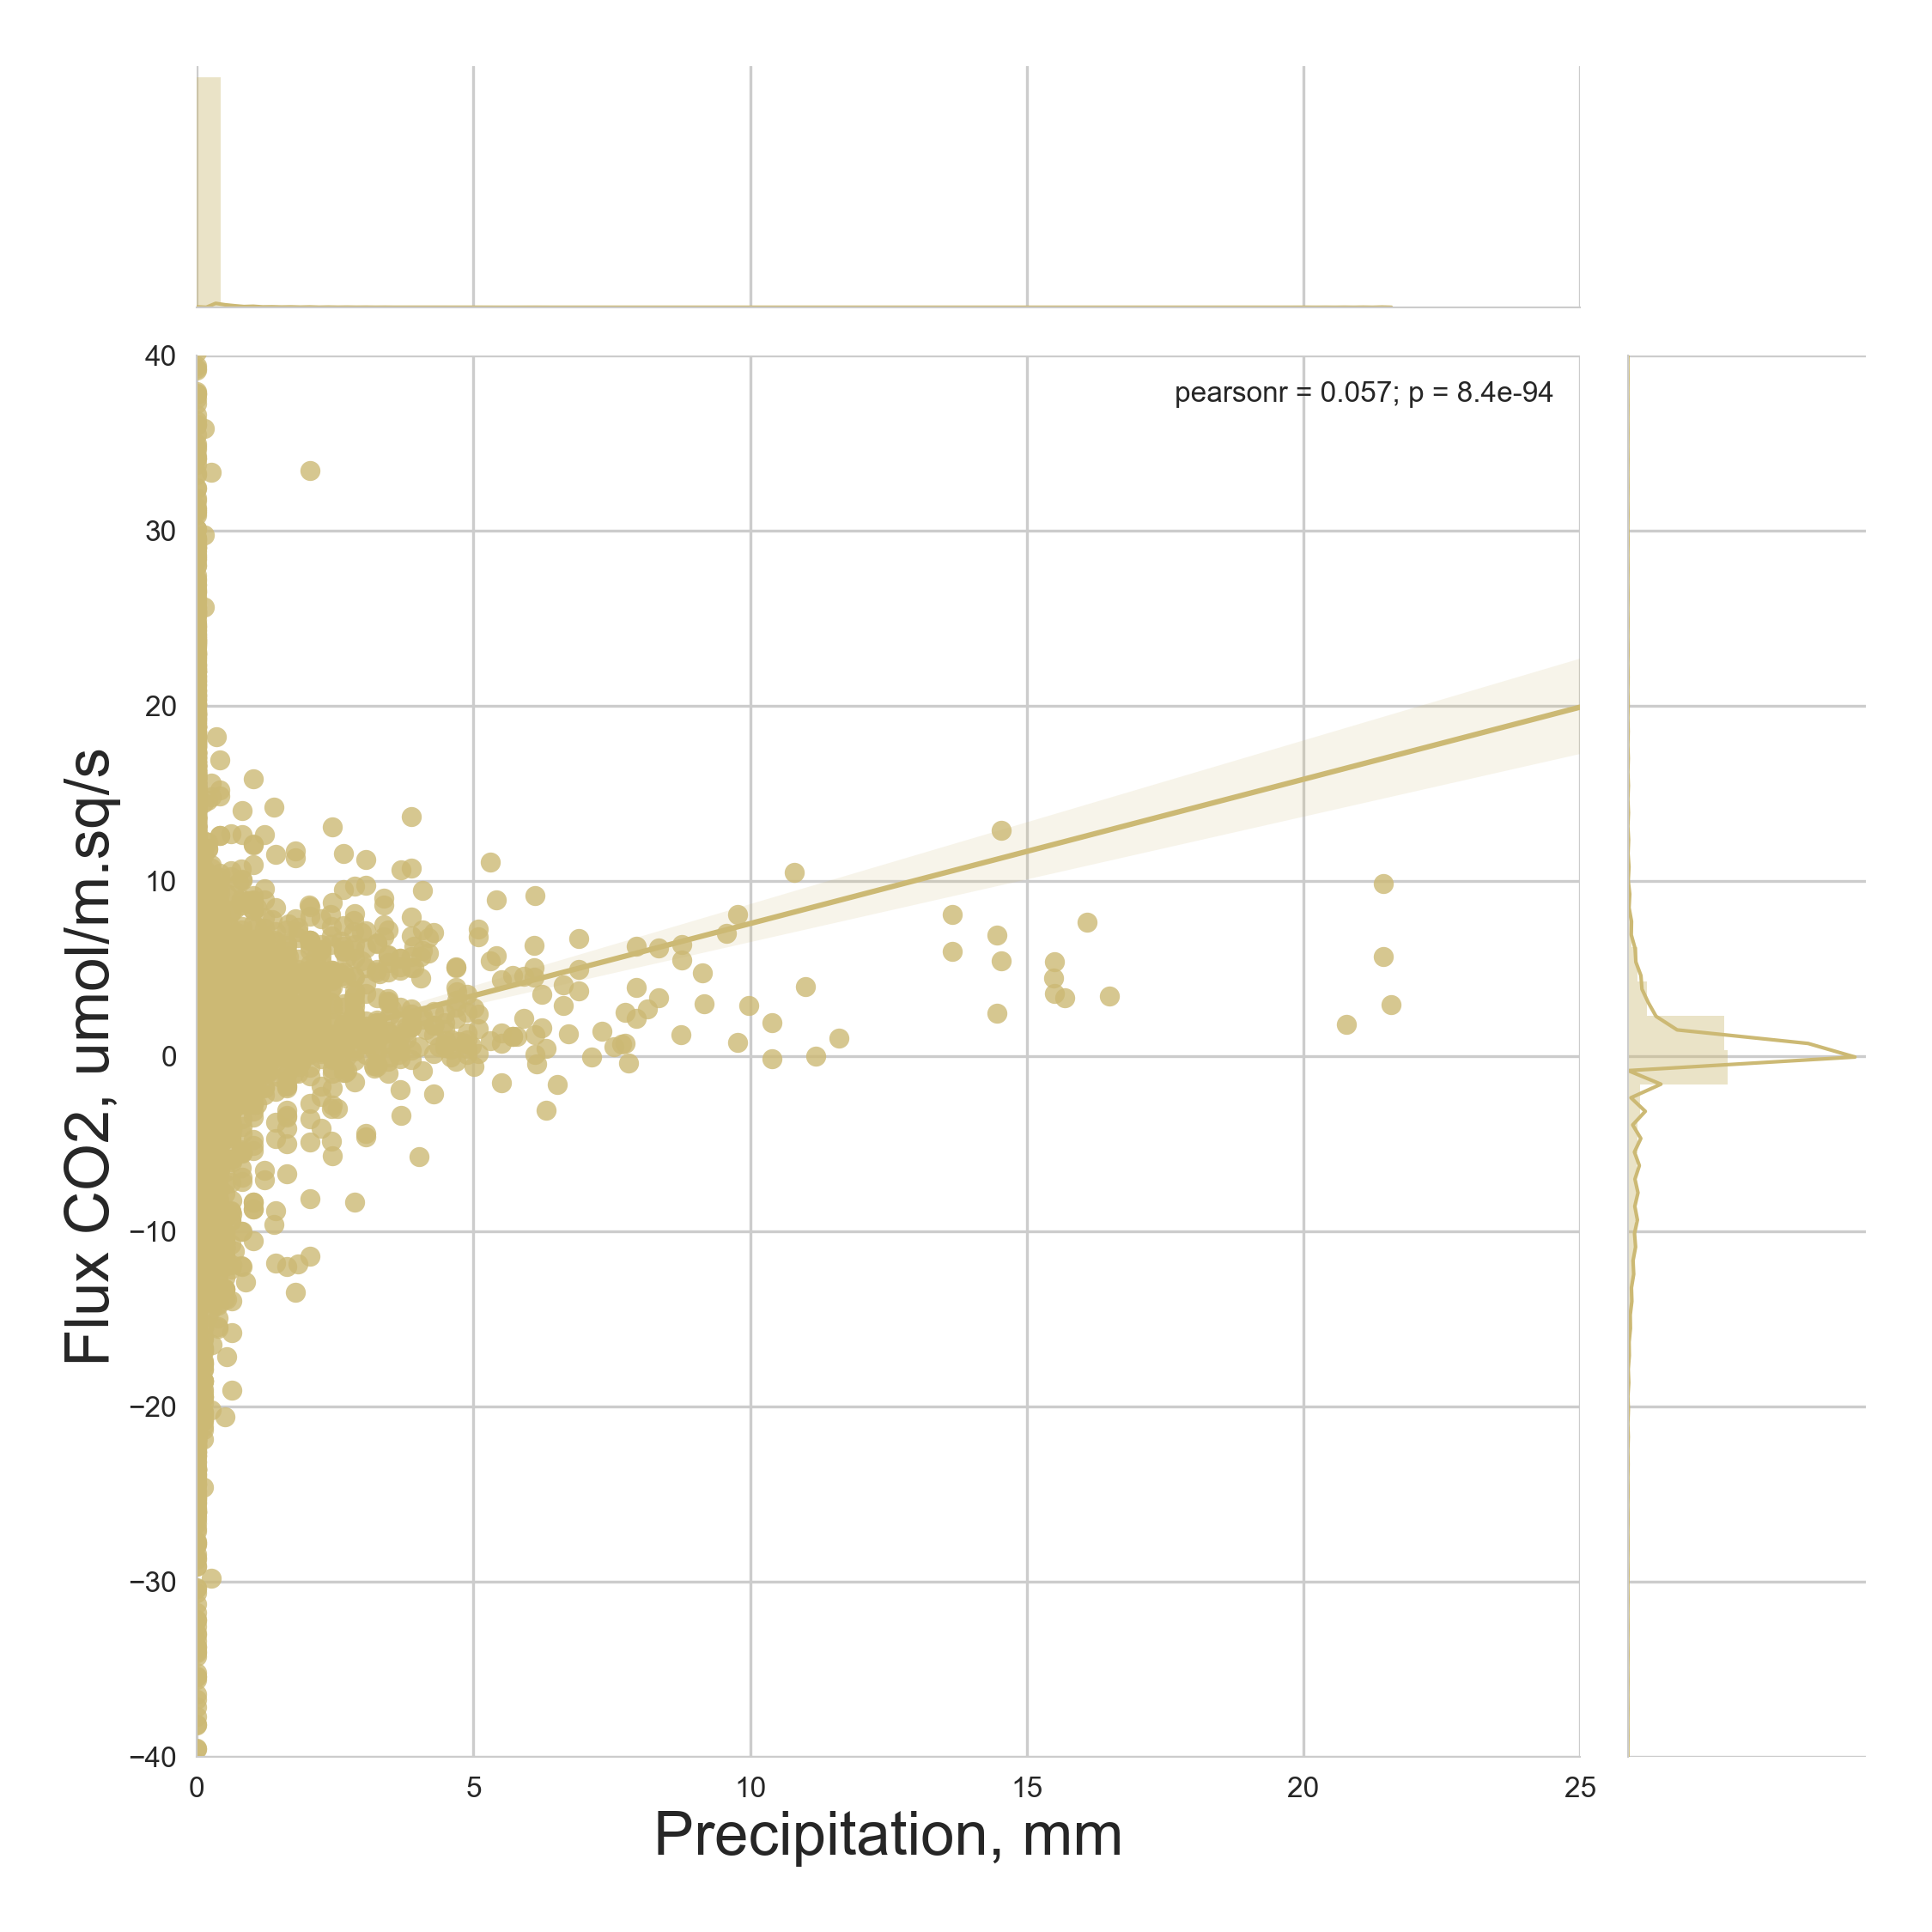
\includegraphics[width=\textwidth]{FvsP/US-Los.png}
\end{columns}

\end{frame}

\begin{frame}
\frametitle{Flux vs Soil Water Content}

\begin{columns}[t]
\column{.35\textwidth}
\centering
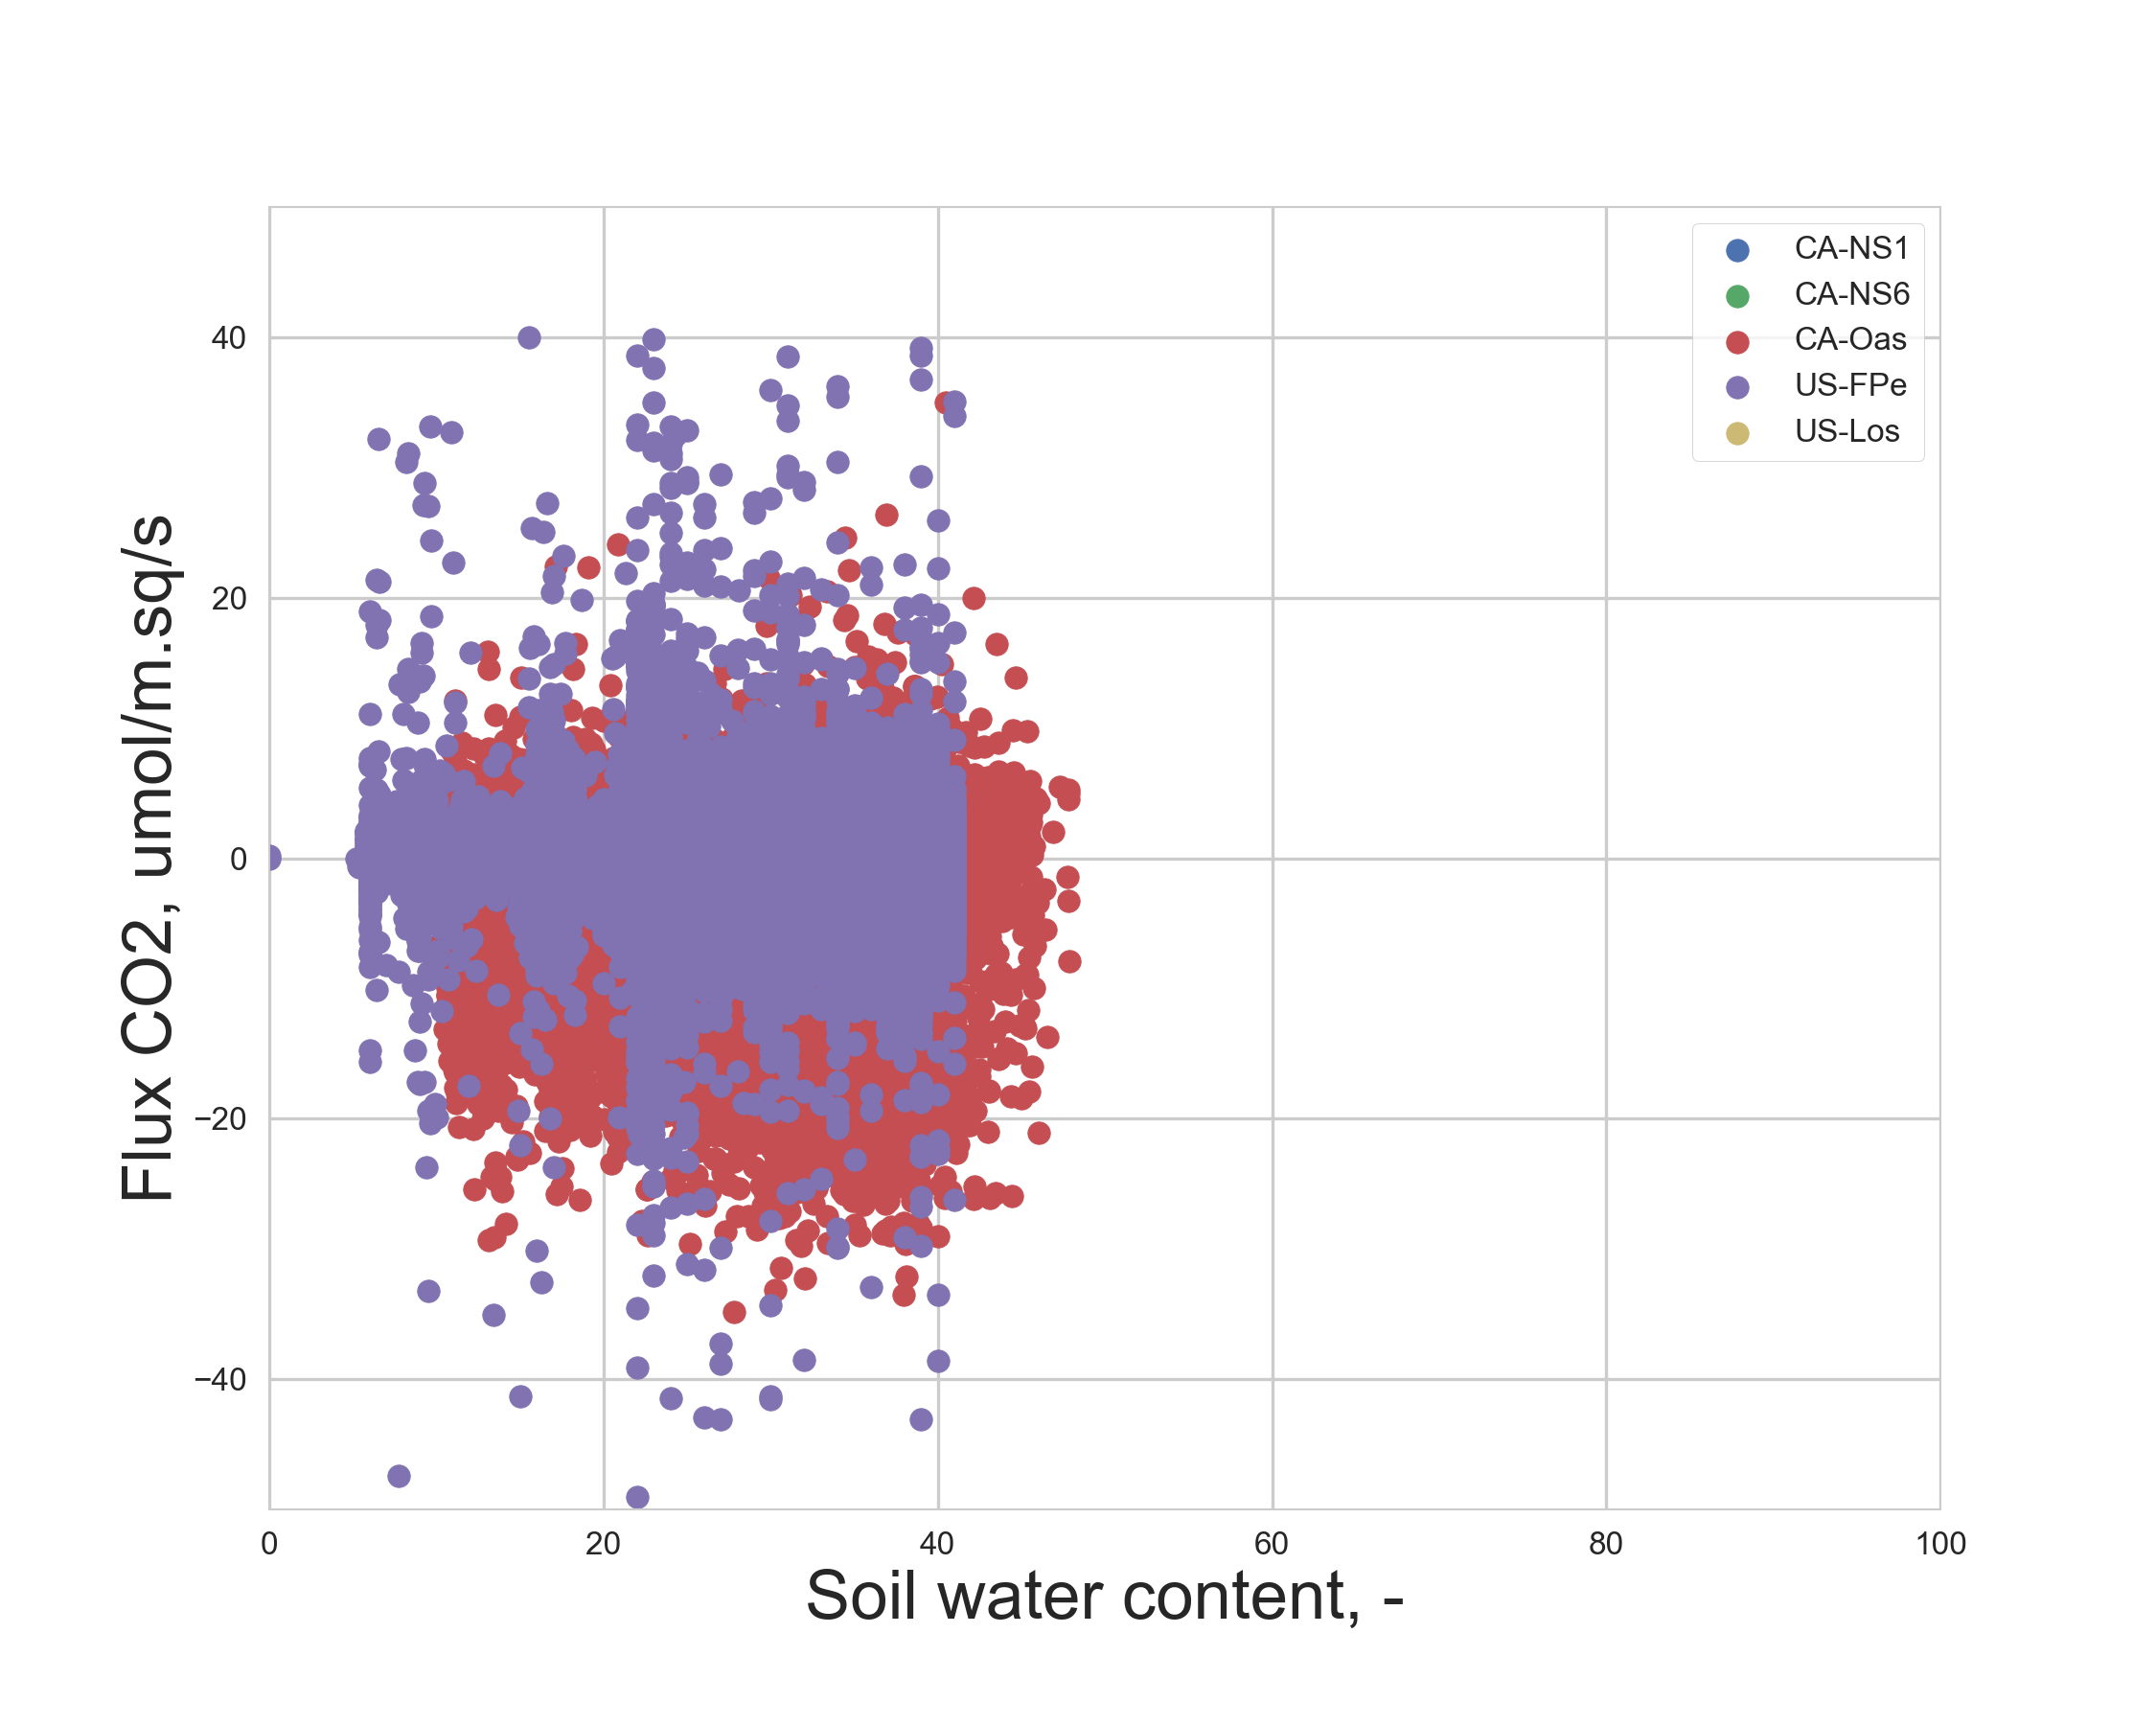
\includegraphics[width=\textwidth]{FvsSWC/all.png}\\
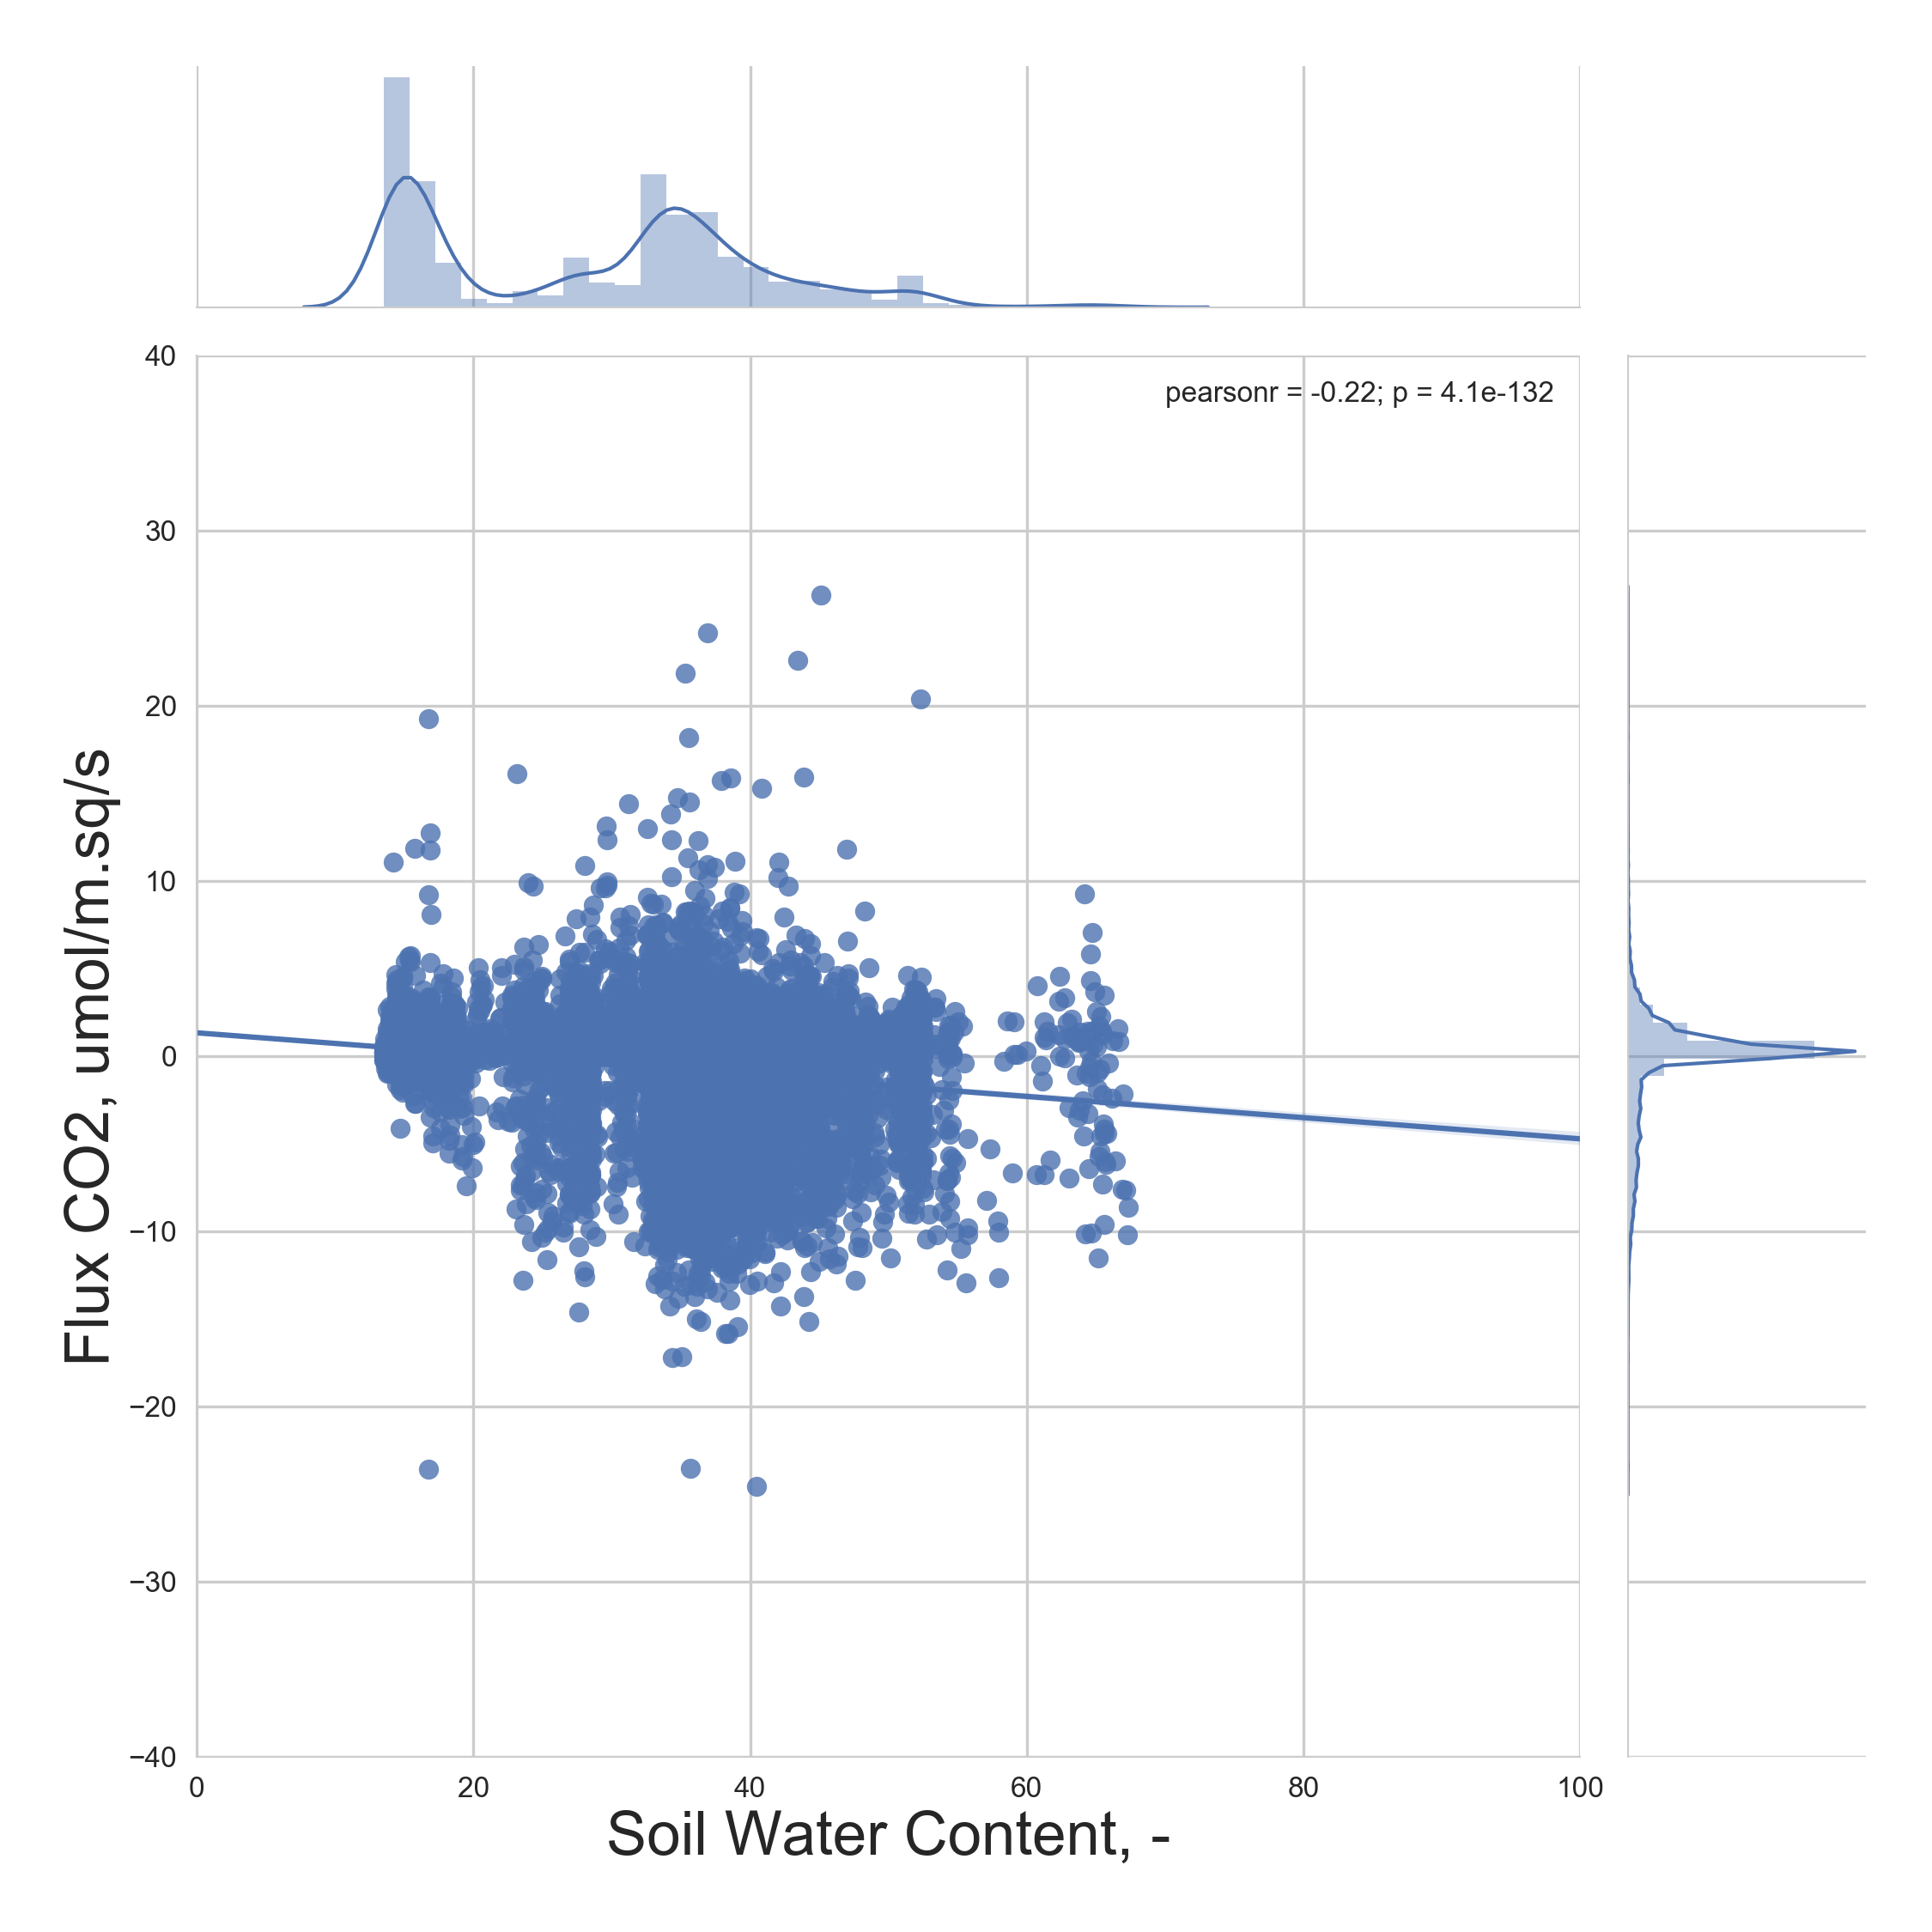
\includegraphics[width=\textwidth]{FvsSWC/CA-NS1.png}
\column{.35\textwidth}
\centering
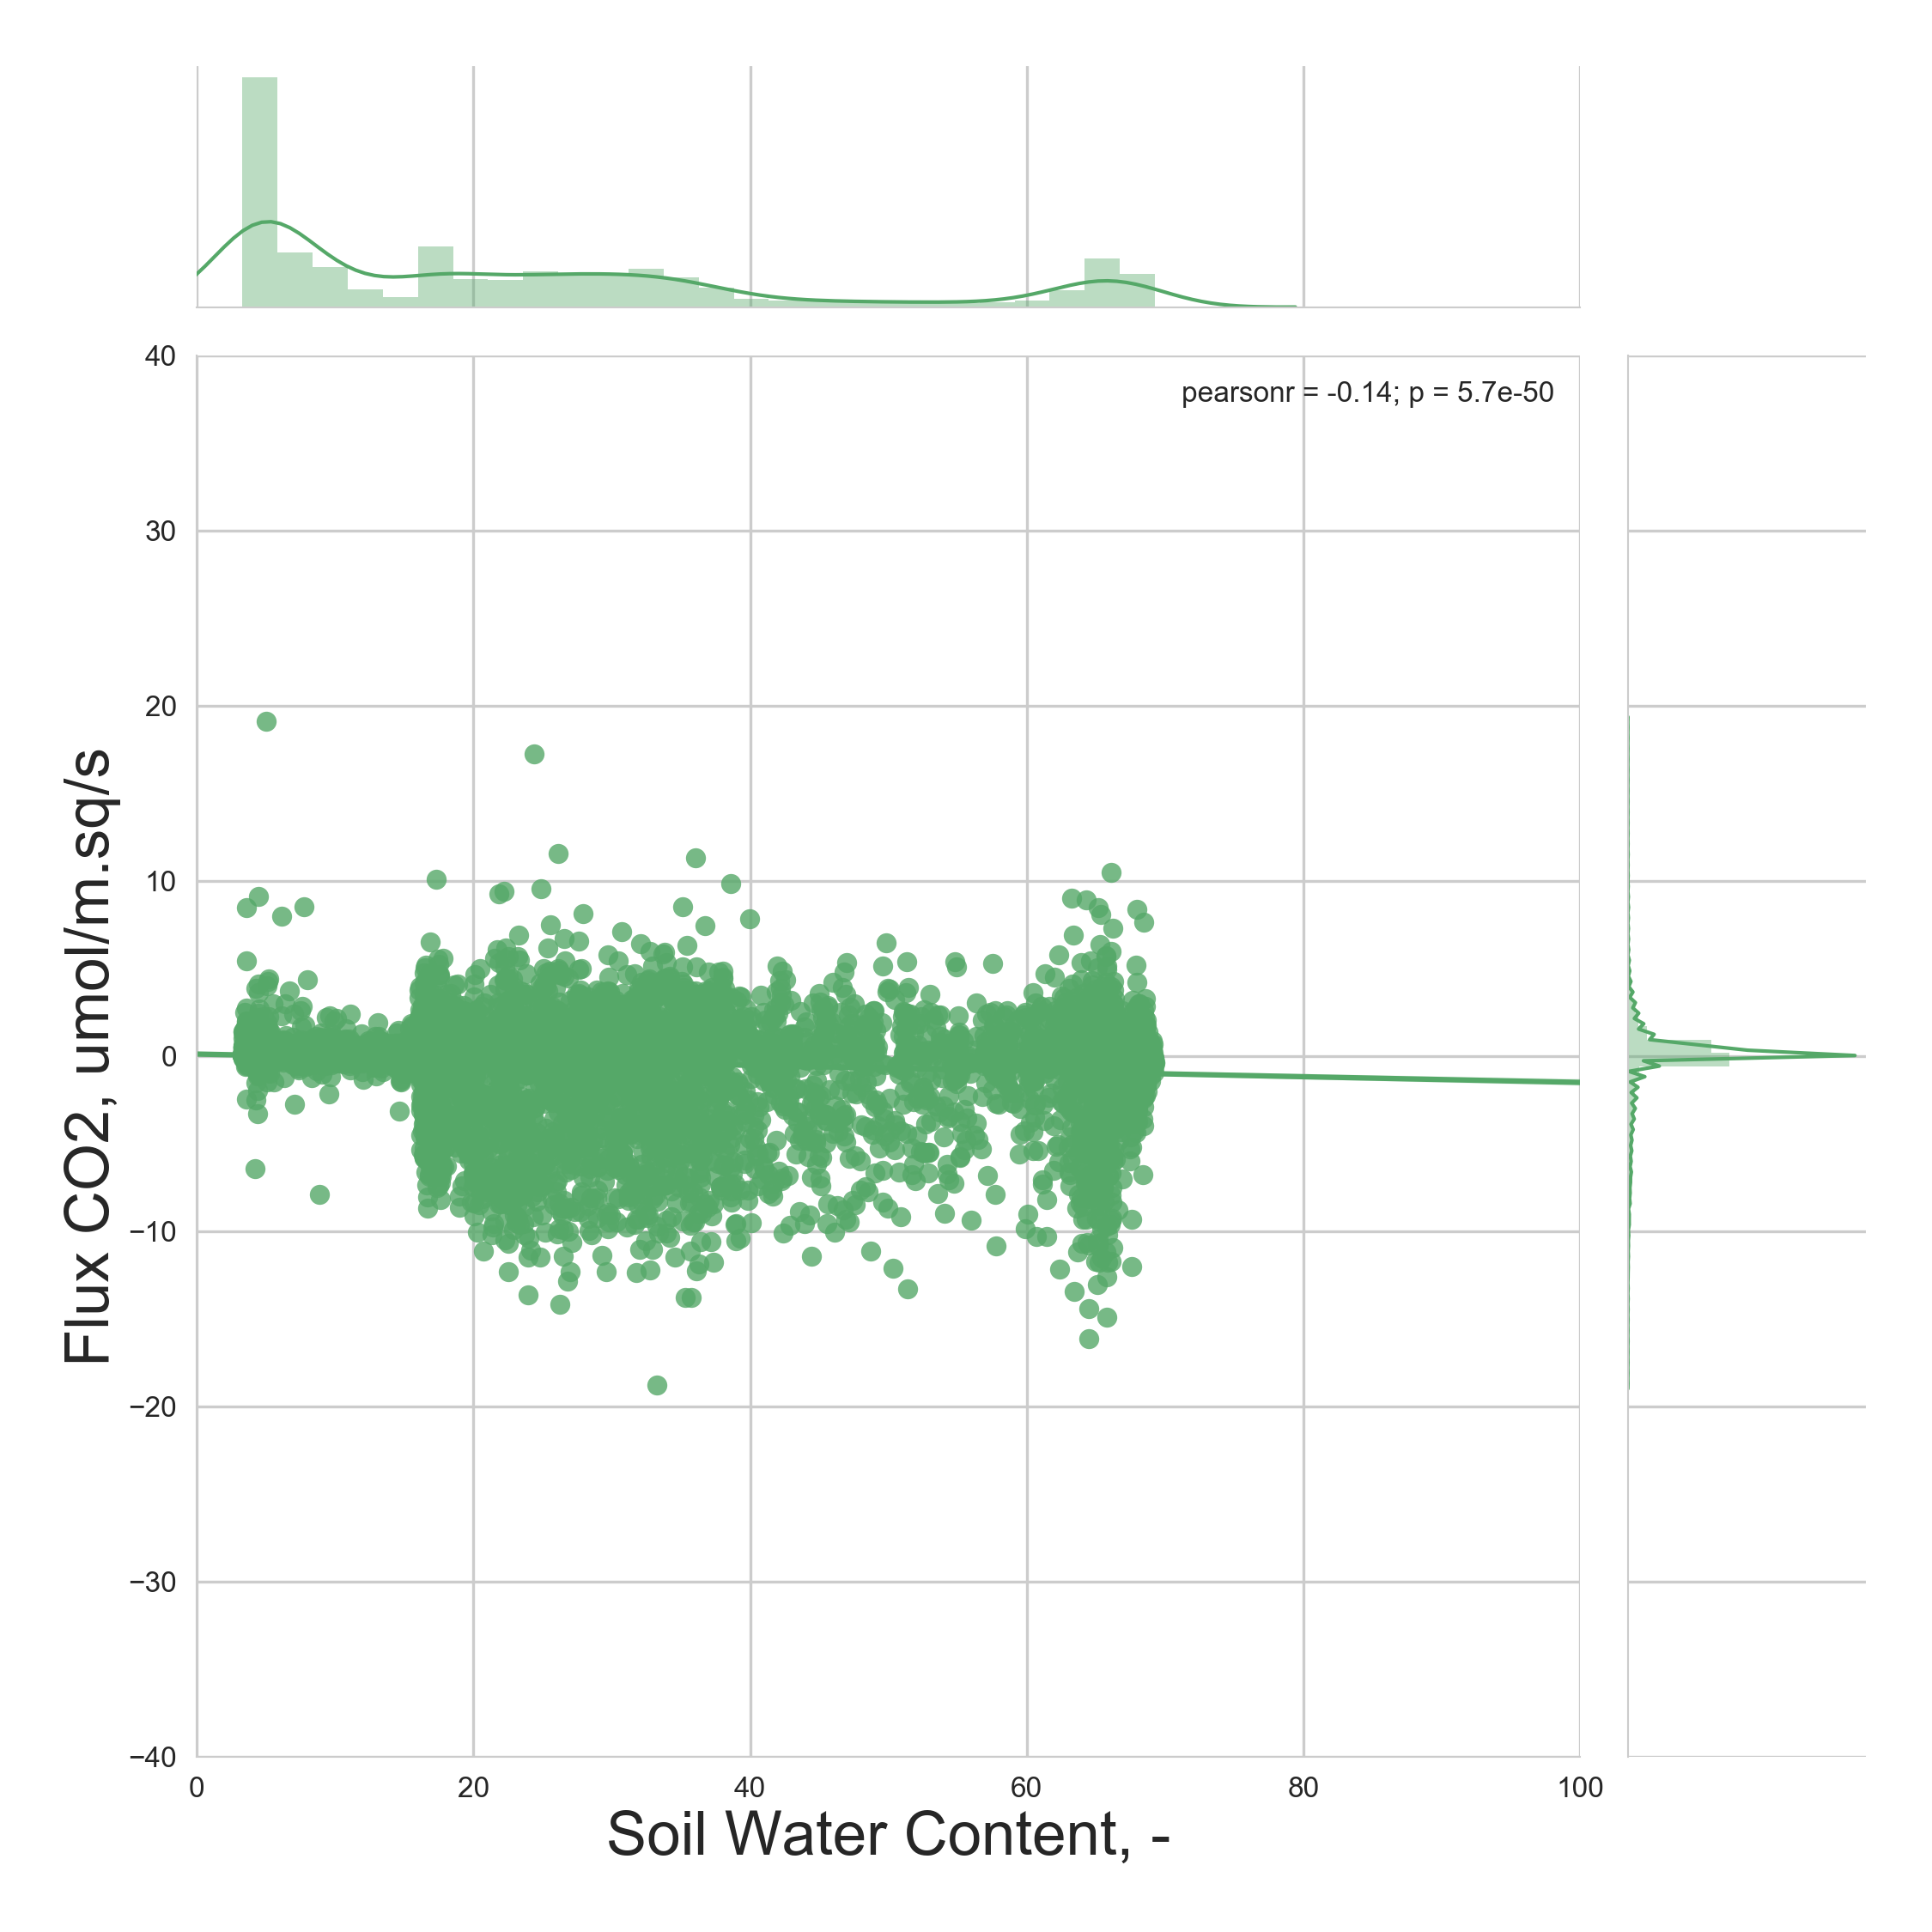
\includegraphics[width=\textwidth]{FvsSWC/CA-NS6.png}\\
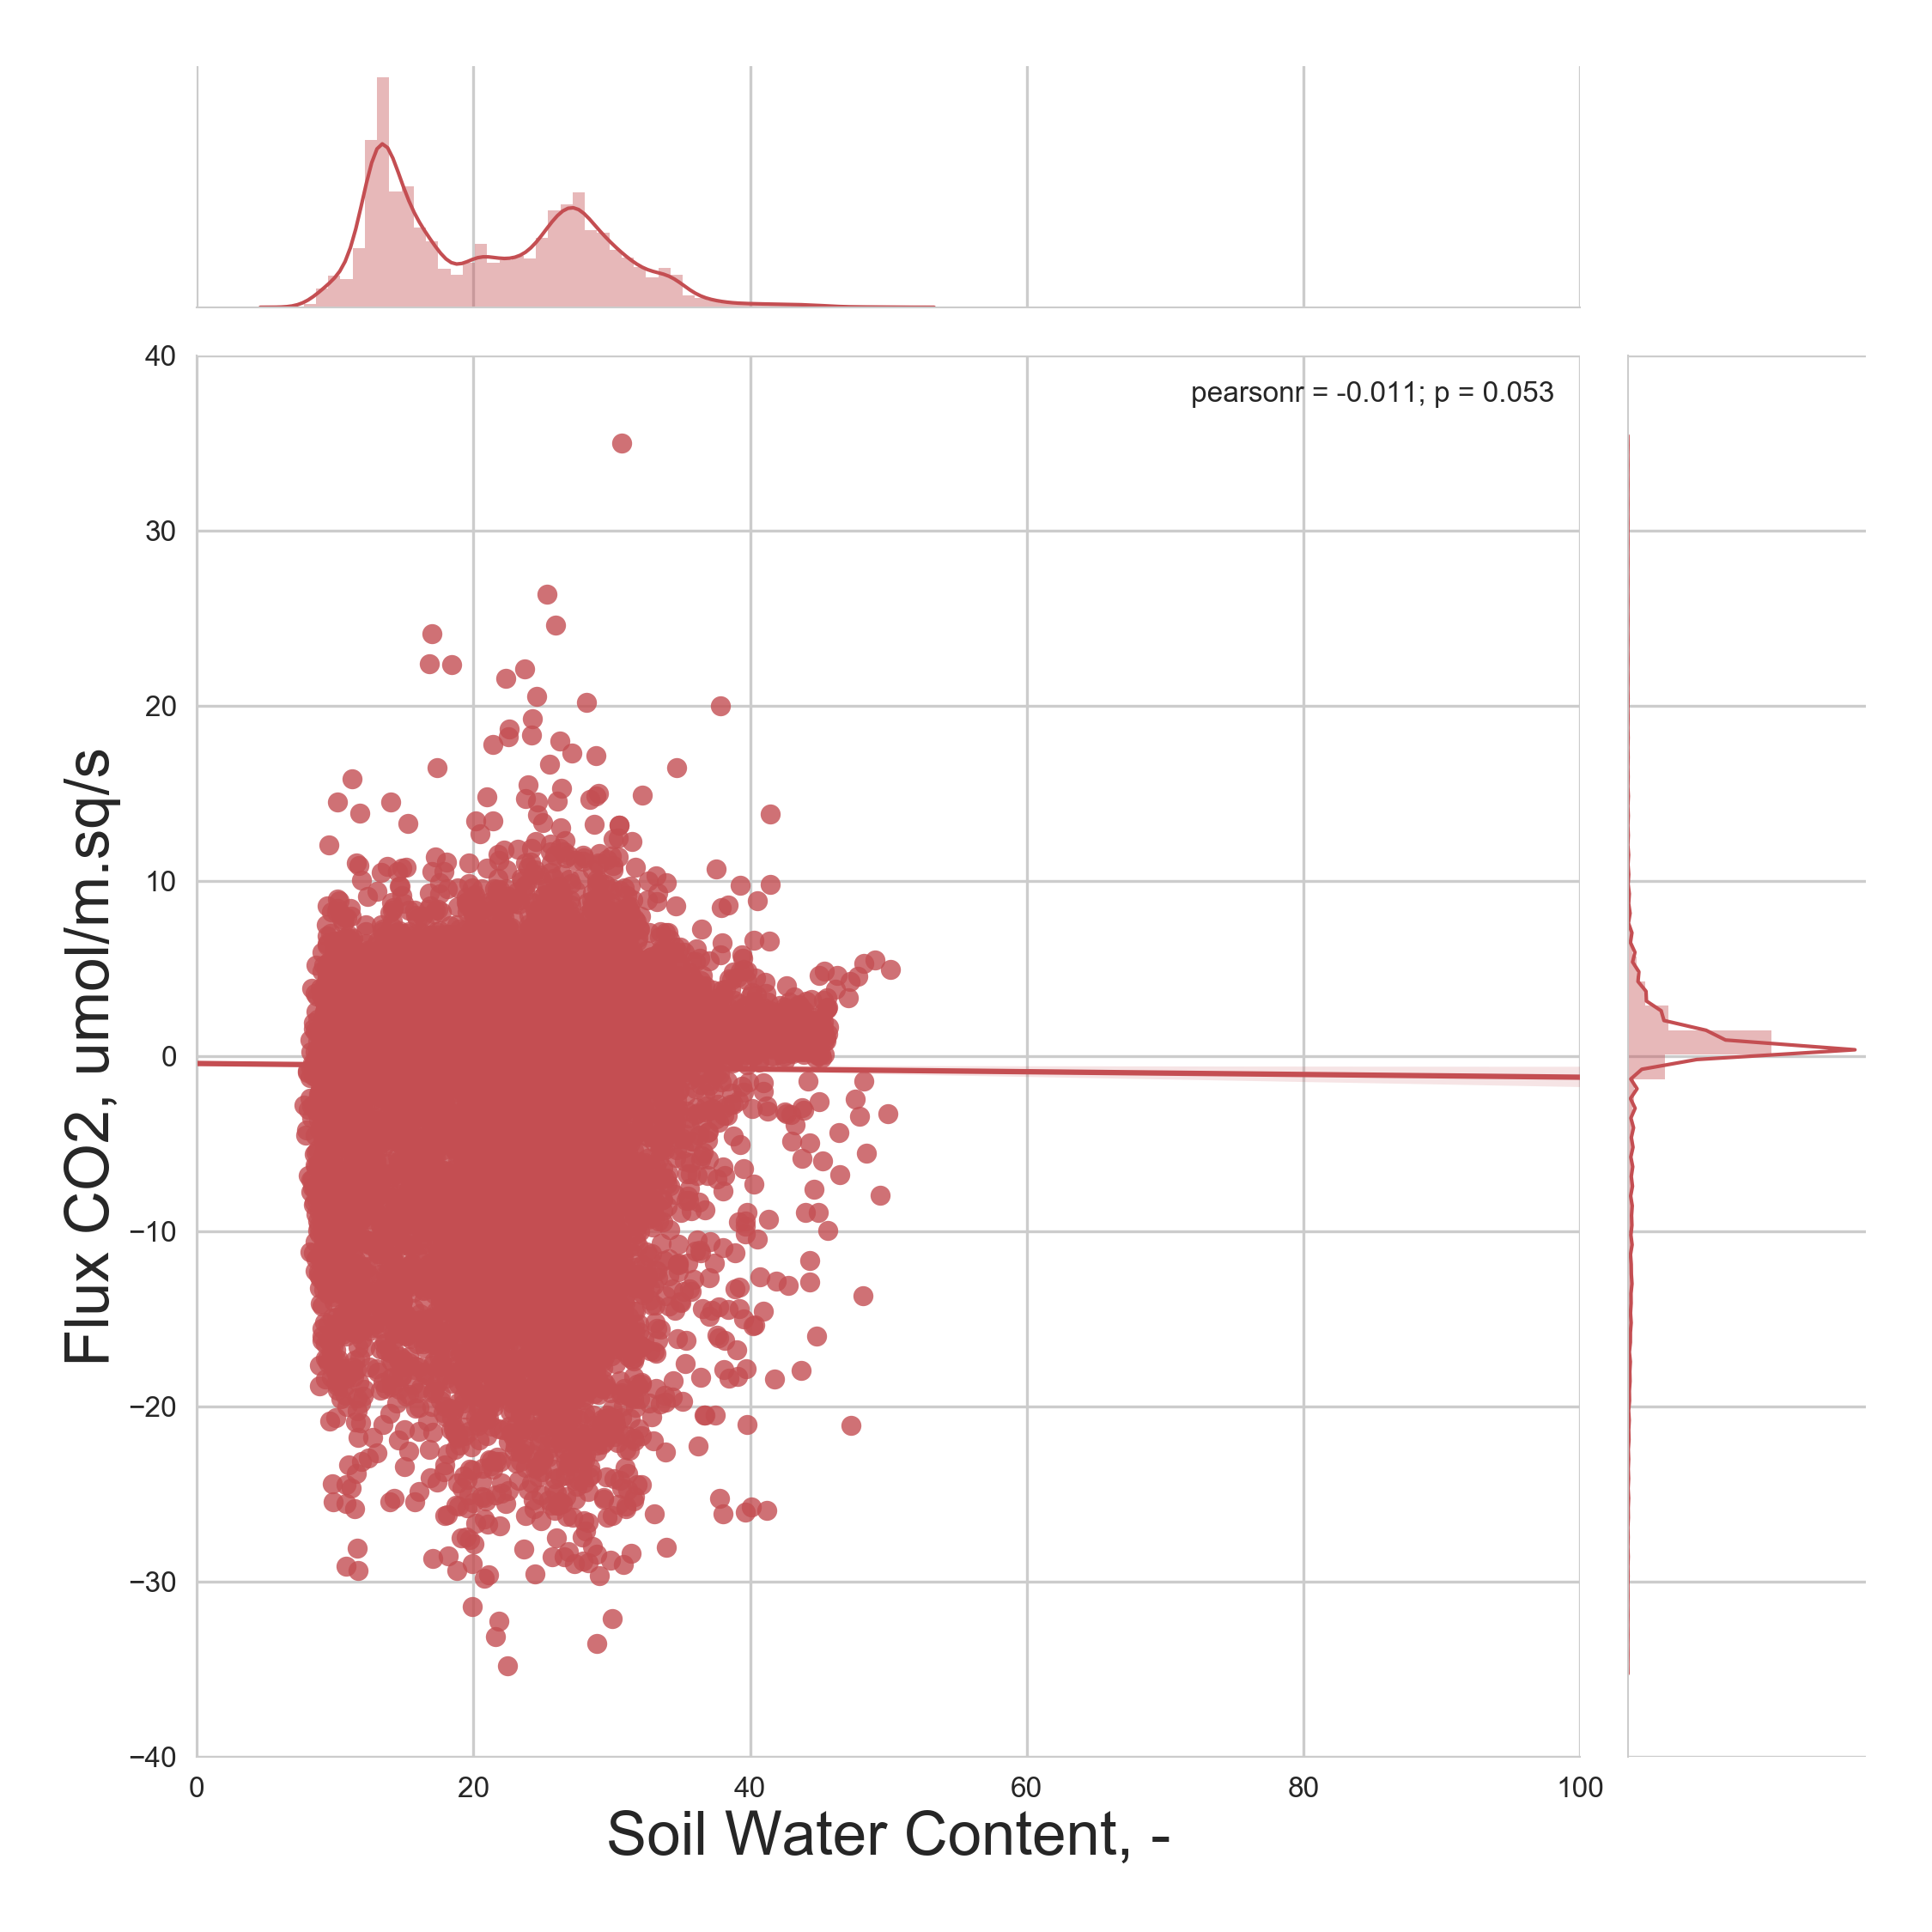
\includegraphics[width=\textwidth]{FvsSWC/CA-Oas.png}
\column{.35\textwidth}
\centering
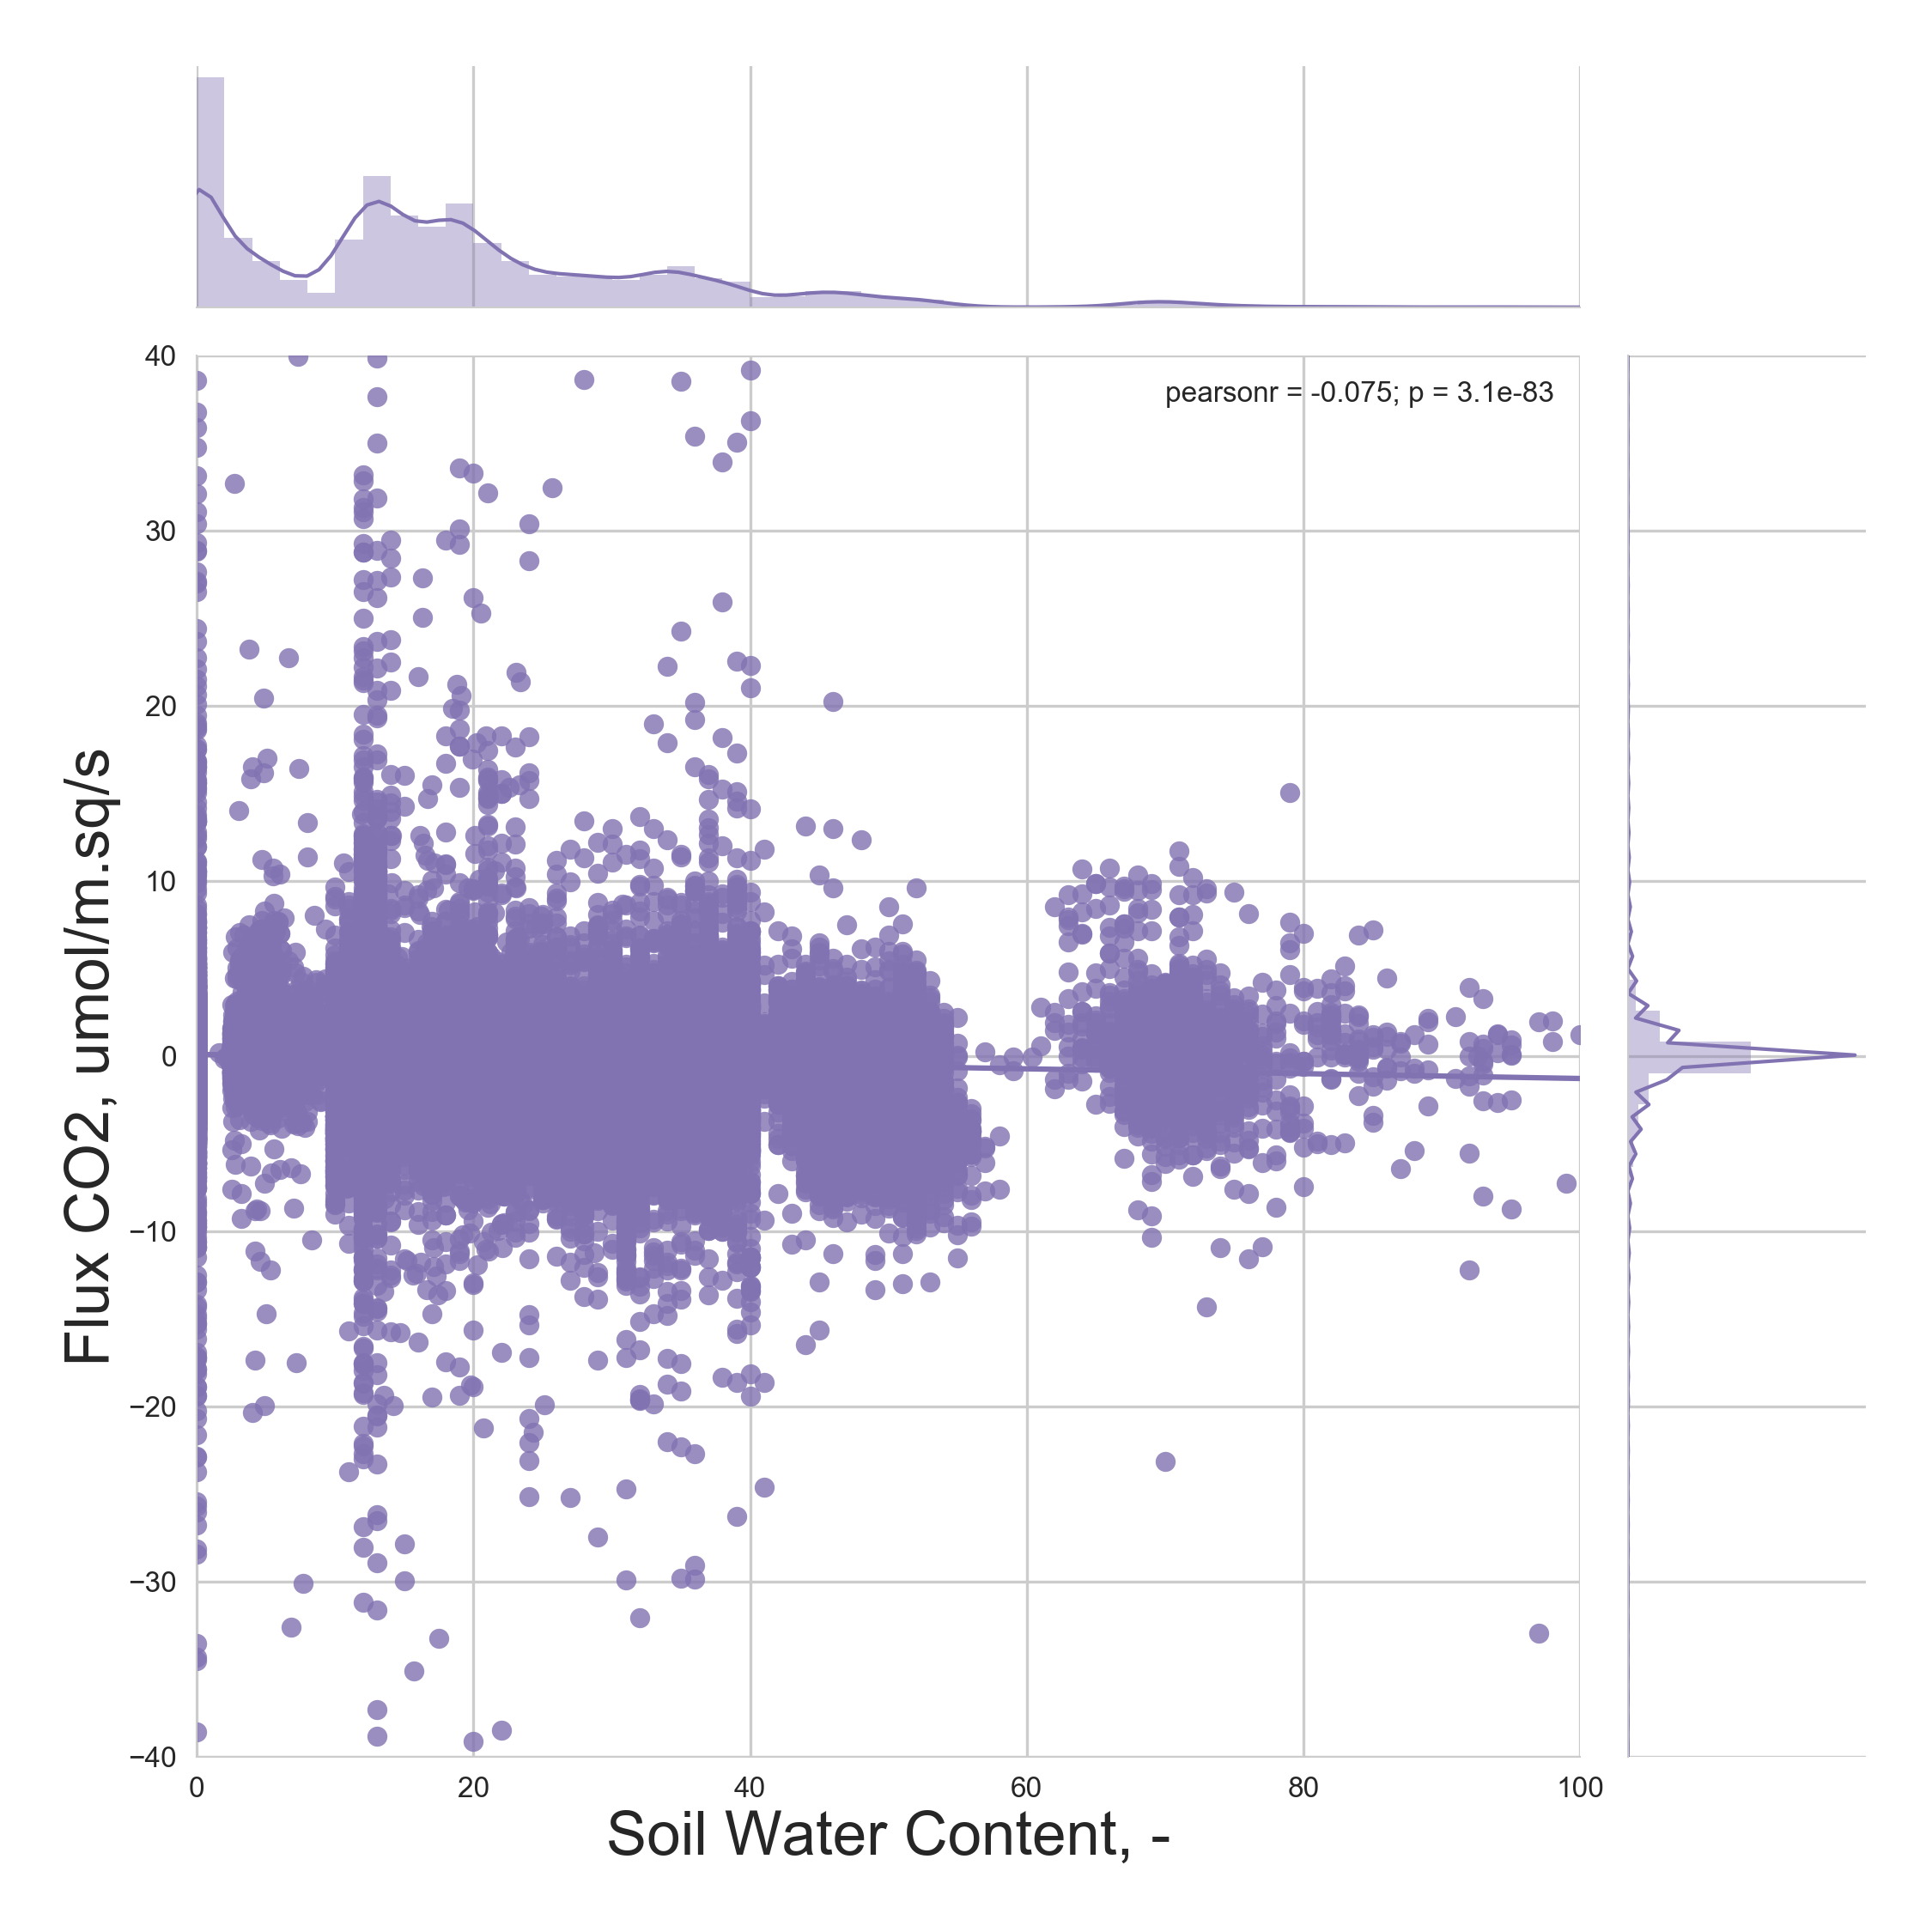
\includegraphics[width=\textwidth]{FvsSWC/US-FPe.png}\\
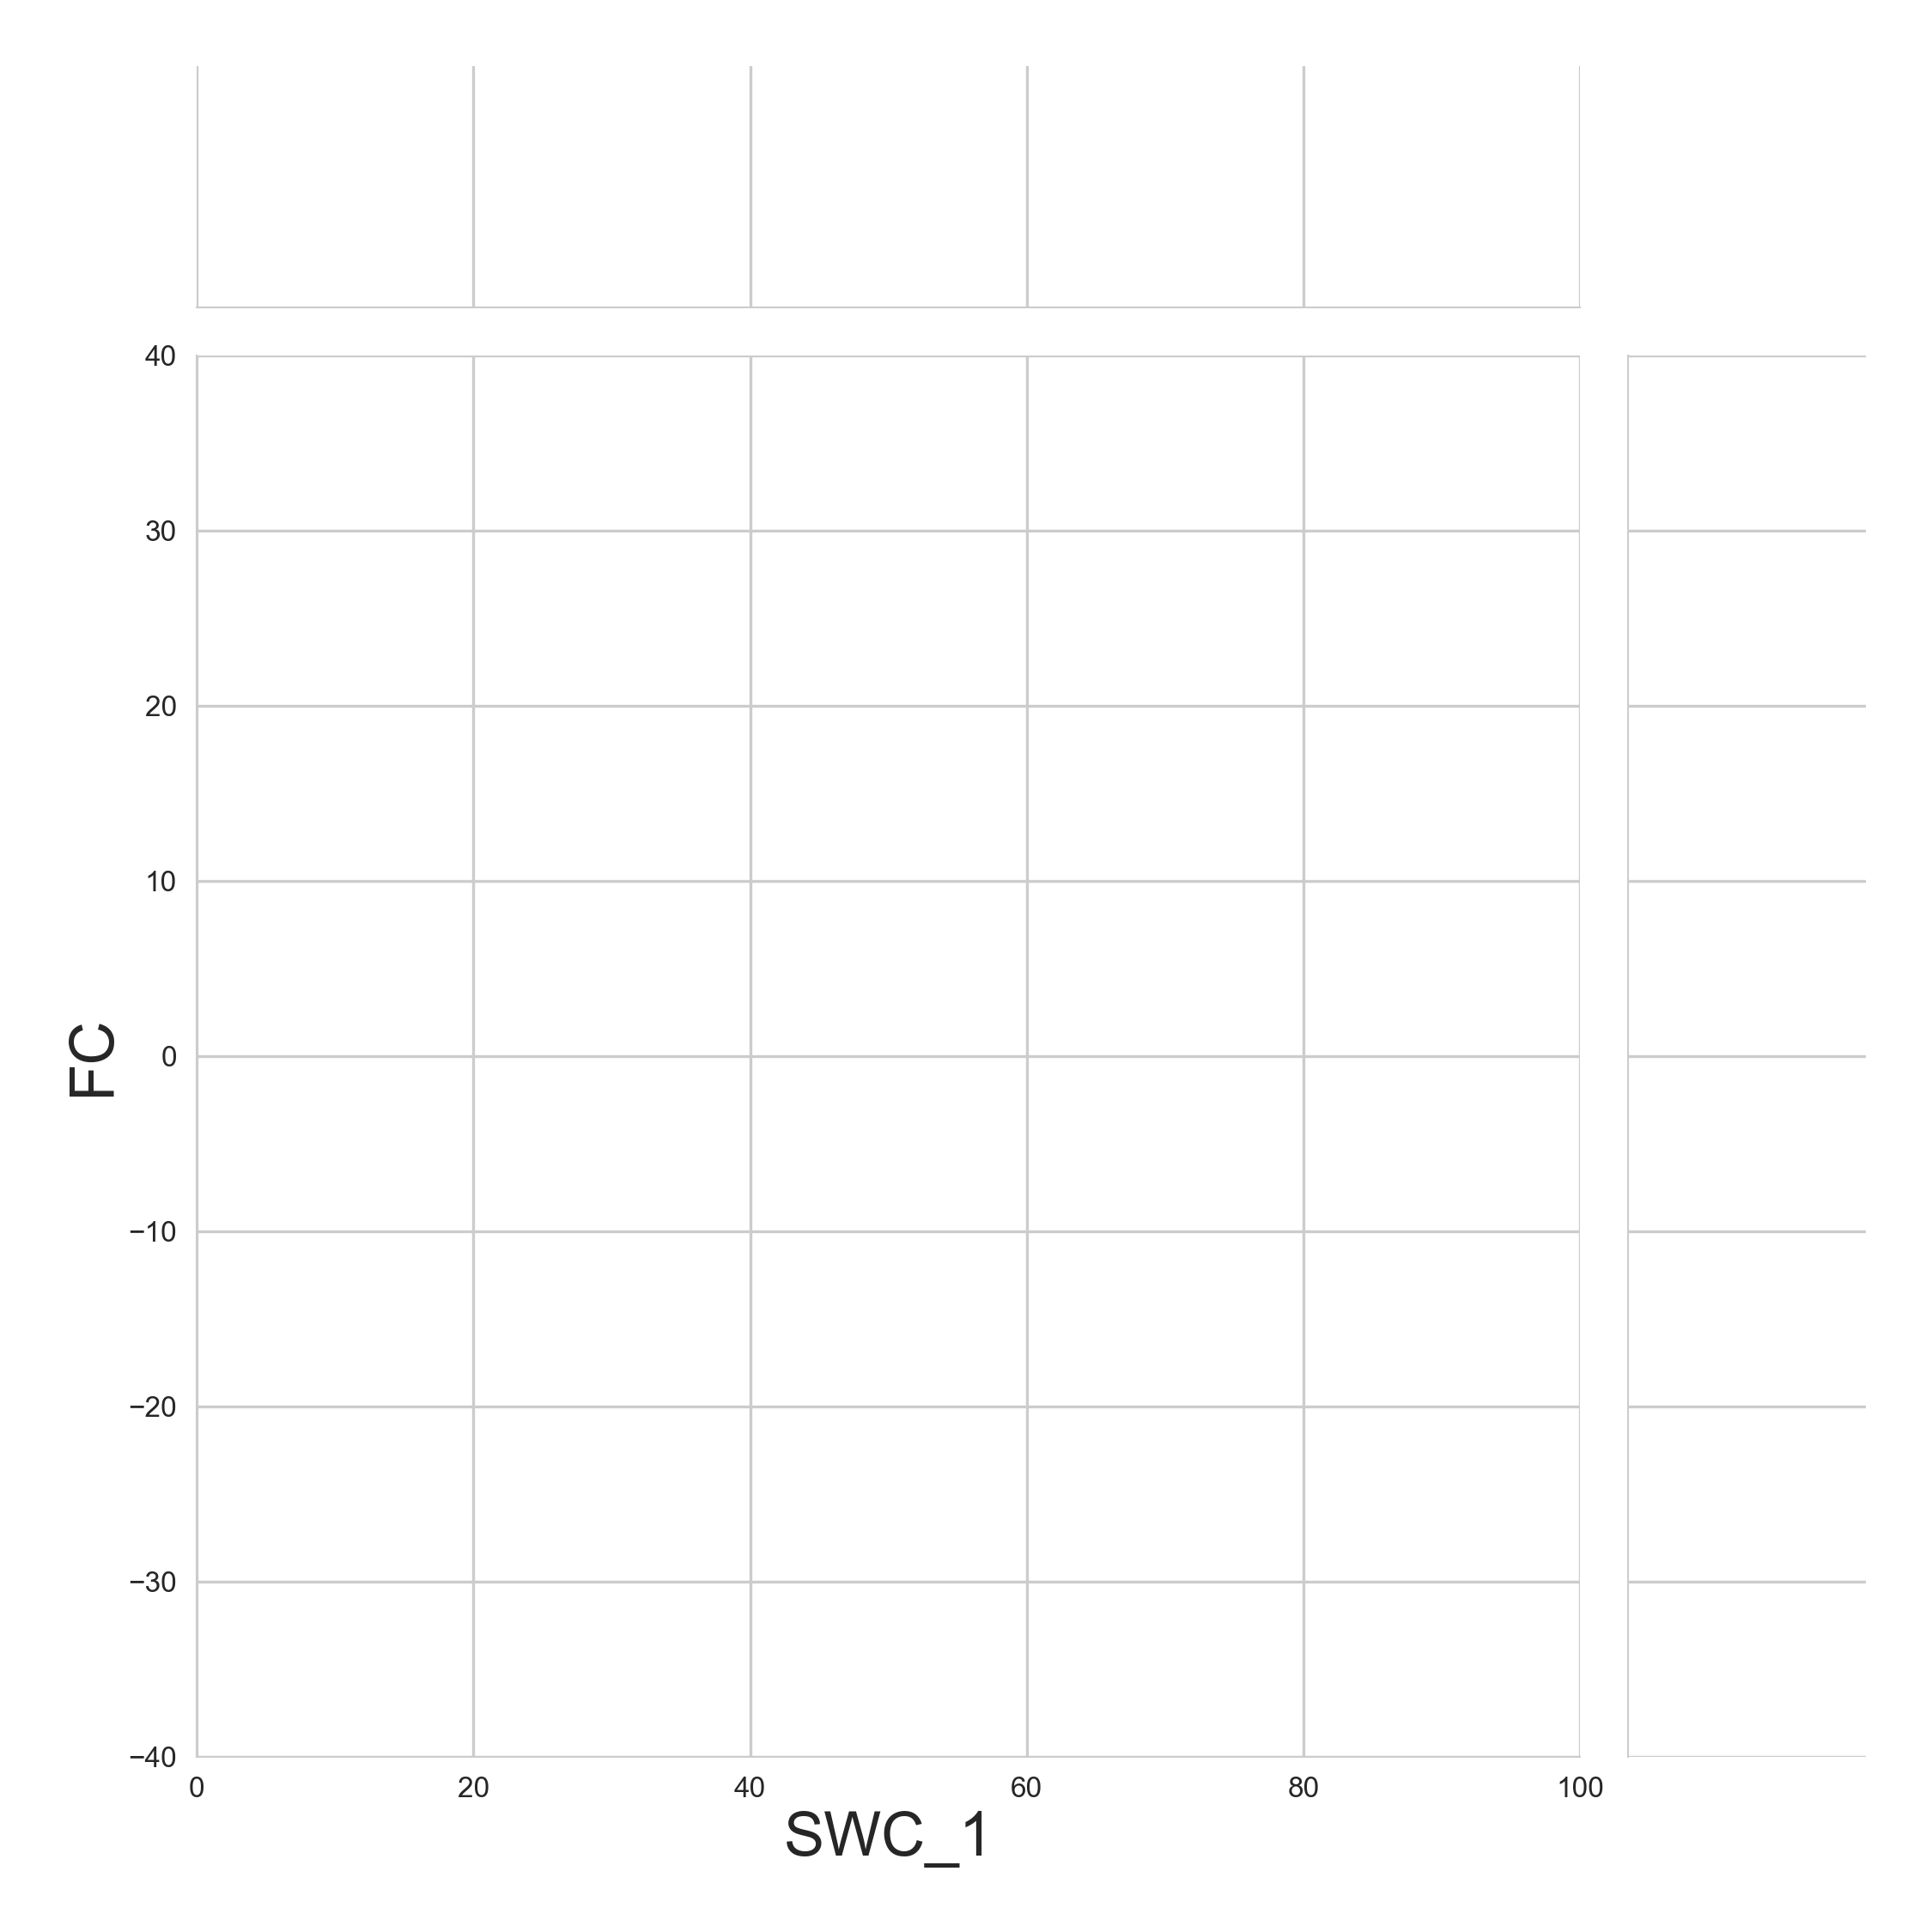
\includegraphics[width=\textwidth]{FvsSWC/US-Los.png}
\end{columns}

\end{frame}

\begin{frame}
\frametitle{Flux on Yearly scale}

\begin{columns}[t]
\column{.35\textwidth}
\centering
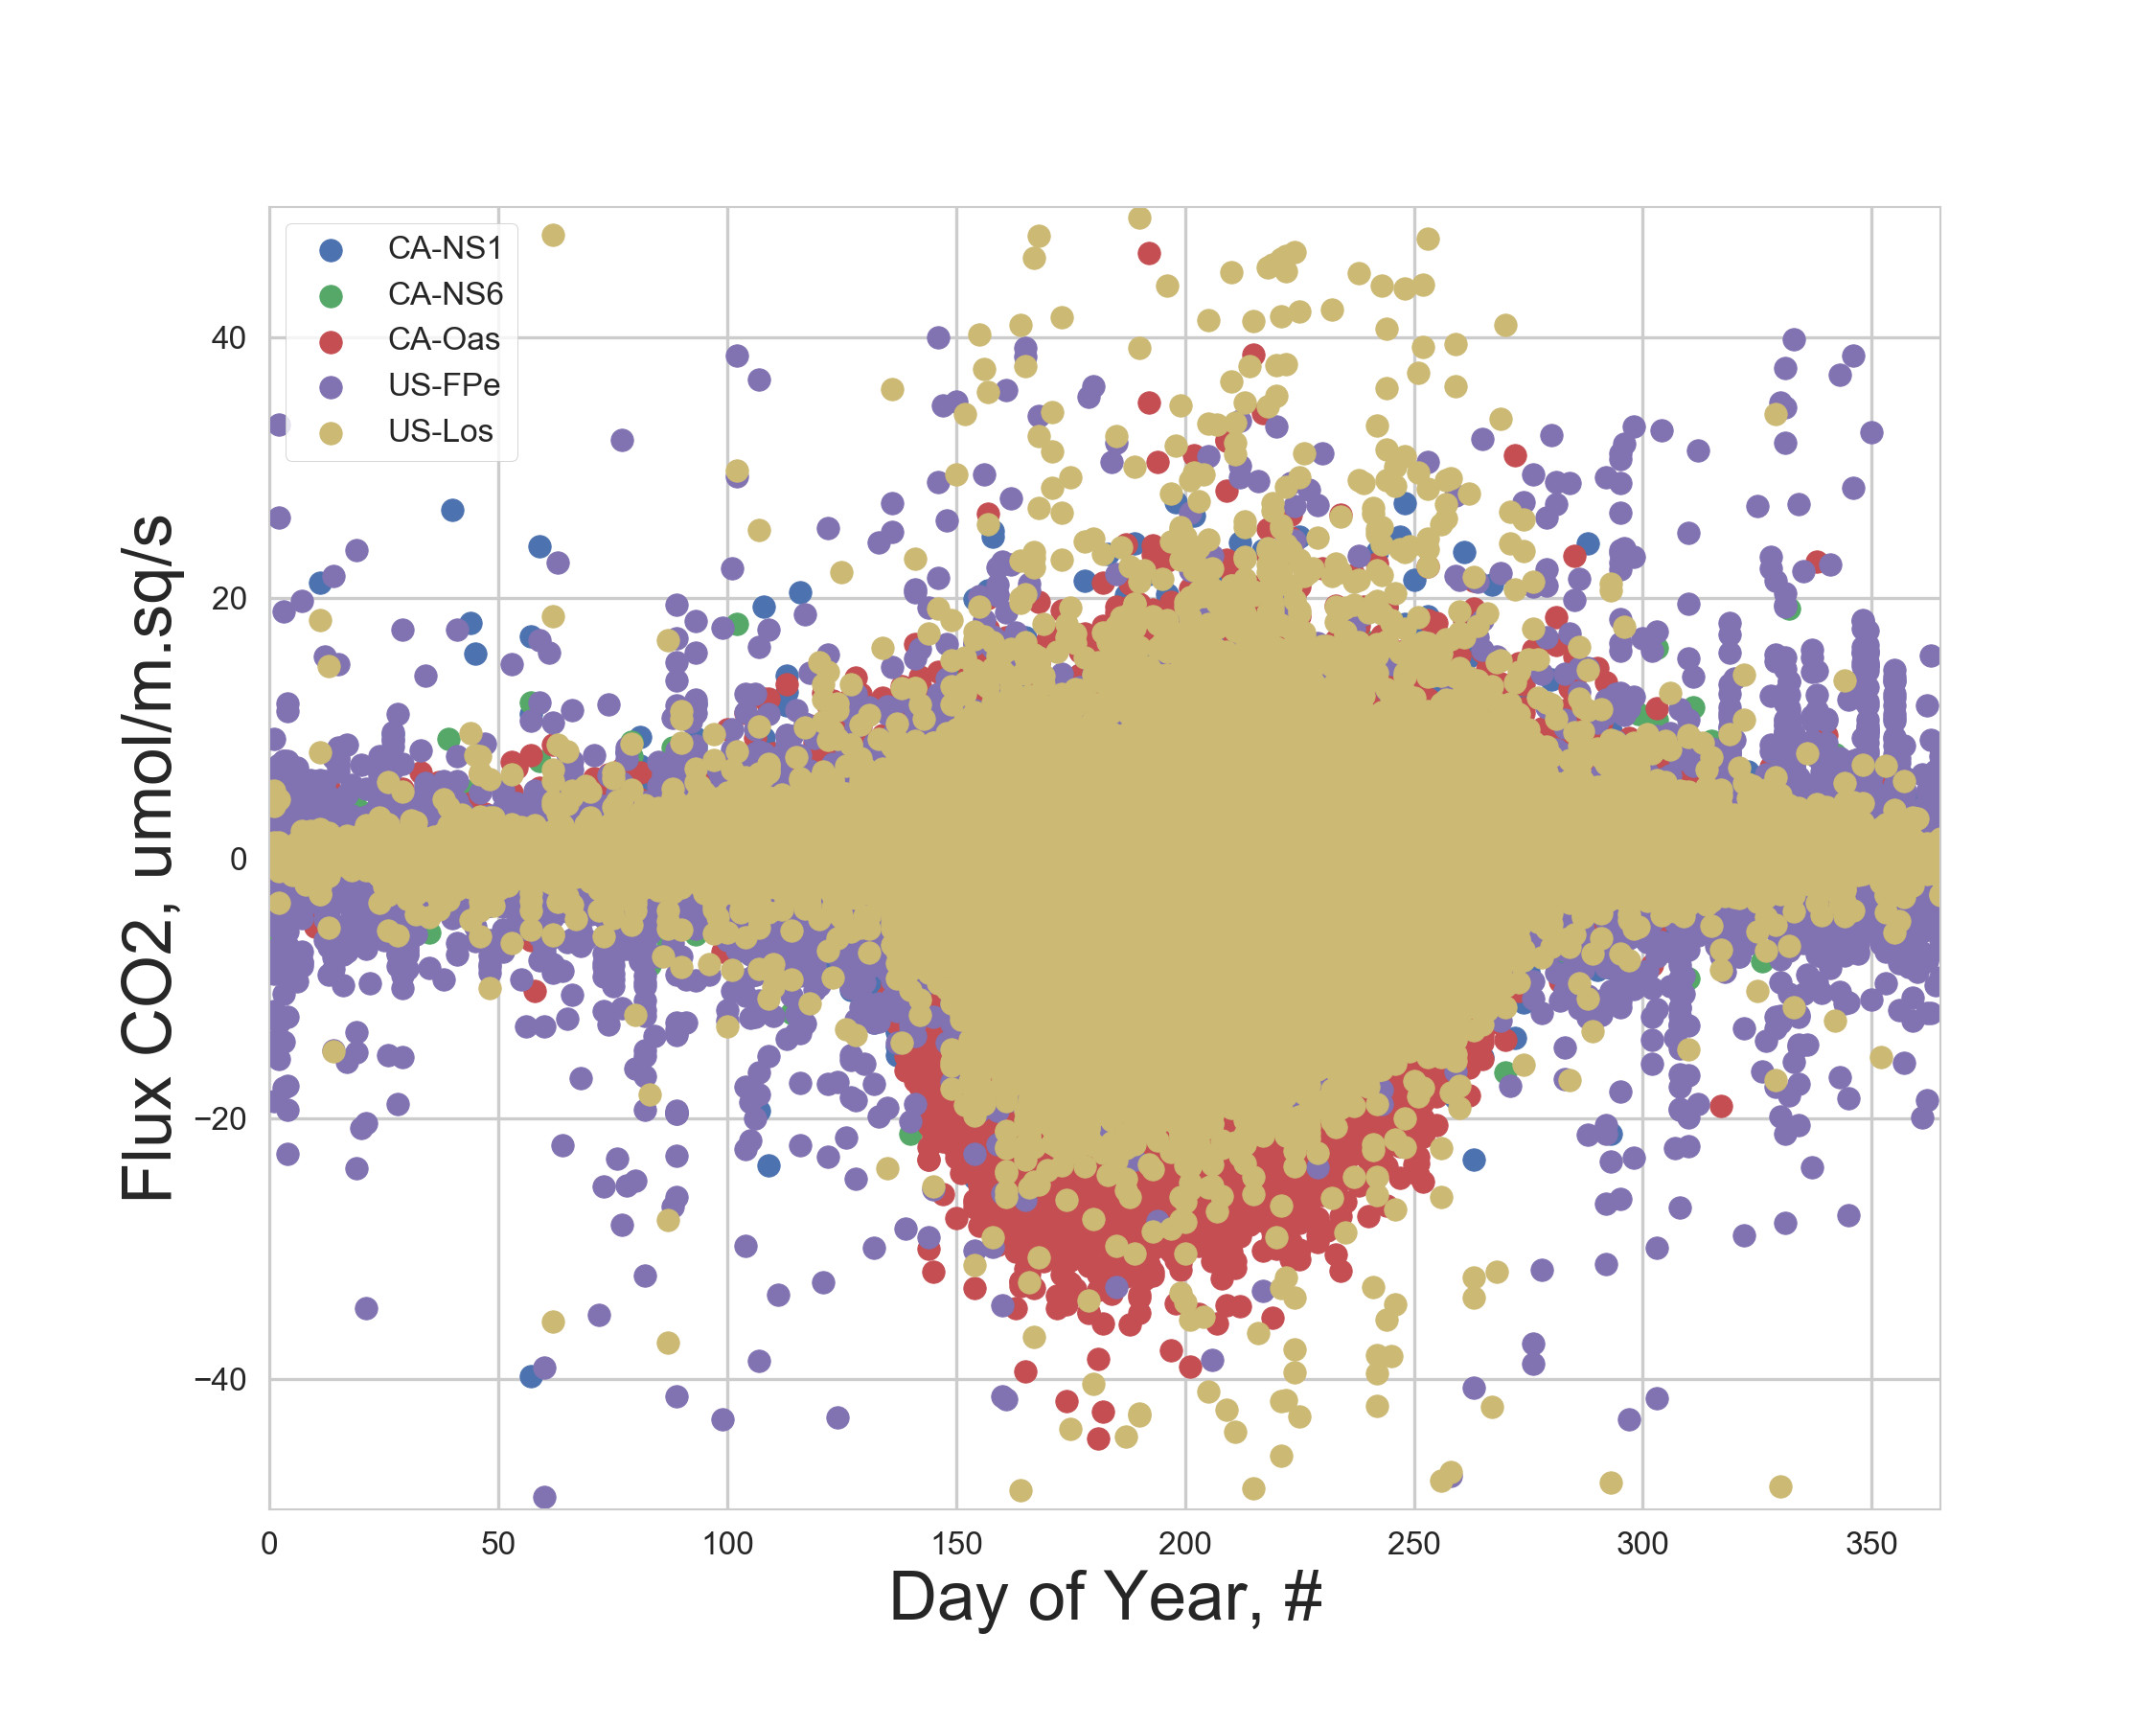
\includegraphics[width=\textwidth]{FvsY/all.png}\\
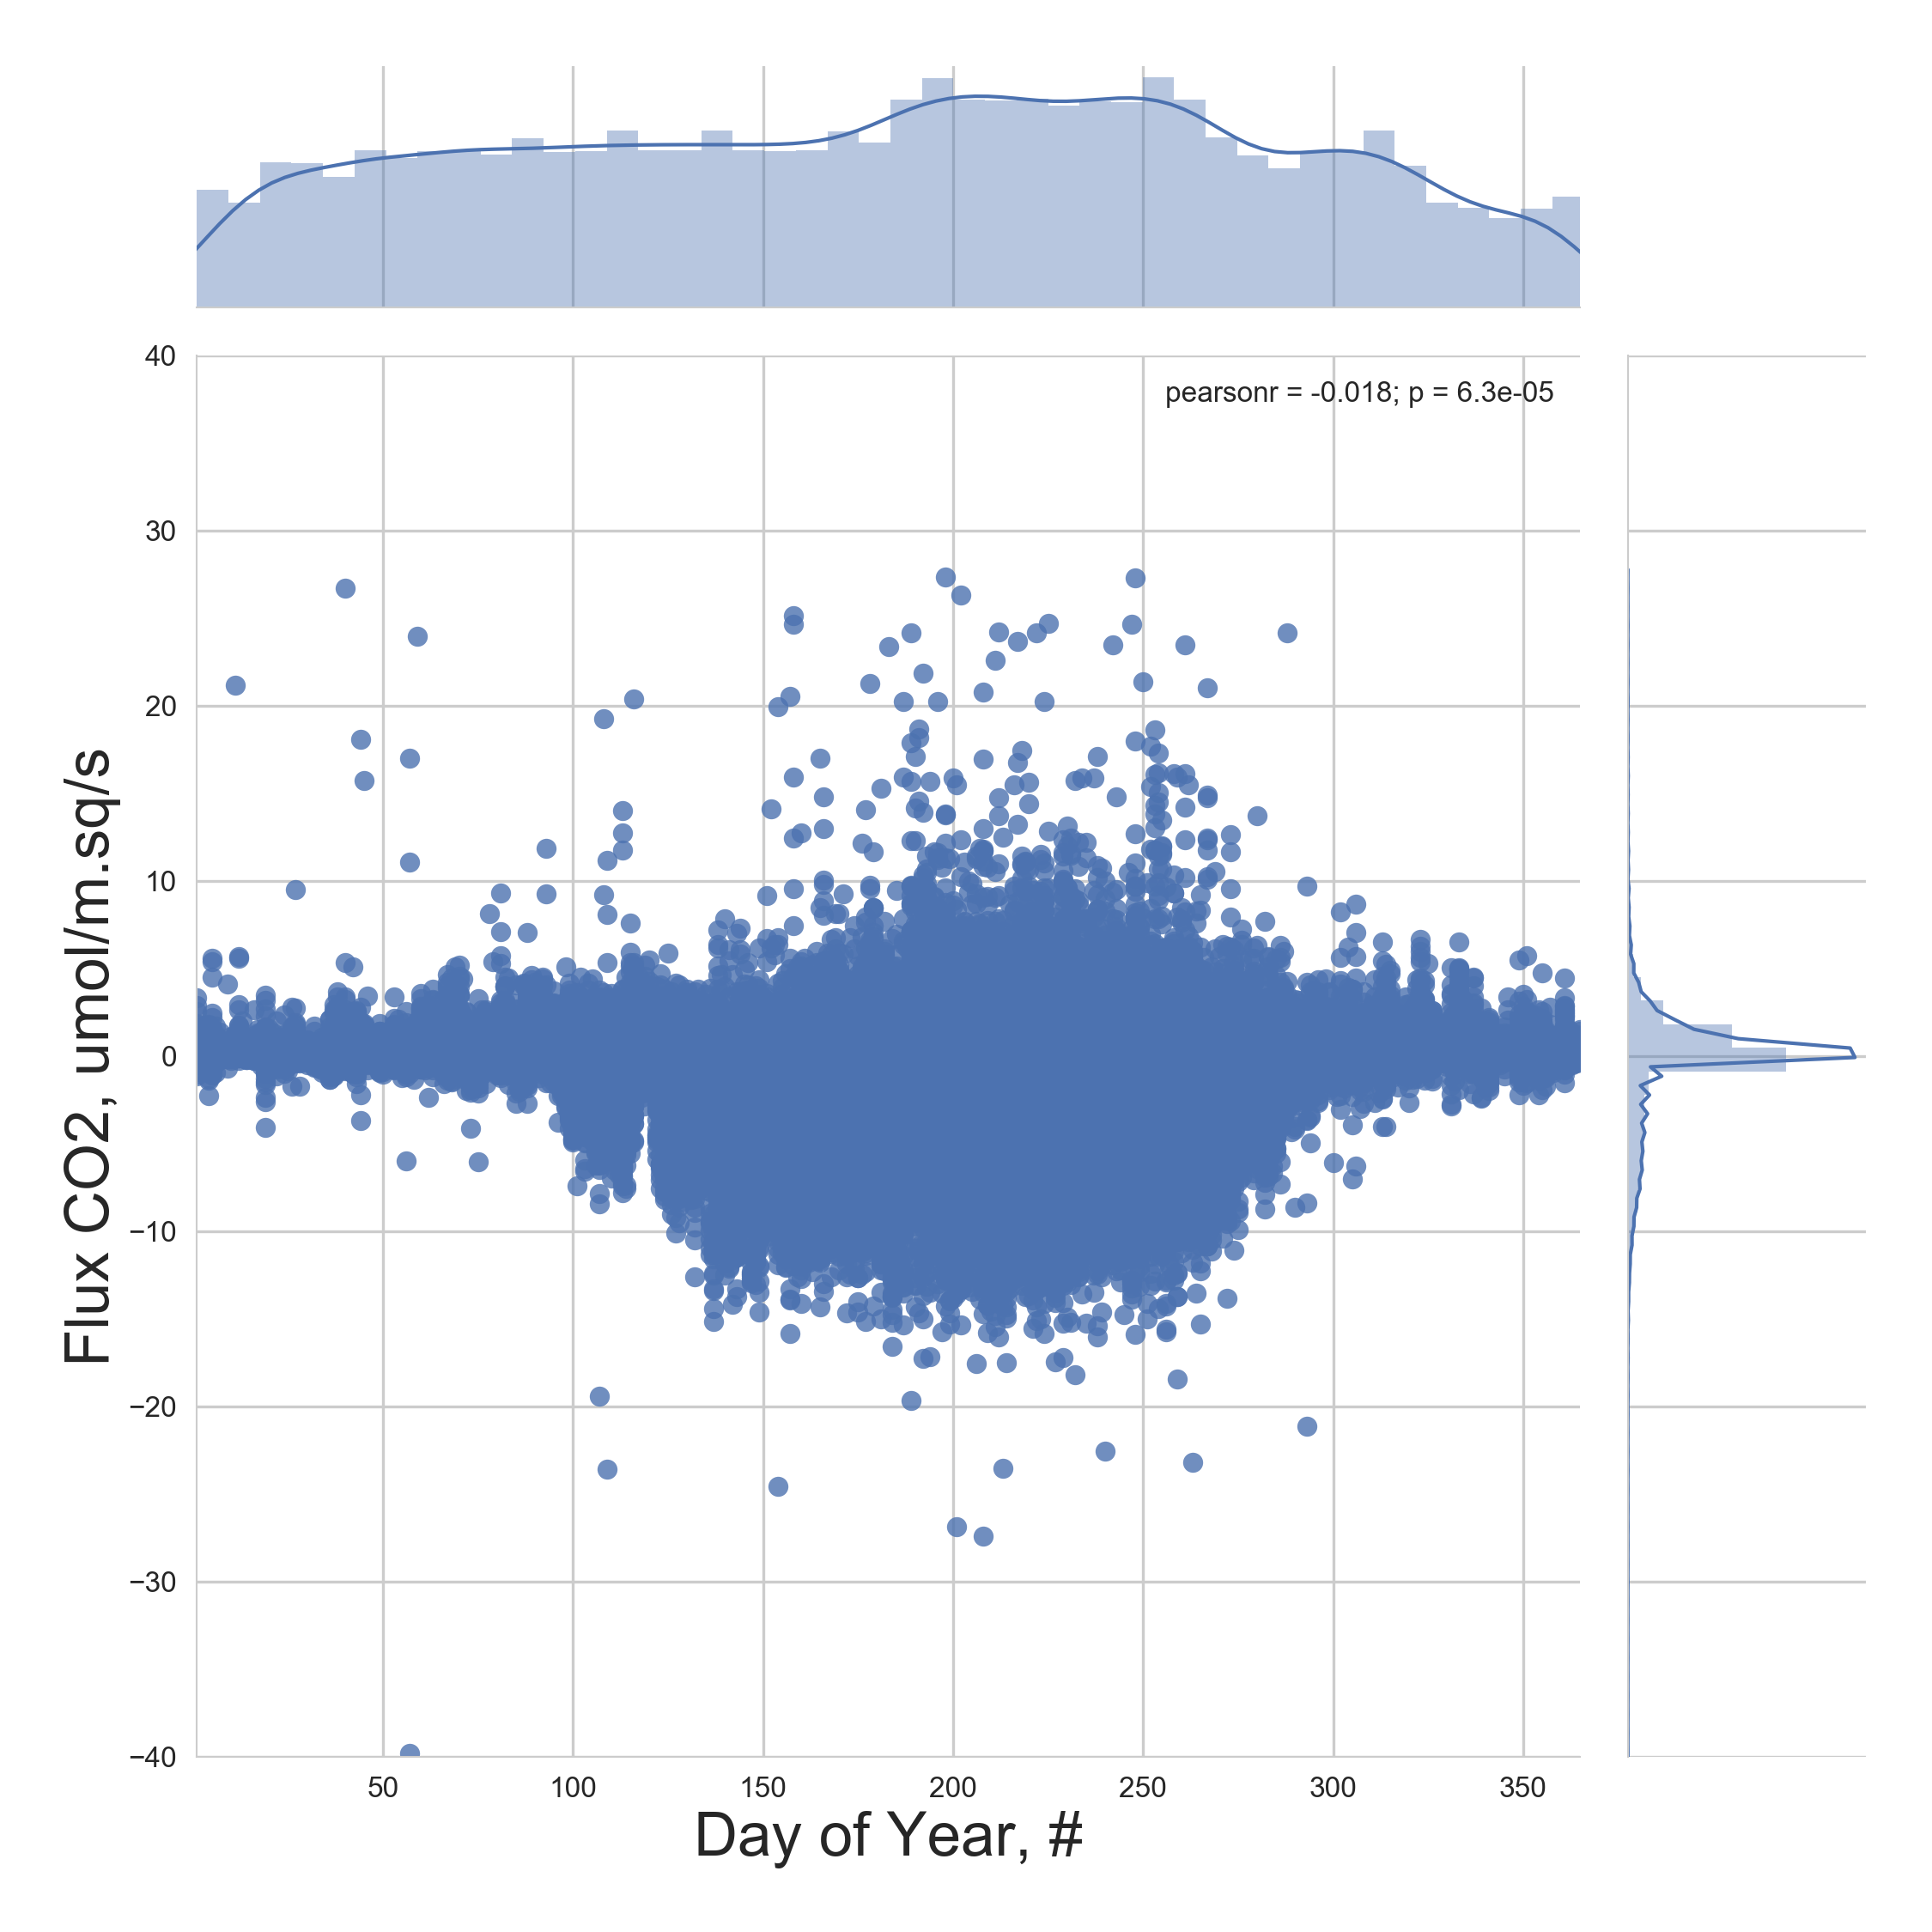
\includegraphics[width=\textwidth]{FvsY/CA-NS1.png}
\column{.35\textwidth}
\centering
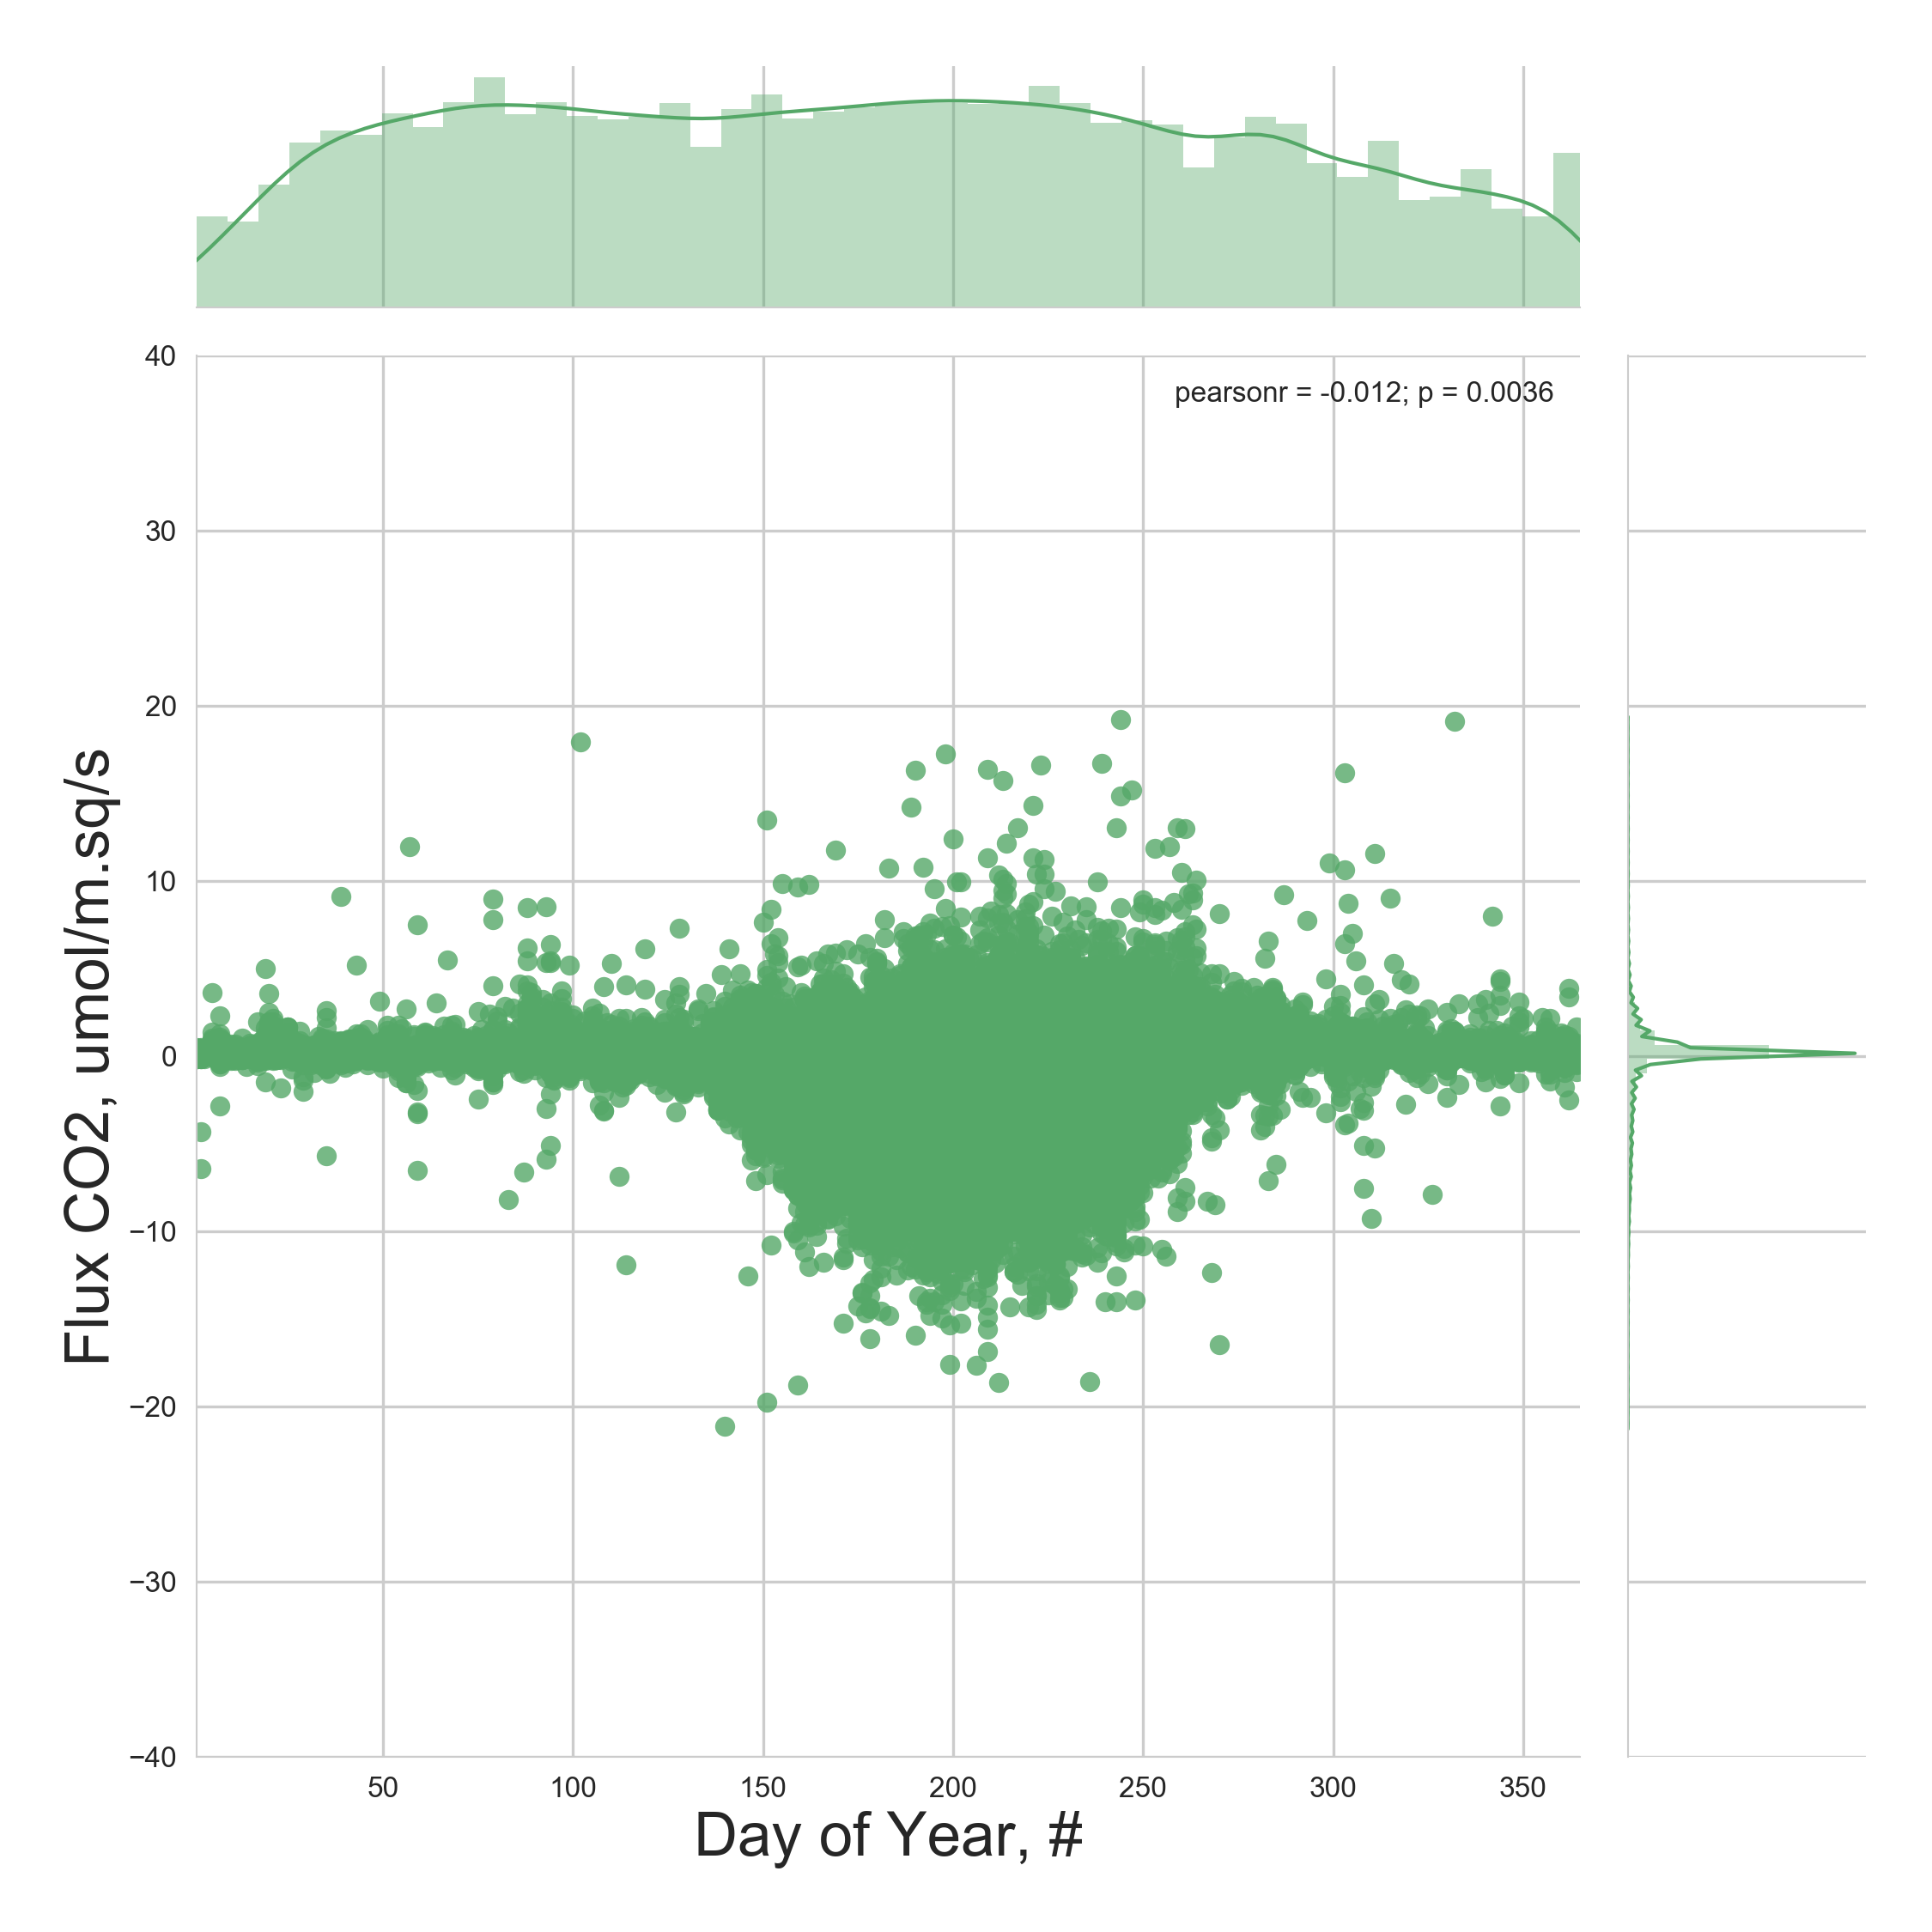
\includegraphics[width=\textwidth]{FvsY/CA-NS6.png}\\
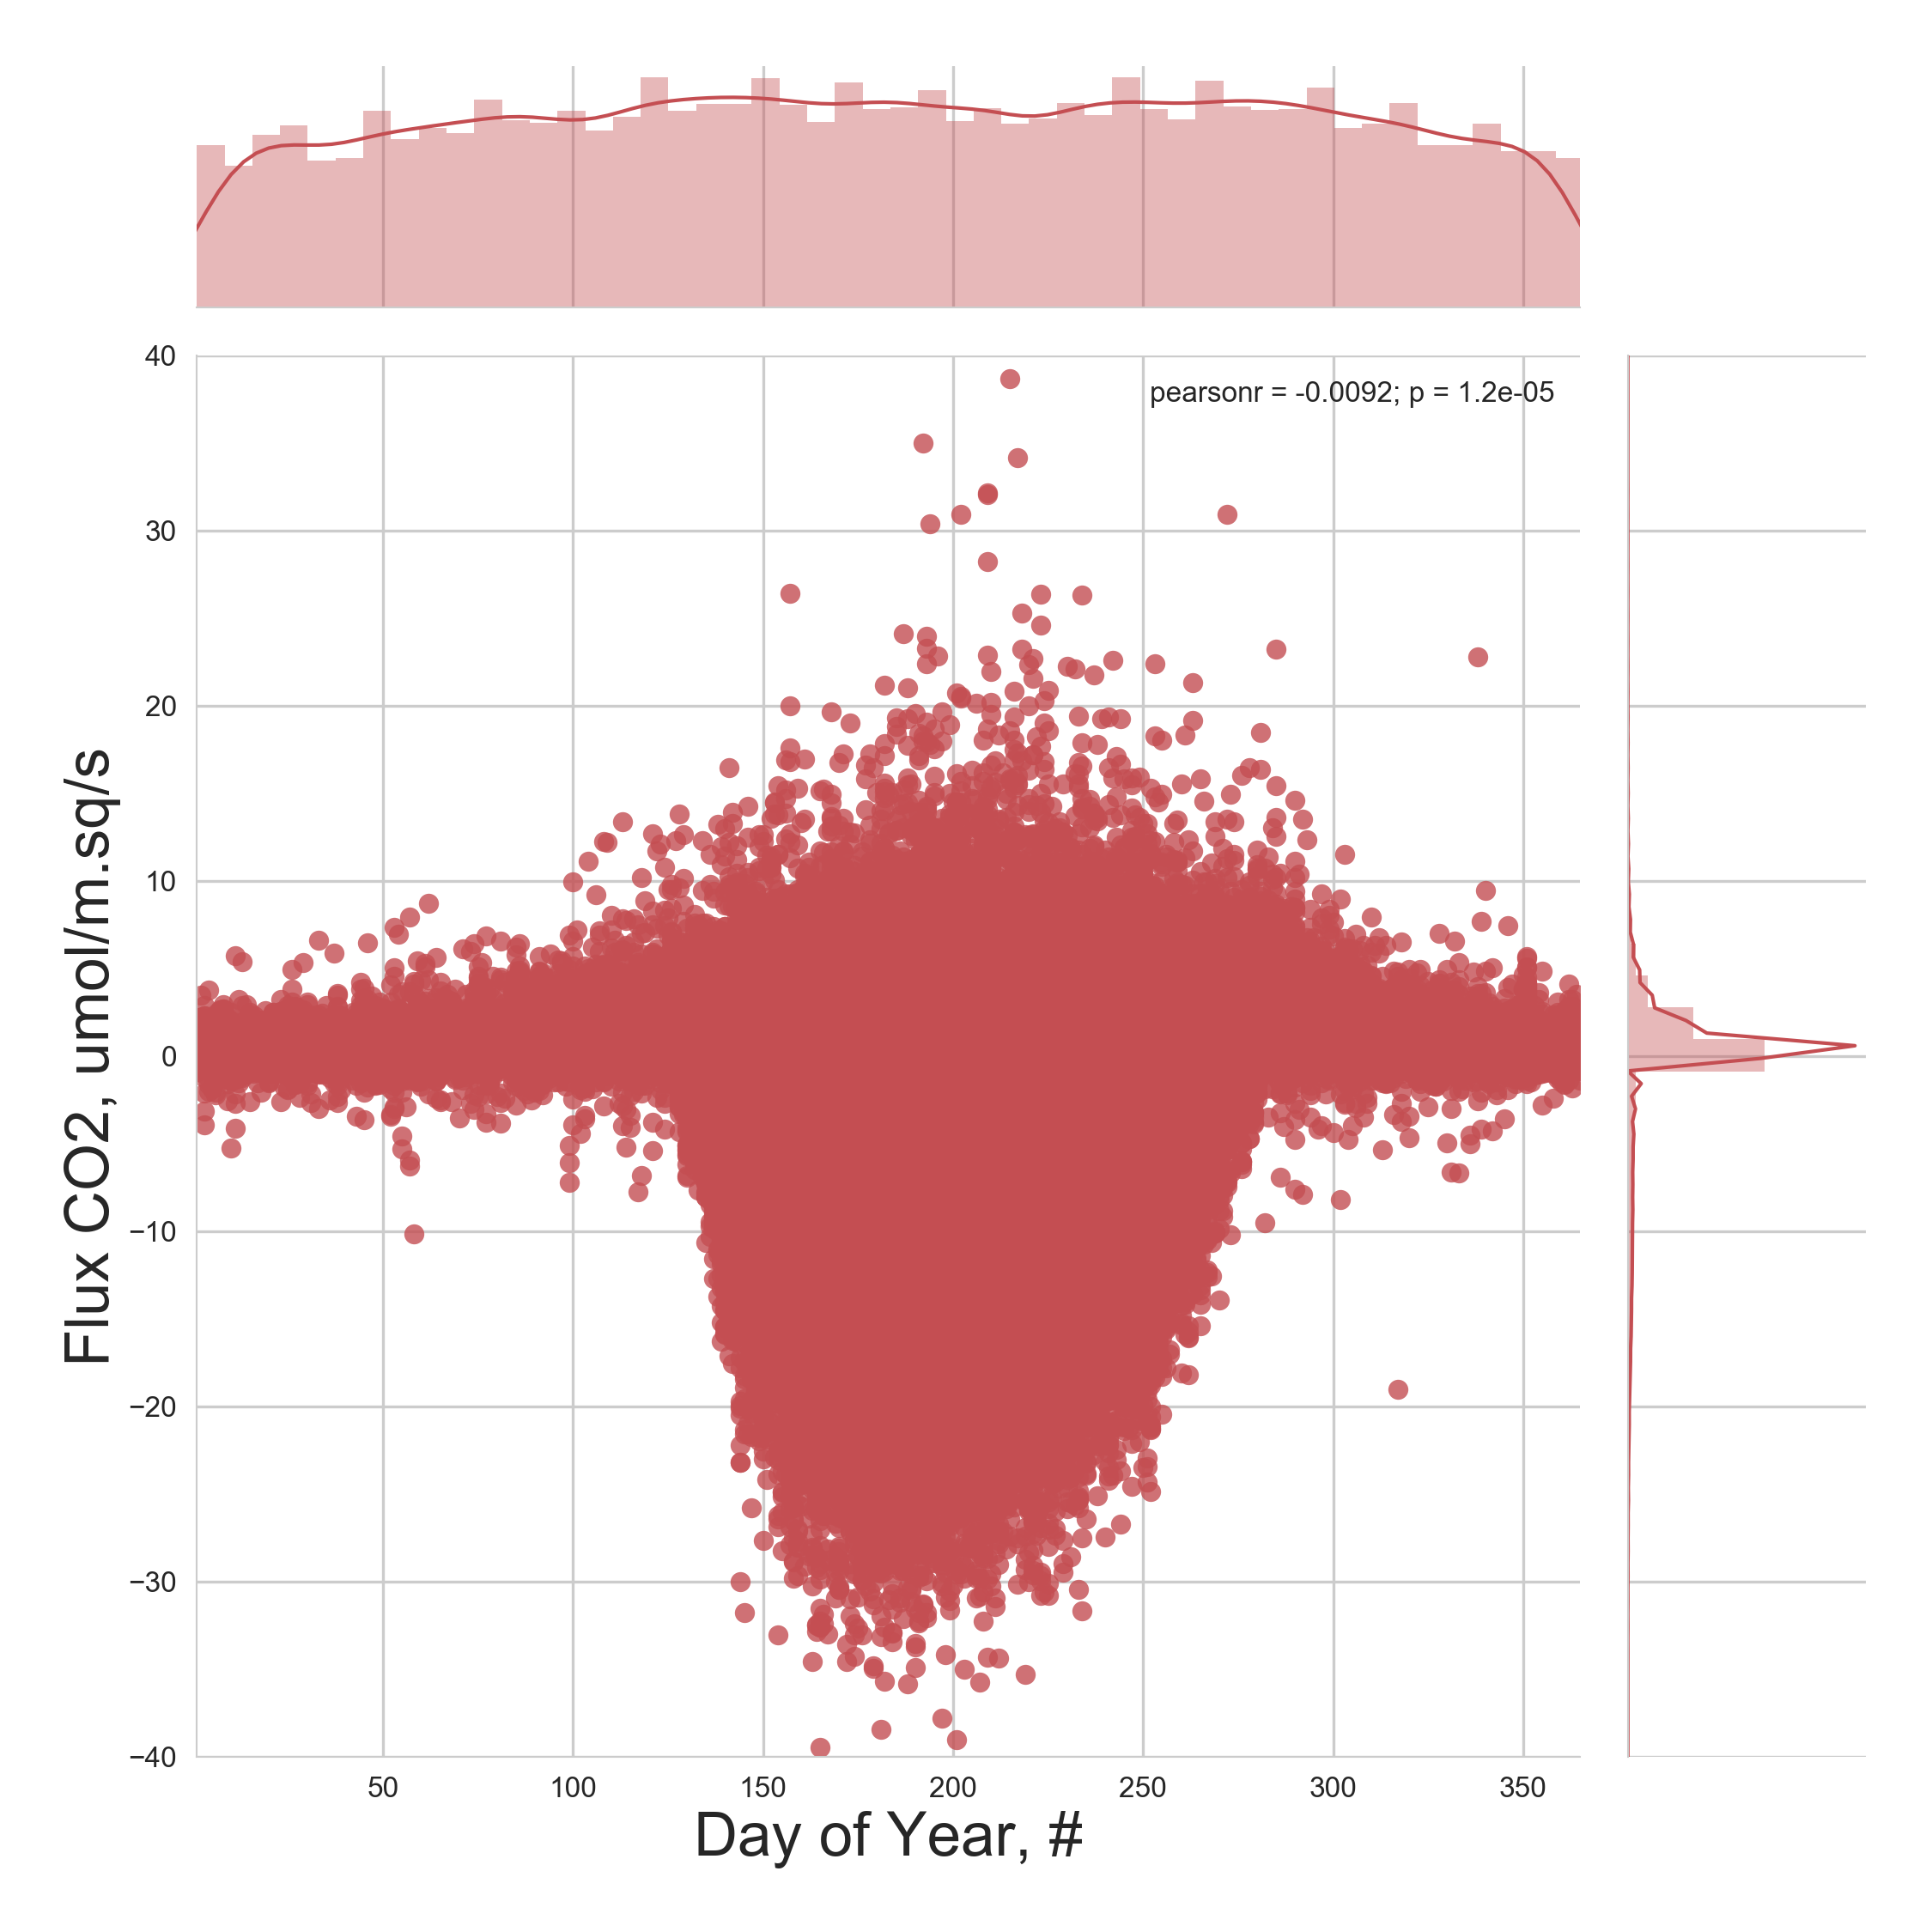
\includegraphics[width=\textwidth]{FvsY/CA-Oas.png}
\column{.35\textwidth}
\centering
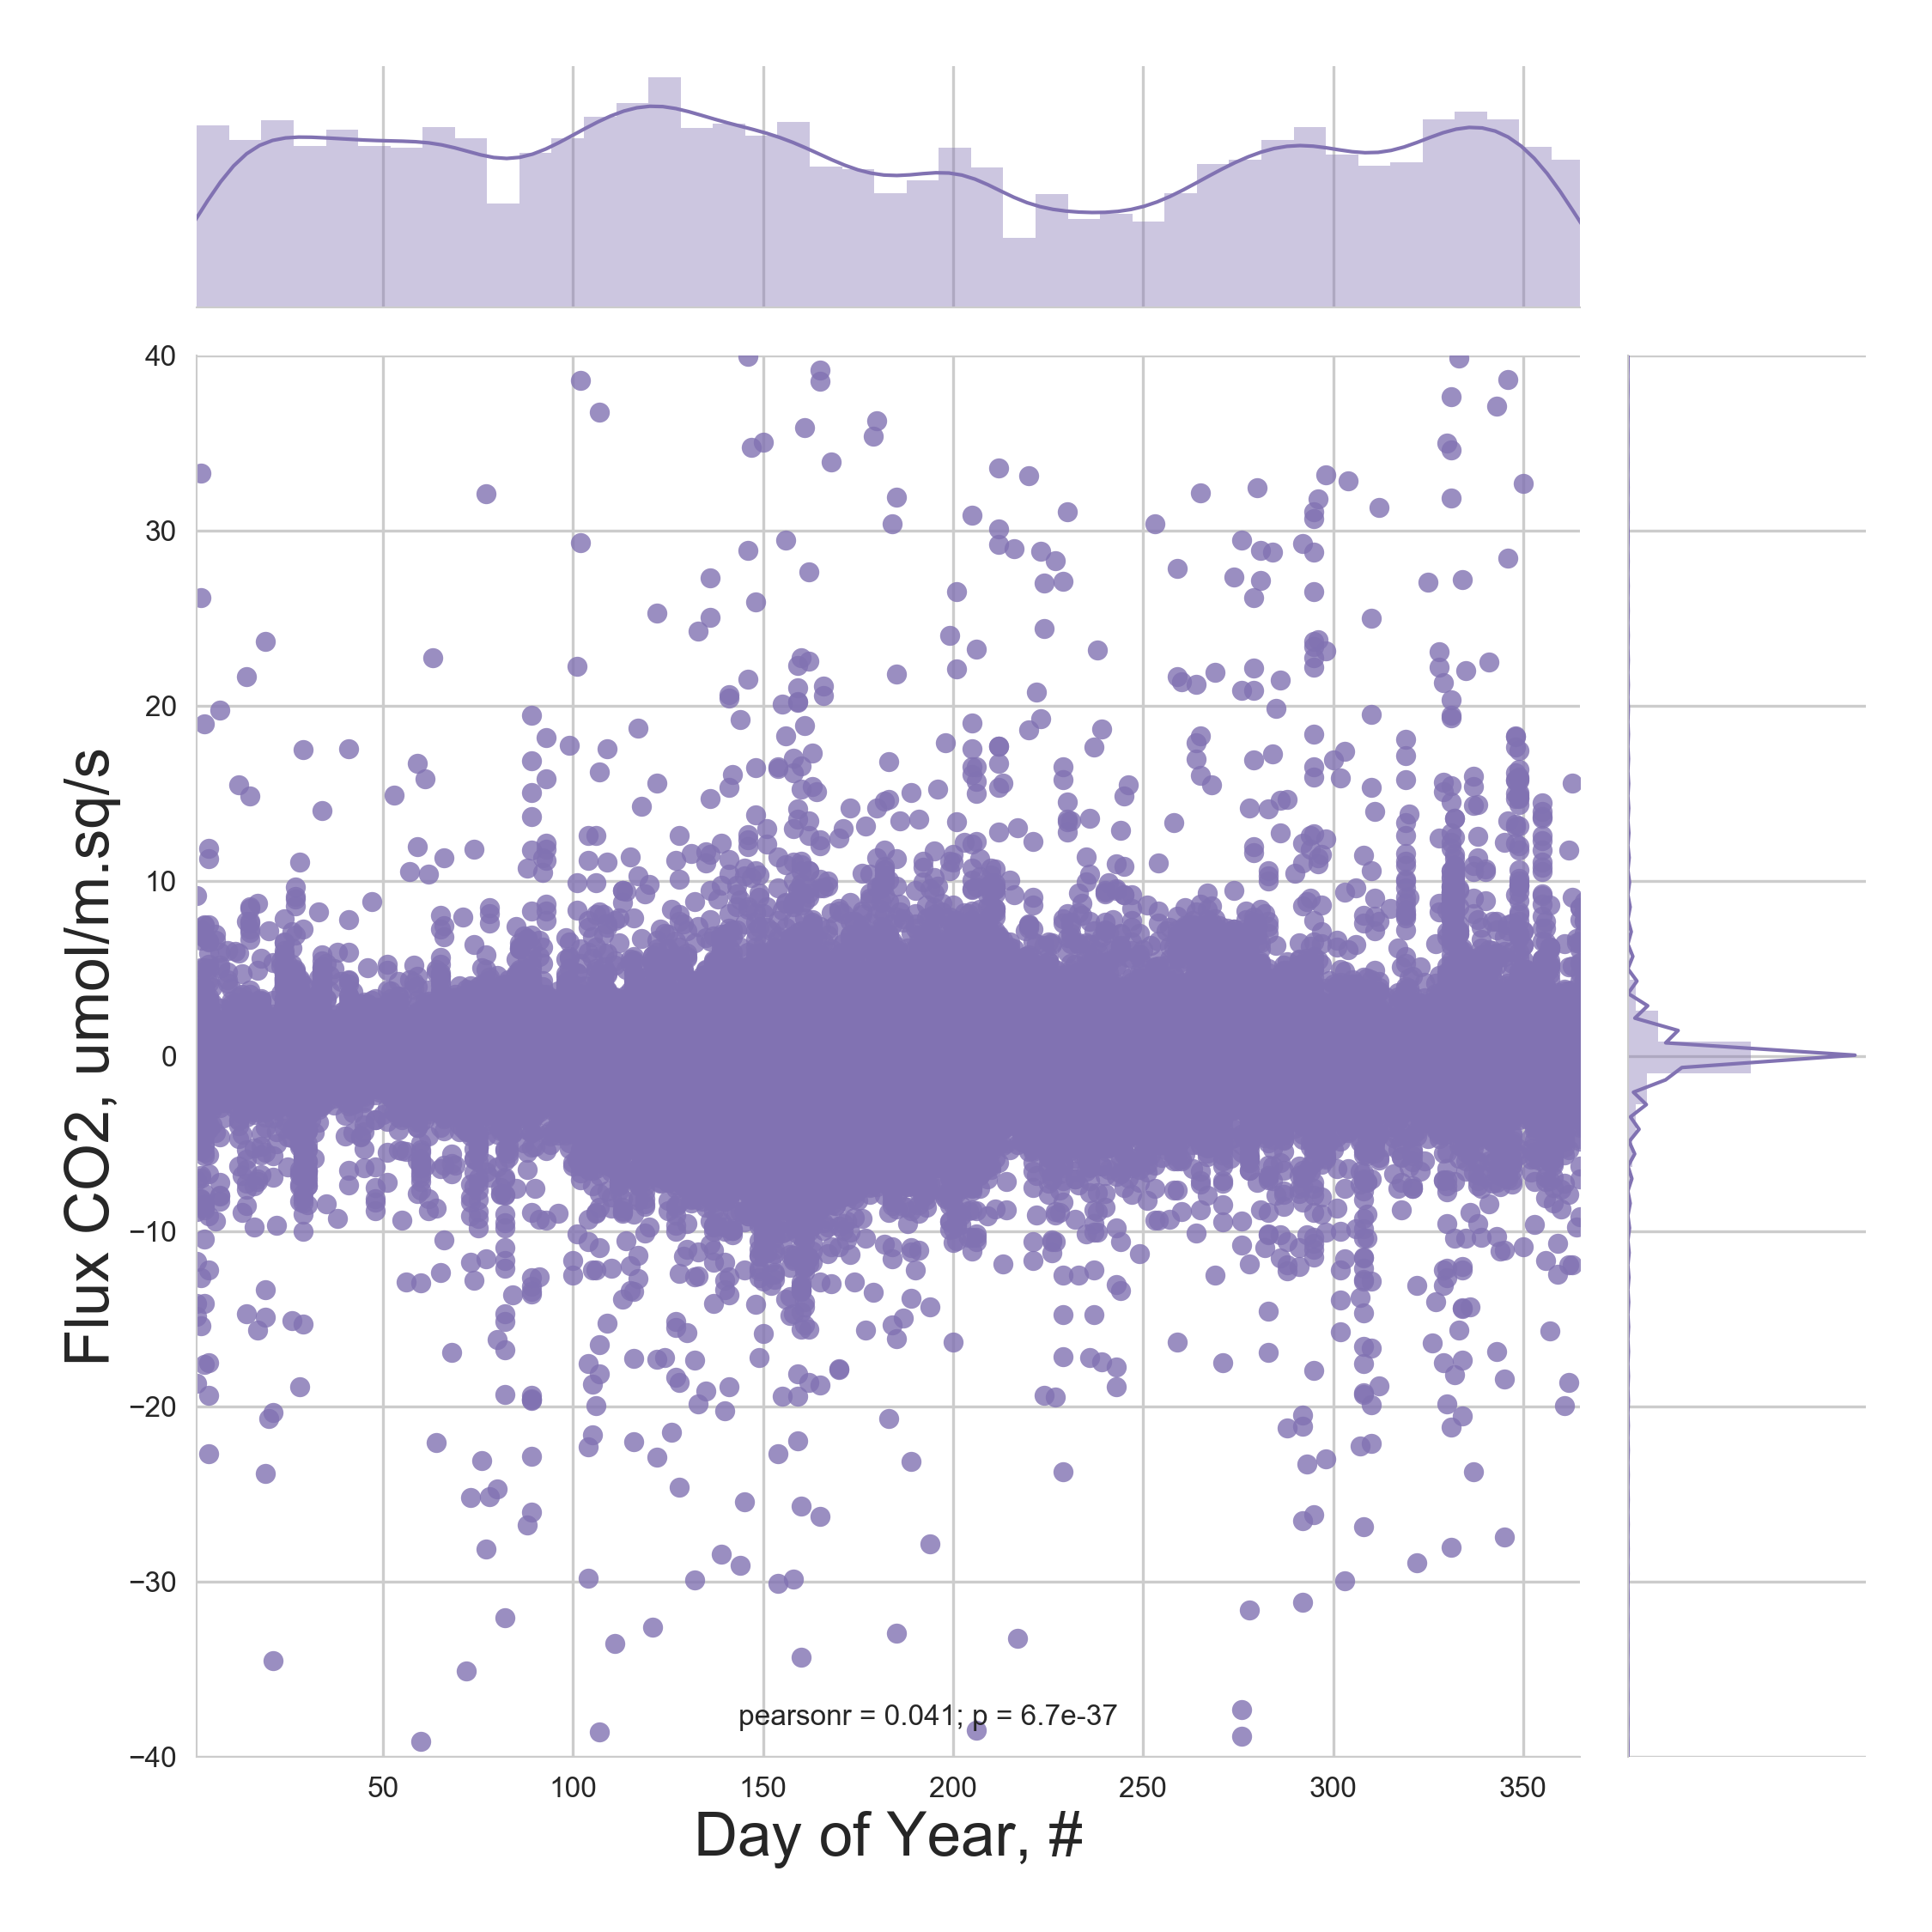
\includegraphics[width=\textwidth]{FvsY/US-FPe.png}\\
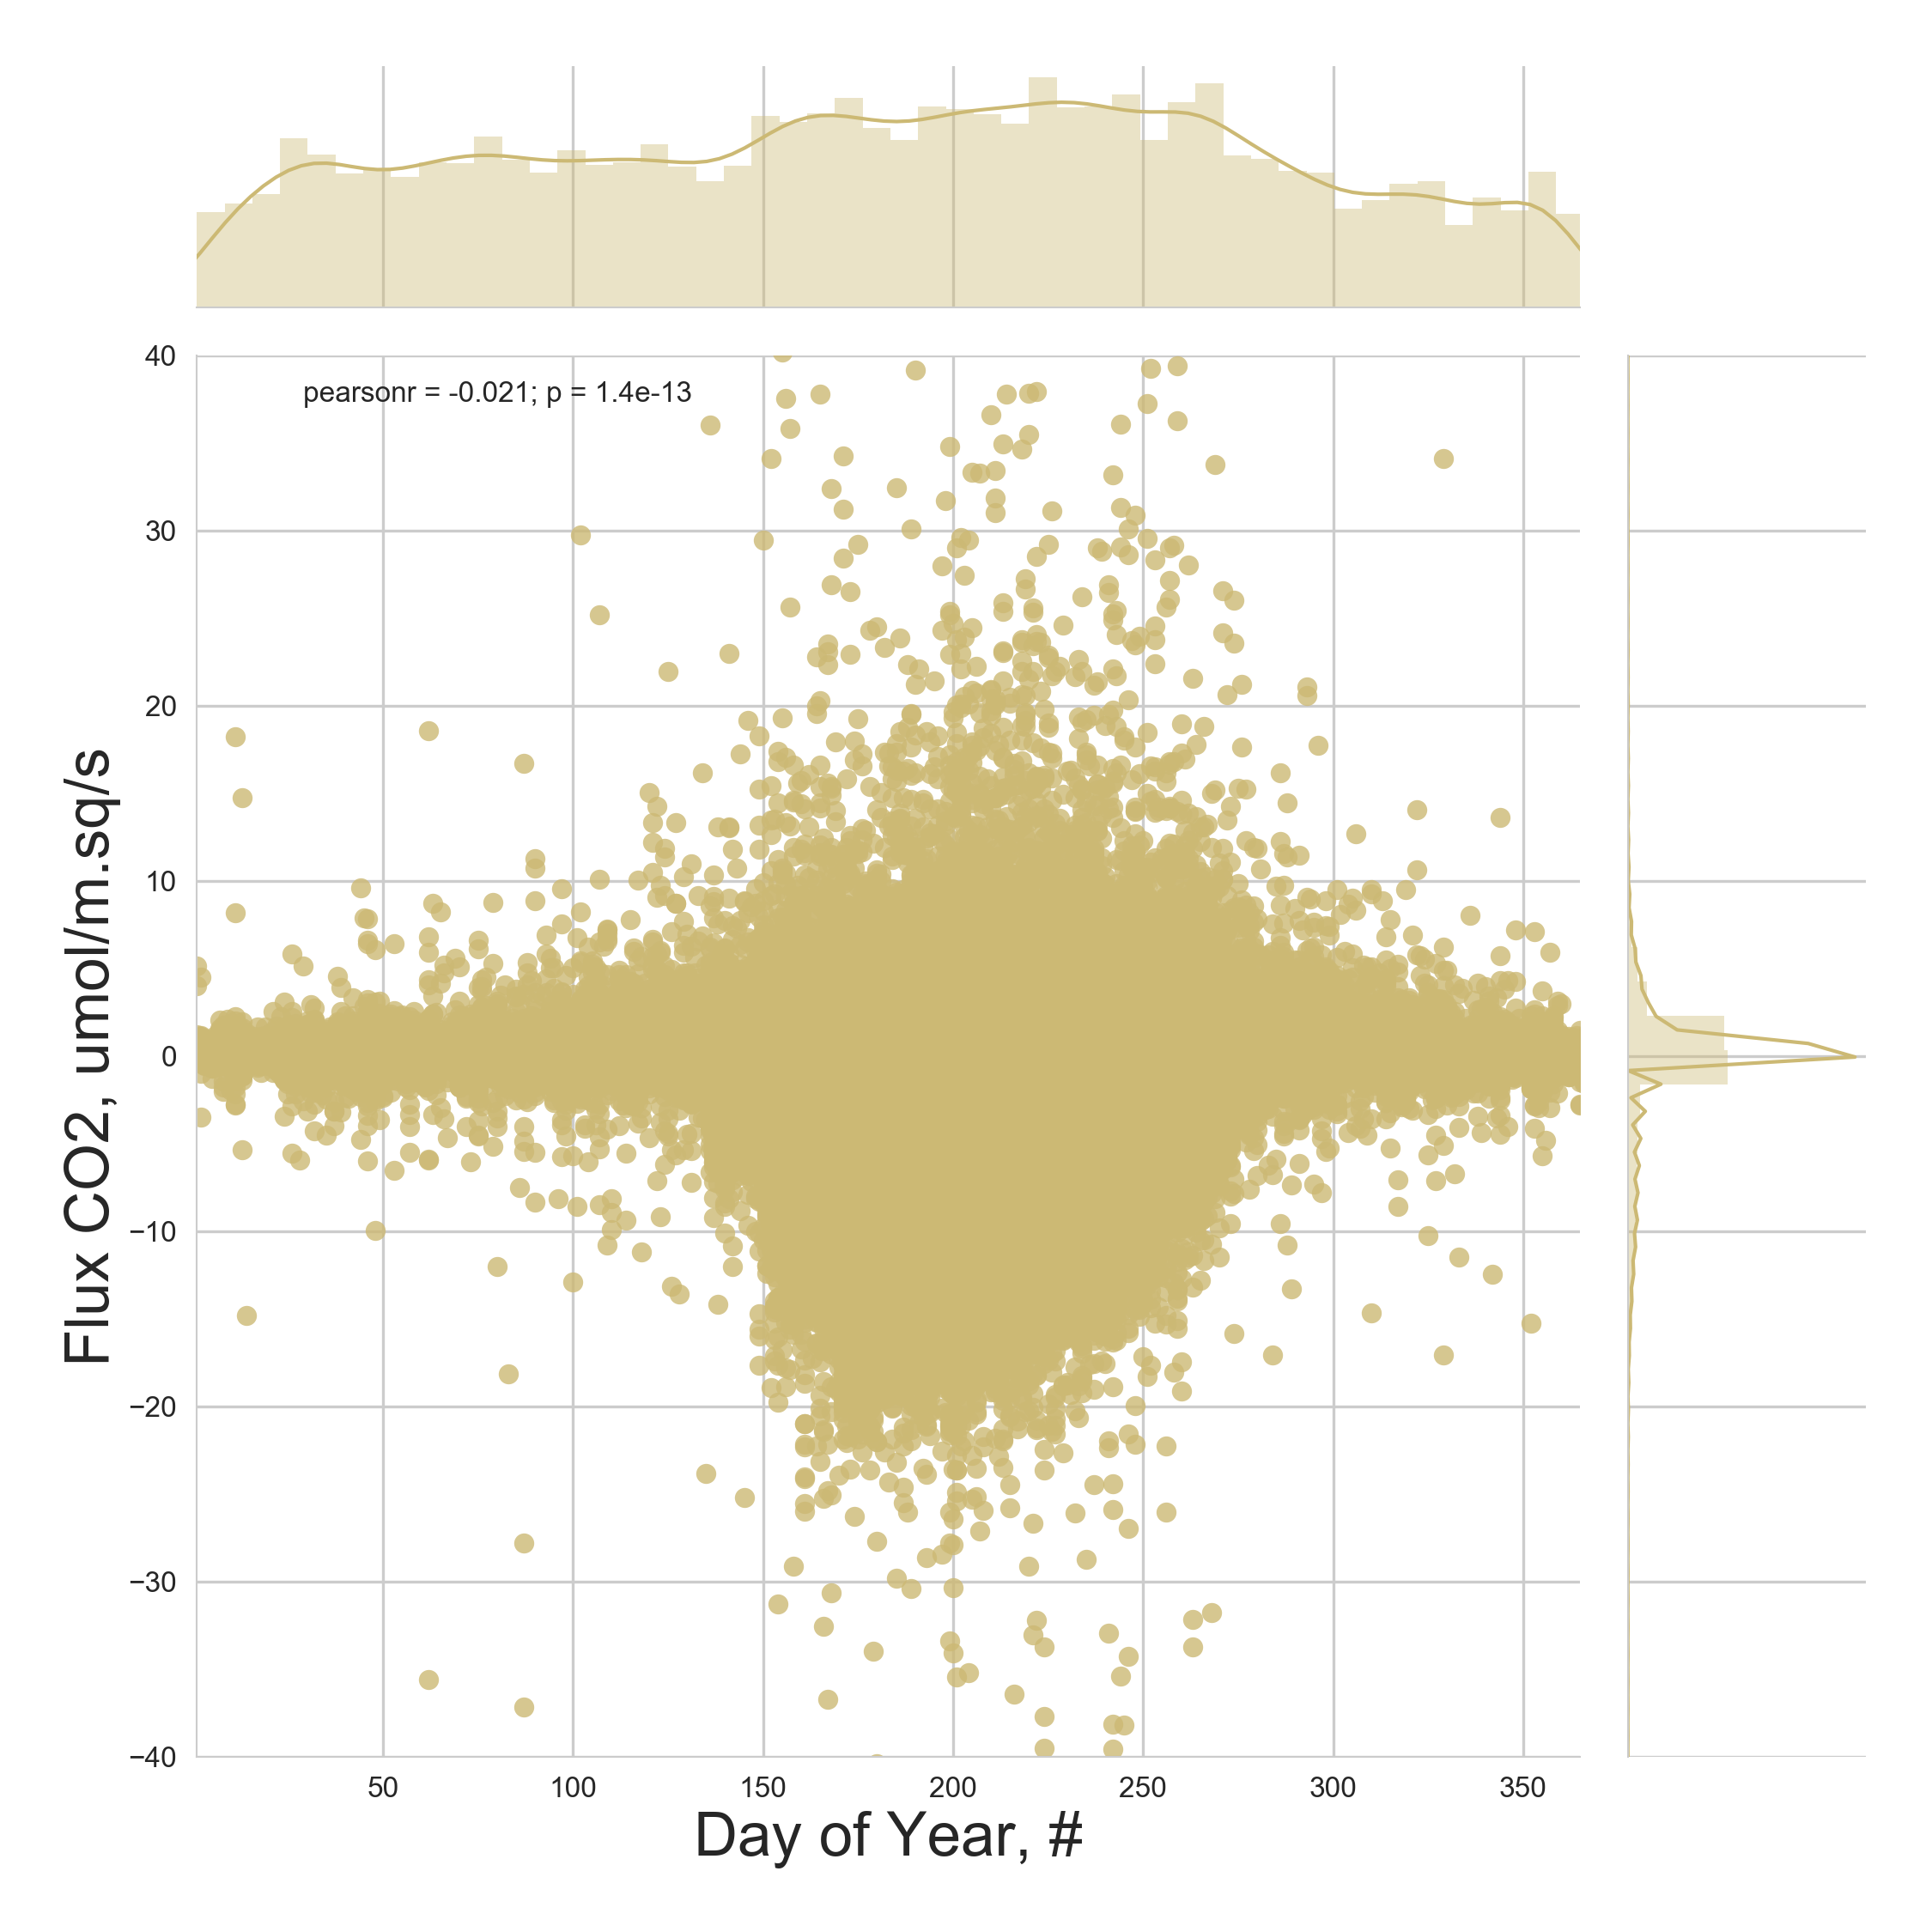
\includegraphics[width=\textwidth]{FvsY/US-Los.png}
\end{columns}

\end{frame}

% \begin{frame}
% \frametitle{Weekly boxplots}

% \begin{columns}[t]
% \column{.35\textwidth}
% \centering
% 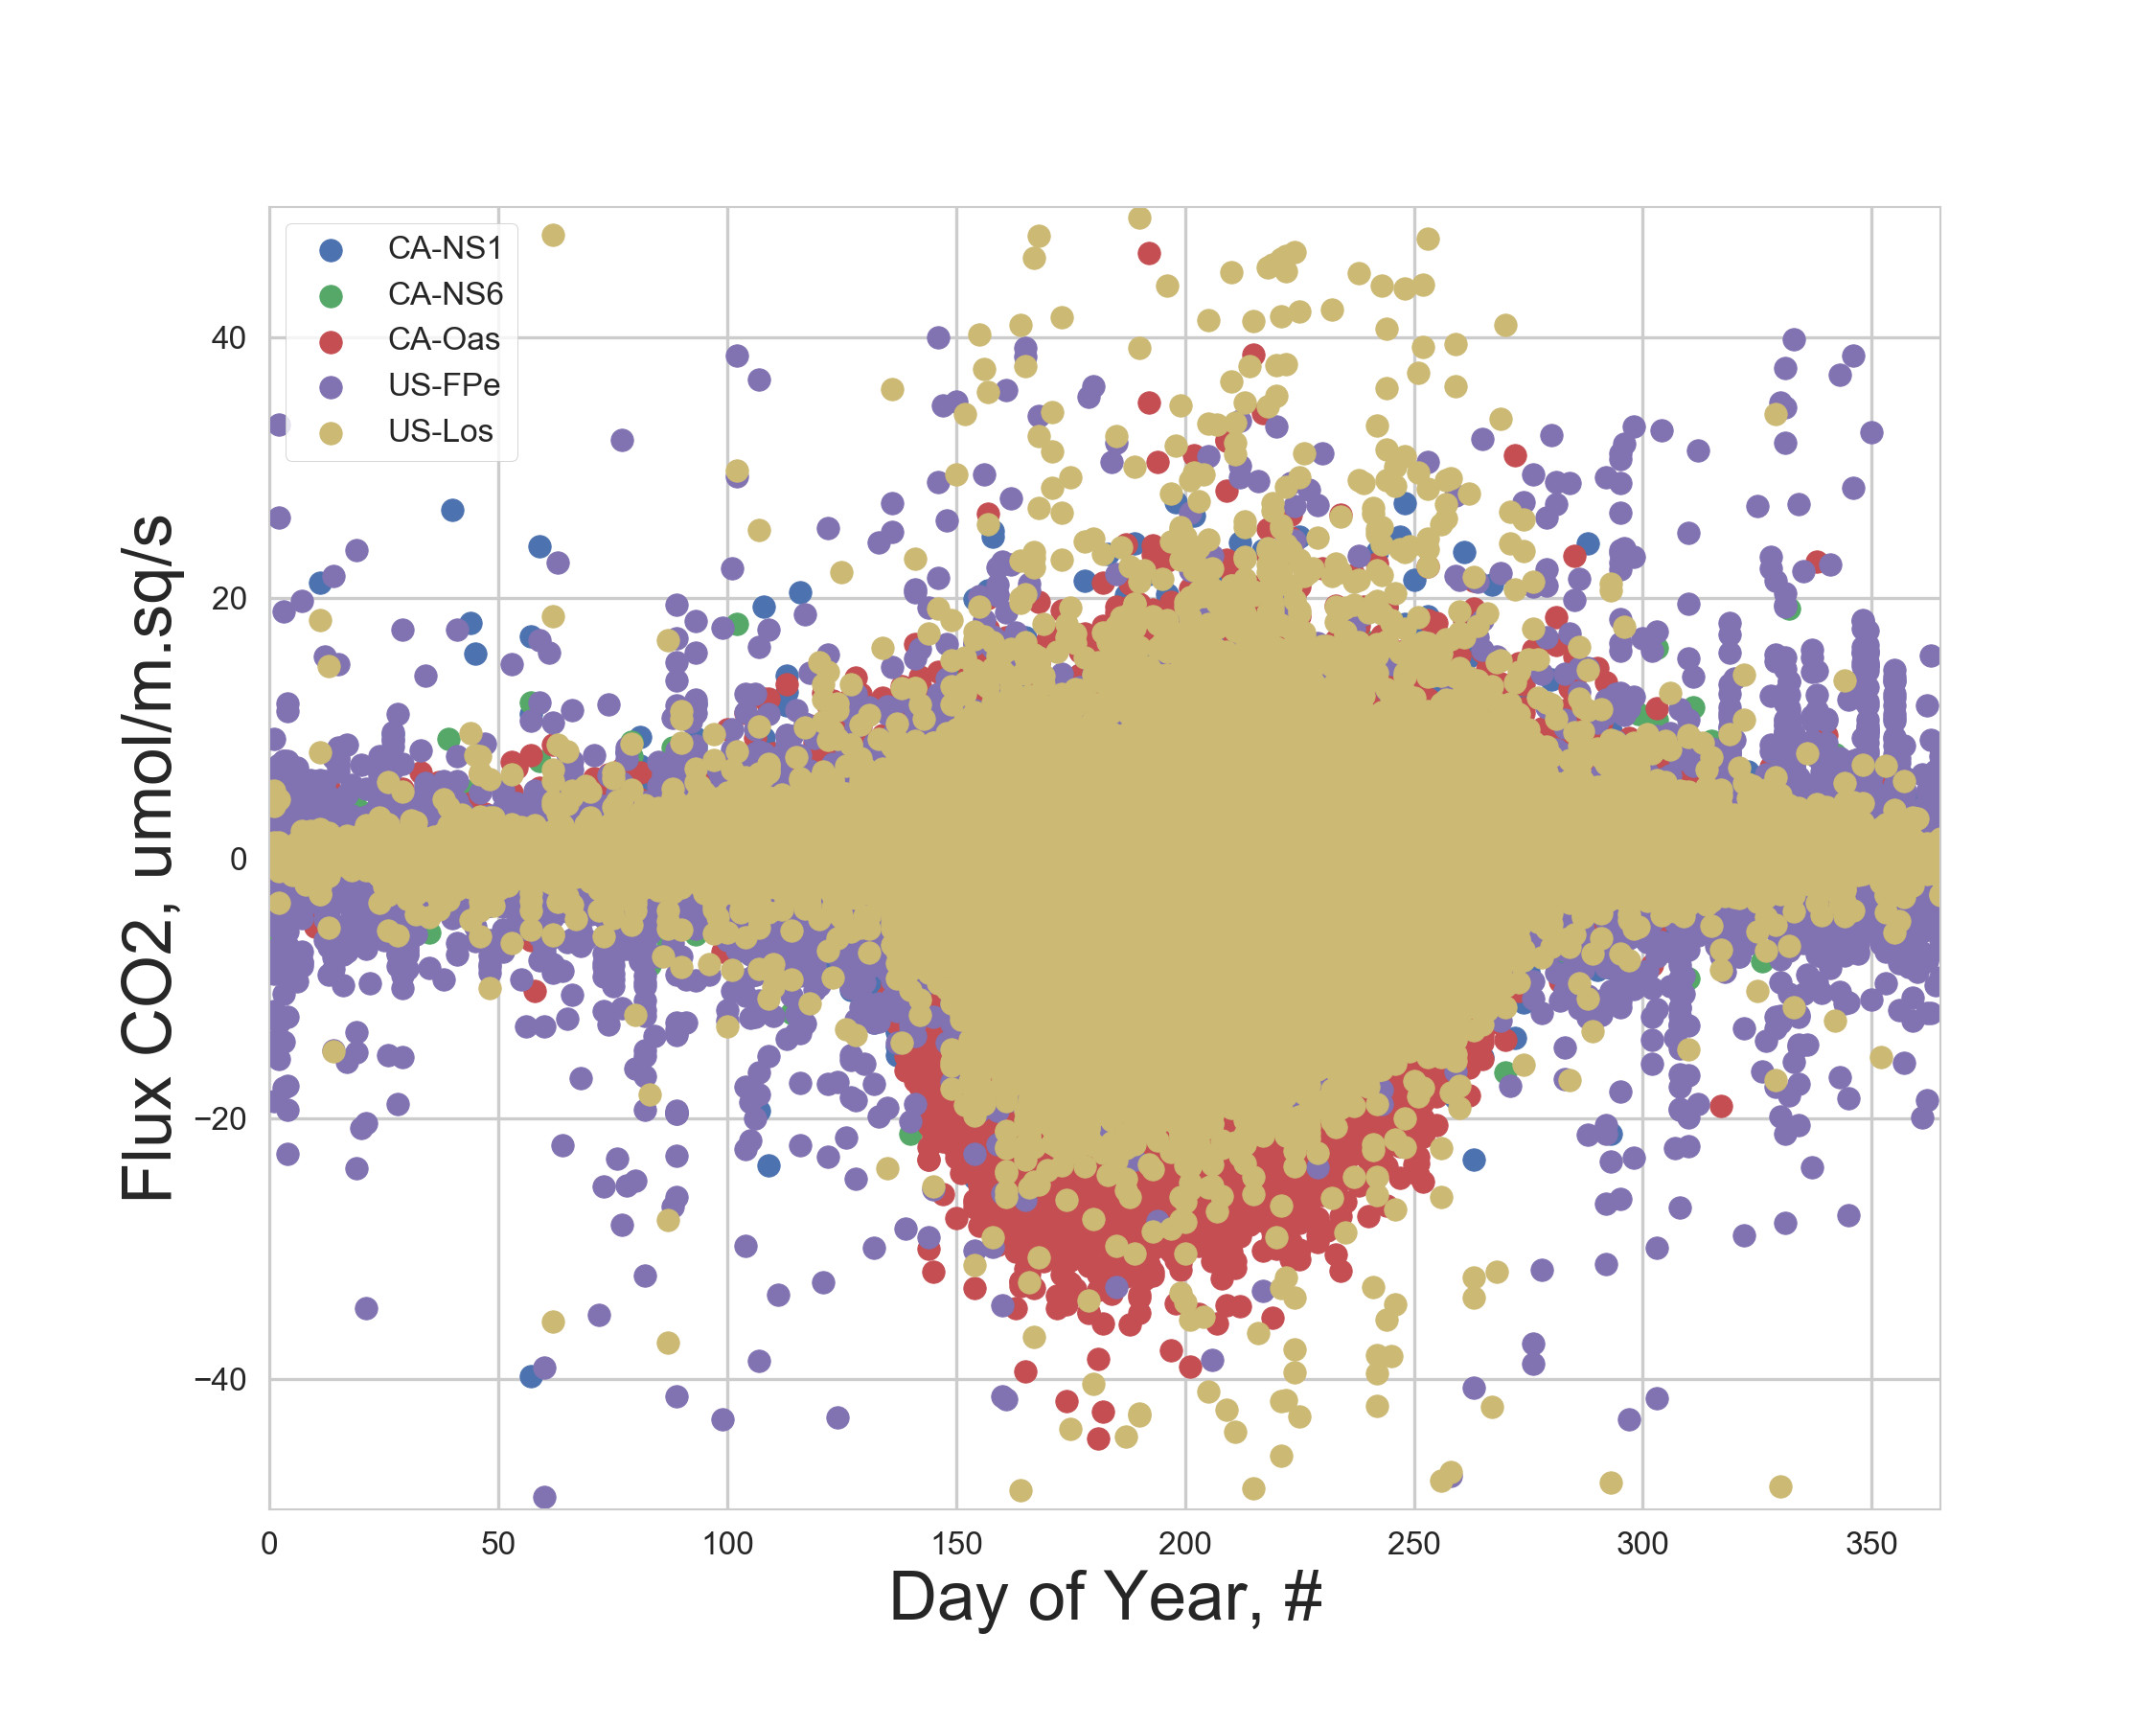
\includegraphics[width=\textwidth]{FvsY/all.png}\\
% 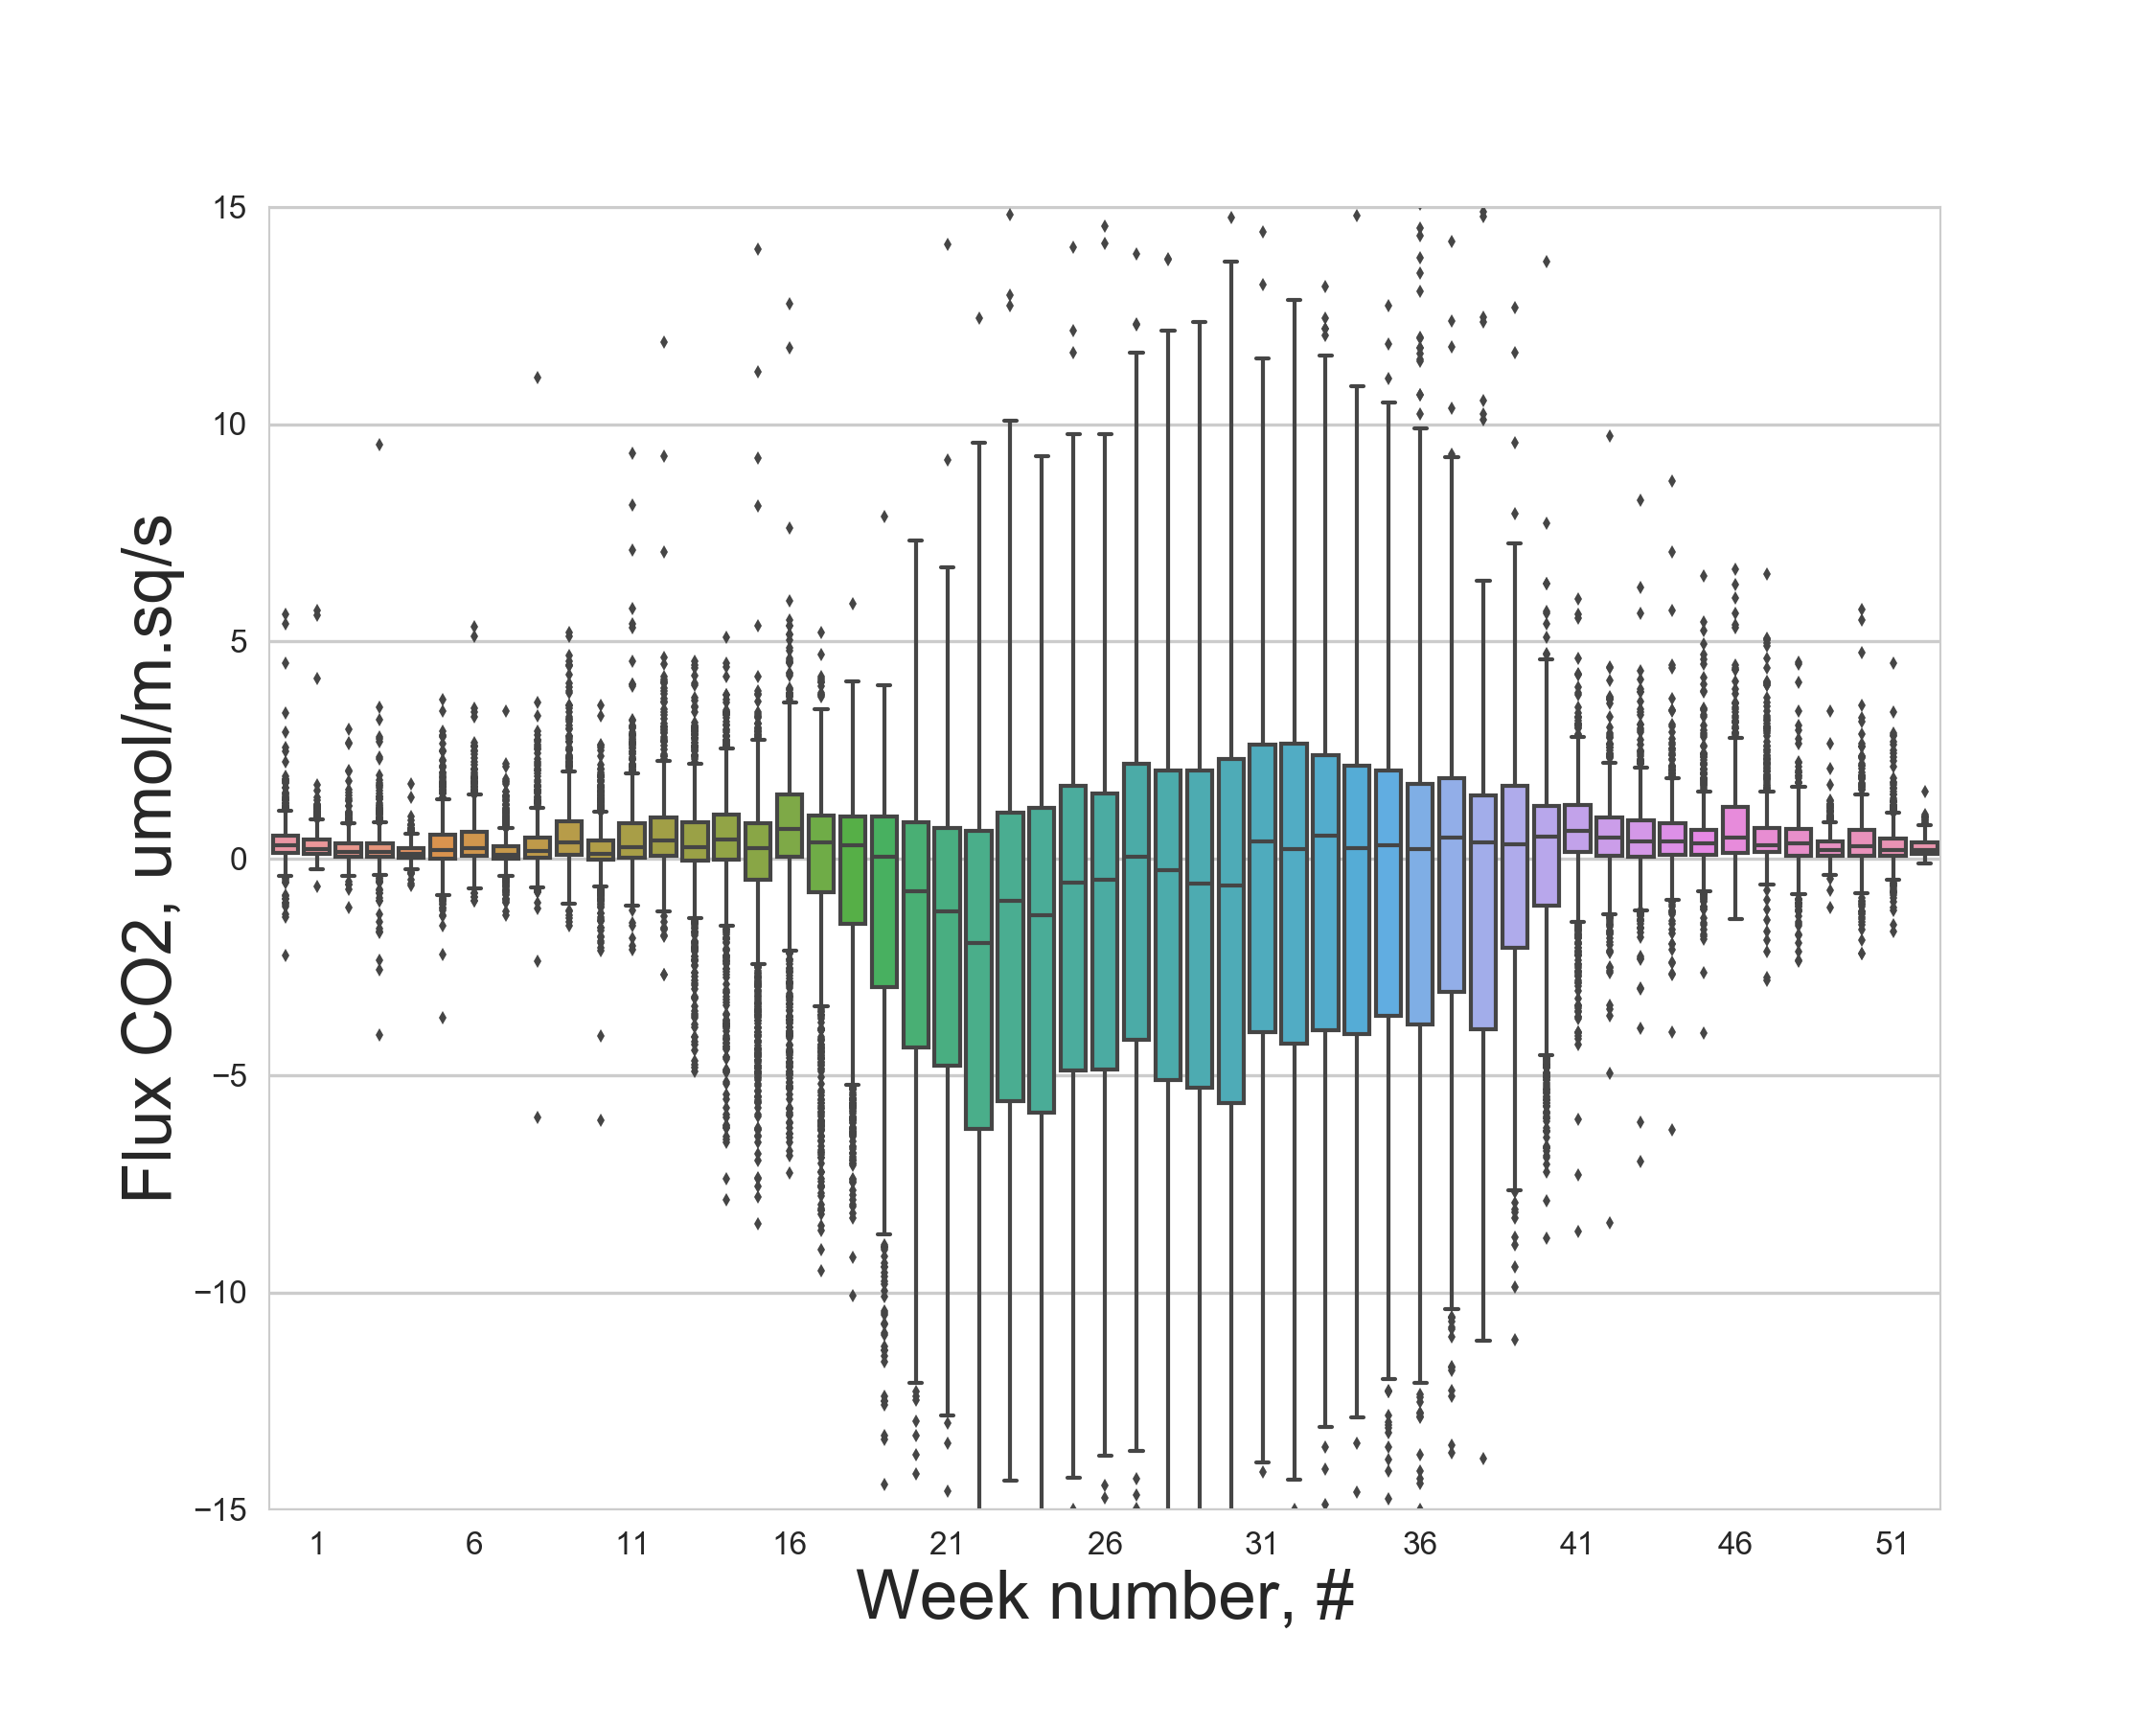
\includegraphics[width=\textwidth]{FvsW/CA-NS1.png}
% \column{.35\textwidth}
% \centering
% 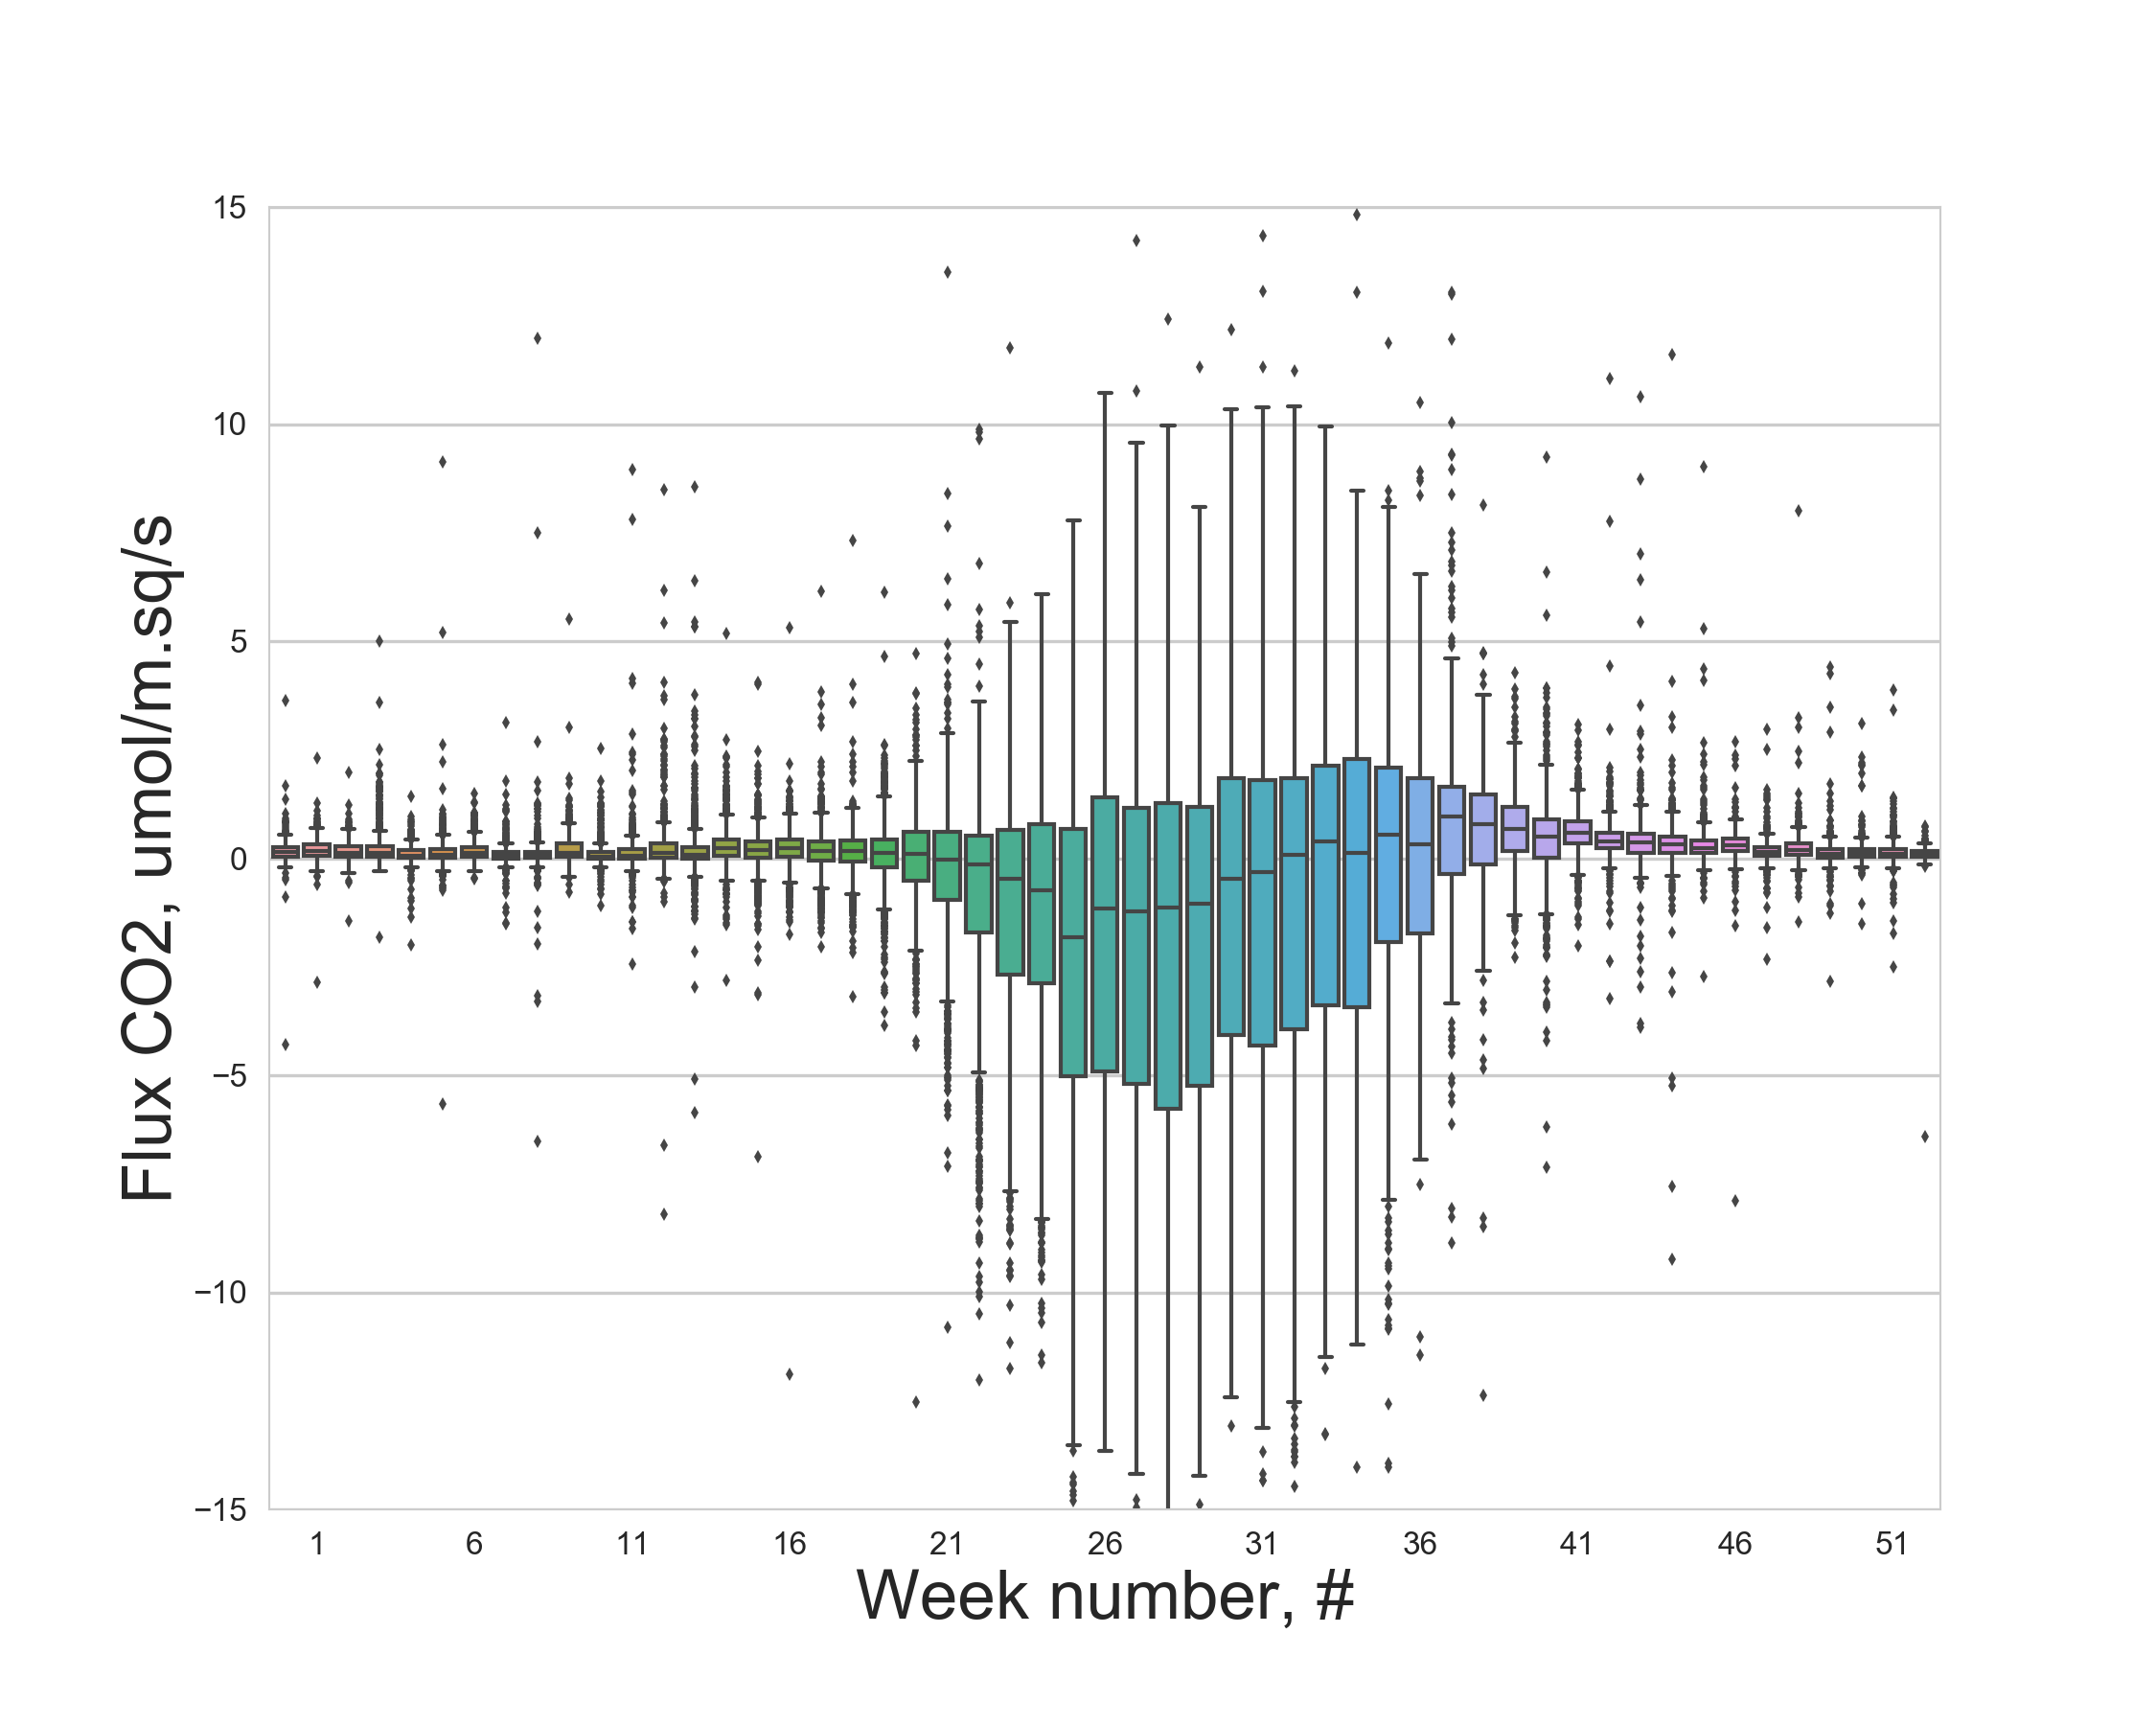
\includegraphics[width=\textwidth]{FvsW/CA-NS6.png}\\
% 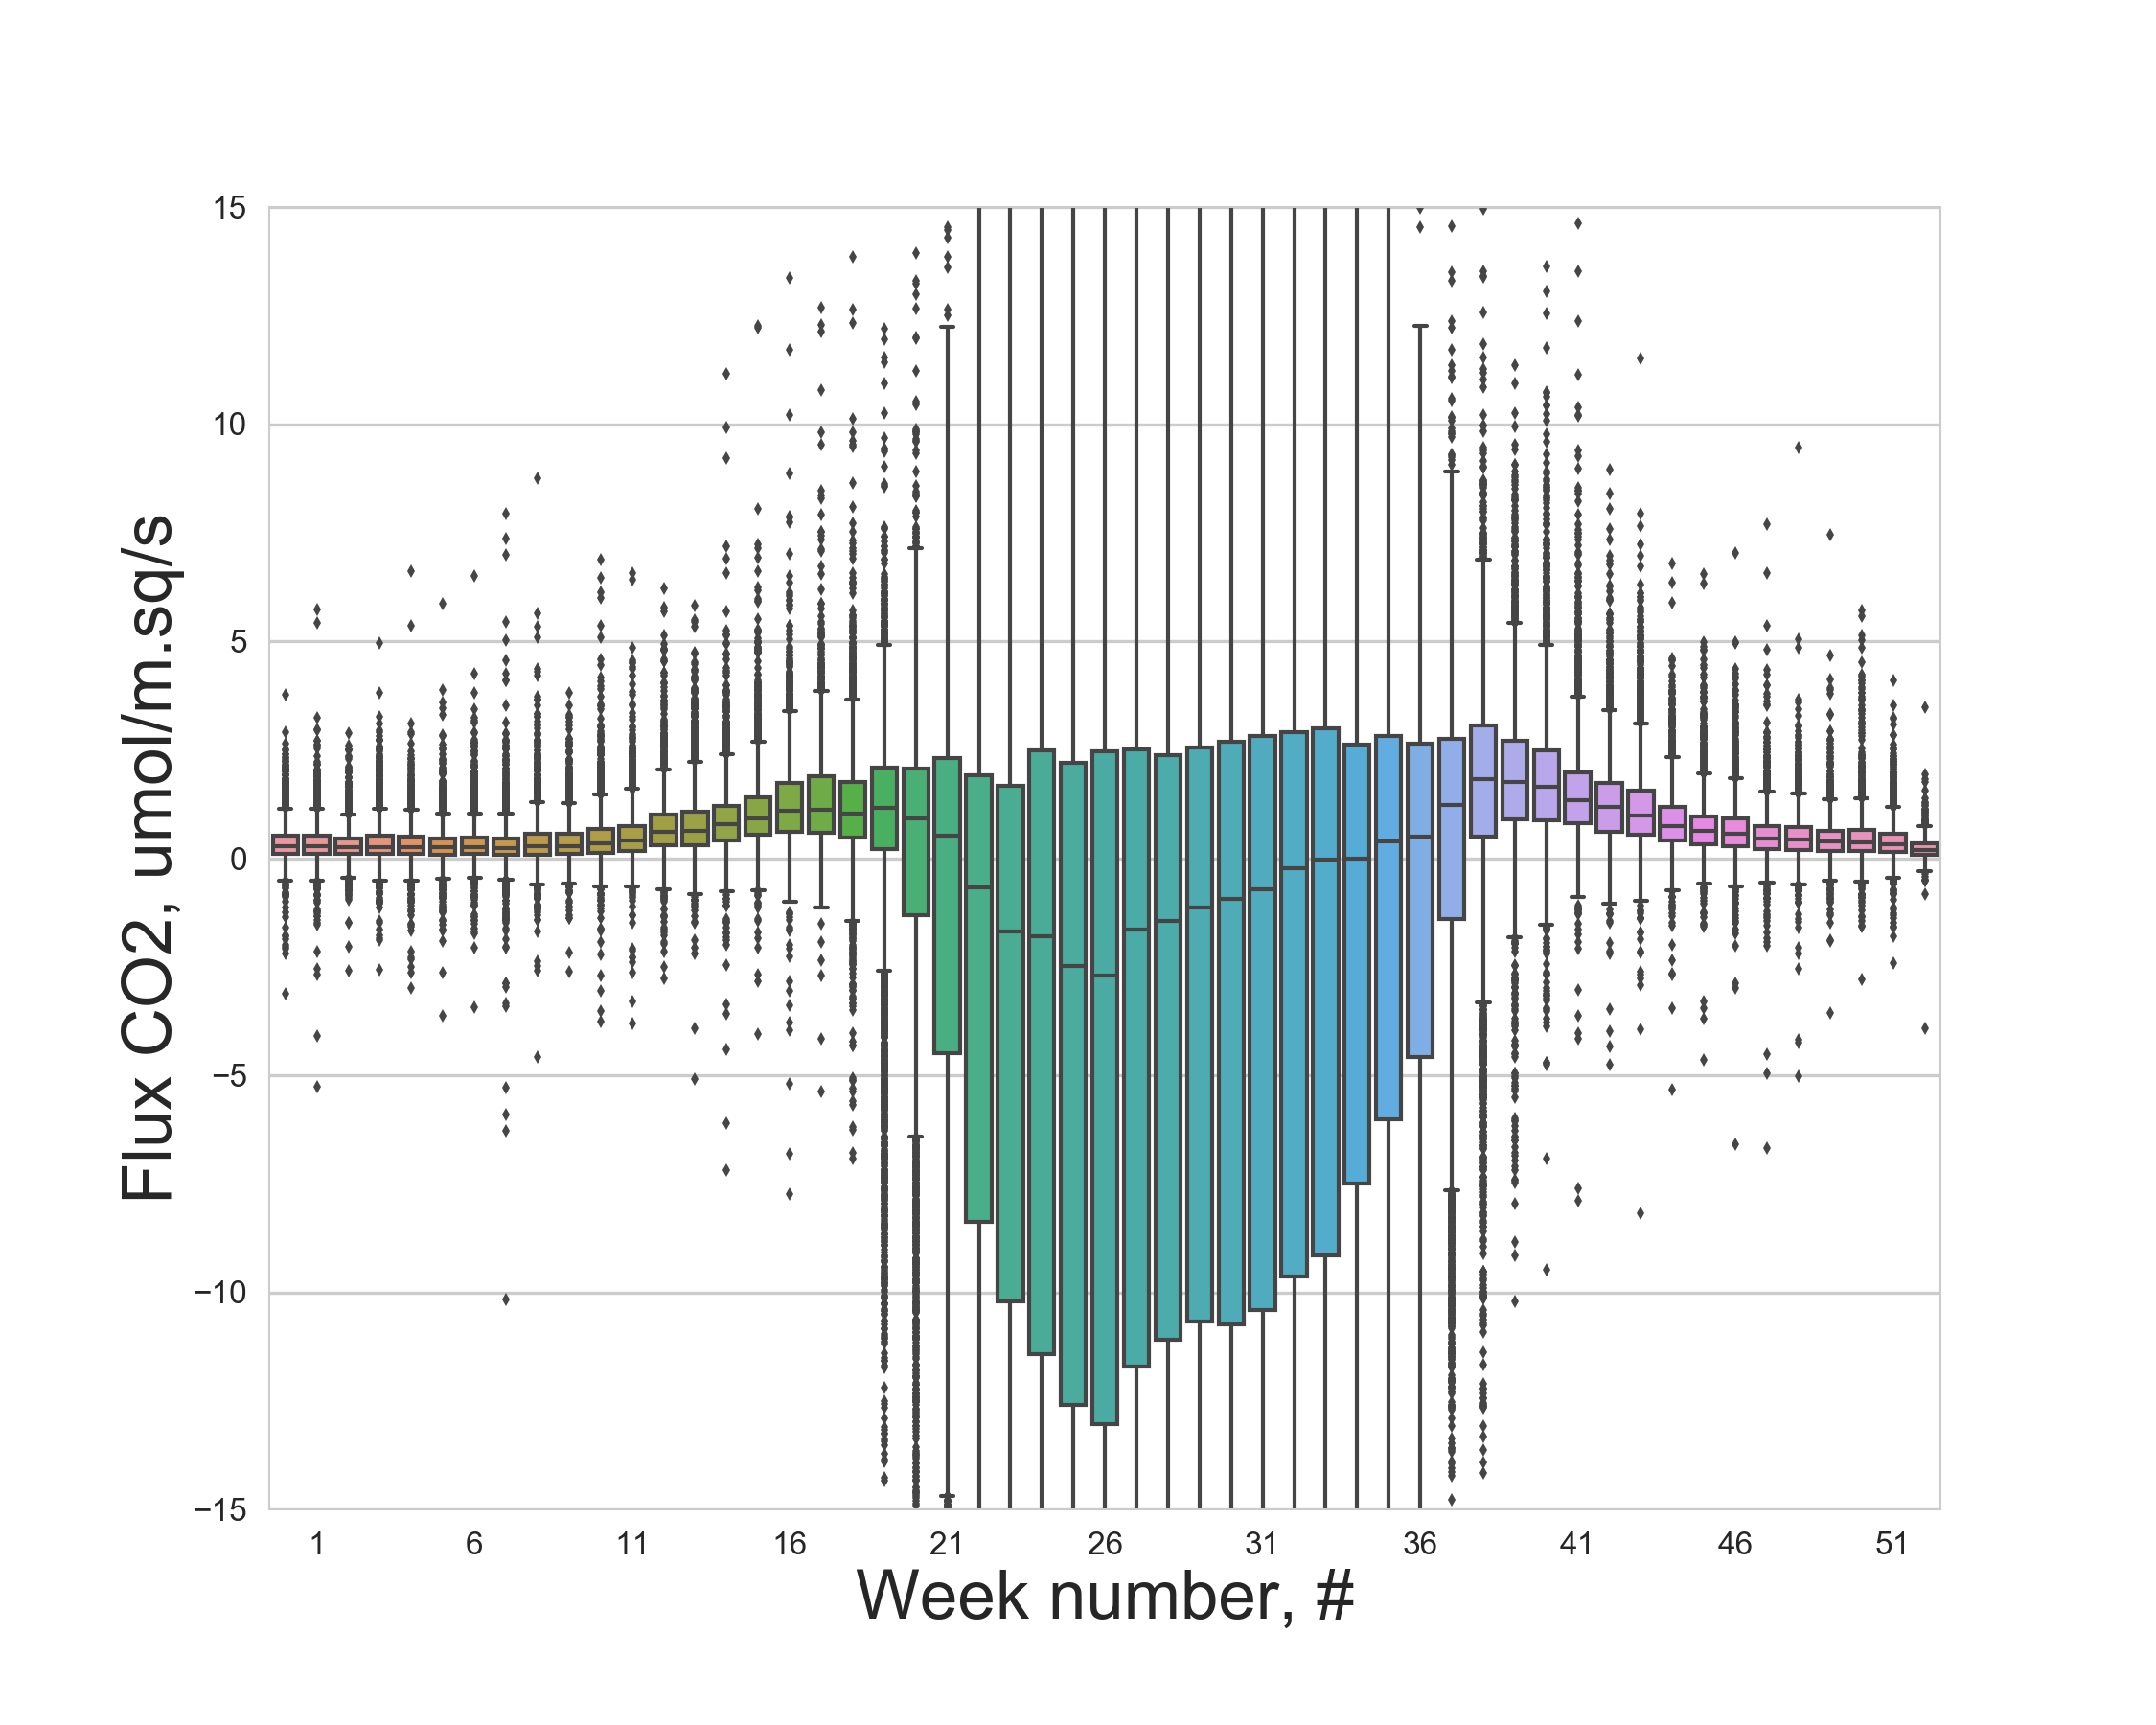
\includegraphics[width=\textwidth]{FvsW/CA-Oas.png}
% \column{.35\textwidth}
% \centering
% 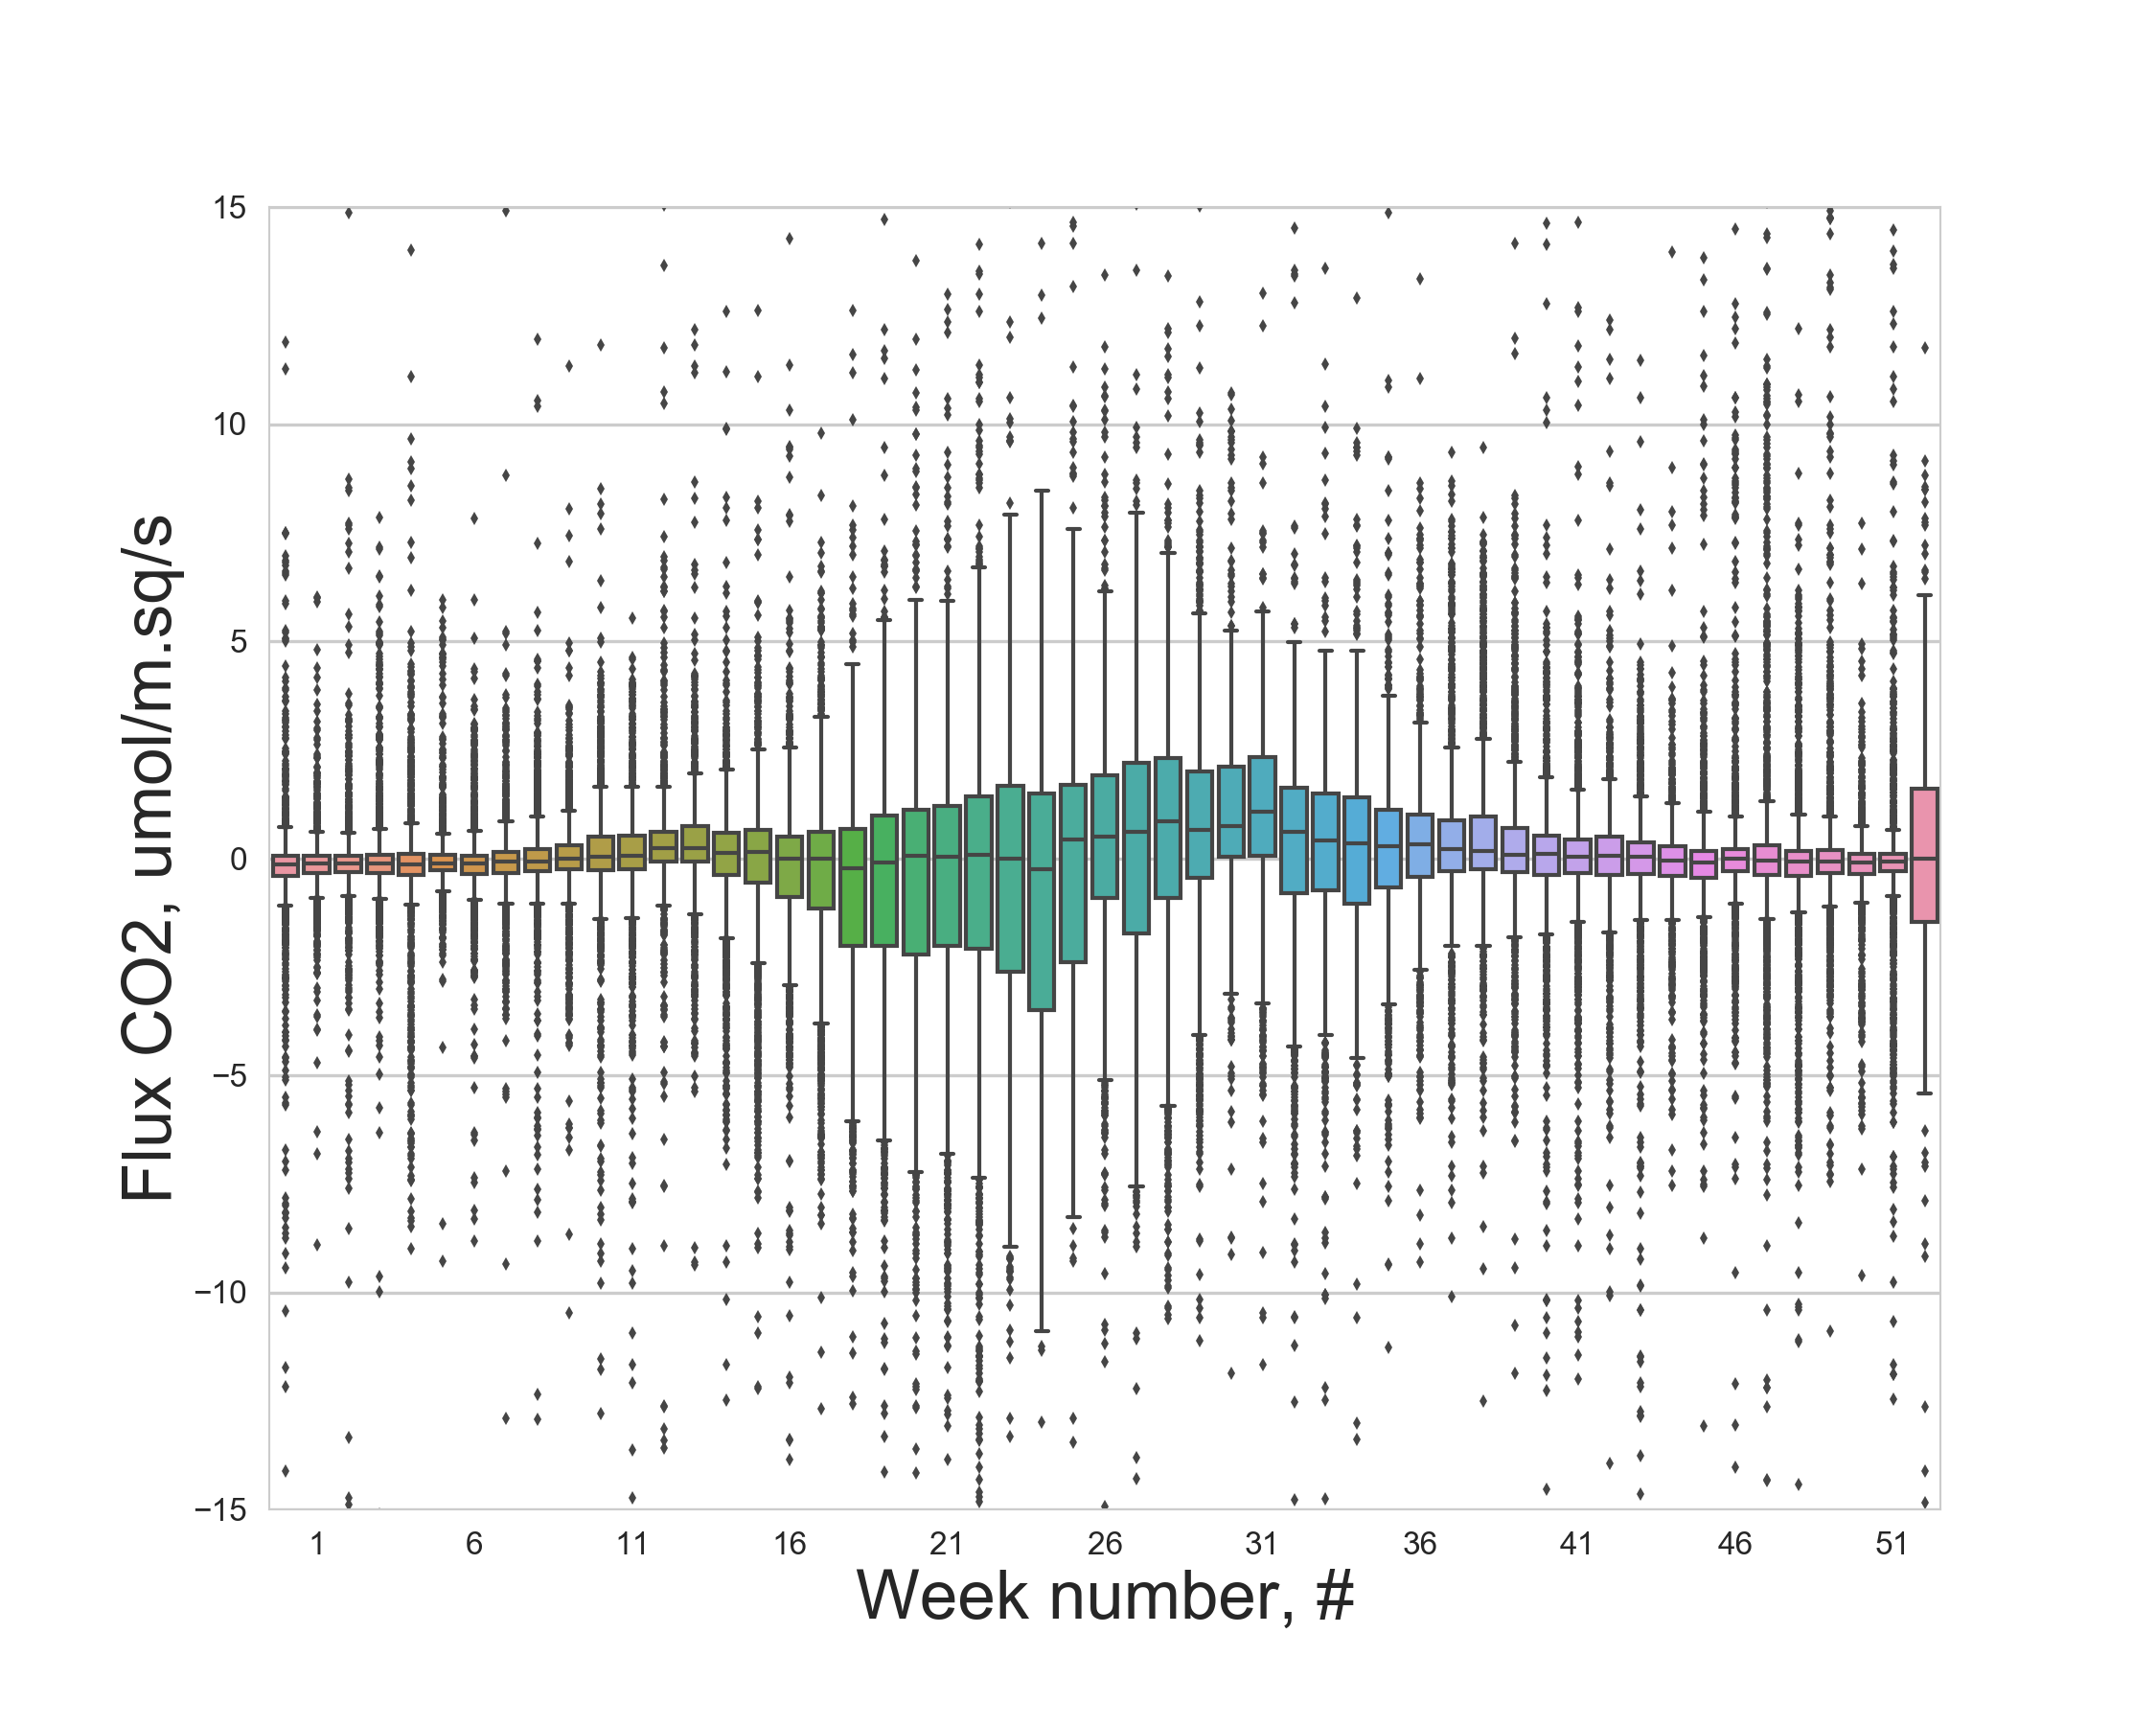
\includegraphics[width=\textwidth]{FvsW/US-FPe.png}\\
% 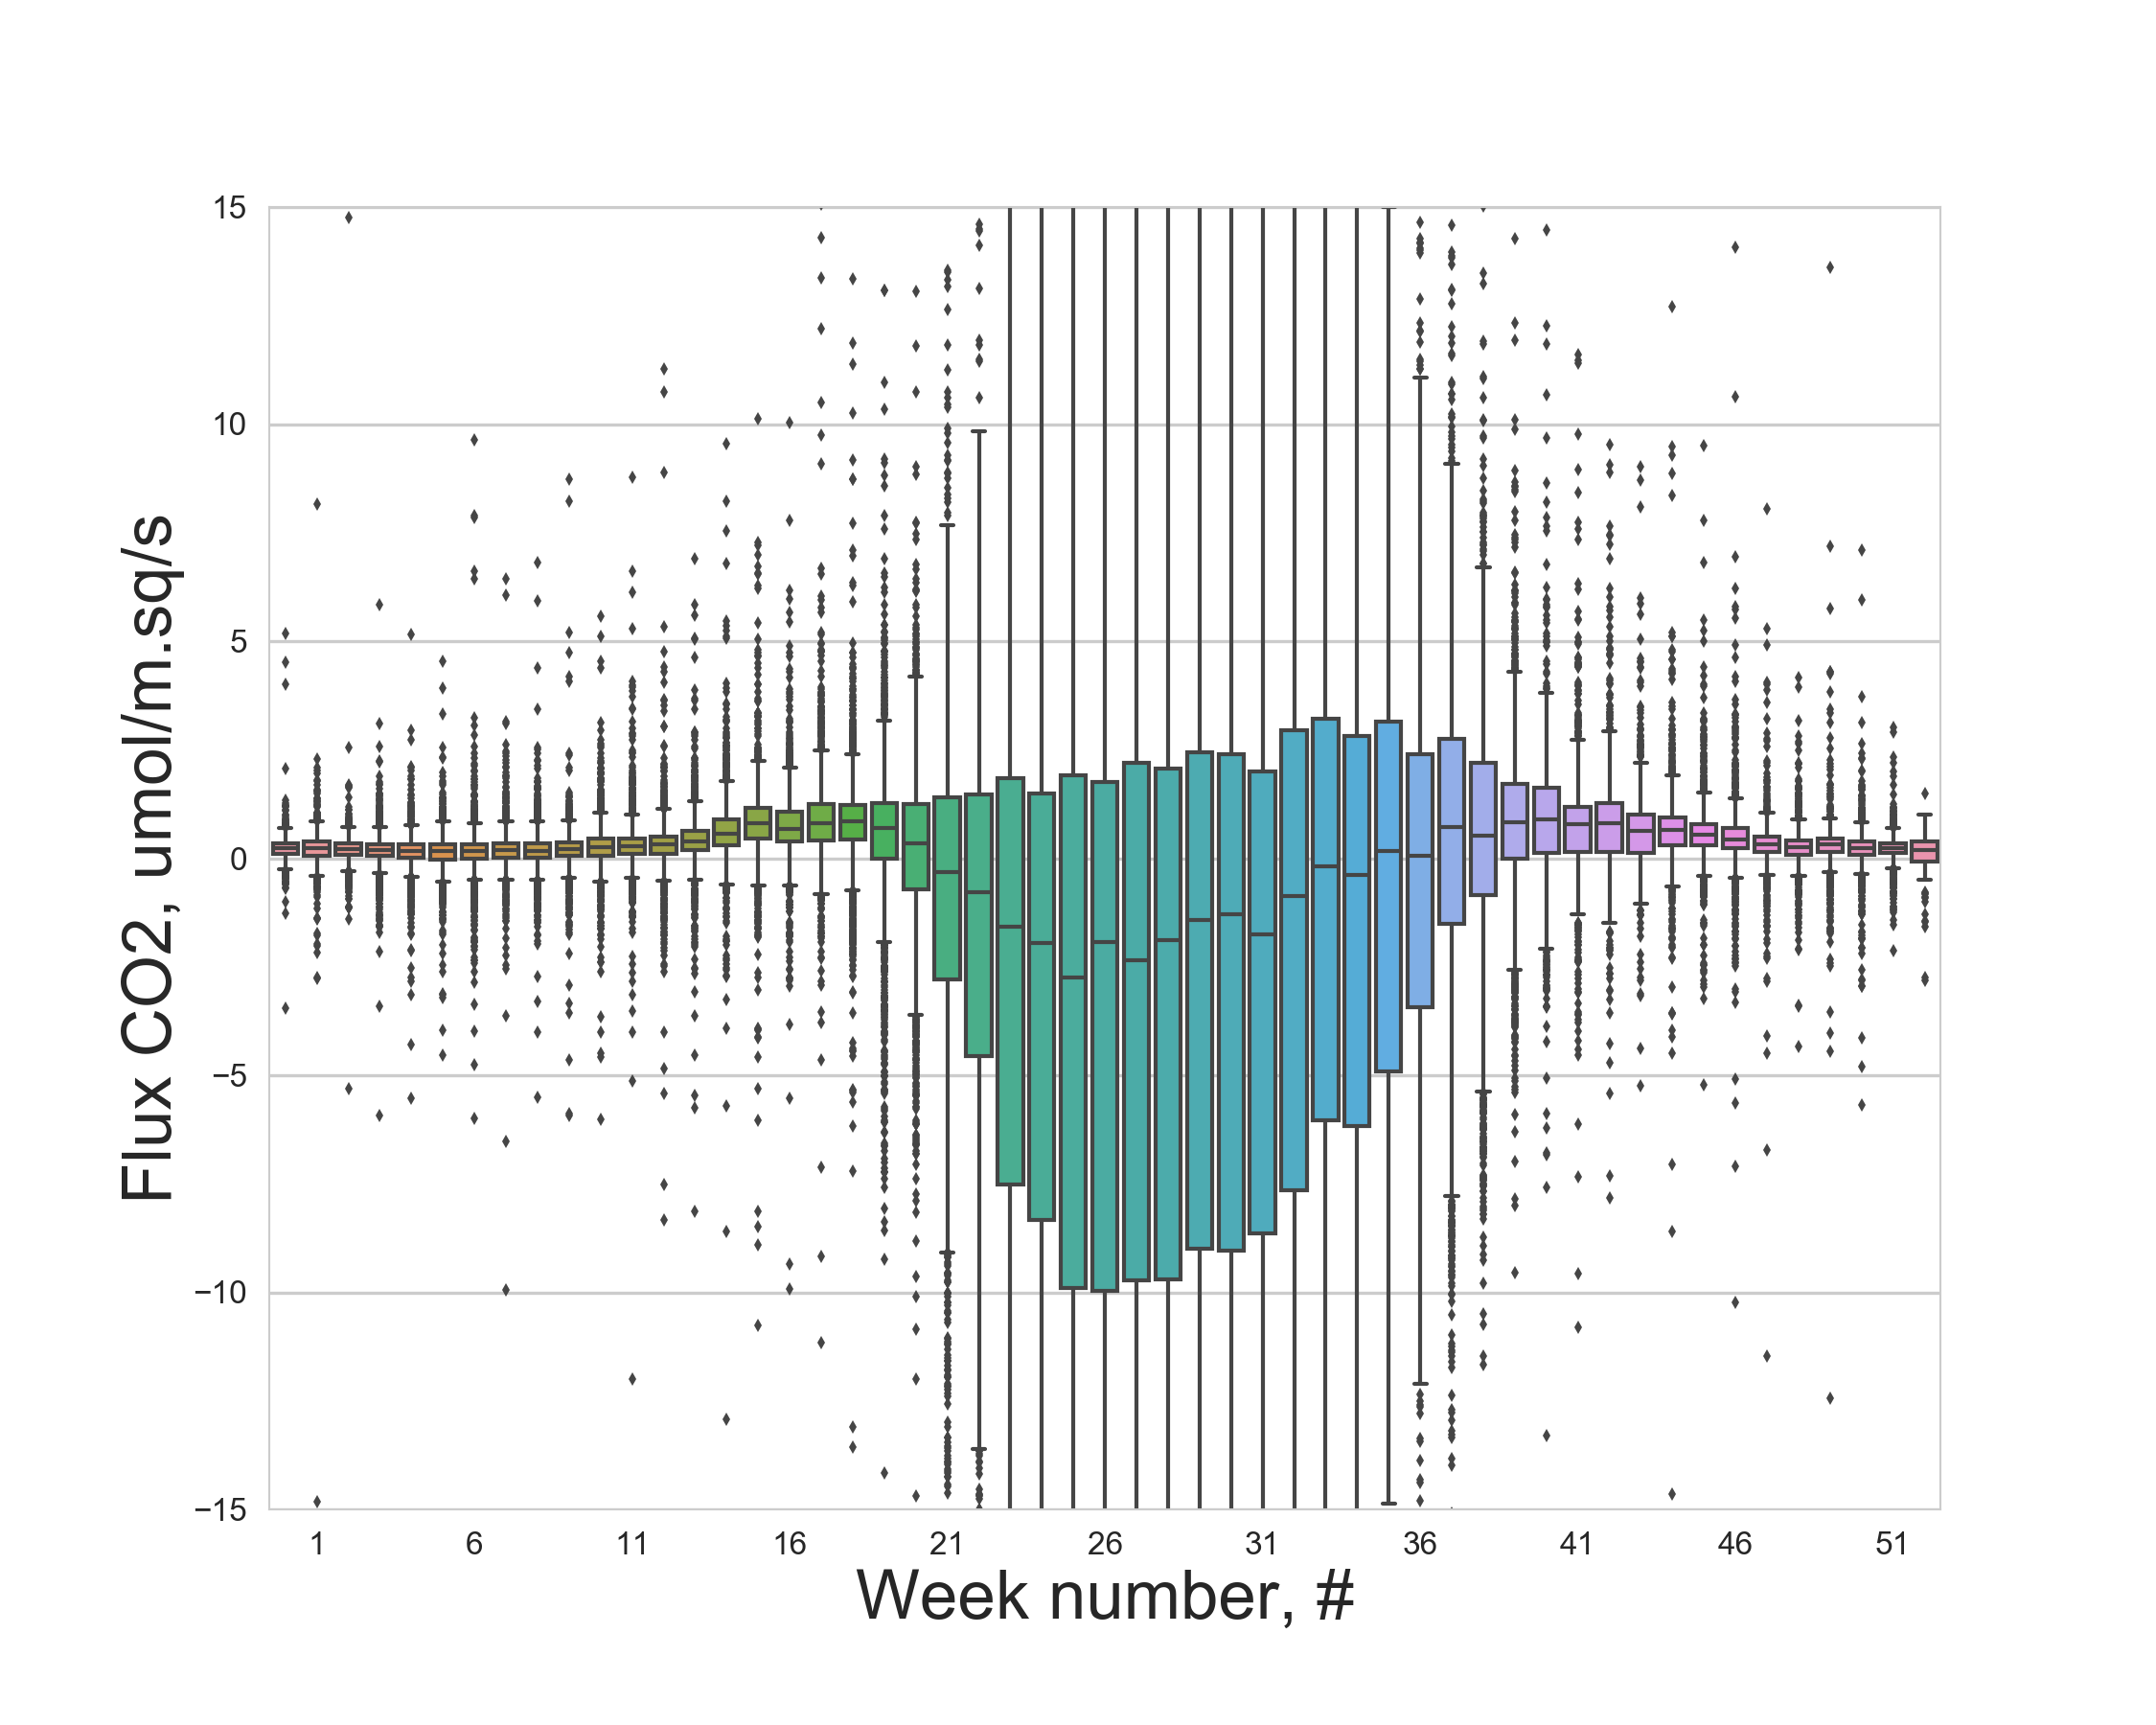
\includegraphics[width=\textwidth]{FvsW/US-Los.png}
% \end{columns}

% \end{frame}

\begin{frame}
\frametitle{Weekly average plots}
\centering
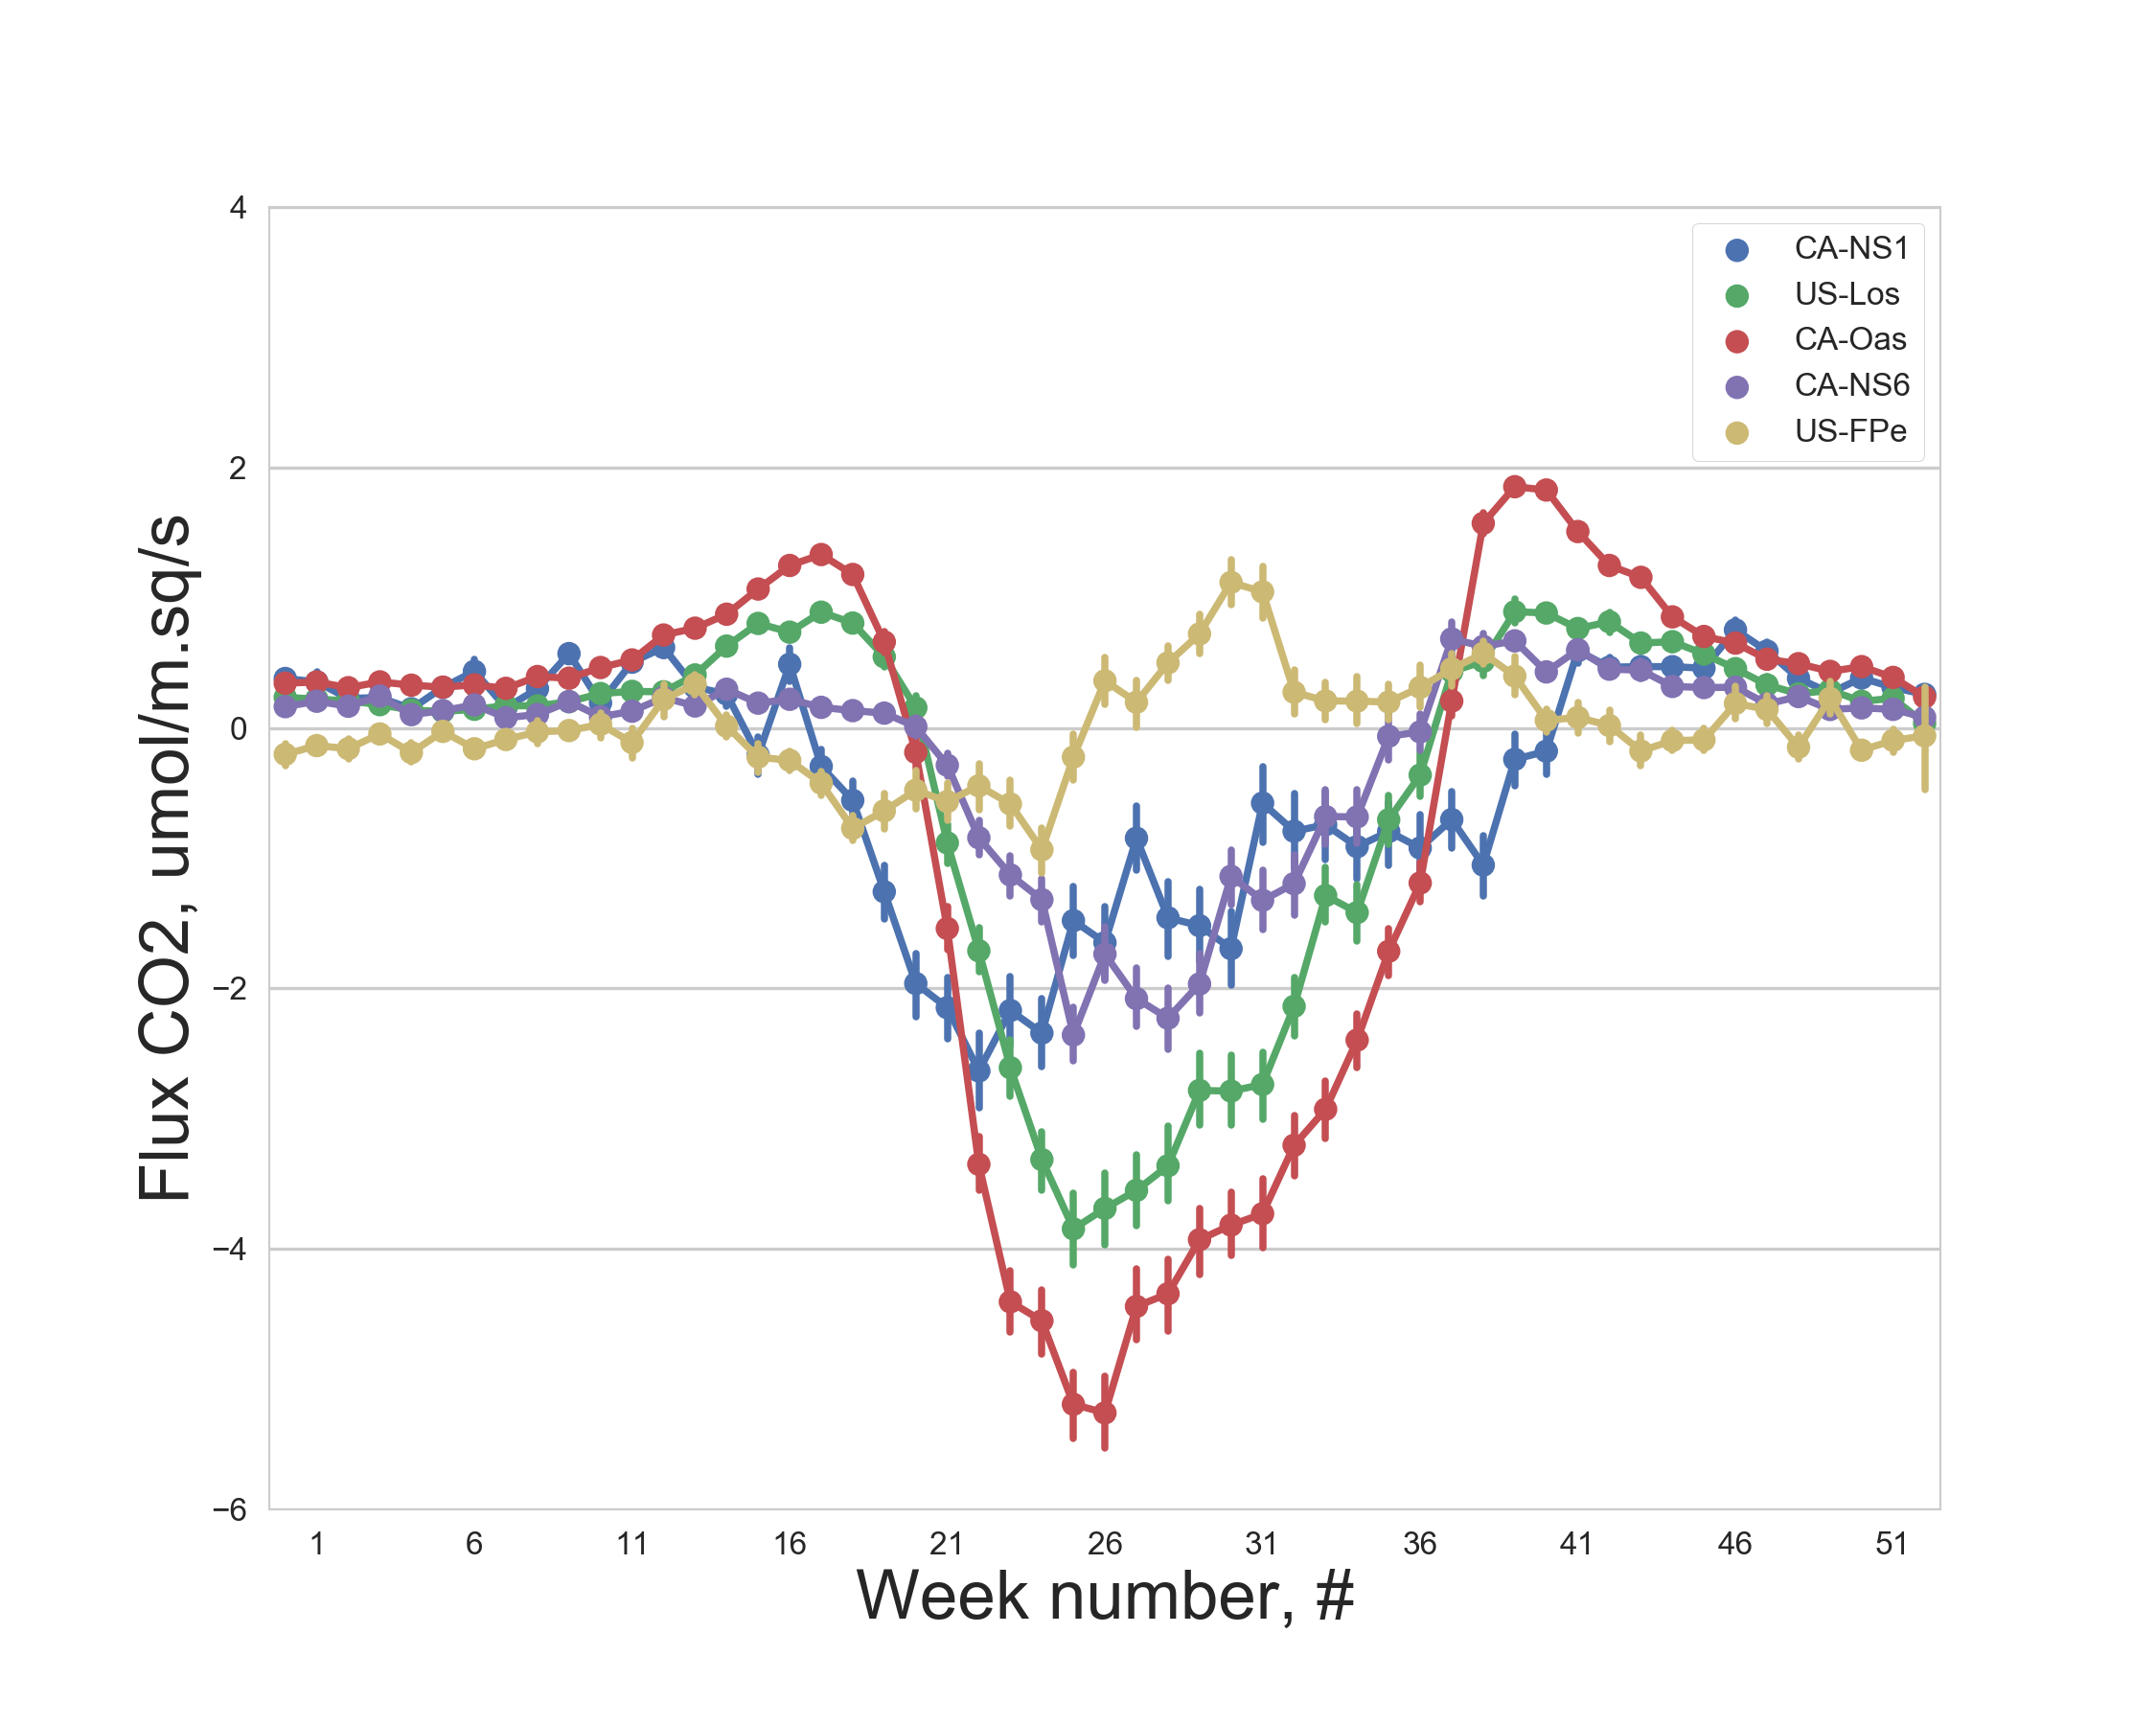
\includegraphics[width=0.9\textwidth]{FvsW_mean/all.png}\\
\end{frame}

\begin{frame}
\frametitle{Weekly average: Day/Night}

\begin{columns}[t]
\column{.35\textwidth}
\centering
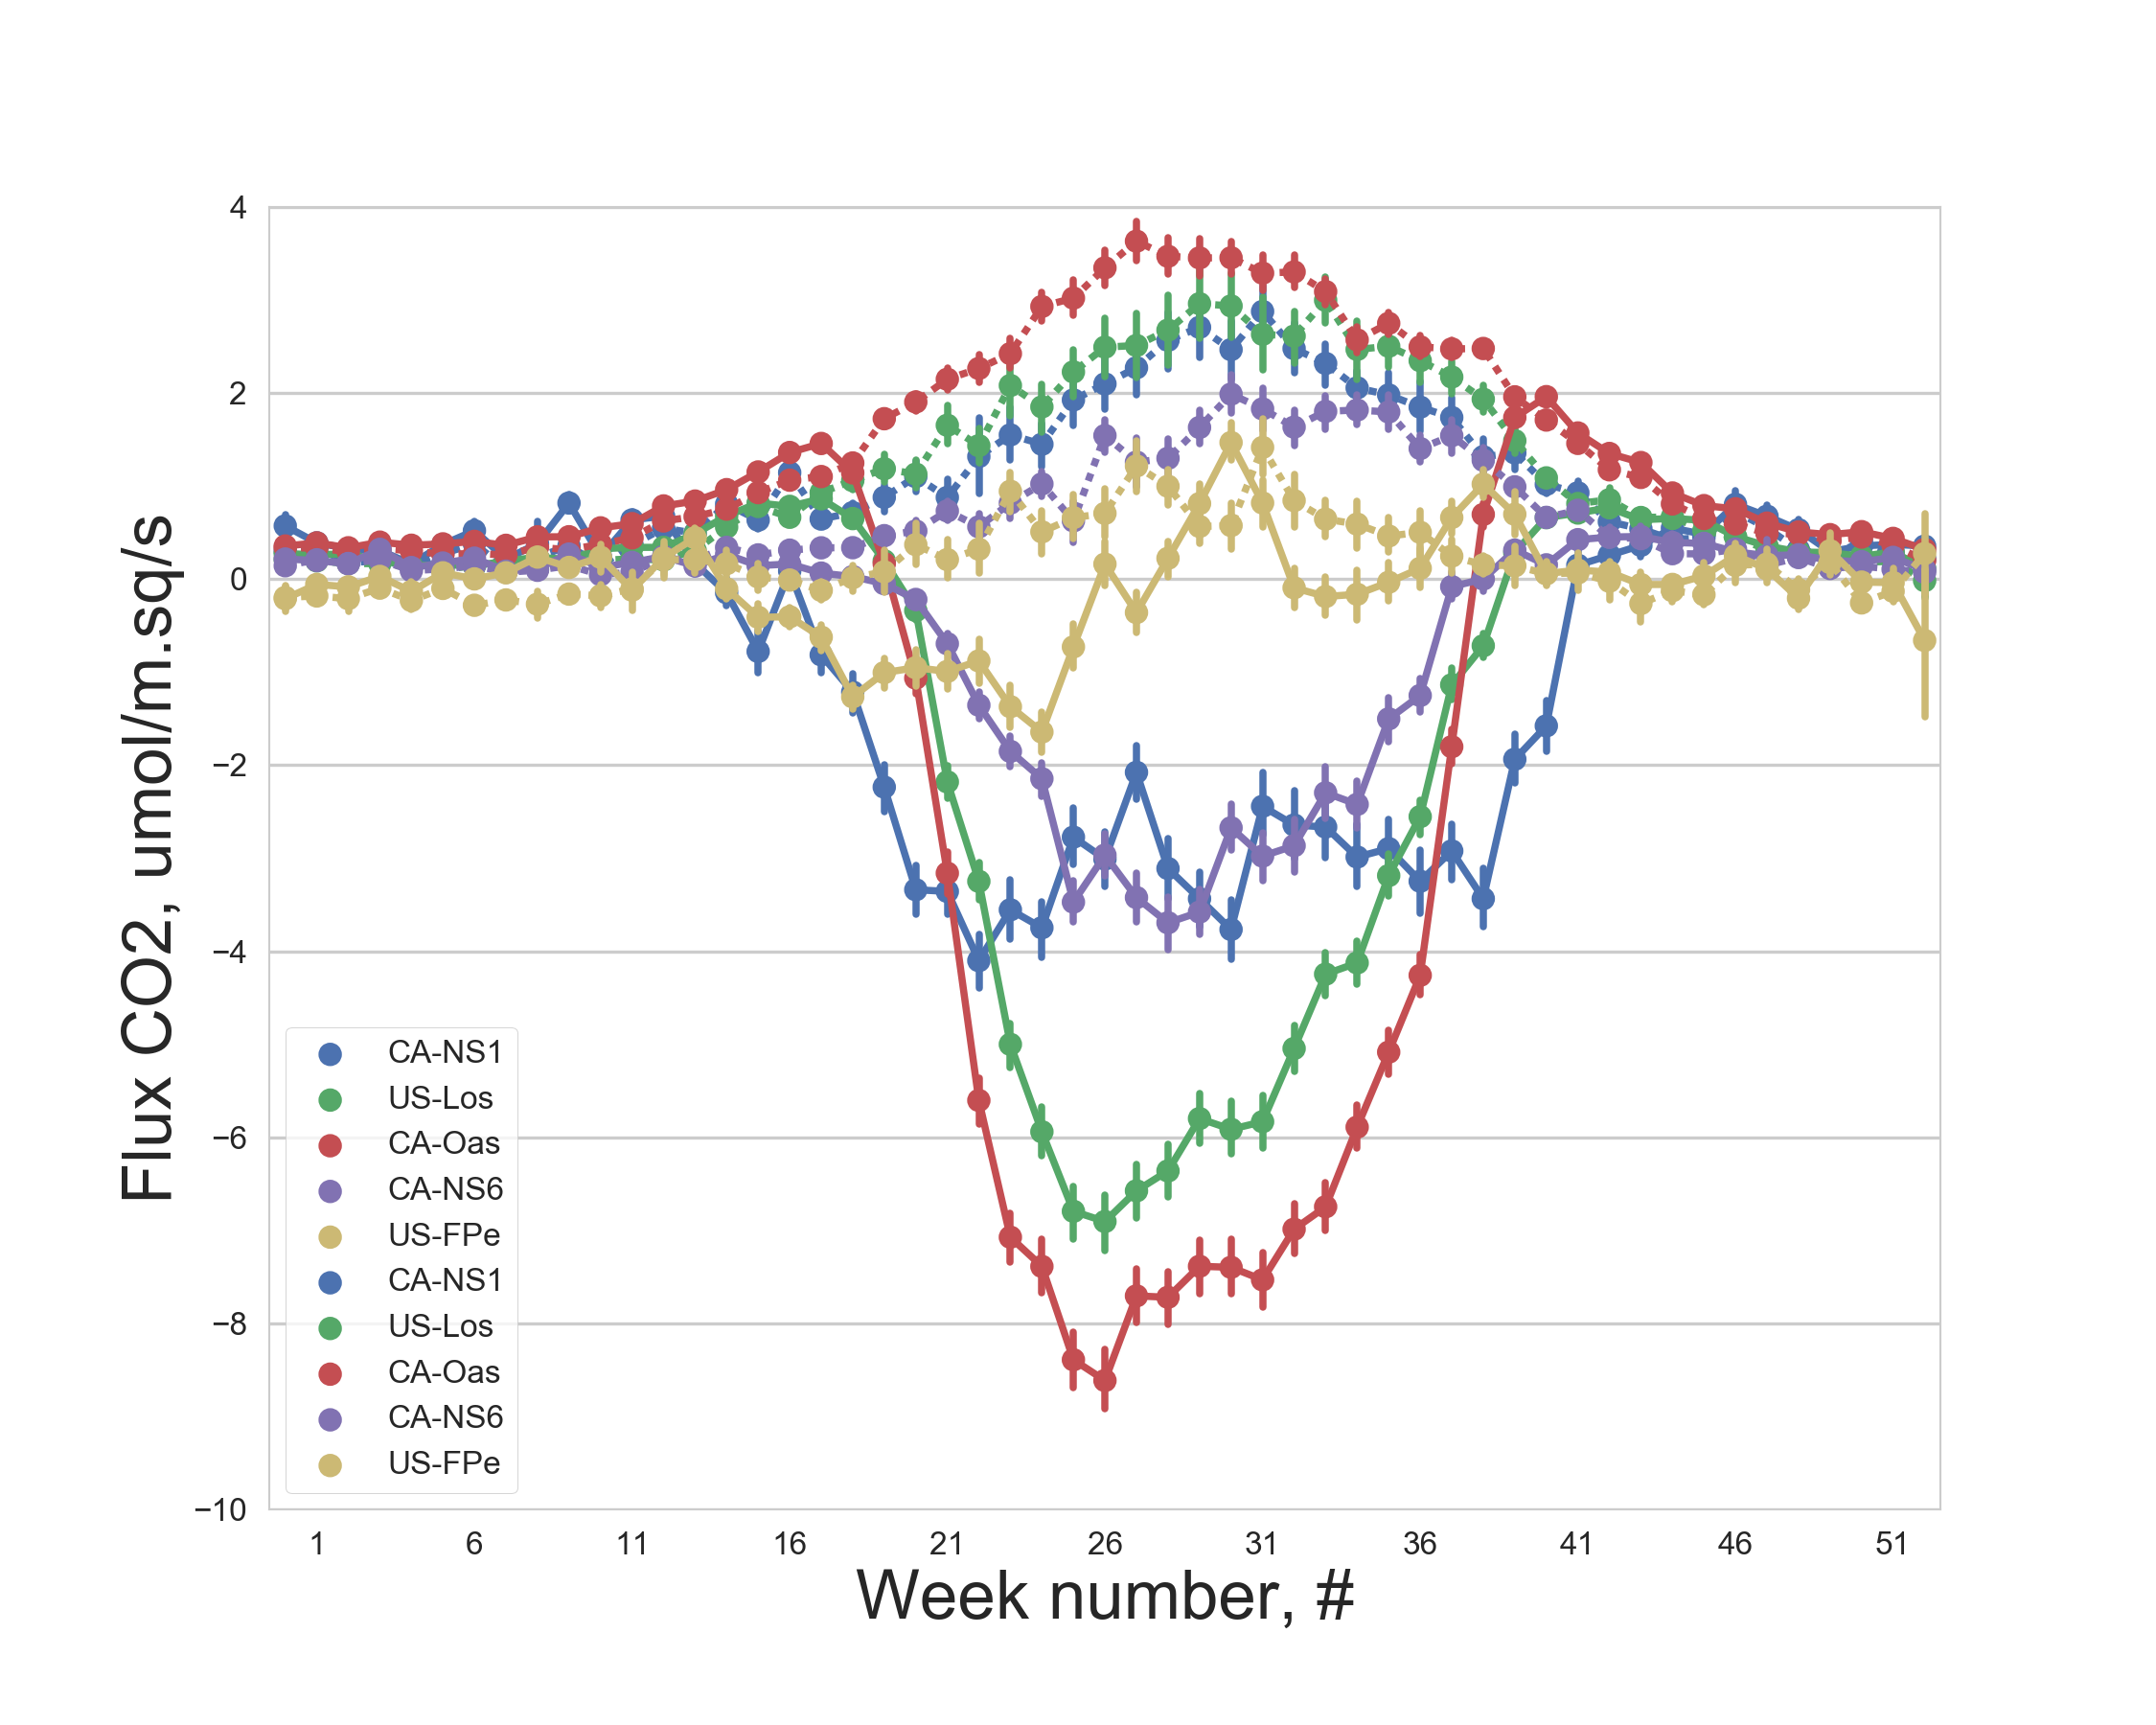
\includegraphics[width=\textwidth]{FvsW_day/all.png}\\
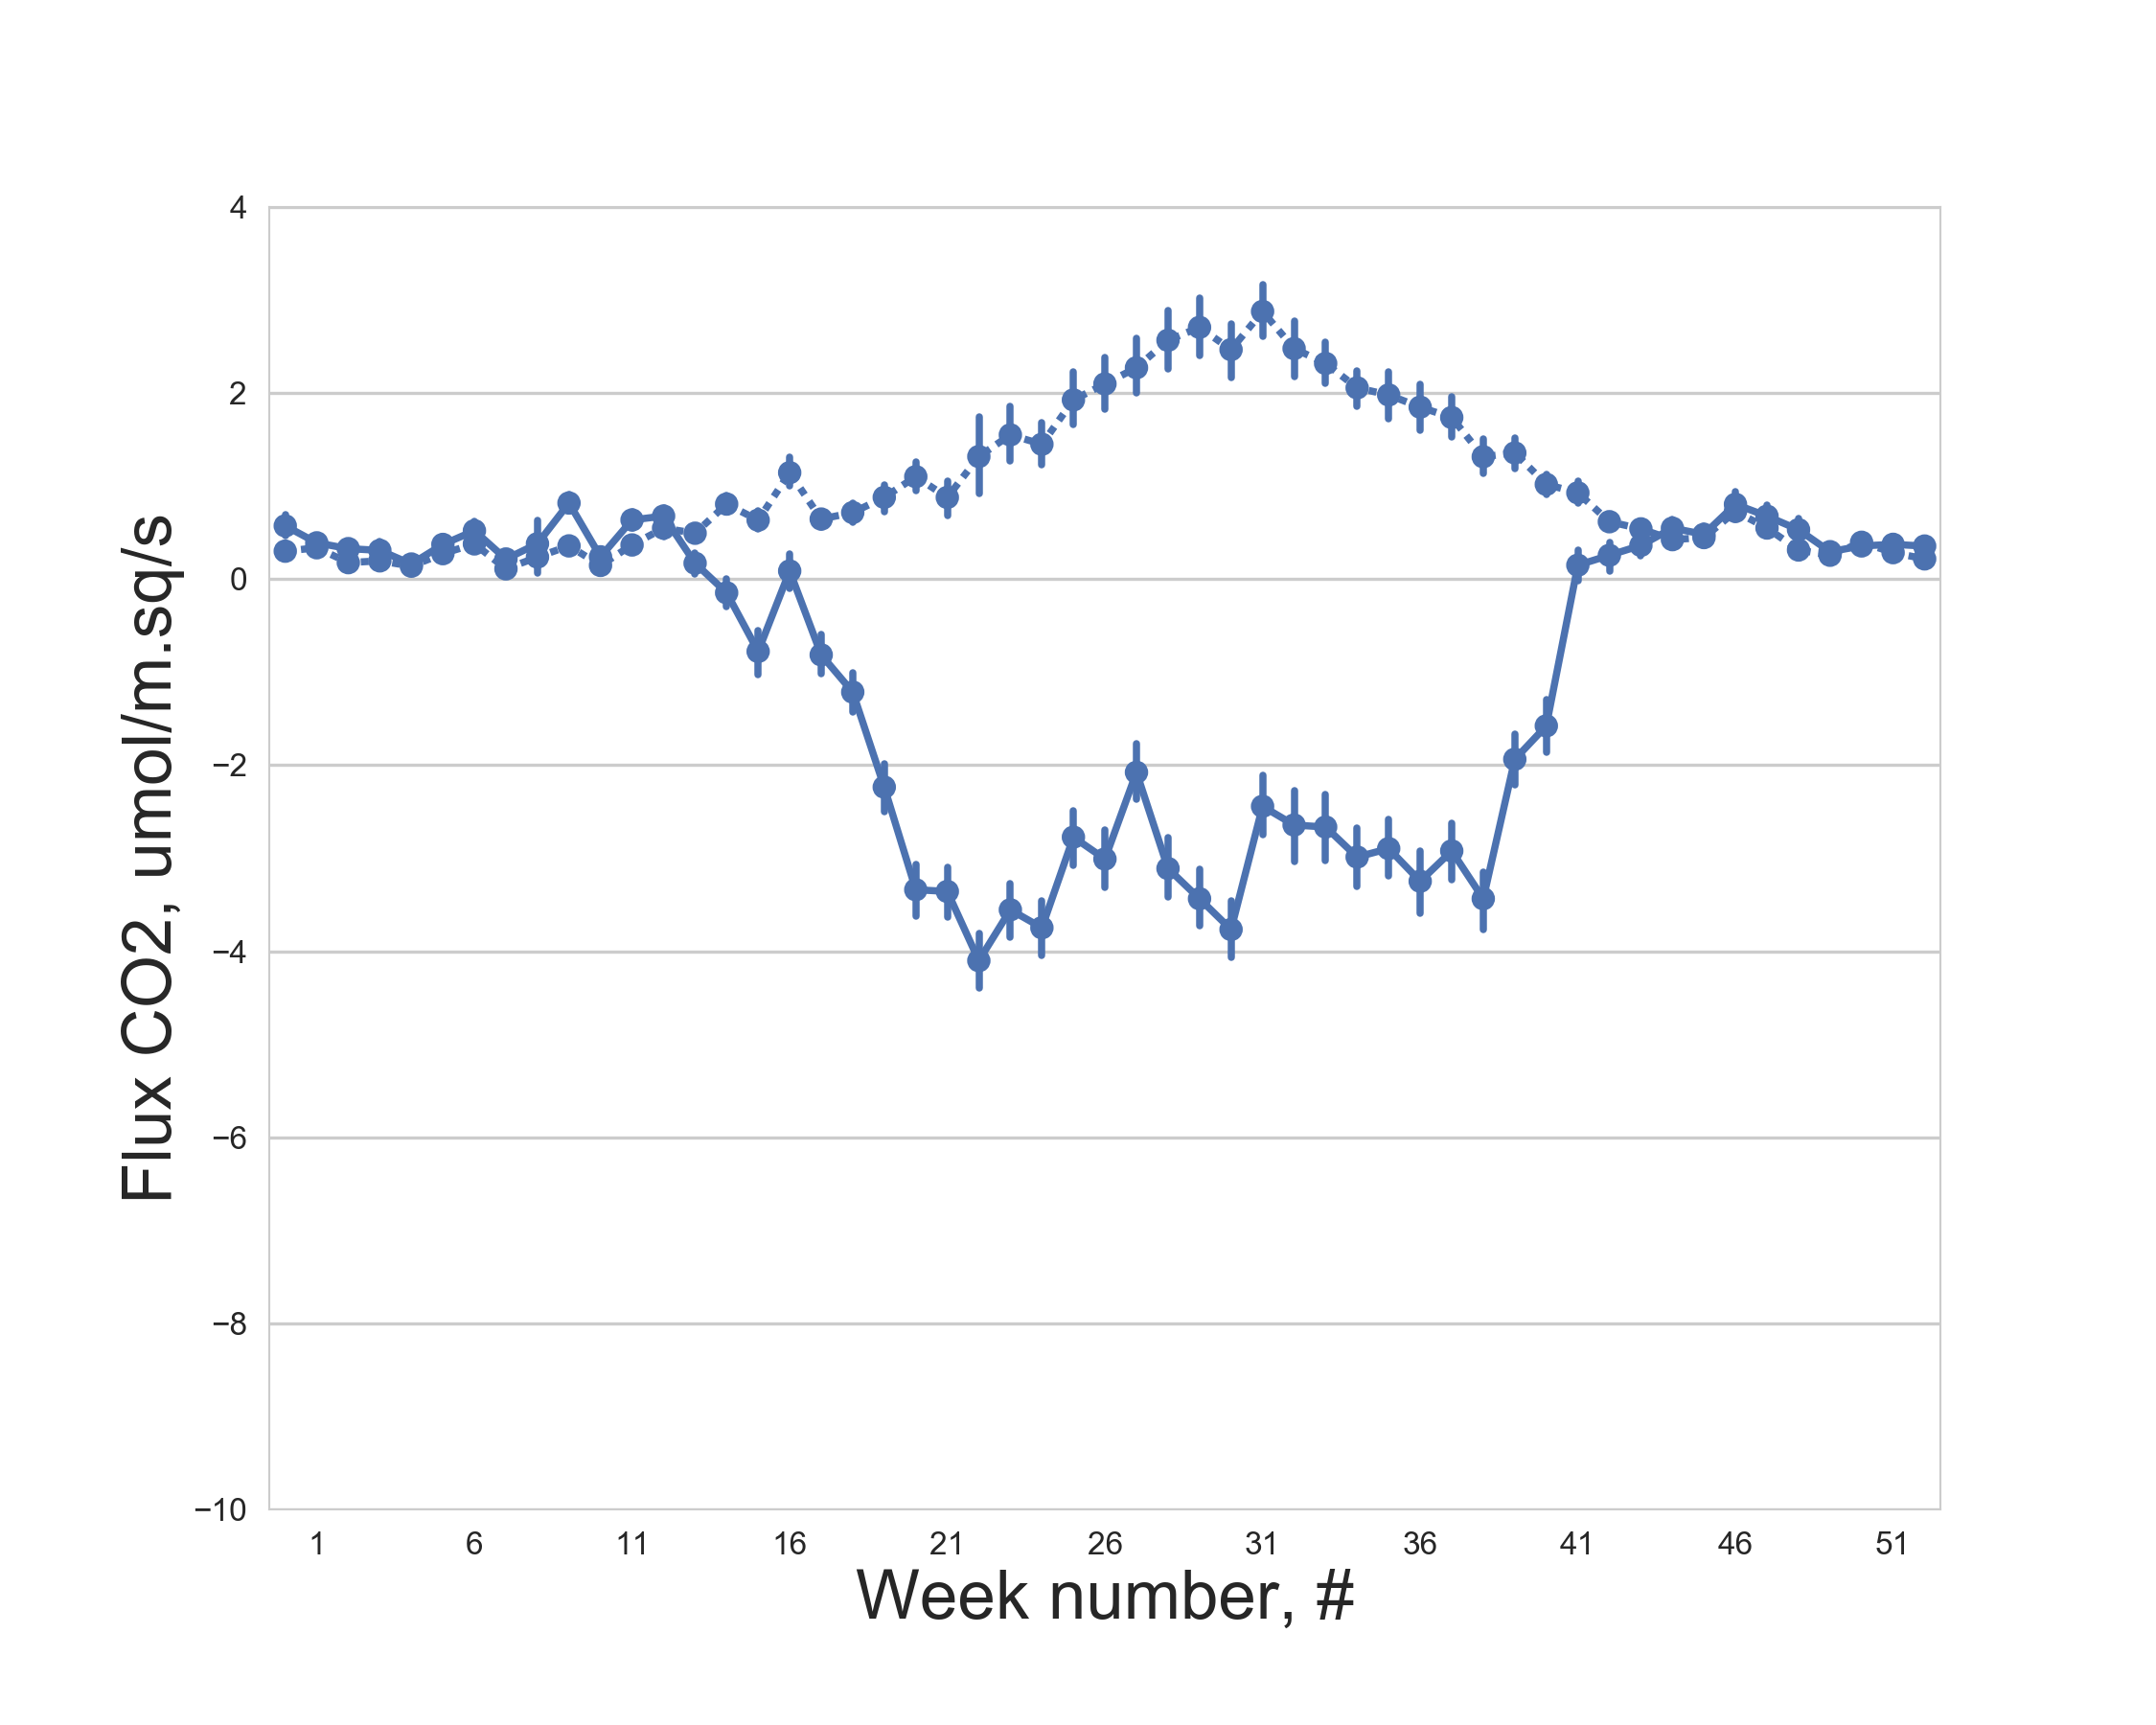
\includegraphics[width=\textwidth]{FvsW_day/CA-NS1.png}
\column{.35\textwidth}
\centering
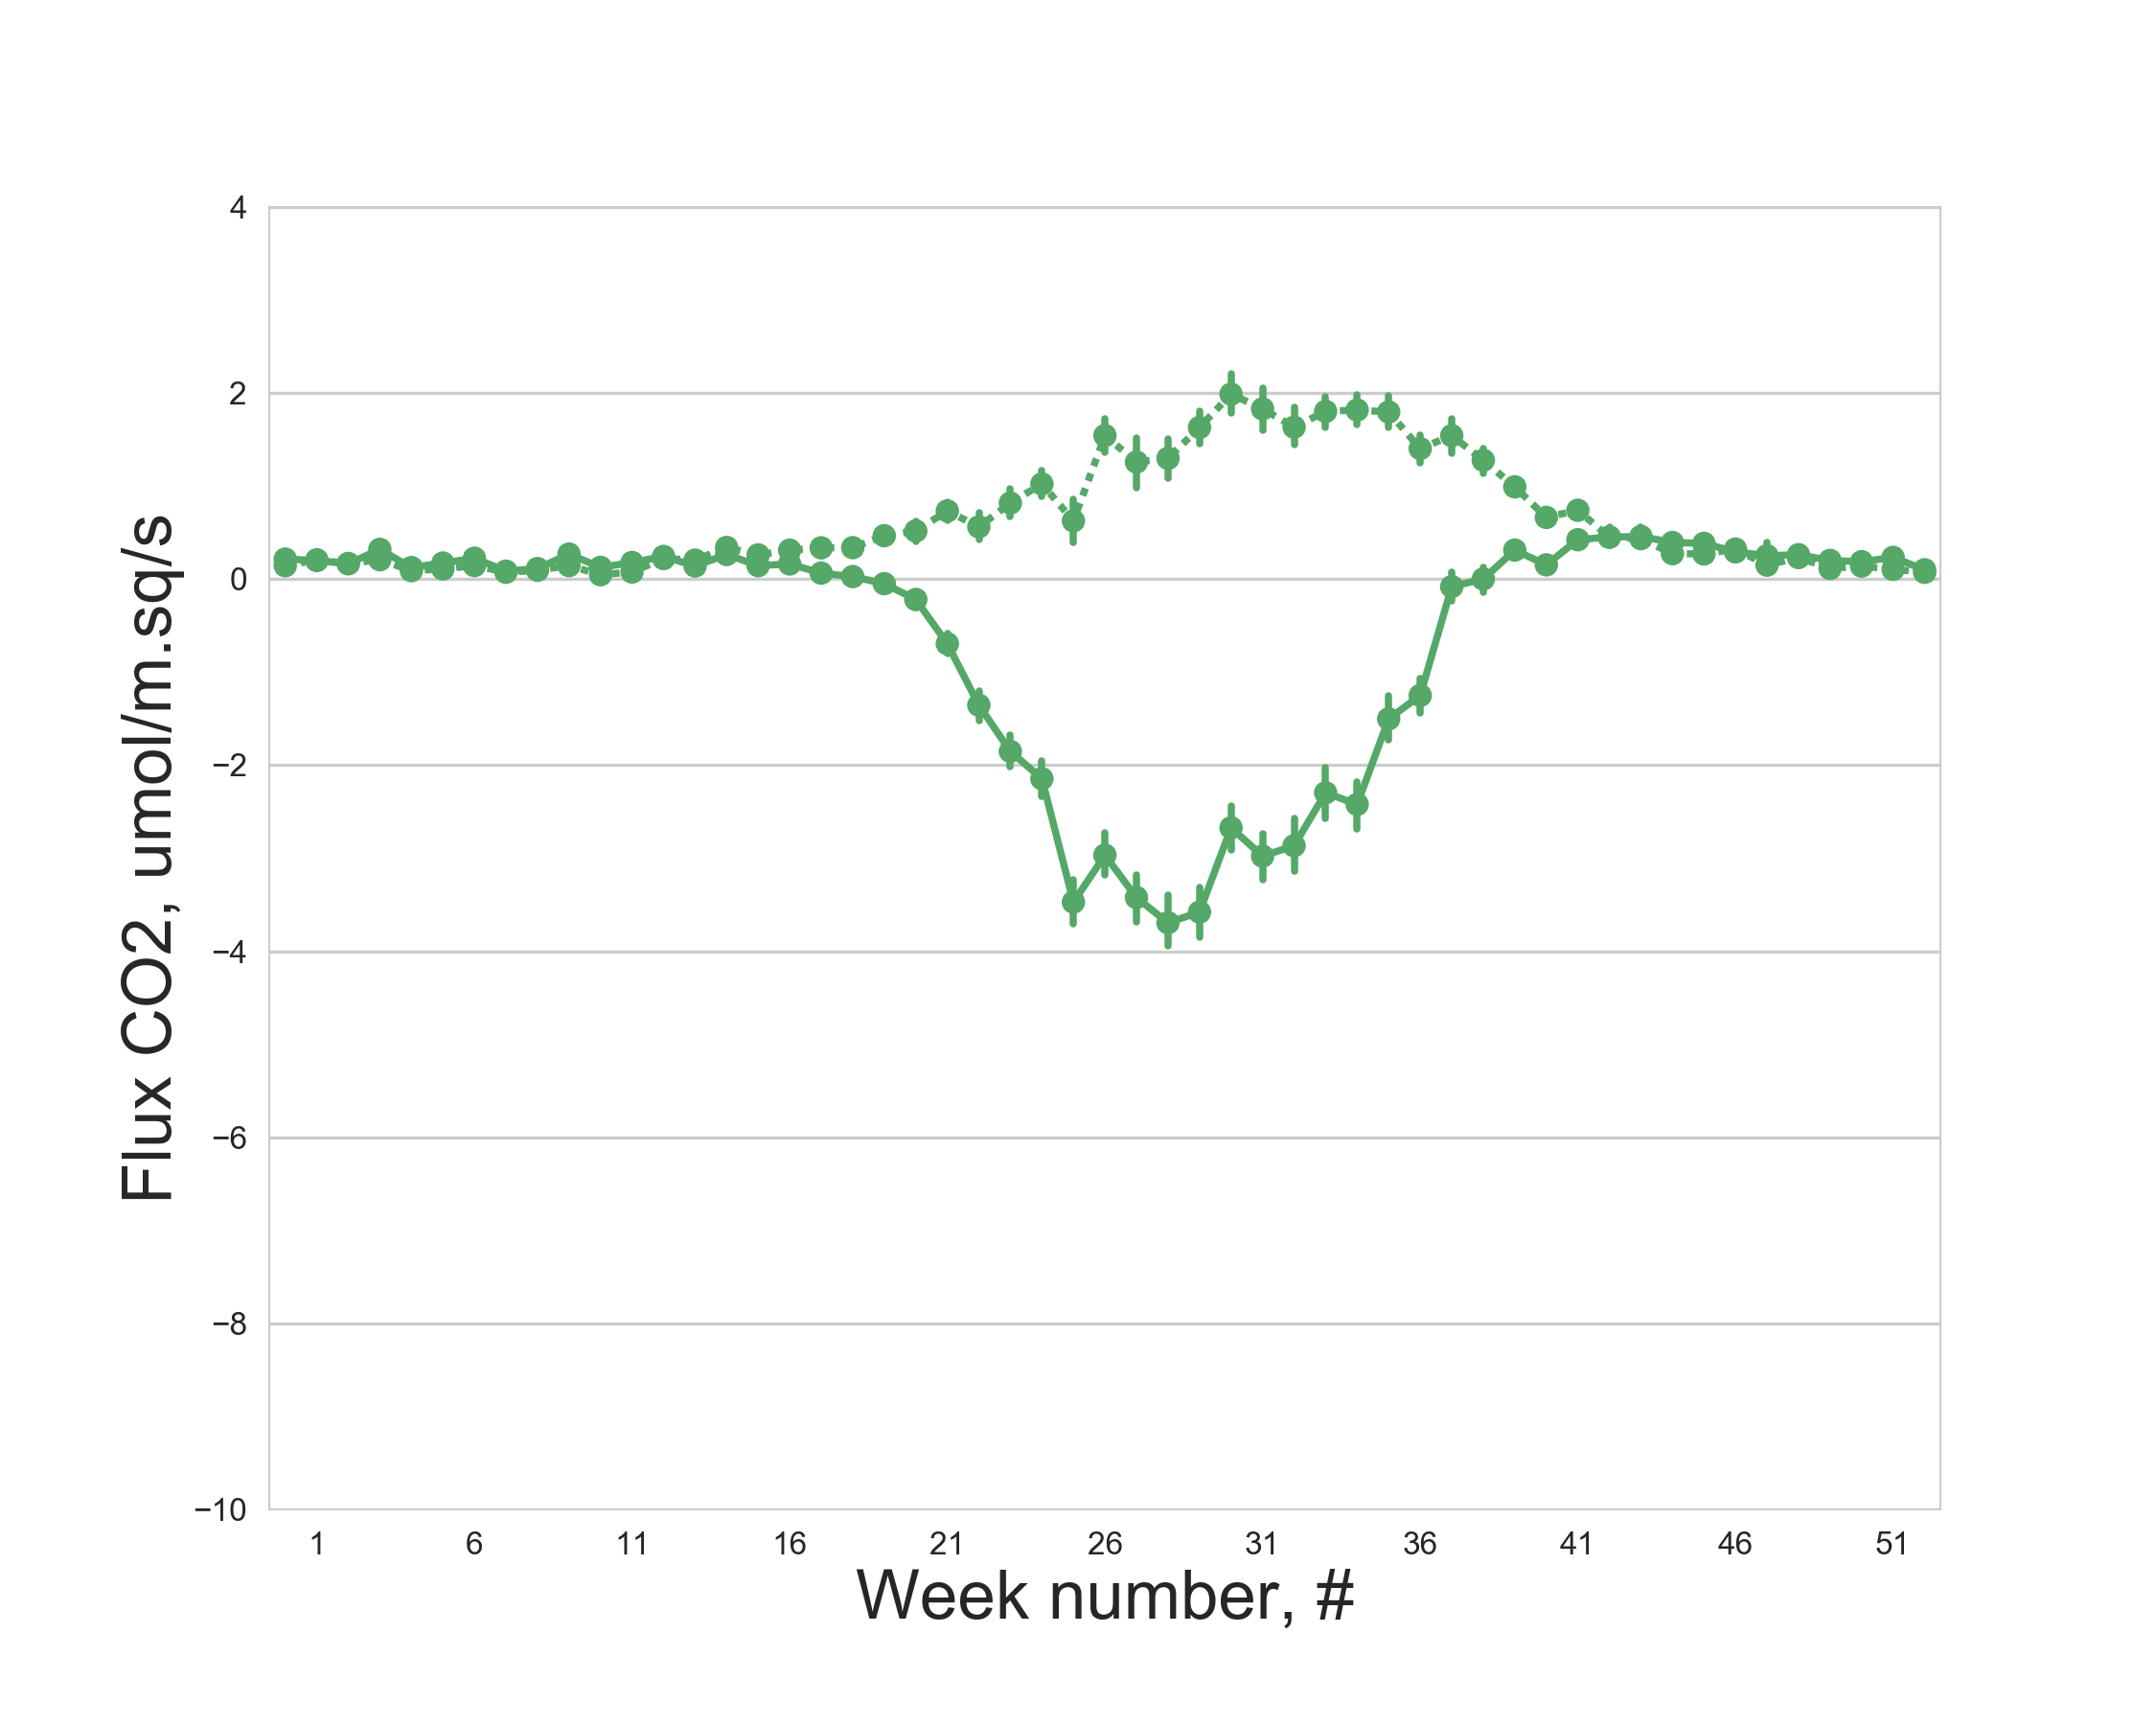
\includegraphics[width=\textwidth]{FvsW_day/CA-NS6.png}\\
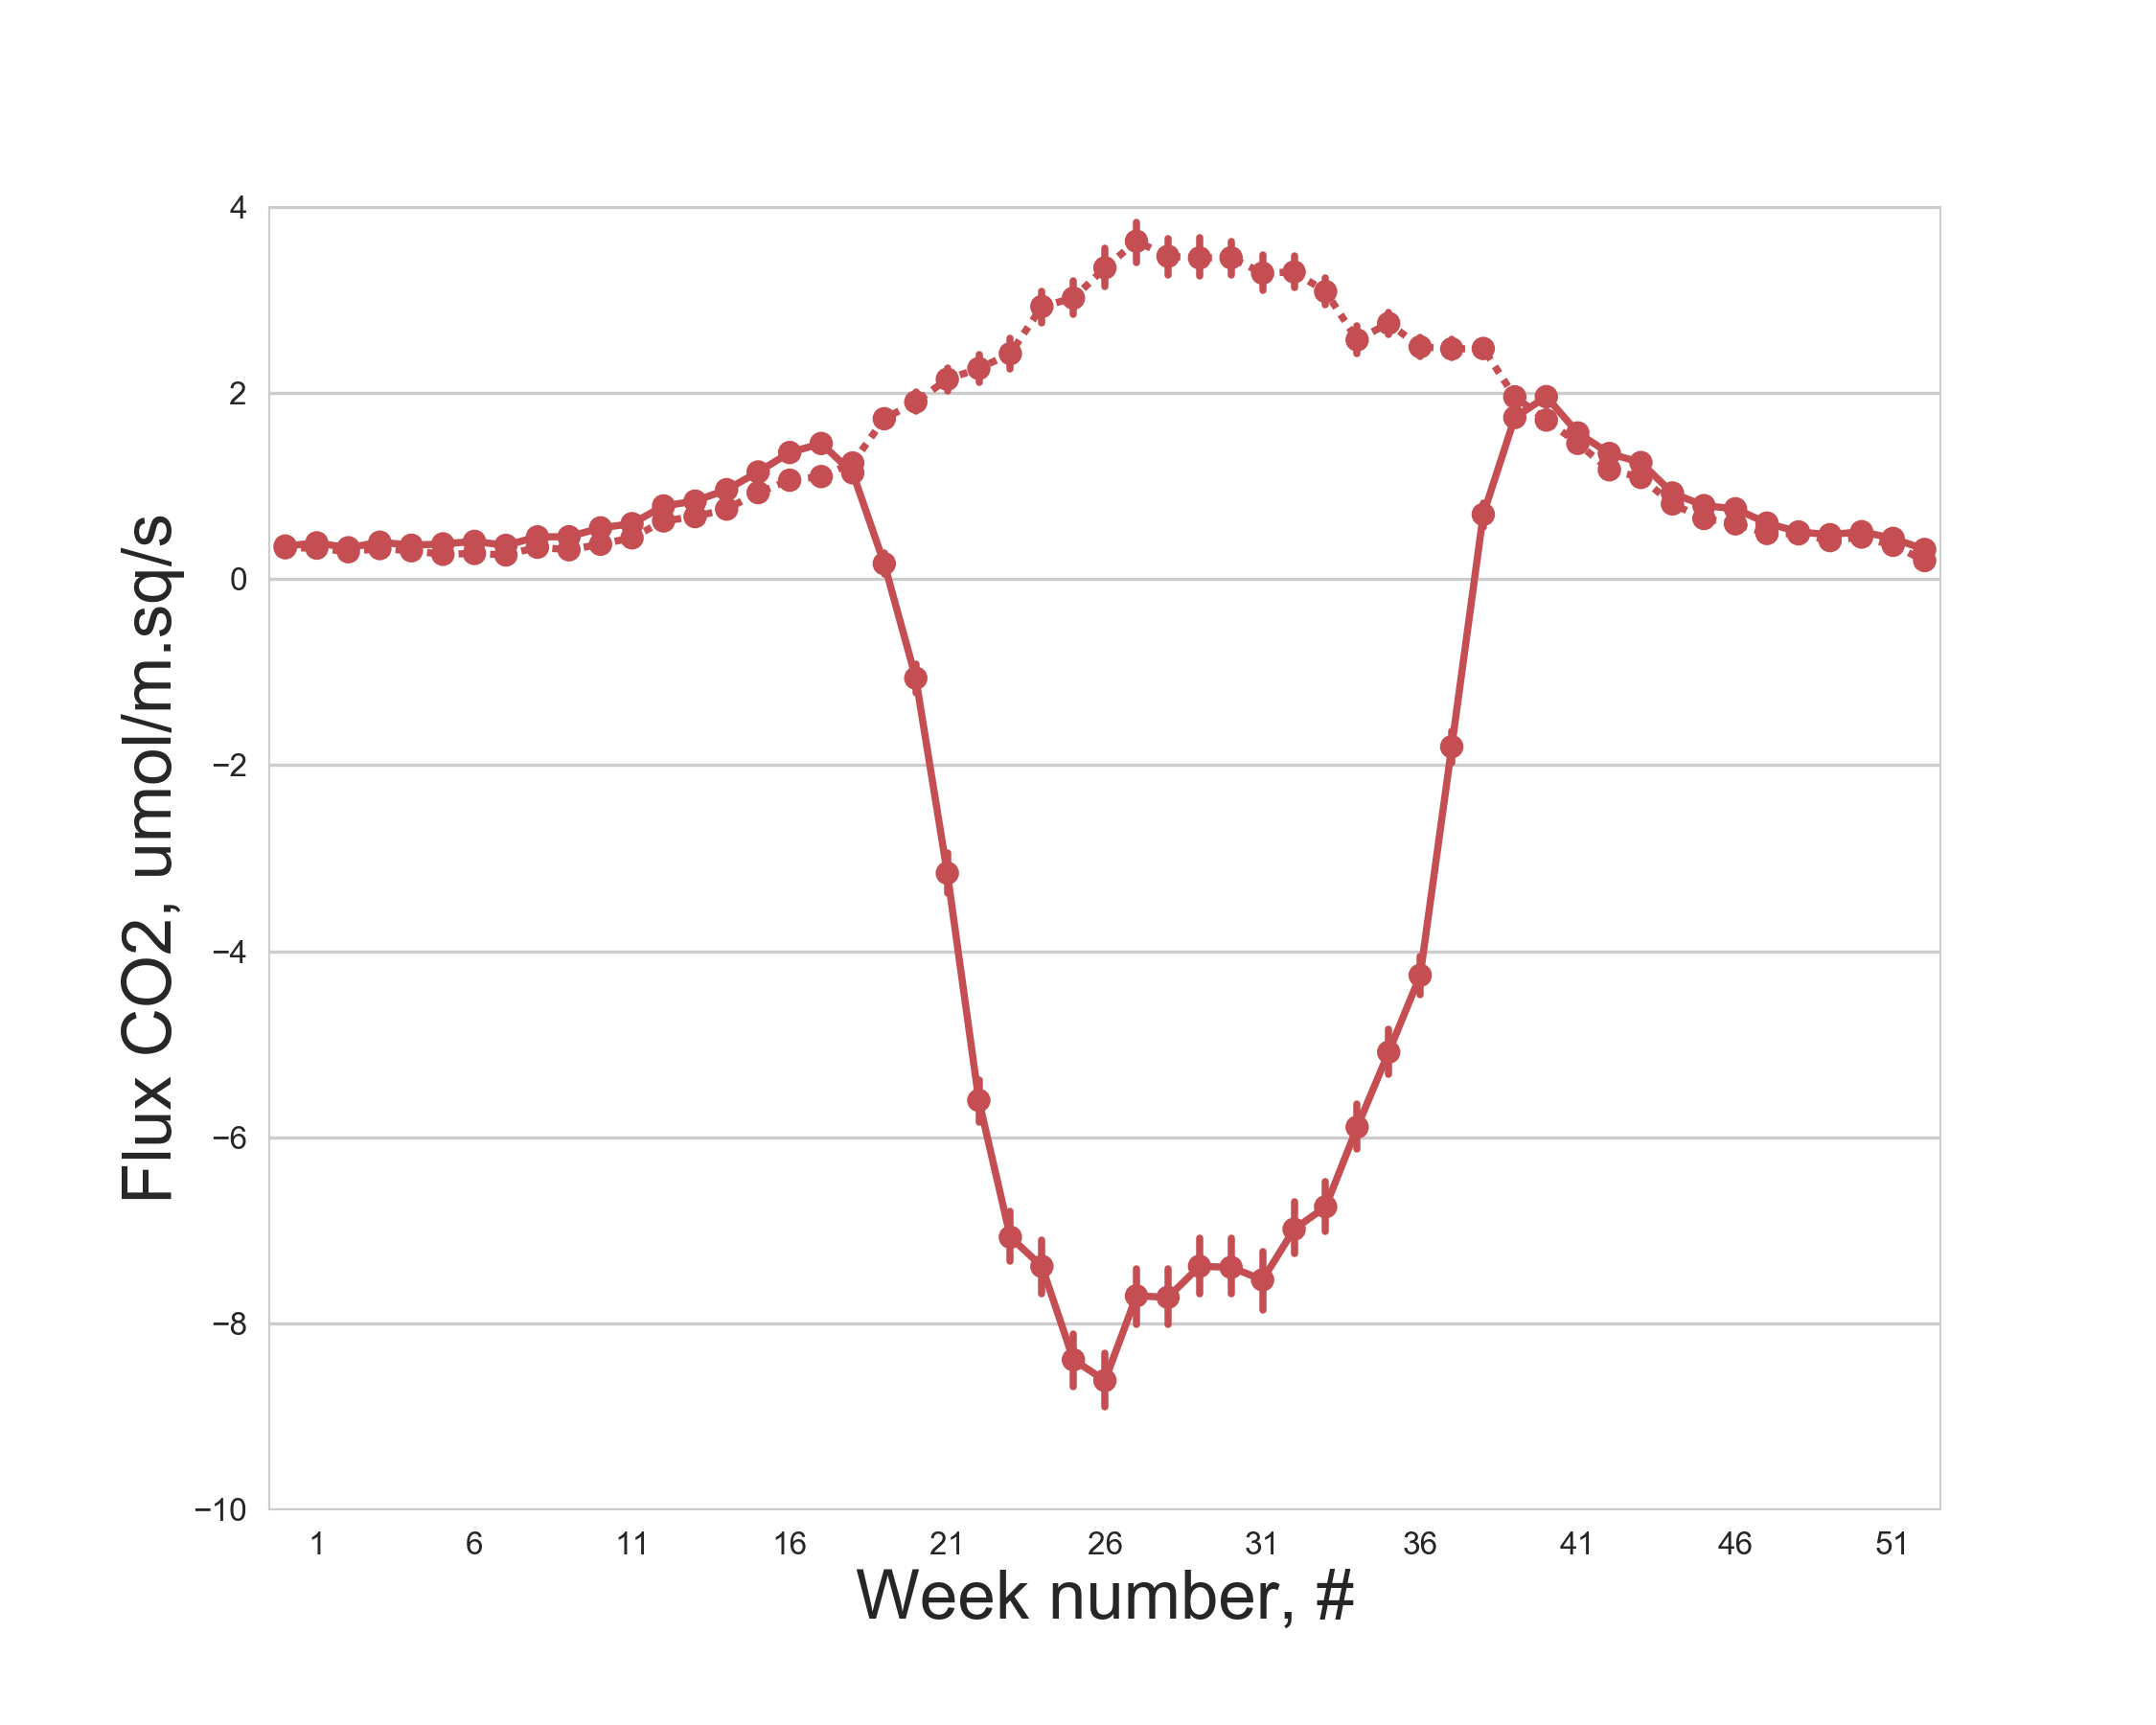
\includegraphics[width=\textwidth]{FvsW_day/CA-Oas.png}
\column{.35\textwidth}
\centering
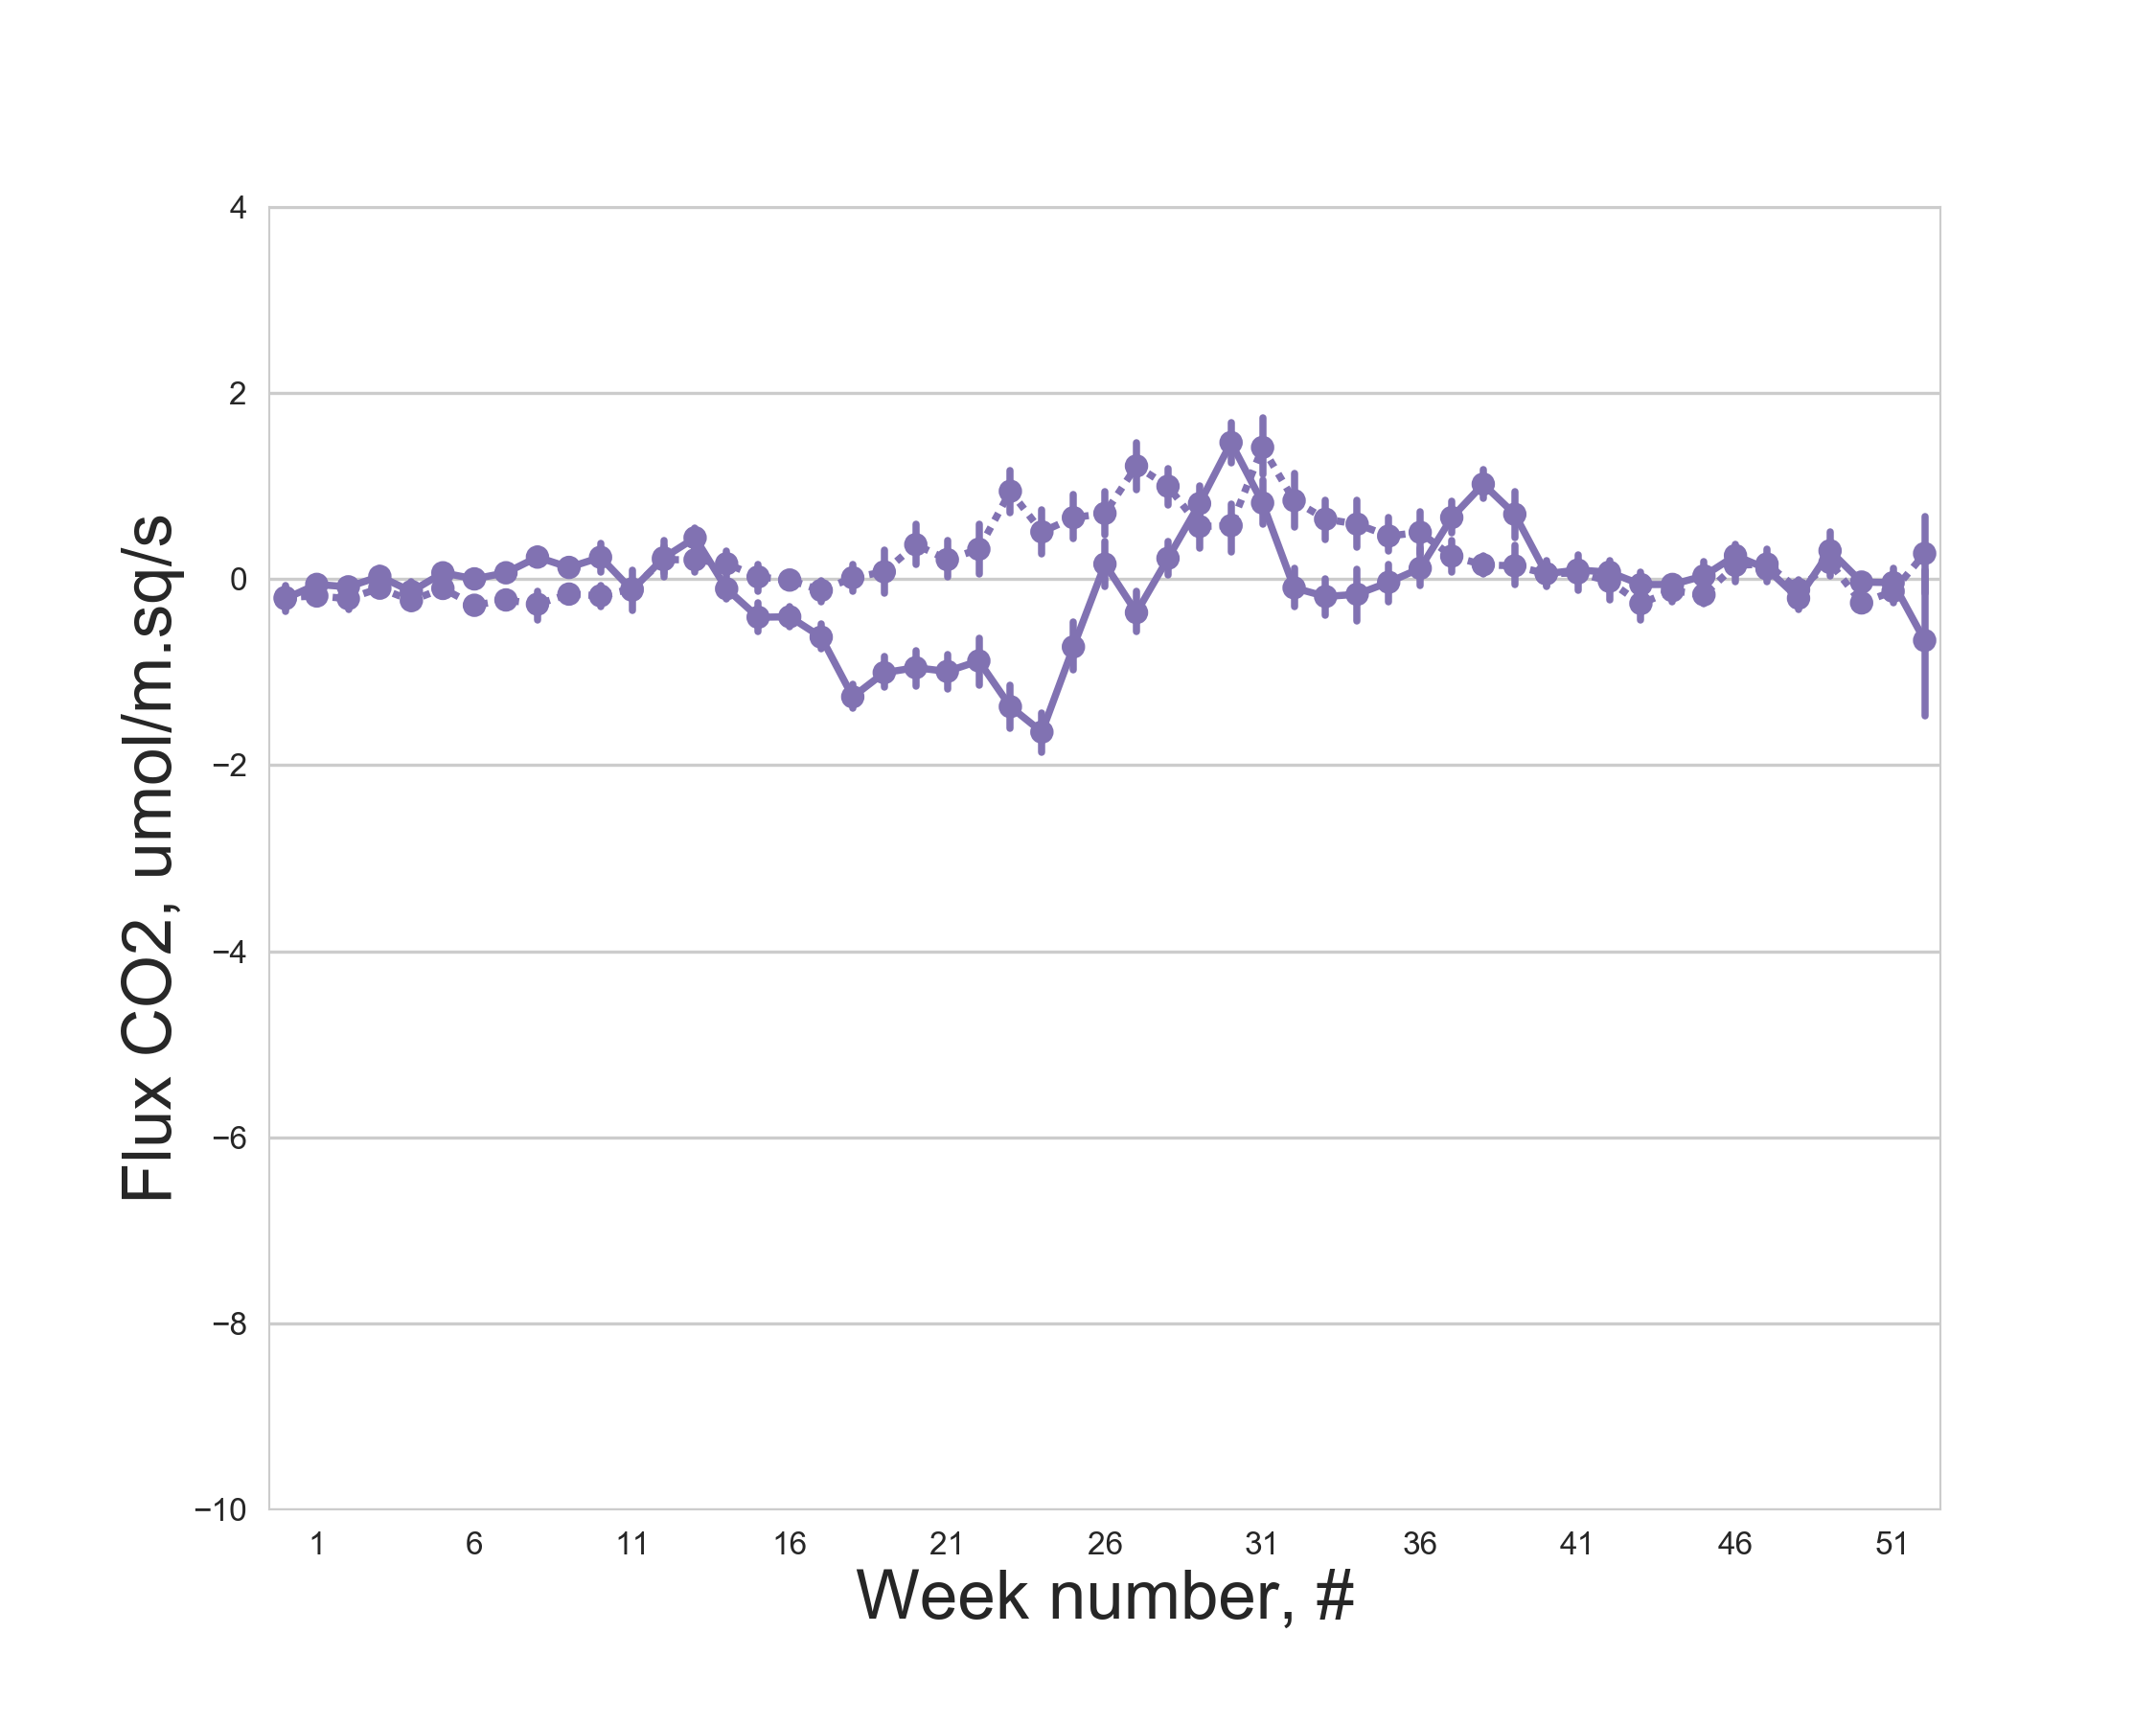
\includegraphics[width=\textwidth]{FvsW_day/US-FPe.png}\\
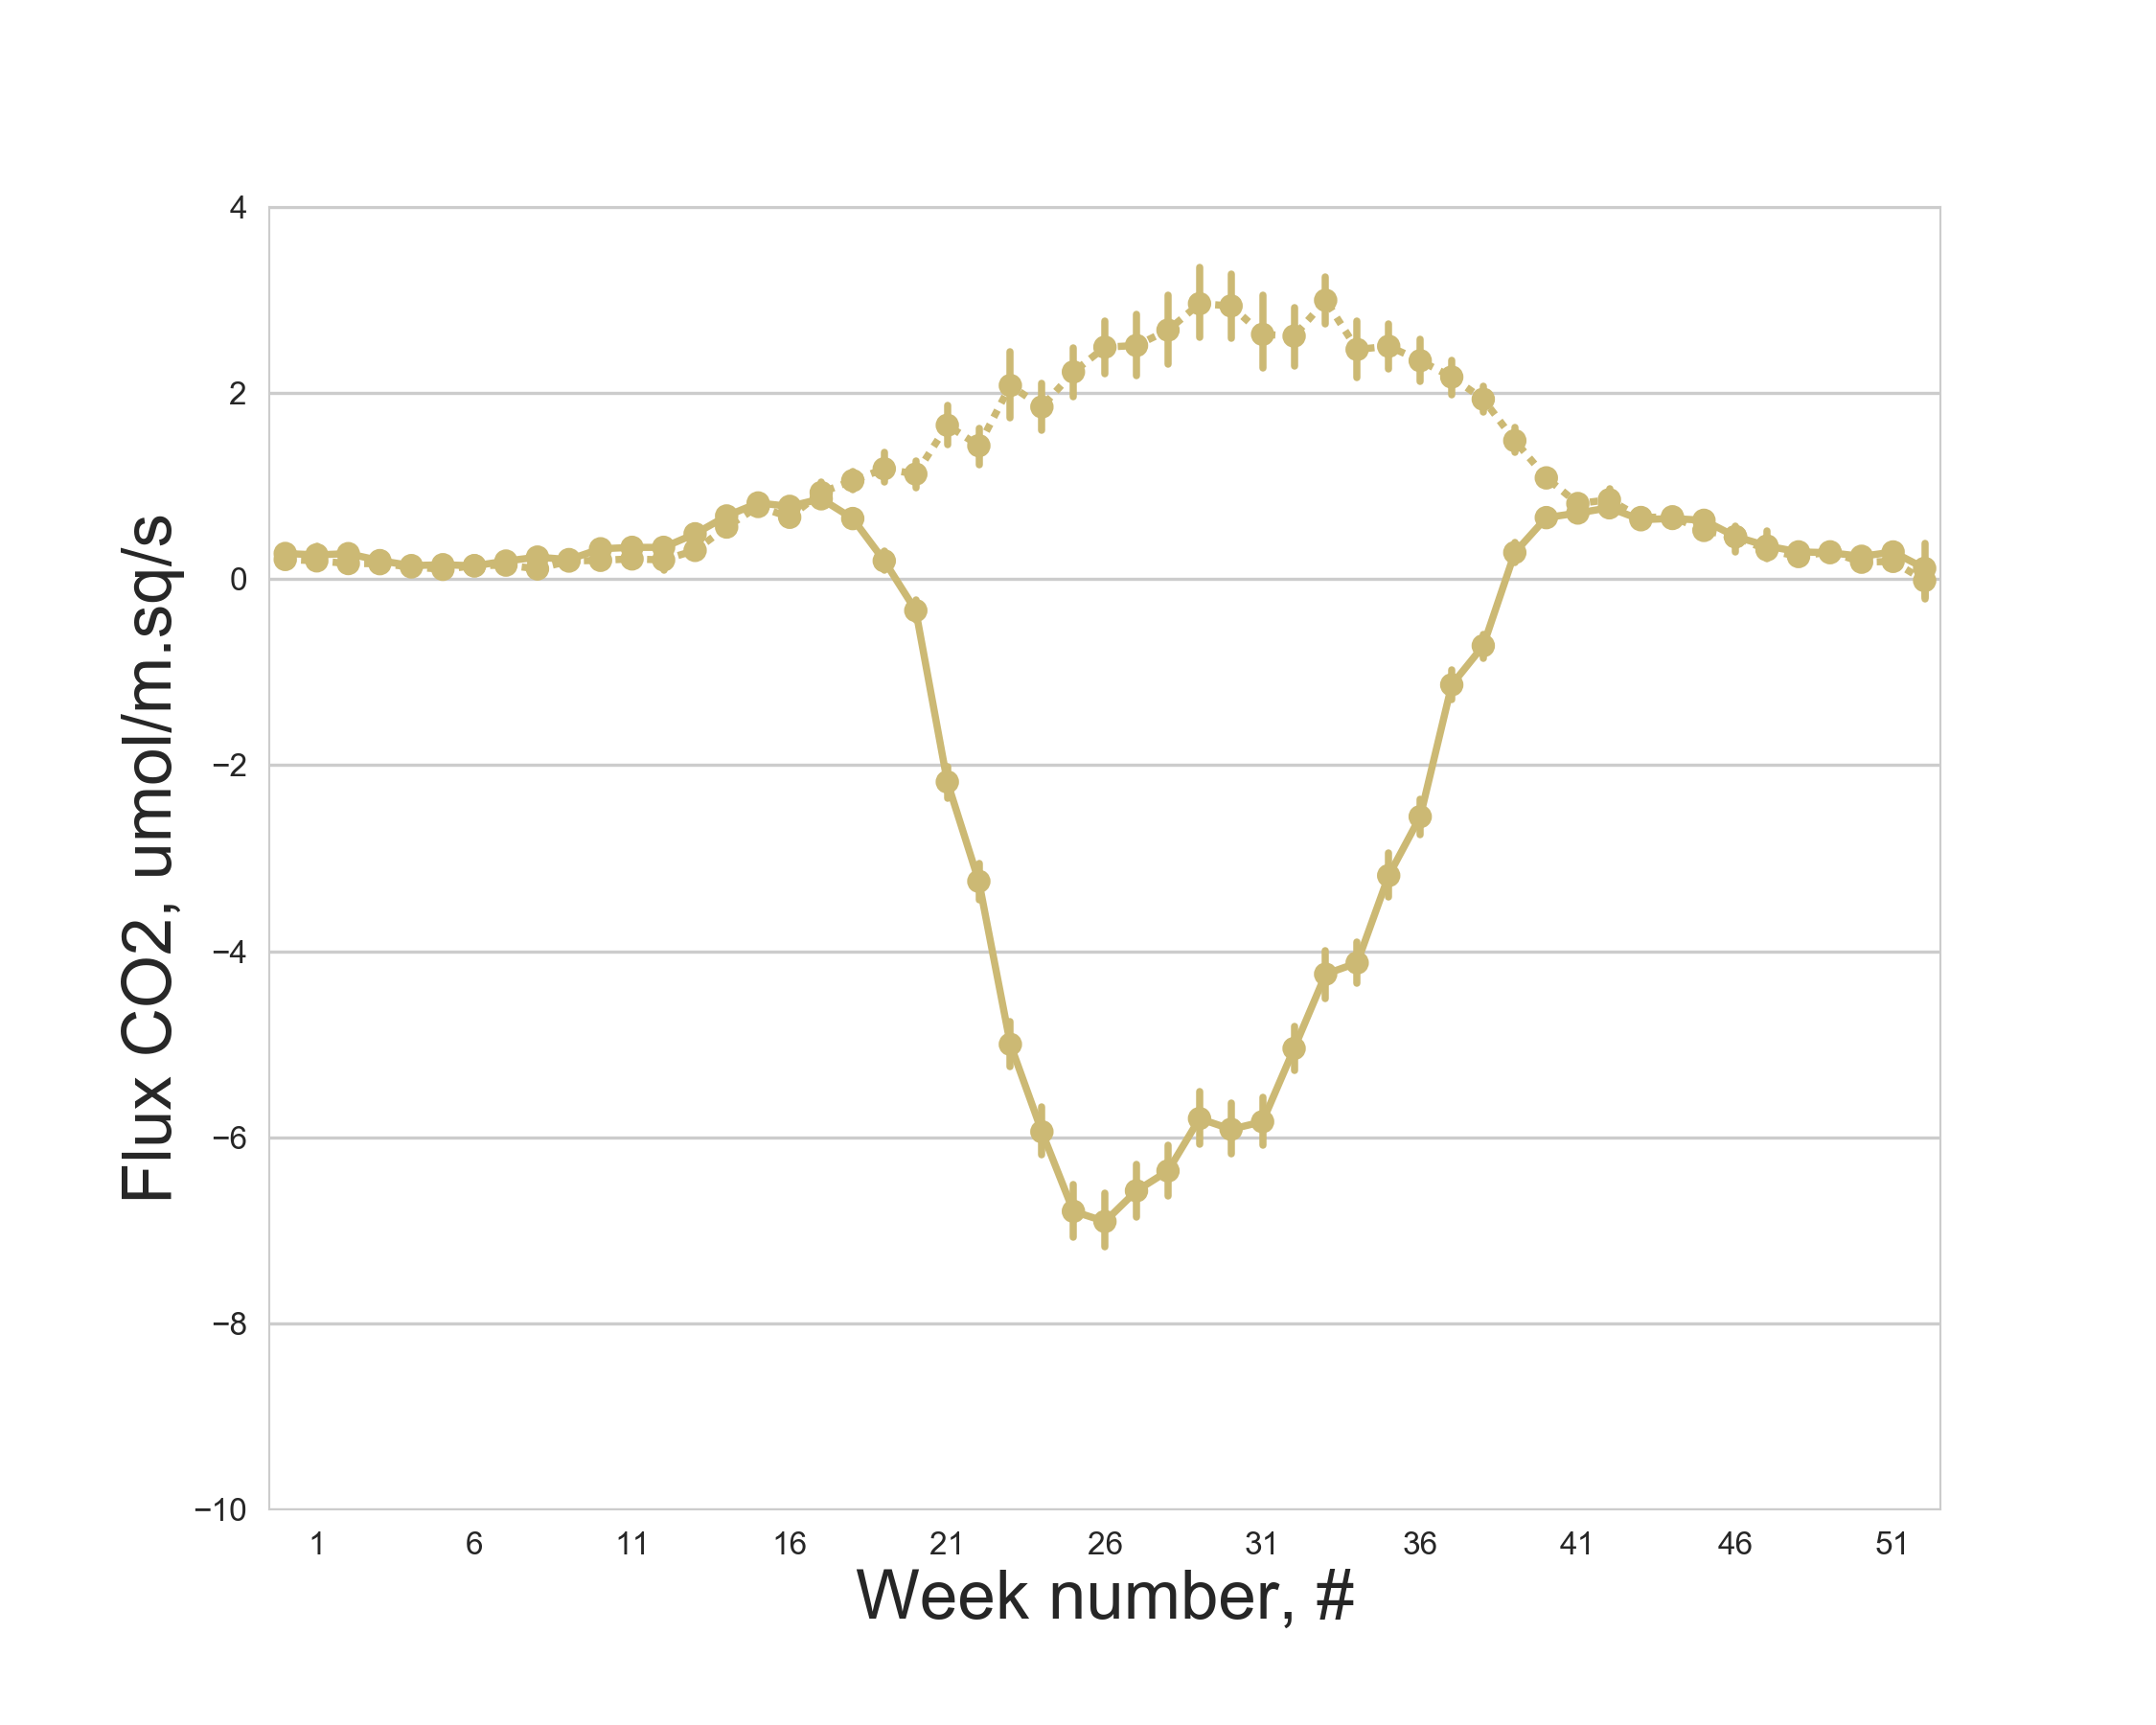
\includegraphics[width=\textwidth]{FvsW_day/US-Los.png}
\end{columns}

\end{frame}


\begin{frame}
\frametitle{Flux vs Temperature at Night}

\begin{columns}[t]
\column{.35\textwidth}
\centering
\includegraphics[width=\textwidth]{FvsT_night/all.png}\\
\includegraphics[width=\textwidth]{FvsT_night/CA-NS1.png}
\column{.35\textwidth}
\centering
\includegraphics[width=\textwidth]{FvsT_night/CA-NS6.png}\\
\includegraphics[width=\textwidth]{FvsT_night/CA-Oas.png}
\column{.35\textwidth}
\centering
\includegraphics[width=\textwidth]{FvsT_night/US-FPe.png}\\
\includegraphics[width=\textwidth]{FvsT_night/US-Los.png}
\end{columns}

\end{frame}

\begin{frame}
\frametitle{Flux vs Temperature during Daylight}

\begin{columns}[t]
\column{.35\textwidth}
\centering
\includegraphics[width=\textwidth]{FvsT_day/all.png}\\
\includegraphics[width=\textwidth]{FvsT_day/CA-NS1.png}
\column{.35\textwidth}
\centering
\includegraphics[width=\textwidth]{FvsT_day/CA-NS6.png}\\
\includegraphics[width=\textwidth]{FvsT_day/CA-Oas.png}
\column{.35\textwidth}
\centering
\includegraphics[width=\textwidth]{FvsT_day/US-FPe.png}\\
\includegraphics[width=\textwidth]{FvsT_day/US-Los.png}
\end{columns}

\end{frame}

\begin{frame}
\frametitle{Flux vs Soil Water Content at Night}

\begin{columns}[t]
\column{.35\textwidth}
\centering
\includegraphics[width=\textwidth]{FvsSWC_night/all.png}\\
\includegraphics[width=\textwidth]{FvsSWC_night/CA-NS1.png}
\column{.35\textwidth}
\centering
\includegraphics[width=\textwidth]{FvsSWC_night/CA-NS6.png}\\
\includegraphics[width=\textwidth]{FvsSWC_night/CA-Oas.png}
\column{.35\textwidth}
\centering
\includegraphics[width=\textwidth]{FvsSWC_night/US-FPe.png}\\
\includegraphics[width=\textwidth]{FvsSWC_night/US-Los.png}
\end{columns}

\end{frame}

\begin{frame}
\setbeamerfont{footnote}{size=\tiny}
\frametitle{Machine Learning Algorithm: Random Forests\footnotemark}
\centering
\includegraphics[width=0.8\textwidth]{random_forest.png}\\
\footnotetext[1]{\textbf{Breiman, L.} \textit{Machine Learning (2001) 45:5.} doi:10.1023/A:1010933404324}
\end{frame}

\begin{frame}
\frametitle{Random Forests Algorithm: Predicted vs Measured (Night)}
\framesubtitle{Features: SWC, T, P, Lat, Long, Date}
\begin{columns}[t]
\column{.4\textwidth}
\centering
% \includegraphics[width=\textwidth]{F_ML/all.png}\\
\includegraphics[width=\textwidth]{F_ML/0.png}\\
\includegraphics[width=\textwidth]{F_ML/1.png}

\column{.4\textwidth}
\centering
\includegraphics[width=\textwidth]{F_ML/2.png}\\
\includegraphics[width=\textwidth]{F_ML/3.png}
\end{columns}
\end{frame}

\begin{frame}
\frametitle{Random Forests Algorithm}
\framesubtitle{Relative Importance of Features}
\centering
\includegraphics[width=0.9\textwidth]{importance.png}\\
\end{frame}


% \begin{frame}
% \frametitle{Random Forests Algorithm: Predicted vs Measured (Night)}
% \framesubtitle{Features: SWC, T}
% \begin{columns}[t]
% \column{.4\textwidth}
% \centering
% % \includegraphics[width=\textwidth]{F_ML/all.png}\\
% \includegraphics[width=\textwidth]{F_ML_2/0.png}\\
% \includegraphics[width=\textwidth]{F_ML_2/1.png}

% \column{.4\textwidth}
% \centering
% \includegraphics[width=\textwidth]{F_ML_2/2.png}\\
% \includegraphics[width=\textwidth]{F_ML_2/3.png}
% \end{columns}
% \end{frame}

% \begin{frame}
% \frametitle{Random Forests Algorithm:}
% \framesubtitle{Relative Importance of Features}
% \centering
% \includegraphics[width=0.9\textwidth]{importance_2.png}\\
% \end{frame}



\begin{frame}
\frametitle{Train on all data (25 Sites). Six Modeled Sites}
\framesubtitle{Modeled Sites:}
\begin{center}
\begin{tabular}{| c | c | c | c | c | c |}
\hline
Station   & Climate & Type & Mean T, C & Mean P, mm & Elev., m\\ \hline
CA-OAS & Dfc     & DBF  & 0.34      & 428        & 530 \\\hline
CA-Qfo & Dfc     & ENF  & -0.36     & 962        & 382 \\\hline
CA-TP3 & Dfb     & ENF  & 8         & 1036       & 184 \\\hline
US-Fpe & Bsk     & GRA  & 5.48      & 335        & 634 \\\hline
CA-TPD & Bsk     & GRA  & 8         & 1036       & 260 \\\hline
CA-GRO & Dfb     & MF   & 1.3         & 831       & 340 \\\hline

\hline
\end{tabular}
\end{center}
\textbf{Climate}:
Dfc - Subarctic: severe winter, no dry season, cool summer;
Bsk - Cold semi-arid climate, steppe, warm winter;
Dfb - Warm Summer Continental: significant precipitation in all seasons.

\textbf{Vegetation}:
ENF - Evergreen Needleleaf Forests;
DBF - Deciduous Broadleaf Forests;
GRA - grassland;
MF - mixed forest;

\end{frame}

\begin{frame}
\frametitle{Random Forests Algorithm: Predicted vs Measured (Night)}
\framesubtitle{Features: SWC, T; Train on all data}

\begin{columns}[t]
\column{.35\textwidth}
\centering
\includegraphics[width=\textwidth]{F_ML_train_all/10.png}\\
\includegraphics[width=\textwidth]{F_ML_train_all/14.png}
\column{.35\textwidth}
\centering
\includegraphics[width=\textwidth]{F_ML_train_all/20.png}\\
\includegraphics[width=\textwidth]{F_ML_train_all/23.png}
\column{.35\textwidth}
\centering
\includegraphics[width=\textwidth]{F_ML_train_all/22.png}\\
\includegraphics[width=\textwidth]{F_ML_train_all/0.png}
\end{columns}

\end{frame}

\begin{frame}
\frametitle{Random Forests Algorithm: Train on all data (25 Sites)}
\framesubtitle{Relative Importance of Features}
\centering
\includegraphics[width=0.9\textwidth]{importance_3.png}\\
\end{frame}



\begin{frame}
\frametitle{Reverse Engineering of Random Forests Algorithm}
\framesubtitle{T dependence}
\centering
\includegraphics[width=0.8\textwidth]{T_dependence.png}\\
\end{frame}


\begin{frame}
\frametitle{Reverse Engineering of Random Forests Algorithm}
\framesubtitle{T dependence}

\begin{columns}[t]
\tiny
\column{.5\textwidth}
\centering
Modified Arrhenius equation for optimum T:
\begin{equation}
    \frac{F}{F_{max}} = \frac{exp\left[\frac{-E_a}{RT_0}\left(1 - \frac{T_0}{T} \right)\right]}{1 + exp\left[ \frac{S T - H_d}{RT} \right]}
\end{equation}

\column{.5\textwidth}
\tiny
\centering
Fitting params:
\begin{align}
T_0 &= 293.4 \text{ K} \\
E_a &= - 22.1 \text{ kJ/mol} \\
S &= 304.1 \text{ J/mol/K} \\
H_d &= 90.6 \text{ kJ/mol}
\end{align}


\end{columns}
% def temp_dep_fun_3(Tk, T0=284.05718055, Ea=-67549.55123981, dS=543.64843782, Hd=155944.4165113):
%     R = 8.314
%     a = np.exp((-Ea/R/T0)*(1-T0/Tk))
%     b = 1+np.exp((Tk*dS-Hd)/Tk/R)
%     return a / b
\centering
\includegraphics[width=0.6\textwidth]{T_dependence_all.png}
\end{frame}



\begin{frame}
\frametitle{Reverse Engineering: Predicted (eq. 6) vs Measured}
\framesubtitle{Measured - solid line; eq. 6 - dashed line}

\begin{equation}
\label{eq:T}
    F = F_{max}\cdot f(T)
\end{equation}

\begin{columns}[t]
\column{.35\textwidth}
\centering
\includegraphics[width=\textwidth]{Reverse_engin_only_T/10.png}\\
\includegraphics[width=\textwidth]{Reverse_engin_only_T/14.png}
\column{.35\textwidth}
\centering
\includegraphics[width=\textwidth]{Reverse_engin_only_T/20.png}\\
\includegraphics[width=\textwidth]{Reverse_engin_only_T/23.png}
\column{.35\textwidth}
\centering
\includegraphics[width=\textwidth]{Reverse_engin_only_T/22.png}\\
\includegraphics[width=\textwidth]{Reverse_engin_only_T/0.png}
\end{columns}

\end{frame}




\begin{frame}
\frametitle{Reverse Engineering of Random Forests Algorithm}
\framesubtitle{$\theta$ dependence}

\centering
\includegraphics[width=0.8\textwidth]{Theta_dependence_30.png}

\end{frame}


\begin{frame}
\frametitle{Reverse Engineering of Random Forests Algorithm}
\framesubtitle{$\theta$ dependence}

\centering
\includegraphics[width=0.8\textwidth]{Theta_dependence_20.png}

\end{frame}

\begin{frame}
\frametitle{Reverse Engineering of Random Forests Algorithm}
\framesubtitle{$\theta$ dependence}

\centering
\includegraphics[width=0.8\textwidth]{Theta_dependence_10.png}

\end{frame}

\begin{frame}
\frametitle{Reverse Engineering of Random Forests Algorithm}
\framesubtitle{$\theta$ dependence}

\centering
\includegraphics[width=0.8\textwidth]{Theta_dependence_0.png}

\end{frame}


\begin{frame}
\frametitle{Reverse Engineering of Random Forests Algorithm}
\framesubtitle{$\theta$ dependence}

\begin{columns}[t]
\tiny
\column{.5\textwidth}
\begin{equation}
    \frac{F}{F_{max}} = \sum\limits^{4}_i A_i\frac{1}{\sqrt{2\pi \sigma_i^2}} e^{- \frac{(x - \mu_i)^2}{2\sigma_i^2}}
\end{equation}
\column{.5\textwidth}
\tiny
\centering
Fitting params: \\
\begin{tabular}{|c|c|c|c|c|}
 \hline
 Parameter & a    & b    & c    & d\\ \hline
 A         & 0.85  & 0.5 & 0.5  & 0.3 \\ \hline
 $\mu$     & 0.11 & 0.37 & 0.71 & 1.1 \\ \hline
 $\sigma$  & 0.04 & 0.1 & 0.1  & 0.2 \\ \hline

\end{tabular}

\end{columns}
% mu1=0.11, sig1=0.04, mu2=0.37, sig2=0.07, mu3=0.71, sig3=0.1, mu4=1.1, sig4=0.2


\centering
\includegraphics[width=0.7\textwidth]{Theta_dependence_fit.png}

\end{frame}


\begin{frame}
\frametitle{Reverse Engineering: Predicted (eq. 8) vs Measured}
\framesubtitle{Measured - solid line; eq. 8 - dashed line}

\begin{equation}
\label{eq:TO}
    F = 0.75F_{max}\cdot f(T) + 0.25F_{max}\cdot f(\theta)
\end{equation}

\begin{columns}[t]
\column{.35\textwidth}
\centering
\includegraphics[width=\textwidth]{Reverse_engin/10.png}\\
\includegraphics[width=\textwidth]{Reverse_engin/14.png}
\column{.35\textwidth}
\centering
\includegraphics[width=\textwidth]{Reverse_engin/20.png}\\
\includegraphics[width=\textwidth]{Reverse_engin/23.png}
\column{.35\textwidth}
\centering
\includegraphics[width=\textwidth]{Reverse_engin/22.png}\\
\includegraphics[width=\textwidth]{Reverse_engin/0.png}
\end{columns}

\end{frame}




\end{document}
